\documentclass{kththesis}

\justifying
\usepackage{graphicx}
\usepackage{epigraph}
\usepackage{bm}
\usepackage{hyperref}
\usepackage{cleveref}
\usepackage{todo}
\usepackage{subcaption}
\usepackage{float}
\usepackage[chapter]{algorithm}
\usepackage{algorithmic}
\usepackage{amsmath}
\usepackage{multirow}
\usepackage{booktabs}
\usepackage{adjustbox}
\usepackage{listings}

\newtheorem{definition}{Definition}

% remove this if you are using XeLaTeX or LuaLaTeX
\usepackage[utf8]{inputenc}

% Use natbib abbreviated bibliography style
\usepackage[square,numbers]{natbib}
\bibliographystyle{unsrtnat}

\usepackage{lipsum} % This is just to get some nonsense text in this template, can be safely removed

\title{Predicting user churn on streaming services using recurrent neural networks}
\alttitle{Förutsägande av användarens avbrott på strömmande tjänster med återkommande neurala nätverk}
\author{Helder Martins}
\email{helder@kth.se}
\supervisor{Hedvig Kjellström (KTH) and Sahar Asadi (Spotify)}
\examiner{Patric Jensfelt}
\programme{Master in Machine Learning}
\school{School of Computer Science and Communication}
\date{\today}


\begin{document}

% Title page
\flyleaf

\begin{abstract}
Providers of online services have witnessed a rapid growth of their user base in the last few years. The phenomenon has attracted an increasing number of competitors determined on obtaining their own share of the market. In this context, the cost of attracting new customers has increased significantly, raising the importance of retaining existing clients. Therefore, it has become progressively more important for the companies to improve user experience and ensure they keep a larger share of their users active in consuming their product. Companies are thus compelled to build tools that can identify what prompts customers to stay and also identify the users intent on abandoning the service. The focus of this thesis is to address the problem of predicting user abandonment, also known as \emph{churn}, and also detecting motives for user retention on data provided by an online streaming service. 

Classical models like logistic regression and random forests have been used to predict the churn probability of a customer with a fair amount of precision in the past, commonly by aggregating all known information about a user over a time period into a unique data point. On the other hand, recurrent neural networks, especially the long short-term memory (LSTM) variant, have shown impressive results for other domains like speech recognition and video classification, where the data is treated as a sequence instead. This thesis investigates how LSTM models perform for the task of predicting churn compared to standard nonsequential baseline methods when applied to user behavior data of a music streaming service. It was also explored how different aspects of the data, like the distribution between the churning and retaining classes, the size of user event history and feature representation influences the performance of predictive models. The obtained results show that LSTMs has a comparable performance to random forest for churn detection, while being significantly better than logistic regression.  Additionally, a framework for creating a dataset suitable for training predictive models is provided, which can be further explored as to analyze user behavior and to create retention actions that minimize customer abandonment.
\end{abstract}

\clearpage

\begin{otherlanguage}{swedish}
  \begin{abstract}
Leverantörer av onlinetjänster har bevittnat en snabb användartillväxtunder de senaste åren. Denna trend har lockat ett ökande antal konkurrenter som vill ta del av denna växande marknad. Detta har resulterat i att kostnaden för att locka nya kunder ökat avsevärt, vilket även ökat vikten av att behålla befintliga kunder. Det har därför gradvis blivit viktigare för företag att förbättra användarupplevelsen och se till att de behåller en större andel avanvändarna aktiva. Företag har därför ett starkt intresse avatt bygga verktyg som kan identifiera vad som driver kunder att stanna eller vad som får dem lämna. Detta arbete fokuserar därför på hur man kan prediktera att en användare är på väg att överge en tjänst, så kallad “churn”, samt identifiera vad som driver detta baserat på data från en onlinetjänst.
   
Klassiska modeller som logistisk regression och random forests har tidigare använts på aggregerad användarinformation över en given tidsperiod för att med relativt god precision prediktera sannolikheten för att en användare kommer överge produkten.  Under de senaste åren har dock sekventiella neurala nätverk (särskilt LSTM-varianten Long Short Term Memory), där data istället behandlas som sekvenser, visat imponerande resultat för andra domäner såsom taligenkänning och videoklassificering. Detta arbete undersöker hur väl LSTM-modeller kan användas för att prediktera churn jämfört med traditionella icke-sekventiella metoder när de tillämpas på data över användarbeteende från  enmusikstreamingtjänst. Arbetet undersöker även  hur olika aspekter av data påverkar prestandan av modellerna inklusive distributionen mellan gruppen av användare som överger produkten mot de som stannar, längden av användarhändelseshistorik och olika val av användarfunktioner för modeller och användardatan. De erhållna resultaten visar att LSTM har en jämförbar prestanda med random forest för prediktering av användar churn  samt är signifikant bättre än logistisk regression. LSTMs visar sig således vara ett lämpligt val för att förutsäga churn på användarnivå. Utöver dessa resultat utvecklades även ett ramverk  för att skapa dataset som är lämpliga för träning av prediktiva modeller, vilket kanutforskas ytterligare för att analysera användarbeteende och för att skapa förbättrade åtgärder för att behålla användare och minimera antalet kunder som överger tjänsten.
  \end{abstract}
\end{otherlanguage}

\clearpage

\cleardoublepage

\tableofcontents

\listoffigures
 
\listoftables


% This is where the actual contents of the thesis starts
\mainmatter


\chapter{Introduction}

		In a world where service providers face an ever-increasing competition on the market, retaining the already acquired customers is rising in importance for any company that wants to stay in business. This is specially true for industries that are mainly web-based: startups nowadays can provide an online service with  an impressively low amount of initial capital, entering into a new market with relative ease. While ousting a well-established company from the top is a hard feat to accomplish, it is far from being an unheard event, urging business to set up specialized tools to identify unsatisfied clients and plan retention actions. 
		
	The act of a user abandoning a service provider, either by discontinuation of a formal contract or inactivity, is called \emph{churn}. Customer relationship management tools aim to minimize the share of churned uses to increase profitability and improve business health. For doing so, an important step that must be performed is to identify the users more likely to churn in the near future. The task of detecting how likely a user is to abandon a service is called \emph{churn prediction}, and it is the main subject of this thesis.
	
	Predicting whether a user is going to leave the service provider in the near future is a subject that has received some attention in academia in the past few years \citep{Pudipeddi2014}\citep{GurAli2014}\citep{Drachen2016RapidPO}. Models like logistic regression and random forests are popular choices for this task \citep{mahajan2015review}, however most of the work in the area has a common trait regarding the way the data is represented before being used for model training: features are aggregated over a time span into a single data point for each user, normally through a mean function. Even though this approach simplifies the task of training the predictive models, latent temporal factors hidden in the sequence that could prove useful for increasing the performance of estimators are inherently lost in this process. For instance, a customer who is gradually reducing their usage of the service over time can be thought as having a higher chance of churning in the future, a property that would be lost if the feature is aggregated over the whole time span. Meanwhile, the long short-term memory (LSTM) recurrent neural network has recently shown positive results for domains like speech recognition \citep{graves2013speech} and video classification \citep{yue2015beyond} where the data is naturally represented as a sequence. This thesis work studies how the temporal factors hidden in the user behavior data, allied with a model that can leverage it, compares to the state of the art for predicting user abandonment. Three models were thus chosen for this task: logistic regression and random forests representing the nonsequential aggregated models, and LSTM as the sequential estimator.	
	
	With the advent of big data technologies and cloud providers, the burden of storing large quantities of user data has been mostly lifted, allowing companies to store information about customers behavior on the application with moderate engineering effort. The overwhelming amount of information available however poses its own set of challenges when it comes to using this data for a specific task; choosing the best user attributes for a certain problem is far from trivial: choose too few and the task may be unsolvable, choose too many and the important information might be lost in a sea of irrelevant data. Similarly, the available features may fail to represent the user attitude towards the service in its raw state, requiring  new features to be engineered to capture this information. Therefore, creating a dataset that is suitable for detecting the user disposition towards churning and retaining will be an important topic in this thesis work as well.
	
	This thesis has been defined as a master thesis work at \emph{Spotify}. I have been given access to computational resources and pseudonymized user data to investigate user churn.
      
\section{Research Question}	
	
The main research question of this project is:

\begin{itemize}
\item Which predictive modeling algorithm between logistic regression, random forests and LSTM obtains the best performance for predicting the probability of a user towards churning the service provider in the future?
\end{itemize}	

An auxiliary research question is:

\begin{itemize}
\item How do different aspects of the data, like the class distribution between churning and retaining users, the amount of historical user behavior information used for training, and different representations for the data influence the accuracy of the predictive models?
\end{itemize}

\section{Limitations}

The data available will be limited to user activity information observed during the period of 90 days. Also, due to the large volume of user information available, a sampling technique was used to limit the size of the data as to fit into the scope of the project.

\section{Sustainability, Ethical and Social Aspects}

The protection of user personal data has reached the spotlight in recent years, mainly through its misuse by companies that detain this kind of information. With the widespread use of mobile devices connected to the Internet 24/7, several service providers have at their disposal an immense quantity of customer data as fine-grained as user's location, purchase behavior in e-stores and more. Users are commonly unaware of how their data is being exploited by providers, the exact definition being hidden in thousands of lines in a software agreement written in an obscure way that even specialists may fail to comprehend. Even if fully understood, the legality of its terms is being questioned by courts of law around the world. To protects its citizen's digital data, the European Union has recently issued a set of laws concerning data privacy that shall be put into practice in May 2018 \citep{eu2017protection}.

The misuse of customer information by companies that sparked these concerns has its fair share of examples in the wild. For instance, the company Facebook released a controversial study where it manipulated the sentiments of its users by feeding into its client's news feed articles leaning towards a positive and negative sentiment, and analyzing how users responded to that stimulus\citep{kramer2014experimental}. However no user was aware of this manipulation, which could inadvertently lead to tragic outcomes that the experimenters failed to consider. 

Another notorious example came from a contest sponsored by Netflix for researchers who could improve its recommendation algorithm, an event known as "the Netflix Prize" \citep{bennett2007netflix}. The massive dataset containing user behavior information on its video platform, alongside a prize of 1 million dollars for the winning team, gathered the interest of researchers all around the world. However a major class-action suit was filled against the company for failing to anonymize user information properly with customers claiming that they could be uniquely identified through the released data, and the outcome was Netflix canceling future versions of the contest altogether \citep{wired2010netflix}.

The protection of user privacy is a key component in Spotify's business model. Being a company primarily data-driven, it is imperative that Spotify can be trusted in the public's eyes as a custodian of customers' data, both for increasing the user satisfaction with the service and also to avoid similar legal processes suffered by other companies that might deter it from its main mission and priorities. With that in mind, Spotify take steps as to make sure that privacy, security and encryption of its user data complies with the applicable law. This thesis work is based on pseudonymized user data to investigate user churn. 

The computing resources utilized in this project were provided mainly by Google's Cloud Platform data centers. These clusters of machines were heavily optimized throughout the years as to efficiently make use of energy resources, in a way that most companies are incapable of due to technology and budget constraints. A recent announcement revealed that in 2017 every data centers owned by Google will run on 100\% renewable energy, which is a feat that few other companies can claim \citep{google2017renew}.  

\section{Contributions}

The main contributions of this project can be listed as:

\begin{itemize}
\item Evaluating the performance of a recurrent neural network model compared to the commonly used techniques used for churn prediction.
\item Assessing the impact that the size of the customer event history has on the accuracy of the trained predictive models.
\item Analyzing the performance of models when predicting churn for increasing time ranges in the future.
\item Experimenting on changing the ratio between the retained and churning classes, and the impact in accuracy that it yields.
\item Evaluating the impact a lower dimensional representation of user data has on the performance of predictive models.
\item A data pipeline suitable for extracting sequential information from raw user data as to build predictive models tailored to the service provider.
\end{itemize}

\section{Outline}

This thesis is organized as follows. \Cref{cha:background} introduces key concepts that will be important for the proper understanding of this report. It is followed by \Cref{cha:related_work}, where the current state-of-the-art in churn prediction techniques will be presented to the reader, while also exposing the literature on time-series modeling and how it can be applied for the task at hand. 

In \Cref{cha:data} a detailed description on how the dataset used for training the classifiers was created will be given, followed by a brief exploration of the generated data. In \Cref{cha:method}, the reader will be presented to the methods utilized for performing the experiments in this project. It will delve into how the training of the models was performed, how the parameters were optimized, and how the final score for each classifier was obtained.

\Cref{cha:results} will be dedicated to present to the reader the main results obtained from the experiments performed in the project, which will be discussed on \Cref{cha:discussion}. \Cref{cha:conclusion} summarizes the work performed in this project. Additional extensive results are presented in \Cref{cha:add_results}. 

\chapter{Background}
\label{cha:background}

For a better understanding of this degree project, some concepts are required to be properly introduced. Some of them are mainly application-specific, while others pertain to how we decided to represent the data, which algorithms we decided to use in our experiments and how the data was manipulated and transformed. 

	\section{Streaming Services}
	
	The rise of streaming services has in recent years revolutionized the way customers get access to digital content. The traditional model of media ownership, even though it still represents a significant share of revenue, is continuously losing ground to a new right-of-access model where users get access to content ether by paying a monthly subscription or with limited free access while also being exposed to advertisement. The customer base of said services is steadily growing, and with it the amount data collected tracking how they interact with the provided digital media. This information is of high-value to any provider who expects improve the user experience, increase its total number of clients and also avoid losing the current ones to the competition.

	Applications like Netflix and Spotify have changed the industry by offering a legal and affordable way of accessing content through a subscription-like contract instead of the classical pay-by-content commonly used by traditional media providers. This change in business model has proven to be successful by the sheer amount of customers that the most popular service providers have today. Netflix for instance has reported to its shareholders a user base of 93 million worldwide at the end of 2016 \citep{netflixsh}, while Spotify recently reached the amazing feat of 50 millions paying subscribers, 20 millions of that only in one year \citep{spotifypress}. The adoption of this new model by consumers indicates no interest of going back to the old ways of getting access to digital content, for example through physical or downloadable pay-by-content media.

	\begin{figure}[h]
    \centering
    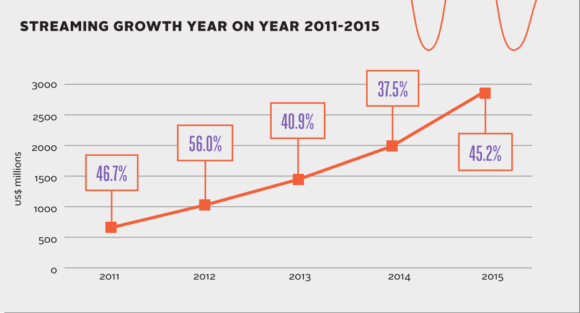
\includegraphics[width=0.7\textwidth, natwidth=580bp, natheight=313bp]{figures/ifpi_stream_growth.png}
    \caption{IFPI's streaming growth report}
    \label{fig:ifpi-growth-report}
\end{figure}

	Music streaming follows this trend of growth on the latest economical reports. Over a five-year period ending in 2015, the observed revenue from the industry grew four times to US \$2.89 billion as can be seen in \Cref{fig:ifpi-growth-report} from the International Federation of the Phonographic Industry (IFPI) organization \citep{ifpi}. The increase in the number of paying subscribers is also notable, seeing an increase from 8 to 68 millions people over the same period. This new model also helped bring some countries like China and Mexico where licensed music market was losing grounds to piracy, and it corresponds to around 20\% of the industry's revenue in the top five markets in the world \citep{ifpi}. 
	  
\section{Customer Churn and Retention} 

\emph{Customer churn}, also known as turnover or defection, is defined as the amount of customers who cut ties with the service provider or company. The rate at which the user base defects from the service provider is widely considered a good indicator of business health. The ability of a company retaining its clients over a specific period of time, is called \emph{customer retention}. Firms that have a high share of users that return to the provided service possess high retention, a property that posses a non-linear relationship with customer satisfaction metrics \citep{hennig1997impact}. Low retention on the other hand indicates the inability of a company keeping its user base for a long period of time, which can be interpreted as users being displeased with the products they have been offered. A study performed on a bank firm in Brazil also showed how retention metrics are positively correlated to profitability measures of a business \citep{morgan2006value}. 
        
Every company that wants to keep being relevant in a competitive market should strive to retain its user base and minimize user defection. Understanding the reasons that justify user behavior on the platform is critical for the planning of successful retention actions. With that goal, an important step is to identify which features of the data have a strong correlation with the probability of a user churning or not. With that information, the providers could for example set up automated actions as to influence the value on these features. Learning which are the most important features is also of relevance for the task of choosing what data to use for training the predictive models, since training models with a full dataset will commonly introduce error on the system and take a large amount of computing resources to train.

Every service provider has a different definition of what churn is. Some of them use the explicit cancellation of a contract as indicator of user abandonment, which has the advantage of being straightforward to calculate and having a clear correlation to revenue metrics, while others prefer to explore the user activity instead, which has the benefit of better leveraging his satisfaction level and working with the assumption that a satisfied customer has a lower chance of leaving the service for the competition. In this degree project, the \emph{user activity} will be used to define churn. Thus engagement through media consumption will be used as a measure for labeling users as churning or retained, disregarding whether users are paying customers or not.

\section{Time Series and Aggregated Data}
\label{sec:timewindows}

In this section we introduce some concepts that explores the sequential nature of user data. Consider $\mathbf{x}_{nt}$ as the $D$-dimensional vector representing the features of user $n=1,...,N$ at time step $t = t_0,...,t_{\alpha+\beta}$, with $t$ being an equally spaced and discrete time. Now consider that the intervals are split into two sequential and non-overlapping time windows: an \emph{observation window} where $t = t_0,...,t_\alpha$ which is going to be used for observing user behavior, and a \emph{prediction window} where $t = t_{\alpha+1},...,t_{\alpha+\beta}$ used for evaluating if a user churned or not, with $\alpha$ and $\beta$ being the size of each of the respective windows. A third \emph{activity window} where $t=t_{\alpha-\gamma},...,t_\alpha$ overlaps with the last $\gamma$ time steps of the observation window and it is used for sampling active users, which is important to avoid sampling users that churned a long time ago. The time windows can be better seen in \Cref{fig:timewindows}.

\begin{figure}[h]
    \centering
    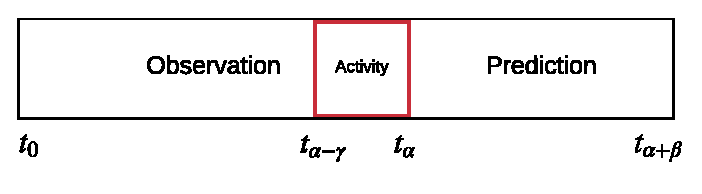
\includegraphics[width=0.7\textwidth,keepaspectratio]{figures/timewindows.pdf}
    \caption{The time windows}
    \label{fig:timewindows}
\end{figure}

\begin{definition}
The action of delivering media content to an end-user from a service provider is called a \emph{stream}. A stream is initiated when the user starts consuming the media content through any of the provider's supported platforms, and the stream ends when this action stop either voluntarily by the user or for a number of technical reasons.
\end{definition}

\begin{definition}
A user is considered to be \emph{active} during a time period if he has one or more streams of any length, and \emph{inactive} otherwise.
\end{definition}

Being $\mathbf{x}_n$ a sampled user who is active in the activity window, $y_{n}$ is the variable specifying if customer $n$ has churned between time steps $t_{\alpha+1}$ and $t_{\alpha+\beta}$ of the prediction window, such as

\begin{equation}
y_n = \\ 
\begin{cases}
  \text{0 if user $n$ is active between $t_{\alpha+1}$ and $t_{\alpha+\beta}$} \\    
  \text{1 otherwise}    
\end{cases}
\end{equation}

which assigns one label per customer in our dataset. A user is said to have \emph{churned} if the label is positive, and \emph{retained} otherwise (sometimes called the negative class). This definition follows business metrics originated from the service provider, where the counting of active users over a predetermined time span is one of the key metrics indicating business health. For instance, a $\beta$ corresponding to 30 days would yield whether the customer will be a monthly active user the following month after being observed for $\alpha$ time steps. 

The literature on churn prediction commonly describes the user features as a single point over the whole observation period, ignoring the time component of the data by transforming it through an aggregation function like the mean. As to train our non-sequential predictive models, we need a similar representation of the data which summarizes information available about a user behavior over time into a single $D$-dimensional vector. Following the work by \citep{GurAli2014}, we define a \emph{single period training data (SPTD)} as the dataset consisting of one observation per customer who is active during the sampling period. In this approach, the dataset is 

\begin{equation}
\text{SPTD} = [\mathbf{X}_{t_0 \rightarrow t_\alpha}, \mathbf{y}]
\end{equation}

where $\mathbf{X}_{t_0\rightarrow t_\alpha}$ is a $N \times D$ matrix consisting of the constructed features $f(\mathbf{X})$, $f$ is a feature aggregation function that maps all $\alpha$ user vectors over the observation window to a single one with the same number of $D$ features, and  $\mathbf{X}$ as the $N \times \alpha \times D$ matrix containing information about all users over the whole observation period. $\mathbf{y}$ is a $1 \times N$ column vector containing churn labels for all samples. 

While the simple format of SPTD can be used for training most types of predictive models, it is unsuitable when the goal is to leverage the sequential properties of the data since it is destroyed after the aggregation function. Thus, we define a \emph{multiple period training data (MPTD)} as

\begin{equation}
\text{MPTD} = \\
\left [  
  \begin{tabular}{c c}
   $\mathbf{X}_{t_0}$   & \multirow{4}{*}{y} \\
   $\mathbf{X}_{t_1}$ \\
   ... \\
  $\mathbf{X}_{t_\alpha}$ \\
  \end{tabular}
\right ]
= [\mathbf{X}, \mathbf{y}]
\end{equation}

which contains a single representation of a user at each time step during the observation period.

\section{Modeling Approach}

\subsection{Logistic Regression}

Logistic regression is a linear regression model used to predict the probability of occurrence of a categorical variable, like the churning and non-churning labels. First developed by mathematician David Cox \citep{cox1958regression}, this technique has been used in wide range of domains like medical fields, marketing and economics, and is as of today one of the most used models for predicting the churn rate of customers on the telecom industry \citep{mahajan2015review}. Despite its name, logistic regression is used mostly as a classification algorithm, since its output is a probability score that together with a threshold can map the input to one of the supplied labels (churn and no-churn, for example).

The premise of logistic regression is that the output variable $y$ can be modeled as a linear probability function dependent on a set of input feature values  $\mathbf{x} = [x_1, x_2, ..., x_n]$ through a set of equations that follows:

\begin{equation}
p(y = 1|\mathbf{x}) = f(t)
\end{equation}

\begin{equation}
f(t) = \frac{1}{(1+e^{-t})}
\end{equation}

\begin{equation}
t = w_0 + w_1x_1 + ... + w_nx_n = \mathbf{w}^T\mathbf{x}
\end{equation}

where $y$ is the true output variable that can take the values 0 or 1 in a binary classification problem. $t$ is a linear combination of the input $\bm{x}$ with a trainable weight vector $\mathbf{w}$. $f(t)$ is the logistic function that gives name to the model. This function has the property of "squashing" any real input to a value between 0 and 1, and thus it can be interpreted as a probability.

The likelihood of the logistic regression function can be written as follows:

\begin{equation}
p(\mathbf{y}|\mathbf{w}) = \prod_{i=1}^{n}  p(y_i=1|\mathbf{x})^{y_i} (1-p(y_i=1|\mathbf{x}))^{1-y_i}
\end{equation}

A loss function can be usually be defined by taking the negative logarithm of the likelihood function, which follows:

\begin{equation}
E(\mathbf{w}) = -\ln p(\mathbf{y}|\mathbf{w}) = - \sum_{i=0}^{n} y_i \ln p(y_i=1|\mathbf{w}) + (1-y_i) \ln (1 - p(y_i=1|\mathbf{w}))
\end{equation}

Thus, we can pose logistic regression as an optimization problem where the goal is to minimize the loss function $E(\mathbf{w})$ 

\begin{equation}
\displaystyle{\min_w}\, E(\mathbf{w}) + R(\mathbf{w})
\end{equation}

where $R(\mathbf{w})$ is a regularization term, commonly either L1 or L2 norms.

\subsection{Decision Trees}
Decision trees are a class of learning algorithms where the prediction is accomplished by dividing the input space into a series of cuboid regions and then assigning a label (for example "retained" and "churned" for a classification problem) into each one of them. Although simple in nature, it is a widely used method in the in academia, also present in several different papers on churn prediction \citep{Pudipeddi2014}\citep{Hassouna2015} \citep{Ballings2012} \citep{Khan2015}. While there are several different frameworks for implementing a decision tree, this project will focus on the \emph{classification and regression trees (CART)} popularized by Breiman \emph{et al.} \citep{breiman1984classification}. \Cref{fig:dectree} shows an example a decision tree splitting a 2-dimensional input space.  

\begin{figure}[h]
    \centering
    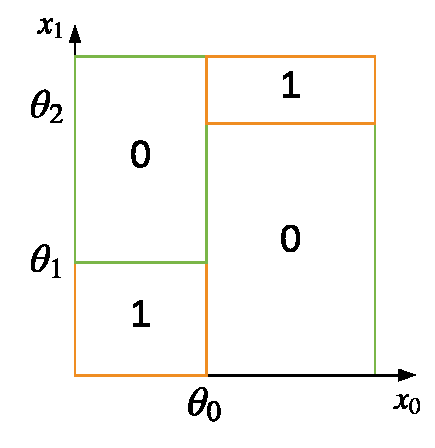
\includegraphics[width=0.5\textwidth,keepaspectratio]{figures/dectree.pdf}
    \caption{Visualization of a 2-dimensional input space being partitioned into 4 regions by a decision tree with its assigned binary labels in each region}
    \label{fig:dectree}
\end{figure}

In this example, the first partition divides the input space into two regions by verifying whether the value for attribute $x_0$ is smaller or greater than $\theta_0$, being $\theta_0$ a parameter learned by the model during training. These two regions are independent after splitting, and thus can be further divided efficiently in parallel. For instance, the region $x_0 <= \theta_0$ is partitioned by comparing if the value of $x_1$ is smaller or greater than $\theta_1$, and since there are no more partitions in this subregion the labels can be assigned. The process is similarly repeated for the region  $x_0 > \theta_0$, where $\theta_2$ was chosen as the splitting point for attribute $x_1$.
 
After the model is trained, it can be easily visualized as a binary tree where each partition corresponds to a node in the tree, and where the leaves contains the identifying labels, which can be seen in \Cref{fig:dectree_bin}. Whenever a new input vector $\mathbf{x}$ is fed to the model, traversing the tree starting from its root will yield a class label in one of its leaves by sequentially navigating through the set of if-else clauses contained at each one of the nodes.  
 
\begin{figure}[h]
    \centering
    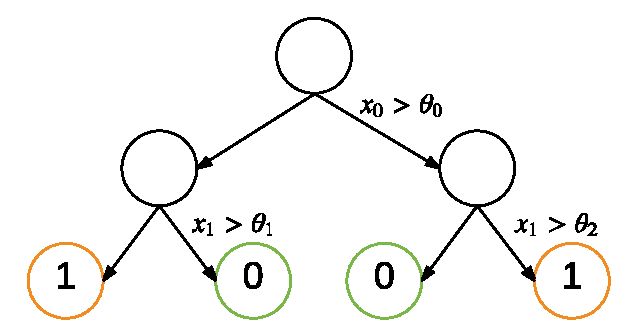
\includegraphics[width=0.6\textwidth,keepaspectratio]{figures/dectree_bin.pdf}
    \caption{Resulting binary tree corresponding to the partitioning performed in \Cref{fig:dectree}}
    \label{fig:dectree_bin}
\end{figure}
 
The learning process of a decision tree corresponds to constructing a binary tree that minimizes the misclassification rate of its training data. That includes finding the optimal number of splits which will define the structure of the tree, and also the values for the splitting coefficients $\theta_i$. To understand how such a tree can be learned, consider a classification problem where $\mathbf{x}$ is a $D$-dimensional vector and $y$ its corresponding class label. The training data is composed of $N$ user vectors forming the $N \times D$ matrix $\mathbf{X} = \{\mathbf{x}_0, \mathbf{x}_1, ..., \mathbf{x}_N,\}$. A tree can be grown by starting at its root and adding nodes sequentially, greedily selecting an attribute and a value to partition the data that minimizes a predefined loss function $H(\mathbf{X})$, which can be performed through an exhaustive search. The set of leaf nodes indexed by $\tau$ represent regions $\mathcal{R}_\tau$ where the prediction labels are assigned.

When decision trees are used for classification, a popular cost function is the \emph{Gini coefficient}, a metric commonly used to measure the statistical dispersion of a population. Let $N_\tau$ be the total number of data points assigned to region $\mathcal{R}_\tau$,  the proportion $p_{\tau k}$ of data points in region $\mathcal{R}_\tau$ assigned to class $k = 0,...,K-1$ such as 

\begin{equation}
p_{\tau k} = \frac{1}{N_\tau} \sum_{\mathbf{x}_n \in \mathcal{R}_\tau} \mathcal{I}(y_n = k)
\end{equation}
 
 where $\mathcal{I}$ is the indicator function. The Gini coefficient can be defined as 
 
 \begin{equation}
 H(\mathbf{X}) = \sum_{k=0}^{K-1} p_{\tau k} (1-p_{\tau k})
 \end{equation}
 
which is minimized whether $p_{\tau k}=0$ or $p_{\tau k}=1$. The Gini coefficient favors grouping high proportions of data points that belong to a single class into each region. The splits are chosen to be the ones that minimize $H(\mathbf{X})$ at each node of the tree, which is why decision trees are considered "greedy" algorithms. The tree can be grown until the reduction of the associated error falls below a predetermined threshold. Empirical observations have shown that pruning back some nodes of the tree after the expansion has finished can improve the performance of the predictor.
 
The decision tree algorithm posses a key property which is one of the reasons why it is so popular: the model can be easily interpreted. The ability to visualize the decision process of the predictive model as a binary tree linked together by a simple set of rules is of great value, and is sometimes deemed crucial in fields like medical science for example. However its largest drawback lies in the fact that decision trees are commonly tightly fitted to the data which they were trained on, and small changes in the input may yield radically different models. This problem, which is known in machine learning as high \emph{variance}, is one the reasons for the creation of the ensemble method in the following section.
 
\subsection{Random Forests}

Random forest is an algorithm mainly used for classification and regression which utilizes an ensemble method for prediction: by training several different and independent classifiers, the predicted class or value can be interpreted as the resulting majority vote from all learners, through a mode or mean function for classification and regression, respectively.

Popularized by Breiman \citep{breiman2001random}, random forests have been used in several different domains, specially for the task of predicting user churn \citep{coussement2013customer} \citep{burez2008separating}. The main principle behind the method is that a group of "weak" learners can achieve a better performance when compared to a single "strong" learner, which can also be interpreted as an implementation of the "wisdow of the crowd". 

In this context, a "weak" learner is a decision tree trained with a subset of the samples and features of the original data. No single tree has access to all input variables, however they predict by casting votes on a class, and the final prediction is the class label which has the majority of the votes.

Each one of the trees is grown as follows:

\begin{enumerate}
\item For a dataset of size $N$, sample $N$ examples from the original dataset with replacement, also known as \emph{bootstraping}.
\item For a dataset containing $F$ features, select $f<<F$ which are the number of features selected at random for building each tree.
\item Grow every tree to its maximum extent, without any pruning.
\end{enumerate}

Suppose that we generate $M$ bootstrap data sets and use each one to train a decision tree $y_m(\mathbf{x})$ where $m=1,...,M$. For a classification problem, $y_m(\mathbf{x})$ outputs the most likely class label $k$, that is the highest $p(k|\mathbf{x})$, for every $k=1,...,K$. The final prediction of the ensemble can be defined as the majority vote of every classifier which is given by

\begin{equation}
y_\textit{RF}(\mathbf{x}) = \underset{k \in K}{\arg\max} \sum_{m=1}^M \mathcal{I}(y_m(\mathbf{x}) = k)
\end{equation}

\subsection{Recurrent Neural Networks}

Recurrent neural networks (RNNs) are a class of artificial neural networks well suited for dealing with data which is sequential in nature. Traditional feed-forward neural networks assume that all input data points are independent of each other, however this can lead to spurious results if this assumption does not hold. For instance, predicting the next word in a text document is tightly correlated with the words that appeared before it. 

Unlike feed-forward neural networks, RNNs allows connections between hidden units, more specifically between the units that are contiguous in time. Updates in a hidden unit in a time step depends on the values in the hidden unit immediately before, and so on until the start of the sequence. While this constitutes a small modification to the classical multilayer perceptron, an important property is obtained in the process: RNNs can in theory map the entire history of previous inputs to each output. 

The memory structure that holds this historical data, hereby called \emph{state}, is the main engine that gives RNNs its predictive power. Consider $\mathbf{h}_t$ and $\mathbf{x}_t$ as the values of the state and input at time step $t$, respectively. The value of state $\mathbf{h}_t$ depends both on the current input $\mathbf{x}_t$ and also the previous state $\mathbf{h}_{t-1}$ as follows:

\begin{equation}
\mathbf{h}_t = \sigma(\mathbf{W}^{xh}\mathbf{x}_t + \mathbf{W}^{hh}\mathbf{h}_{t-1} + \mathbf{b}_h)
\end{equation}

where $\mathbf{W}^{xh}$ is the weight matrix connecting the input to the hidden units, $\mathbf{W}^{hh}$ the weights connecting states time steps $t$ and $t-1$, $\mathbf{b}_h$ the bias vector for hidden unit $h$, and $\sigma()$ the activation function, commonly the sigmoid or the hyperbolic tangent. Values for state $\mathbf{h}_{t-1}$ can be calculated in a similar fashion, until the initial state $h_0$ which is only dependent on the input. This recursive dependence means that an RNN can be "unrolled" through time as to better visualize the interactions between units of the network, which can be seen in \Cref{fig:rnn}.

\begin{figure}[h]
    \centering
    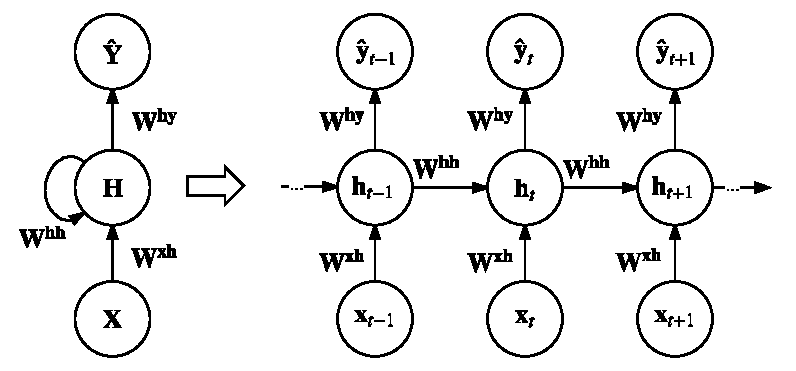
\includegraphics[width=0.7\textwidth,keepaspectratio]{figures/rnn.pdf}
    \caption{A recurrent neural network unfolded through time}
    \label{fig:rnn}
\end{figure}

In a classification problem, the predicted output $\hat{\mathbf{y}_t}$ is a $K$-dimensional vector with the normalized probabilities of input $\mathbf{x}_t$ belonging to the classes $k=1,...,K$, which can be calculated through the following equation:

\begin{equation}
\hat{\mathbf{y}_t} = \phi(\mathbf{W}^{hy}\mathbf{h}_t + b_y)
\end{equation}

where $\mathbf{W}^{hy}$ are the weights connecting the hidden layer to the output, $\phi()$ the softmax function that normalizes its input into probability values, and $b_y$ the bias vector for the output layer. 

\subsubsection{Loss function}

To calculate how effective our prediction is comparing to true labels of the training data, a loss function $\mathcal{L}()$ that computes the distance between true values and the prediction is needed. A common function for a discrete classification problem is \emph{cross-entropy} which calculates the amount of information needed to distinguish one distribution from the other\citep{buja2005loss}, here the predictions $\hat{\mathbf{y}}$ and the true labels $\mathbf{y}$. The equation follows:

\begin{equation}
\mathcal{L}(\hat{\mathbf{y}}, \mathbf{y}) = - \sum_k \mathbf{y}_k \log \hat{\mathbf{y}}_k
\end{equation}

\subsubsection{Initializers}

Any neural network requires a method to initialize its weight matrices $\mathbf{W}$. A common practice is set it to small random numbers centered around zero so the weights can independently learn patterns from the data, which is a better approach when compared to naively setting all values to zero. 

Glorot and Bengio\citep{glorot2010understanding} proposed a method to initialize the weights which is widely adopted in academia, and it goes by the name of \emph{Xavier initialization}. In this method, the values are sampled from a uniform distribution such as

\begin{equation}
\mathbf{W} = \mathit{U}[-\frac{\sqrt{6}}{\sqrt{n_\text{in}+n_\text{out}}}, \frac{\sqrt{6}}{\sqrt{n_\text{in}+n_\text{out}}}] 
\end{equation}

where $n_\text{in}, n_\text{out}$ is the size of input and output layers, respectively. 

Another method to initialize the weights was proposed by Saxe \emph{et al.}\citep{saxe2013exact} by choosing $\mathbf{W}$ to be a random orthogonal matrix such as 

\begin{equation}
\mathbf{W}^T\mathbf{W} = \mathbf{I}
\end{equation}

where $\mathbf{I}$ is the identity matrix. This is called \emph{orthogonal initialization}, and it is a commonly used method for initializing the weights of the recurrent state in a recurrent neural network.

\subsubsection{Regularizers}

A machine learning model is judged to be of good quality if it can generalize well to unseen data. When a model shows good performance during training but fails to achieve the same using test data, the model may have fit all its parameters perfectly to the training set instead of finding a function that explains the data well, a problem which is called \emph{overfitting}. 

A common approach to avoid this complication is to add a term in the loss function that penalizes large values of parameters, which is called \emph{weight decay}. This method favors simplicity by avoiding models that overly complex, which can be considered an application of Occam's razor which states that "among competing hypotheses, the one with the fewest assumptions should be selected". A $L_2$-norm is a regularization that penalizes the parameters by adding the square of the magnitude of the weights to the loss function that we aim to minimize\citep{phaisangittisagul2016analysis}, as follows:

\begin{equation}
\mathcal{L}_r(\hat{\mathbf{y}}, \mathbf{y}, \mathbf{W}) = \mathcal{L}(\hat{\mathbf{y}}, \mathbf{y}) + \lambda \sum_\mathbf{W} |w_i|^2
\end{equation}
 
where $i$ iterates over all available parameters and $\lambda$ controls the fraction of the regularization term that will be added to the loss function.

Another common approach is \emph{dropout}\citep{srivastava2014dropout}, which randomly drop hidden units along their connections during training. This technique acts as a regularization method by removing the units with a probability $p$, avoiding the weights of co-adapting too much. Recurrent neural networks however requires a special implementation of dropout as for it be effective, a topic fully explored by Zaremba and Sutskever\citep{zaremba2014recurrent}.

\subsubsection{Optimizers}

The learning process in an RNN involves finding the set of parameters $\mathbf{W}$ that minimizes the loss function $\mathcal{L}()$. This is accomplished by an \emph{optimizer}, an algorithm that iteratively applies small updates to the weights in the direction where loss function is minimal. A classic optimization algorithm is \emph{gradient descent}, which updates the parameters by computing the gradient of the cost function w.r.t the weights for the entire dataset and moving it in the opposite direction, such as

\begin{equation}
\mathbf{W} = \mathbf{W} - \eta \nabla_W \mathcal{L}(\mathbf{W}) 
\end{equation}

where $\eta$ is the learning rate that controls how much of the gradient will be applied to the weights and $\nabla_W \mathcal{L}$ the gradients. Reading the whole dataset to apply one update to the weights is commonly not feasible due to its computing resources requirements. A more popular approach is to apply updates by looking at a subset of the training samples instead, a process  called \emph{mini-batch gradient descent}.

\begin{equation}
\mathbf{W} = \mathbf{W} - \eta \nabla_W \mathcal{L}(\mathbf{W}; \mathbf{x}^{(i:i+n)},\mathbf{y}^{(i:i+n)}) 
\end{equation}

While mini-batch gradient descent is suitable when the dataset is too large to fit into the memory of a single machine, it has its own set of challenges to solve. First, choosing a proper value for the learning rate might be difficult: low values slows down greatly the convergence process, while large values makes the loss function fluctuate around the local minimum and sometimes even diverging from it. Also, a single learning rate regulates the updates of all parameters, not taking into consideration how sparse the data is and how frequent the features are. It is intuitive to think that weights applied to features that rarely ever are different than zero could have a larger update than the ones that are present in every sample.

To address these problems, new optimizers have been recently introduced. \emph{Adagrad} \citep{duchi2011adaptive} is a gradient-based optimization algorithm that adapts the learning rate dynamically based on the frequency of the parameters. Instead of having a single global learning rate, Adagrad instead has a different learning rate for every parameter of the model, making it suitable for datasets that are sparse in nature. Adagrad updates the learning rate for every weight $w_i$ at time step $t$ by looking into the previous gradients that have been calculated for it, as follows

\begin{equation}
w_{i,t} = w_{i,t-1} - \frac{\eta}{\sqrt{\mathbf{G}_{ii, t-1} + \epsilon}} \nabla_w \mathcal{L}(w_{i,t-1})
\end{equation}

where $\mathbf{G}_{t-1}$ is a diagonal matrix containing the sum of squares of the gradients for parameter $w_i$ up until time step $t-1$, and $\epsilon$ a smoothing parameter.

Another optimization algorithm that aims to smartly adjust the learning rate based on the parameters is called \emph{Adadelta}\citep{zeiler2012adadelta}, which is an extension of Adagrad that more efficiently makes use of the stored past gradients. Instead of storing every gradient into matrix $\mathbf{G}$, a fixed sized time window is set, which is used alongside a decaying average function over the past squared gradients in the window, such as

\begin{equation}
\begin{aligned}
\mathbf{E}[g^2]_t &= \gamma \mathbf{E}[g^2]_{t-1} + (1-\gamma)g^2_t\\
w_{i,t} &= w_{i,t-1} - \frac{\eta}{\sqrt{\mathbf{E}[g^2]_t + \epsilon}} \nabla_w \mathcal{L}(w_{i,t-1}) \\
\end{aligned}
\end{equation}

where the running average $\mathbf{E}[g^2]_t$ depends on a fraction of the previous average and the current gradients. A similar unpublished approach that was developed independently and presented in a Coursera lecture by Hinton is \emph{RMSProp}\citep{hinton2012rmsprop}, which will also be used in this project. 

But how are the gradients calculated in a recurrent neural network? This is accomplished through the \emph{backpropagation through time} (BPTT) algorithm introduced by Werbos \citep{werbos1990backpropagation}. The method is an extension of the standard backpropagation algorithm of feed-forward neural networks, where the gradient calculated at time step $t$ is propagated back to the previous time steps until the start of the sequence $t_0$. The reader is invited to refer to Werbos' paper for details of its implementation.

\subsubsection{Vanishing and exploding gradients}

Even though theoretically RNNs can be used to map input and output sequences of an arbitrary size, in practice learning from long-range dependencies poses a challenge that is difficult to overcome. This is due to a problem called \emph{vanishing and exploding gradients} explored by Bengio \emph{et al.} \citep{bengio1994learning} and extended by Hochreiter \emph{et al.} \citep{hochreiter2001gradient}. Neural networks learn by updating the parameters by a proportion of the gradient of the error function w.r.t the current weights, and this process can be made difficult either if the gradients go to zero (no learning at all) or explode to large numbers (missing the local optima at every turn). In RNNs and also other deep architectures, the top layers may fail to learn in an adequate pace since its update is backpropagated through the bottom layers by multiplying the intermediate gradients through the \emph{chain rule}. If those gradients are consistently between -1 and 1, which is the case of the most common activation functions, through the chained multiplication of the derivatives the weight update of previous layers will quickly approach zero. Other activation functions like the Rectified Linear Unit $max(0,x)$ may instead make the gradients increase rapidly due to its constant derivative of 1 w.r.t $x$ for every value greater than 0.

Some solutions have been proposed to tackle this complication. A well-known variant of the learning algorithm of RNNs is the \emph{truncated backpropagation through time} (TBPTT) which aims to solve the exploding gradient problem for continuously running networks \citep{williams1989learning}. In it, one can set a maximum number of time steps alongside which error can be propagated. Using a small cutoff value would alleviate the problem of gradients increasing too fast, however at the cost of learning long-range dependencies. A more modern approach however carefully design the nodes as to avoid the vanishing and exploding gradients problem while also being able to learn from information hidden long back in the input sequence, which shall be explored in the following section.

\subsection{Long Short-Term Memory}

The long short-term memory network is an extension of a RNN that can extract long-range dependencies from the sequential input without suffering from the negative consequence of the vanishing and exploding gradients common in deep architectures. Firstly proposed by Hochreiter and Schmidhuber \citep{hochreiter1997long} and further extended by Gers and Schmidhuber \citep{gers1999learning}, this technique has recently been applied successfully for domains like speech recognition \citep{graves2013speech} and video classification \citep{yue2015beyond}.

The main property that differentiates LSTMs with its counterpart is its \emph{memory cell} which controls the flow of information that goes from the input $\mathbf{x}_t$ to the hidden states $\mathbf{h}_t$. This is accomplished by using a unique \emph{cell state} variable $\mathbf{s}_t$ which contains the global information that the network currently has about the input sequence, which can be seen as its "memory". A visualization of the memory cell and its traversing state variable can be seen in \Cref{fig:lstm}.

\begin{figure}[h]
    \centering
    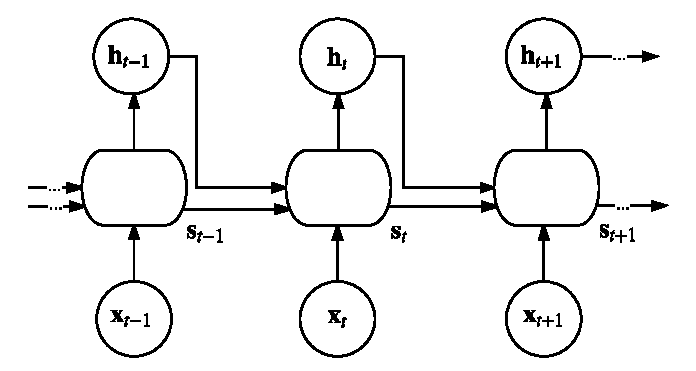
\includegraphics[width=0.7\textwidth,keepaspectratio]{figures/lstm.pdf}
    \caption{A LSTM network unfolded through time, with the oval shaped structure as the memory cell}
    \label{fig:lstm}
\end{figure}

The memory cell structure of a LSTM is responsible for updating the cell state at each time step. This is accomplished by a set of so called \emph{gates} that controls how the information will get in and out of the cell state. A modern LSTM architecture is composed of three of these gates, hereby called \emph{input}, \emph{output} and \emph{forget gates}, alongside the \emph{input node} which is a transformation over the raw input sequence. 

One can intuitively think of LSTM gates as controllers whether the activation for a given unit is let in and out of the cell state at each time step, which can be learned during network training. During the forward pass, if the input gate is zero, no activation can get into the cell state. Similarly, the output gate learns when it should let the activation leak out of it. The forget gate being equal to zero erases all the memory previously stored on the cell state, basically forgetting what was learned in the past. During the backward pass phase, the gradient may propagate several time steps in the past without exploding or vanishing due to its constant error carousel. Through this angle the memory cell learns as to when it should let the error in and out of the cell state.

A LSTM memory cell at time step $t$ is fully described by the following set of equations:

\begin{equation}
\begin{aligned} 
\mathbf{g}_t &= \sigma_g(\mathbf{W}^{xg}\mathbf{x}_t + \mathbf{W}^{gh}\mathbf{h}_{t-1}+\mathbf{b}_g) \\ 
\mathbf{i}_t &= \sigma_i(\mathbf{W}^{xi}\mathbf{x}_t + \mathbf{W}^{ih}\mathbf{h}_{t-1}+\mathbf{b}_i) \\
\mathbf{f}_t &= \sigma_f(\mathbf{W}^{xf}\mathbf{x}_t + \mathbf{W}^{fh}\mathbf{h}_{t-1}+\mathbf{b}_f) \\
\mathbf{o}_t &= \sigma_o(\mathbf{W}^{xo}\mathbf{x}_t + \mathbf{W}^{oh}\mathbf{h}_{t-1}+\mathbf{b}_o) \\
\mathbf{s}_t &= \mathbf{g}_t \odot \mathbf{i}_t + \mathbf{s}_{t-1} \odot \mathbf{f}_t \\
\mathbf{h}_t &=  \sigma_h(\mathbf{s}_t) \odot \mathbf{o}_t
\end{aligned}
\end{equation}

where $\mathbf{i}_t, \mathbf{o}_t, \mathbf{f}_t$ are the input, output and forget gates, respectively. $\mathbf{x}_t, \mathbf{h}_{t-1}, \mathbf{s}_{t-1}$ are the input vector at the current time, and the hidden units and cell state from the previous time step, which are the inputs to the memory cell. $\mathbf{W}, \mathbf{b}$ are the weight matrices and the bias vectors for each gate and node. $\mathbf{g}_t$ is the input node. $\sigma$ are the activation functions: modern architectures use $\sigma_g,\sigma_h$ as the hyperbolic tangent function, whereas $\sigma_i,\sigma_f,\sigma_o$ as the sigmoid \citep{zaremba2014learning}. The output of the memory cell are the updated cell state $\mathbf{s}_t$ and hidden units $\mathbf{h}_t$.

Networks that makes use of the memory cell structure of an LSTM have been shown to outperform classical recurrent networks by being able to learn long-term dependencies from the sequence in a more efficient way. Positive results were obtained both in artificial datasets carefully designed to test the ability of the network learning long-term dependencies \citep{bengio1994learning} and more recently in demanding sequence processing tasks \citep{graves2013speech}\citep{sutskever2014sequence}.

\section{Linear Dimensionality Reduction}

Principal component analysis (PCA) is a widely used method for applications like data compression, dimensionality reduction and data visualization. Initially invented by Pearson\citep{pearson1901liii} and later independently developed and named by Hotelling\citep{hotelling1933analysis}, PCA strives to find an orthogonal projection of the original data into a lower dimensional space (also known as the principal subspace) where the variance of the projected data is maximized.

Consider a dataset composed of $N$ samples, each one being $D$-dimensional vector $\mathbf{x}_n$, and also a $D$-dimensional unit vector $\mathbf{u}$ where the samples are going to be projected on. The goal of PCA is to find a projection into a $M$-dimensional space where $M < D$ and where the variance of the projected observations are maximized, which can better be visualized in \Cref{fig:pca}.

\begin{figure}[h]
    \centering
    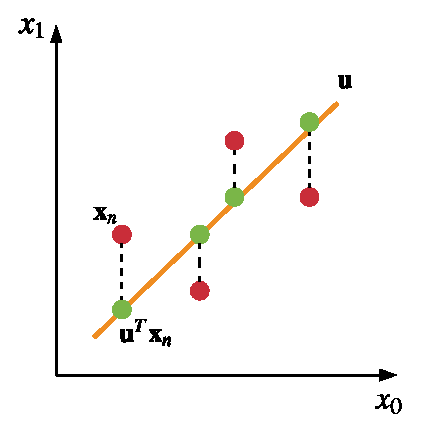
\includegraphics[width=0.5\textwidth,keepaspectratio]{figures/pca.pdf}
    \caption{An example of PCA reducing the dimensionality of the data}
    \label{fig:pca}
\end{figure}

After projecting the observations into the unit vector previously defined and obtaining $\mathbf{u}^T\mathbf{x}_n$, the variance of the projected data can be calculated with the following set of equations:

\begin{equation}
\begin{aligned}
\mu &= \frac{1}{N}\sum_{n=1}^N \mathbf{x}_n \\
\Sigma &= \frac{1}{N}\sum_{n=1}^N (\mathbf{x}_n - \mu)(\mathbf{x}_n - \mu)^T \\
\mathbf{V} &= \frac{1}{N}\sum_{n=1}^N (\mathbf{u}^T\mathbf{x}_n - \mathbf{u}^T\mu) = \mathbf{u}^T\Sigma\mathbf{u}
\end{aligned}
\end{equation}

where $\mu$ and $\Sigma$ are the mean and the covariance matrix of the sampled data, respectively. Maximizing the value of the variance $\mathbf{V}$ with respect to $\mathbf{u}$ is an optimization problem constrained by $\mathbf{u}^T \mathbf{u}=1$. Hotelling\citep{hotelling1933analysis} shows that by introducing a Lagrange multiplier $\lambda$, this can be turned into an unconstrained optimization where

\begin{equation}
\mathbf{u}\Sigma\mathbf{u} = \lambda_1
\end{equation}
	
and so the variance will be maximized by picking the eigenvector corresponding the largest eigenvalue $\lambda_1$, which is known as the first \emph{principal component}. The following $M-1$ principal components can then be chosen sequentially by picking the vector which is orthogonal to all other principal components already considered, which is equivalent to choosing the eigenvectors corresponding to the largest $M-1$ eigenvalues $\lambda_2,..., \lambda_M$.

\chapter{Related Work}
\label{cha:related_work}

There is considerable amount of work done on the churn prediction realm. The most common topic that is addressed by the literature is evaluating different types of predictive models trained on a domain-specific dataset, like the telecom and financial industries for example. Understanding what techniques are commonly used on the field is deemed crucial for the success of any churn rate predictive model.

The use of data represented as a time-series for predicting churn, although of high interest to this project, is a rather under researched topic as of today, the user features being commonly aggregated over a time window on the whole observation period. Recently though some interest has been sparked on the literature about trying to leverage temporal aspects of the user behavior by representing the data as a sequential input, and some examples similar to the task at hand, while not abundant, can nevertheless be found. 

Other research papers focus on answering how different properties inherent to the churn prediction problem affect the performance of classifiers, like for example how to deal with unbalanced data sets, how the evaluation procedure should be performed and how far back in the user history should models be trained on as to obtain a proper balance between accuracy and processor usage.  

This chapter will introduce the literature on the fields of interest for this project, and will focus mainly on the following topics:

\begin{itemize}
\item Identifying the state-of-the-art for training, modeling and evaluating churn predictor classifiers, the algorithms being used, the methodology for the experiments and the observed results.

\item Researching current techniques for creating models that leverage the properties of time-series data, applied for churn prediction (if any) or similar domains where we can map our problem to. It shall also be studied common features of sequential data as to better understand how to best exploit its properties as to improve the accuracy of our models.

\item Understanding prevalent characteristics on data sets used for churn prediction as to improve the performance of models and also to avoid common pitfalls when training and evaluating their accuracy.
 
\end{itemize}


\section{Churn Prediction}

Identifying which users are most likely to churn is an important step in any customer relationship management (CRM) framework interested in improving user retention. It has been shown that several economical values are directly correlated with the customer lifetime metric that can be crucial in a competitive market, like how the costs of acquiring new customers surpass those of retaining existing ones and how loyal users usually spend more and can bring in new customers \citep{GurAli2014}. Thus, churn rate prediction is an established topic in the literature and has seen studies being performed on a wide range of domains like the telecommunication industry \citep{Lu2014}\citep{Khan2015}\citep{Hassouna2015}, social multiplayer games \citep{Borbora2011}\citep{Runge2014} and community-based question answering services (CQA) \citep{Pudipeddi2014}\citep{Dror2012}. 

The very first aspect of the study that any researcher has to take into consideration is the formal definition of what churn is, which depends on the domain that the data set belongs to. \citep{lazarov2007churn} divides the definition into three types: \emph{active} where the contract is officially terminated, \emph{hidden} when the customer is inactive (not using the service) for a significant amount of time, or \emph{partial} when the customer is not using the service at its fullest, opting for a competitor instead. Subscription-based services like mobile companies \citep{Lu2014}\citep{Hassouna2015} and massive multiplayer games \citep{Borbora2011} commonly utilizes the active churning definition caused by the explicit termination of the agreement. Social games \citep{Runge2014}\citep{Drachen2016RapidPO} and CQA services \citep{Pudipeddi2014}\citep{Dror2012} however usually model the user interest by measuring its level of activity and engagement since no contract is formally established, opting for the hidden churn definition instead. 

Even though the service provider has a contract-based paid product, this project is interested in the clients who are inactive for some time, whether they are paying customers or not. Delving into the hidden churn definition, one could ask what is considered a "significant amount of time" as to judge a user to have churned or not, and different domains have distinct approaches depending on the way the interaction between user and service takes place. For example, for a mobile network like the one studied in \citep{Khan2015} this definition can span months of inactivity since customers on that market are commonly more loyal, even though this paper focus on pre-paid accounts with "soft" contracts. On the other hand, rapid-changing markets like free-to-use services as social games and CQA sites prefer to define the churn period as small as possible (commonly days or weeks), since the absence of an agreement makes it easy for customers to switch for the competition, having the service the obligation to act faster if any sign of loss of users is identified \citep{Khan2015}\citep{Drachen2016RapidPO}. On \citep{Dror2012} the focus is set on new users so the the churn period is explicitly set to be their first week of activity. \citep{Pudipeddi2014} however focus on both new and experienced users by considering the first days and posts (questions and answers) as parameters on the models trained, evaluating each independently.

Current literature for prediction of churn rate uses a wide range of machine learning technologies, such as decision trees \citep{Pudipeddi2014}\citep{Hassouna2015} \citep{Ballings2012} \citep{Khan2015}, logistic regression \citep{GurAli2014}, neural networks \citep{Runge2014} and its convolutional variant \citep{Wangperawong2016}, random forests \citep{Dror2012} and support-vector machines \citep{coussement2008churn}. The number of techniques is vast, however it can be mentioned that current research suffers from a difficulty to reach insights that can generalize well for other areas, since the applications that the data sets belong to are domain-specific, greatly influencing how the users interact with the service. Interpretability is a key component in any application since the end goal is always not only to detect the users most likely to defect but also the reasoning behind their departure, as to plan reasonable actions to increase retention. With that in mind, even though some models like weighted random forests \citep{Burez2009} and neural networks \citep{Runge2014} offer a higher accuracy for some domains, the difficulty in getting key drivers behind the consumer's behavior in some "black-box" type of models have led to researchers opting for a more interpretable technique like logistic regression which is commonly a close second place in terms of performance \citep{Runge2014} \citep{Dror2012}. For that reason, decision trees and logistic regression are as of today the most popular techniques for churn prediction, yet a consensus of the best model cannot be reached by researchers as stated by \citep{mahajan2015review}. 

The telecom industry is by far the most well researched area for predicting churn, and a proper review would be incomplete without mentioning some examples. In \citep{Hassouna2015}, two popular models for predicting user churn were empirically compared: decision trees and logistic regression. By making use of the data set provided by a mobile operator, two models were created by independently training and selecting their best performing versions. Evaluation was executed by comparing the area under the curve (AUC) of their receiver operating characteristic (ROC) curves, as also their Lift score and overall accuracy. The conclusion is that decision trees consistently perform better when compared to logistic regression models, and thus should be a preferred choice. In \citep{Lu2014}, churn classification was performed on users in a rather unique way. The Gentle AdaBoost boosting algorithm was used alongside a logistic regression base learner as to train a model to do the separation between the churning and non-churning classes. However, one further step was performed where the users were split into two clusters based on the weights assigned by the boosting algorithm. One of the clusters was identified to have a considerably larger churn rate than the other, and thus another logistic model was trained using the clusters as labels, and its performance evaluated using ROC curves. The idea behind this approach is to use a model to mark users who have a high risk of leaving the service (and be the focus of user retention actions), instead of labelling them as churners and non-churners directly. On \citep{Khan2015}, billions of call detail records from a mobile phone operator was the focus of a churn prediction study and feature analysis. The initial data set was filtered to the calls made by 100.000 subscribers during a 6 month period. A brute-force approach to feature engineering was then performed to create 12.914 out of the initial 10 features by combining every feature from each of the manually split 8 different groups. Feature selection is then performed in two distinct ways: first, an individual Student's t-test score is computed for each individual feature to evaluate how well it can differentiate between the churners and non-churners sets. Second, a tree-based method was used as to estimate the the accuracy of a joint classifier by adding features one at a time. Features are then ordered by their statistical correlation with churn, and the top 100 features were selected to train several different classifiers. Evaluation was performed mainly by comparing the AUC of each model, where AdaBoost using a decision tree classifier performed the best, followed closely by a logistic regression model.

The rapid increase in Internet popularity has spawned a plethora of new services in the last decade, and thus a wider range of domains like CQA sites and gaming applications are being researched for churn prediction. In \citep{Dror2012}, an explorative study was made on the Yahoo! answers website as to discover an efficient churn predictive model and also the features that correlates with the user leaving the service, however differently from other works this paper focused on new users with less than a week of activity on the service. Features were grouped into Question, Answer and Gratification categories, and were used for training several different classifiers. For this dataset, random forests performed the best with logistic regression as close second. Features were also ordered by the amount of information gain that they provide, and the number of questions and answers are the top features on that regard (inversely correlating with churn), followed by the period of time the user is active and gratification features for answers given and questions made. In \citep{Pudipeddi2014}, the younger CQA service Stack Overflow was the focus of a study on user behavior characterization and churn rate prediction. An extensive data exploration was made as to correlate features to the chance of a user leaving a service, and with those insights classical modeling techniques were used, where the best performing one was a decision tree. The approach used for extracting and categorizing features (temporal, frequency, gratitude, etc) and the insights that follow the study (like the importance of temporal features for predicting churn) is of high value and can be mapped to concepts on a different domain like a music streaming service with minor modifications. 
In \citep{Runge2014}, players responsible for generating the most profit on two casual social games were the focus of a study on churn analysis and prediction. Formal definitions for active players and churning were made, and the problem was defined as a binary classification task where users were labelled as leaving the service or not in the following week of when the models were trained. Four different models were then trained, and a neural network classifier obtained the best AUC score, with logistic regression as a close second. The formal definitions of "churn" and "activity" can be applied to a music streaming service in a similar way, as the evaluation of performance using a series of ROC curves. In \citep{Borbora2011}, the activity log of a subscription-based multiplayer online game was the source of an experiment focused on comparing two different methods for predicting the users with a higher tendency to leave the service, a theory-driven and data-driven approaches. For the modeling, an ensemble method was used with several different classifiers, where the choice of model was made based on whether the cluster of the data set (found with K-means) that will be used to train the classifier has a significant proportion of churners or not. Even though the performance of the data-driven model was superior, the difference was negligible when taking into consideration the complexity of the models and also its interpretability. Moreover, if marketing resources are constrained the theory-driven model was considerably superior for the first 40\% of users on the lift chart. 


\section{Sequential Modeling for User Behavior Data}

Even though there is currently a wealth of research on churn prediction techniques, most of them treat the user behavioral features as static points in time by aggregating or summarizing their values over a time window \citep{Auon2015}. It is a simplification that eases the hassle of training models with a data set which is commonly high-dimensional and difficult to work with, however information that could be used to improve the predictors' performance is lost in this process  \citep{GurAli2014}. For example, there is no information as to when over the time window being analyzed a user decides to churn, it could be that all defectors are grouped into a period where an external event (like the end of an offer) has taken place. Environmental variables, that is those that varies through time but are common to all users, are also omitted on static models, leaving it to the experts the task of manually integrating these features on their analyses. Newer models like \citep{Pudipeddi2014} attempt to integrate some temporal data by manually engineering features related to time (like the duration of an event, for example), however since each user is represented as a sample in a single point in time the sequence of data transformations is inherently lost in this process.

It is natural to think that the human behavior evolves through time. Our opinions and desires changes in accordance to the stimuli that we receive from the world around us, and summarizing our persona by looking at a single point in our life is an oversimplification that does not make justice to the path that leaded us to where we are. Dealing with temporal data is by no means trivial however, and to leverage fully its properties some careful considerations about this type of data must be done. On \citep{Langkvist2014}, an overview of the challenges on creating models that make use of the time component on data sets are presented to the reader. Also, since hand-crafted features are generally domain-specific and difficult to create, a review of the current research on unsupervised feature learning applied for time-series data is the focus of this paper. From the challenges, it is worth of mention the uncertainty that there is enough information to understand the underlying process, its non-stationary characteristics like mean, variance and frequency, and its common high dimensionality and noise. The right representation is deemed then crucial for any model to be successful in its goal. Several different techniques currently being used for unsupervised feature learning are then presented in details to the reader, where it is worth of quick mention the conditional Restricted Boltzmann Machine (cRBM), Recurrent Neural Networks (RNN, with is Long Short-Term Memory extension), the Gated RBM, the Time-Delay Neural Networks, and the Space-Time Deep Belief Network. Finally, several classical time-series problems are reviewed alongside the best models currently being used for each domain. 

The hypothesis that sequential patterns hidden on temporal data can improve the accuracy of predictive models is not an uncharted territory however, and has being recently explored by researchers on similar domains as churn prediction that could be mapped to with minor modifications. Sparked by positive results of recurrent neural networks on domains like speech recognition \citep{graves2013speech} and video classification \citep{yue2015beyond}, some papers attempt to recreate similar deep architectures on their own prediction problems. On \citep{Tax2016}, a technique was presented as to predict the next event and its timestamp on a running case of a business process (a help desk process, for example). Three different LSTM architectures were experimented on, one for each of the problems being tackled: estimating the next activity and its timestamp, all the remaining activities in a use case and the remaining time of a process. This technique could be used for churn prediction by interpreting the user interaction with the service as actions, and "churn" could be an event that may or may not exist in the process chain. The LSTM architecture was also present on \citep{Auon2015} alongside a quantile regression (QR) model as to predict which of the past buyers of a store chain will return after acquiring a product on sale. The hypothesis is that a performance gain can be achieved by combining models that are know to perform well on both temporal and aggregate features, respectively. It was empirically shown that a mixture of experts approach between these two techniques can reach a significant mean-square error improvement when comparing to any of the models when evaluated independently. 

Deep architectures like LSTMs could theoretically be applied in a similar way for the task of predicting which users are more likely to abandon a service, however the lack of research using techniques like these suggests that this mapping may not be as easy as it seems, nevertheless some examples can still be found in the literature. Inspired by results obtained on image recognition \citep{krizhevsky2012imagenet}, a convolutional neural network (CNN) model was used as a churn predictor on the work by \citep{Wangperawong2016}. On it, users were represented as 2-dimensional images where columns are the tracked features and rows are days organized in sequences. Two different CNN models were used, and both outperformed a baseline decision tree model. On \citep{GurAli2014} the researchers propose a new data set generation framework that can better leverage the temporal aspect of user behavior data for churn prediction models. The hypothesis being tested is that by boosting the data with features on different time periods instead of only the last one, a significant performance gain can be achieved. The main framework of this study is called Multiple Period Training Data (MPTD), which basically consists of aggregating to each user their features at each predefined time step along the time range of the data set, alongside their churn labels at each point in time and also environment variables which varies through time but are common for all users. This framework was tested against a classical static data set, demonstrating a significant improvement (by \emph{p-value} comparison) on AUC and top decile lift (TDL) for both logistic regression and decision tree models for predicting if the user is going to churn on the next test period or nor. Another experiment was focused on predicting churn several periods on the future, and for that a common survival analysis method called Cox regression was used as a benchmark for comparison against logistic regression models trained on MPTD. It was empirically concluded that using several independently trained binary classifiers, each trained on a different parameter to the "churn within $\delta$ periods" (W$\delta$C) feature, a significant performance gain can be achieved when comparing their respective AUC and TDL.


\section{Evaluating and Training Churn Prediction Models}

Data sets from service industries often have a common characteristic that may be problematic while training models, which is the uneven distribution between the churning and non-churning classes. It is a common scenario for the number of non-churners to heavily outweigh the number of churning samples on real data sets. Class imbalance is thus a recurrent concern in almost all domains, however research in this area lacks the proper attention. \citep{Burez2009} aims to solve this mystery by focusing entirely on how the uneven class distribution affects the performance of several different classifiers. The performance boost estimated to be received by using a cost-sensitive learning algorithm (where false negatives are assigned a greater cost than false positives) is also evaluated, and it has taken the form of a weighted random forest model which was compared to other classical baseline models like logistic regression and random forests. Under-sampling, where fewer samples from the majority class are incorporated in the training data as to artificially change the distribution between the labels, is proved to significantly improve the performance of the underlying models, however the exact ratio between churners and non-churners is confirmed to be case-dependant, not necessarily being the even distribution the perfect choice. 

To deal with the problems brought by the unbalanced distributions mentioned above, proper evaluation metrics must be used as to avoid the predictors to be biased towards the majority class. It is a well know fact that the accuracy of a classifier is not an appropriate method when comparing the performance of different models \citep{powers2011evaluation}, and so no paper reviewed used this metric by itself. The overwhelming majority of the literature abides by the use of AUC as a proper metric for predicting churn rate, \citep{Ballings2012} \citep{GurAli2014} \citep{Khan2015} \citep{Lu2014} to name a few. \citep{Burez2009} delves into this topic and defends the use of AUC as a proper metric, while adding the cumulative gains chart as to graphically represent the percentage of customers has to be targeted to reach a percentage of churners. The F-score is also sometimes added as a metric of interest, normally in conjunction with AUC \citep{Dror2012} \citep{Khan2015}. In respect to graphical representations, ROC curves and lift charts dominates the literature as appropriate methods, and it is present in works like \citep{Lu2014} and \citep{Burez2009}. 

Another question that can be made is how far in the user history models must be trained on as to achieve the best trade-off between accuracy and computational burden. It is intuitive to imagine that user actions far in the past exerts little influence on predicting whether the user is going to churn or not in the near future, however the exact threshold that should be used is not trivial to find. \citep{Ballings2012} attempts  to answer this question by experimenting with three different models (logistic regression, decision trees with and without bagging) on a newspaper data set consisting of 16 years of user history. The models were evaluated for their performance by training with data ranging on this interval with a 1-year gap between each measurement. It has been concluded that  after year 5 no gain in performance (measured by AUC) is statistically relevant enough to warrant the increase in computational power needed for the training. However, the researchers also question whether this result can be extended for other domains or not, leaving that for future work.

Current data sets from service providers have no lack of user historical information stored, however the probability that all available features have a significant correlation to churn rate is slim. Using too many features may lead to undesirable effects like overfitting and falling into the "curse of dimensionality" problem, reducing the classifiers performance as cited by \citep{guyon2003introduction}. It is a common step to pre-process the data in a way as to mitigate this risk, but still there is no single method in the literature that dominates the scene. Several papers do a manual subset selection of features based on theories, testing each using baseline classifiers and selecting the subset with the best performance \citep{Pudipeddi2014}\citep{Runge2014}. Others works like \citep{Borbora2011} and \citep{Dror2012} use information gain as a metric to classify the features on their expected reduction in entropy. One step further is taken by works like \citep{Lu2014} and \citep{Khan2015} where full decision trees are built specifically for feature selection. Another more exotic method was used by \citep{Wangperawong2016} with an autoencoder to discover which features influenced the churn rate the most. 

\chapter{Dataset Creation and Exploration}
\label{cha:data}

\epigraph{In God we trust: all others bring data.}{\textit{William Edwards Deming}}

Creating a dataset that is suitable for predicting churn is far from being a trivial task, mainly due to the large amount of information available regarding user behavior. This chapter will be dedicated to delving into details on how the dataset used for training our models was generated, how the sampling was performed, which features were chosen and engineered, and also exploring it in details.

\section{Infrastructure and Data Sources}

Every time a user streams content owned by the service provider, a log entry measuring the user experience and interaction with the product is generated. This information can be the feature of the application used on this stream, its length in miliseconds, the context in the app where this stream originated from, to mention a few. A data pipeline aggregates the collected data into massive datasets hosted on a cloud provider. After processing and cleaning procedures, the provider generates a set of tables containing streaming information of its customers, which sums up to billions of rows per day. 

\section{Dataset Creation}

Extracting relevant data in this scale, and building a dataset that represents the target population for this study has been one of the most challenging parts of this work. While it is desirable to train models with all the data that is available to us, doing so is an engineering feat by itself that could span the entirety of a project. Thus, we need to make smart decisions as to create a dataset that is representative of the audience while also avoiding scalability pitfalls that may occur when working with big data.

In this section, the \emph{data pipeline} used for building the dataset used for model training and evaluation will be presented, which can be seen in \Cref{fig:pipeline}. Each subsection corresponds to a stage in the pipeline, while the source is stream information provided by company and the output is the dataset in a format suitable for model training.

	\begin{figure}[h]
    \centering
    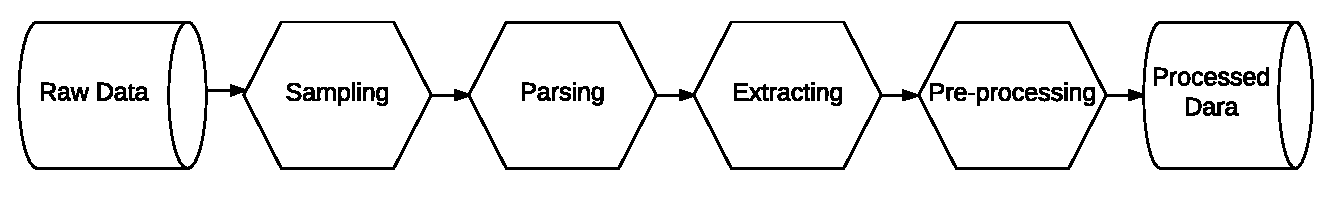
\includegraphics[width=0.9\textwidth,keepaspectratio]{figures/pipeline.pdf}
    \caption{Dataset creation pipeline}
    \label{fig:pipeline}
	\end{figure}

\subsection{Sampling}
\label{sec:sampling}

Each day hundreds of terabytes of streaming information are collected through the provider's data pipelines, aggregating customer usage of the application over several different platforms and countries. Since it is out of the scope of this project to train models with the data in its entirety, one of the challenges will be to understand the information that is available to us and to choose a subset of samples that are representative of the target population that we intend to focus on in this study. This task can be daunting by itself, so this project will make use of previous studies performed by the service provider as a guidance on which samples to choose.

The main rule applied for sampling users is by filtering those who have at least one stream of significant length during the activity window described in \Cref{sec:timewindows}. By applying this filter, we make sure that the users were active right before the period of prediction. Thus, users marked as churning did so between the period of observation and prediction, and we guarantee that we are not choosing samples who churned a long time ago.

Selecting users that created accounts any time during the observation period might skew our models towards a level of inactivity that does not corresponds to reality. For example, if a new account was created right by the end of the observation window, we might erroneously assume that the user was inactive for all days before the registration date. To avoid this, only users that registered into the service any time before the observation starts are sampled into our dataset. 

The service is provided through a wide range of devices. To minimize the influence that different platforms may have on predicting churn, we only look at user experience on one mobile platform. 

After all the previously mentioned filters, we apply the final selection of customers by using a sampling algorithm, resulting in a grand total of \emph{414794 users} in the dataset. Their streams were gathered through the course of 86 days (the standard size of the time windows), summing up to more that a billion streams. This was only made possible by making use of the vast amount of computational resources available for this project, and also through well-known distributed frameworks like Spark and BigQuery. 

\subsection{Parsing}

The source of a stream can come from different \emph{streaming contexts} in the service. Examples of context are personalized content tailored around user taste, editorial content based on popular sets, and the user's own created list of media. Each stream originates from a certain context of the application. Previous studies from the provider indicates that there is a non-zero relationship between the most commonly used context that a user's streams originates from and its probability to churn, thus we add this information in our own dataset. A sample of streaming contexts follows:

\begin{itemize}
  \item \verb|personalized_content| A stream originated from a list of media created by the service provider and personalized to the user.	
  \item \verb|user_content| A stream from a list of media content manually created by the user.
   \item \verb|editorial_content| A stream from a list of content created by the editors of the service provider.
\end{itemize}

This stage of the pipeline extracts the context information from each stream and generates attributes that will be used in later stages to create new features. The sheer amount of data available in our dataset makes it impractical to iterate over the streams and apply a extraction method sequentially over the streams. Thus, we instead make use of a batch-processing programming models that are specialized in processing large datasets. 

\subsection{Feature Extraction}

After filtering the group of streams from the users that we are interested in and parsing the streaming context information, the process of extracting and engineering the features can be started. The main goal of this stage is to create the sequential dataset that is going to be used for training the temporal models, while also calculating the binary labels that will indicate whether the users are going to churn or not. Before introducing the resulting features however, understanding how the time range was divided into different windows is utmost importance as to better comprehend how these features are generated.

\subsubsection{Time Windows}

In order to predict whether a user is going to churn in the future or not and generate the churn binary labels, the time sequence is split into two time windows. The \emph{observation window} is the time span where the user behavior is tracked, data which will be used for training the predictive models. It is sequentially followed by a \emph{prediction window} that is exclusively used for generating the churn label. The windows can be better visualized in \Cref{fig:timewindows}. In order to make sure that selected users did not churn a long time before being observed, the last few days of the observation window are used for sampling users who are active, a time span called \emph{activity window}. 

The size of each window is a parameter that shall be experimented on, but a standard length of \emph{56 days} for the observation window, \emph{30 days} for the prediction window and \emph{3 days} for the activity window were chosen by the provider as values that are suitable for the task at hand. This encompass user information gathered from March 5th until May 29th, 2017. Unless otherwise stated, there are going to be the values in use for our experiments.

The user is considered to have churned if he has at least one active stream during the activity window, but no stream during the prediction window, which follows the definition of "churn" from \Cref{sec:timewindows}. An important factor that should be mentioned is that every user will have a single label for the whole sequence, and not a different label per point in time. This can be considered a simplification that reduces the complexity of our predictive models, however it fails to capture users that change between "churned" and "retained" states often: a user that churned may return to the service given more time. Changing the labeling method will be briefly explored in \Cref{sec:future_work}.

Our source dataset is sequential by nature. Taking this data as it is however is unsuitable to be used for training since commonly temporal models requires that (a) the time step between events to be constant and (b) it possess the same number of samples in every time step. Since there is no control as to when any given user will interact with the application, some data transformations must be performed. 

First, a constantly-sized \emph{time step} was chosen as to split the observations equally across time. To capture the routine of users between every day-night cycles, a time step of 8 hours was deemed to be a suitable value. The features of users are then aggregated over this time range through a mean function. 

Second, the features of users that have no streams in any single time step are set to zero as to keep the number of samples constant through time. This processing will result in a dataset which is quite sparse, since rarely ever a user streams content in all 8 hours time spans over the course of 56 days of observation. An example of this processing can be seen in Figure \ref{fig:zerofill}.

	\begin{figure}[h]
    \centering
    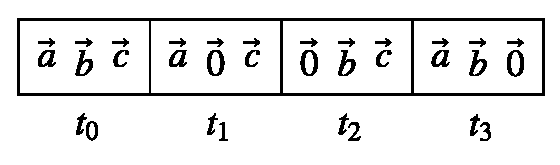
\includegraphics[width=0.8\textwidth,keepaspectratio]{figures/zero_fill.pdf}
    \caption{Zero-filling 4 time steps for 3 different users}
    \label{fig:zerofill}
	\end{figure}

After applying the previously mentioned transformations, the number of rows of the dataset is reduced to \emph{87 million}, each one corresponding to a 8 hours aggregated time step.

\subsubsection{Feature Description}

This section describes the features extracted and engineered from the data sources described in previous sections.

The most basic feature is \emph{consumption time}, which is the duration of the stream. The \emph{skip ratio} indicates the percentage of streams the user did not consume until the end. Inter-arrival time (hereby called \emph{IAT}) is the time between streams: lower values indicates a user that is constantly using the app, and higher values a user that streams content from time to time. \emph{total streams} is the count of streams the user had in a time period, and \emph{sum consumption time} is an accumulating sum of consumption time since the beginning of the observation period.

After parsing the streaming context from each stream, we engineer new features by combining them with three of the aforementioned ones: consumption time, total streams and accumulated consumption time. We also capture the uniqueness of the content type that users are streaming in a feature called \emph{unique contexts}.

All continuous feature values are aggregated by taking the mean over  each time step period of 8 hours. For the consumption time related group of features, the standard deviation is also calculated.

By extracting and combining the features using the methods above, 52 features were generated. The correlation matrix between these features can be seen in \Cref{fig:correlation}, where the diagonal values were explicitly removed.

	\begin{figure}[h]
    \centering
    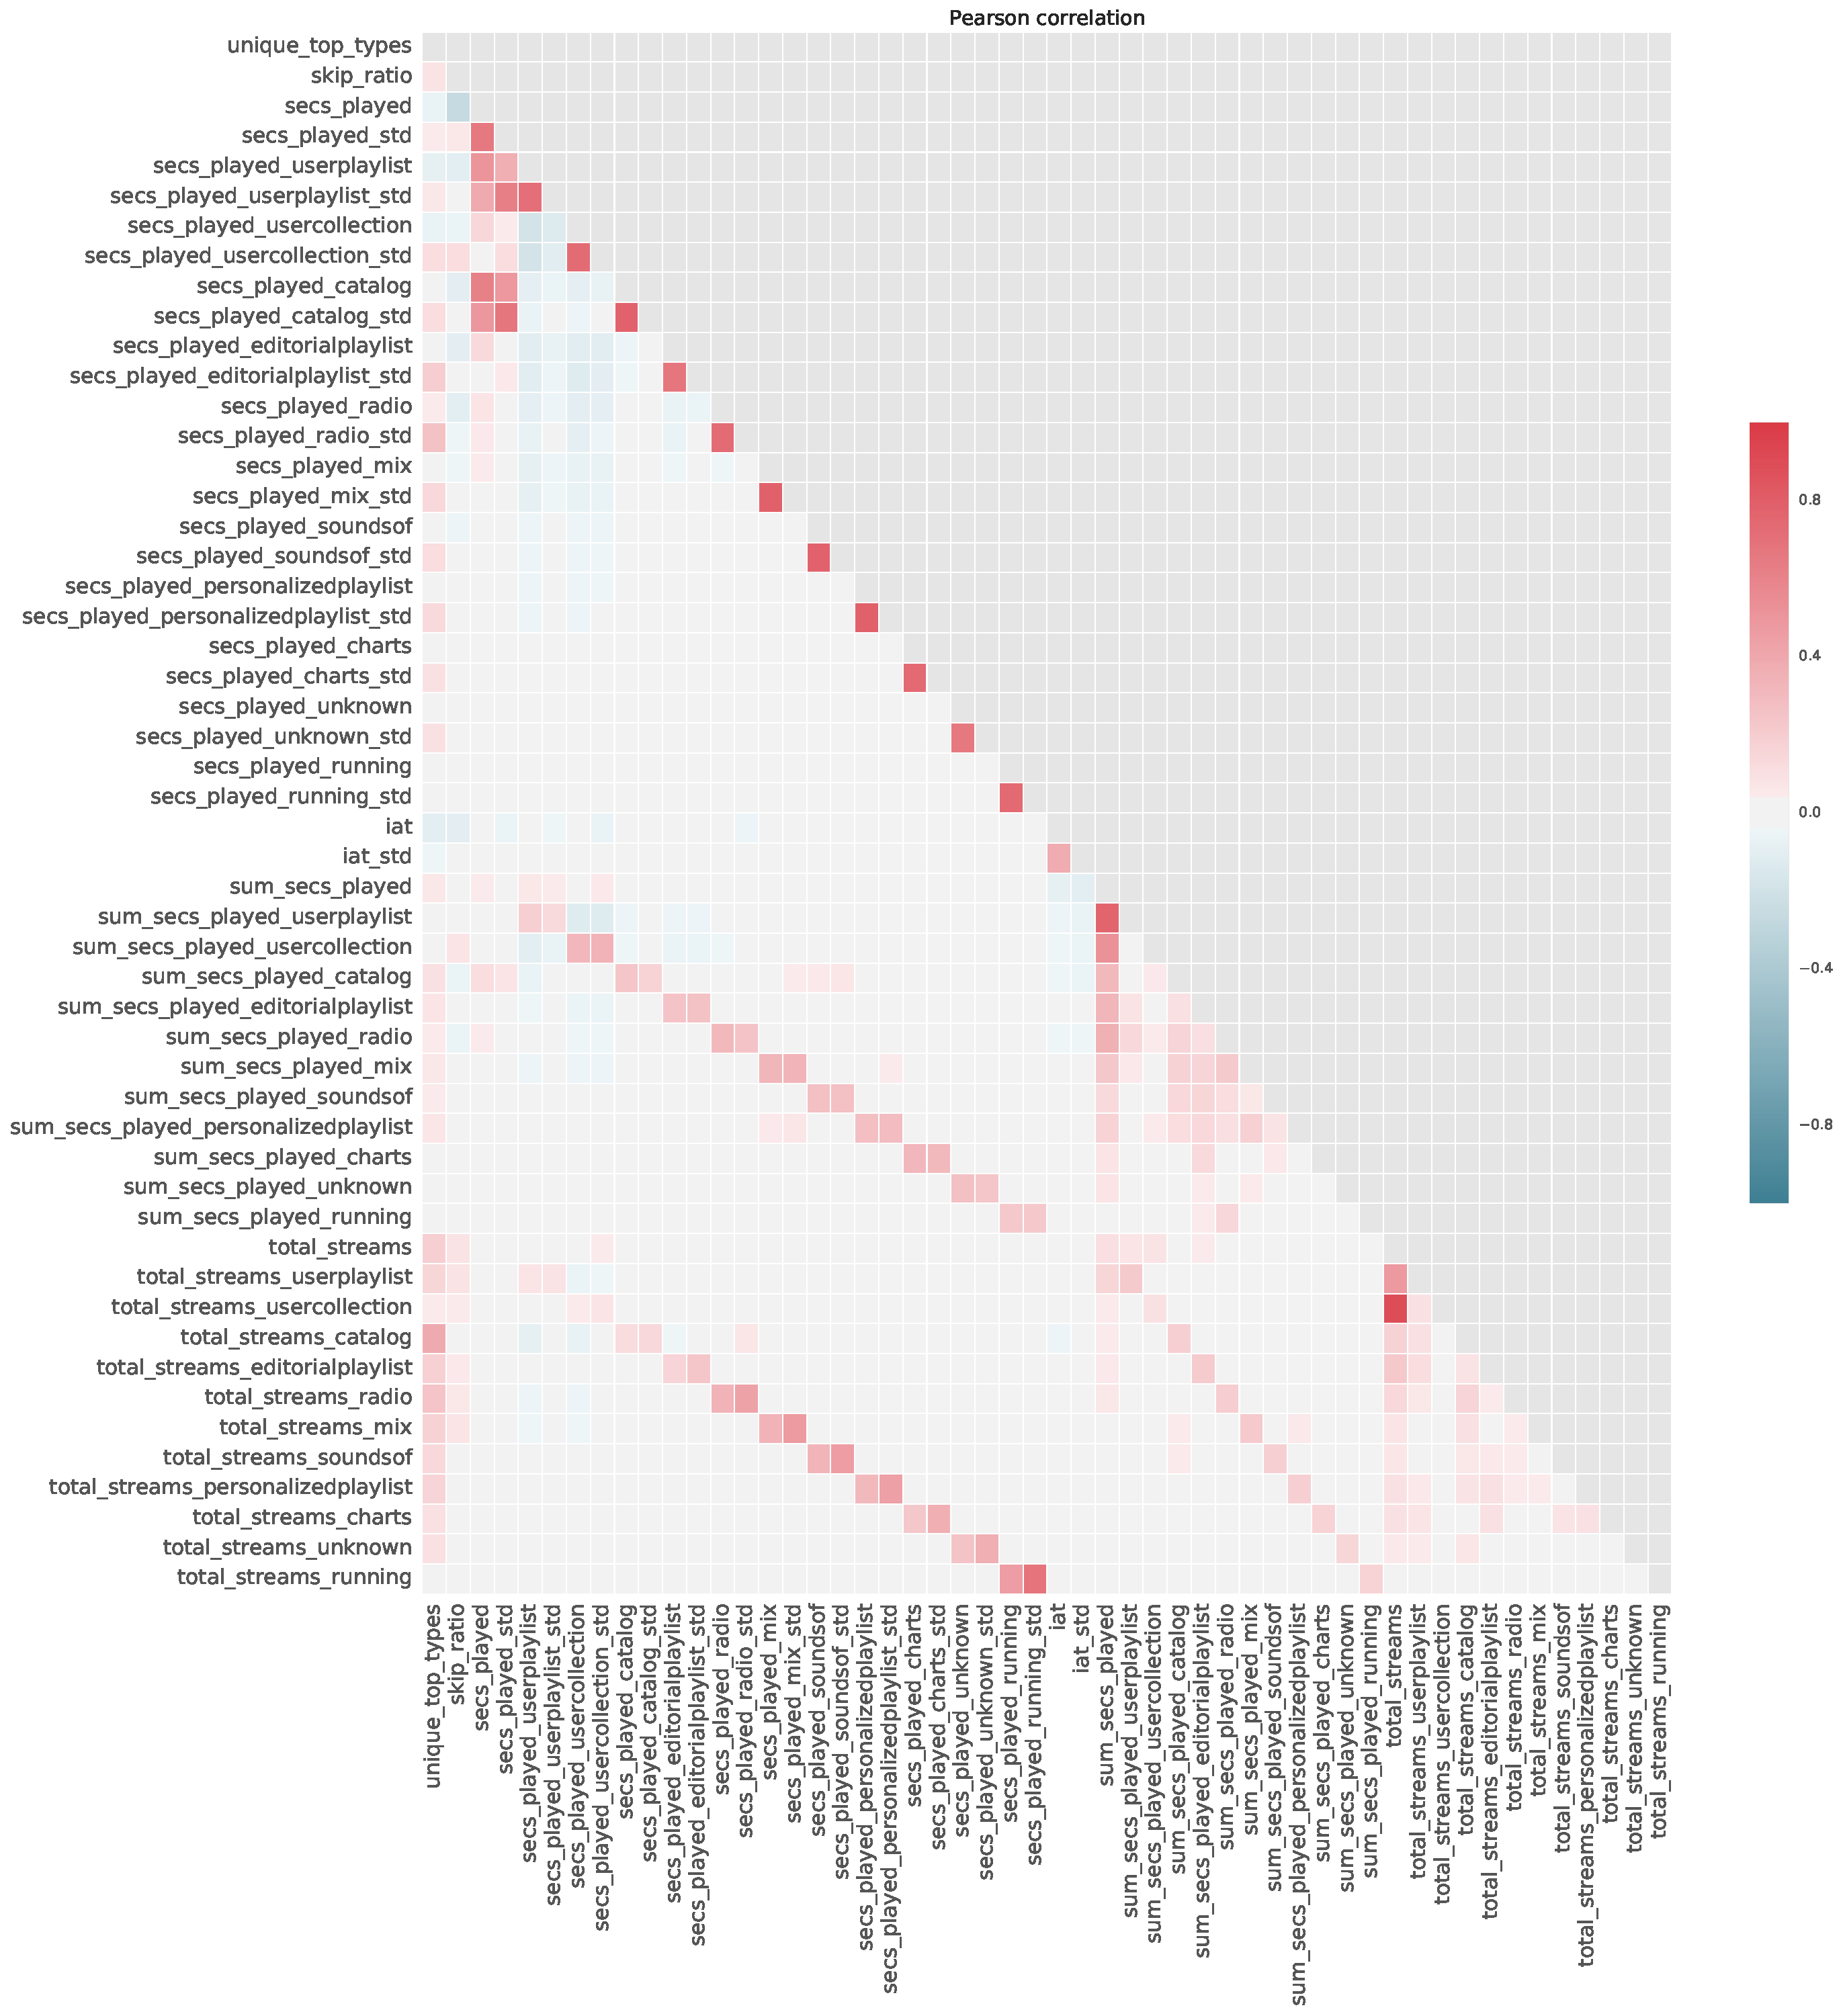
\includegraphics[width=0.9\textwidth,height=0.9\textheight,keepaspectratio]{figures/corr.pdf}
    \caption{Pearson correlation matrix between features}
    \label{fig:correlation}
\end{figure}

\subsection{Data Pre-processing}

The goal of the final stage of the pipeline is to transform the data into a format which is suitable to be used for training and that also improves convergence time of the learning algorithms. This is achieved by two main steps: normalization of the feature values and exporting the data into compressed files.

\subsubsection{Normalization}

While it is possible to use raw features as input to train predictive models, often there is a benefit on normalizing the values using some standard technique. \citep{lecun2012efficient} argues that for the backpropagation algorithm commonly used in neural networks, well-behaved features centered around and with unit variance usually provides a faster convergence time. This is mainly due to the way weights are updated in the network: if the input vector has all features with the same sign, the weights can only be increased or decreased together for a single input, zigzagging the values back and forth which turns to be extremely inefficient. In deep architectures, the output a network layer is used as input to the next layers, and for the same reasons it is also desirable that this input is centered around zero. Inputs with unit variance will keep the layer's output well behaved and thus speed up convergence.

Therefore, the following transformations were applied to the input before the training process:

 \begin{equation}
 \mu_i = \frac{1}{N}\sum_{n=1}^{N}x_n^i
 \end{equation}

\begin{equation}
\sigma_i^2 = \frac{1}{N}\sum_{n=1}^{N}(x_n^i - \mu_i)^2
\end{equation}
 
\begin{equation}
x_n^i = \frac{x_n^i - \mu_i}{\sigma_i^2}
\end{equation}

where $N$ is the total number of samples, $x_n^i$ is a scalar value representing the feature $i$ of the training sample $n$, feature which has mean $\mu_i$ and variance $\sigma^2_i$.

\subsubsection{Aggregating and Exporting}

After normalization, the feature values are in the desired format for training our predictive models, however they are still stored in an unsuitable location to be used as a source since all data is still stored as a table in BigQuery. Streaming the data directly from a cloud provider into the training algorithms, while is possible, depends heavily on the choice of programming language and the available distributed frameworks, and it also susceptible to engineering problems like the network connection between the cloud provider and the host where the models are going be trained on.

For this project, we decided to take a simpler approach and use compressed JSON line-delimited files as a data source for the training procedures. This format can be exported to through Google's web interface and also programatically through BigQuery's API, and be easily loaded using standard libraries in the most popular programming languages. The rows are processed and exported to files in parallel, greatly accelerating the procedure.

We need to take some precautions for the export process to work flawlessly, however. The source table containing all the training data is stored in a long format, that is one row per user per time step. Since the export procedure is performed in parallel, the entries for a single user might end up spread into different files. To avoid having to fix this in the training functions, we apply a simple aggregation to group all time steps belonging to a user into a single row.

\section{Data Exploration}

"Get to know your data" is a common jargon in the data science field, and for a good reason: even the smartest learning algorithms may fail to perform well if the data used as source is of questionable quality. Understanding how the data is distributed is of utmost importance, not only to gather insightful information that may be used in our advantage for training our predictive models, but also to validate that our dataset creation algorithm is free of mistakes and is representative of the target audience. This section will be dedicated to visualizing the data created through the pipeline described in the previous sections.

The large amount of rows in the dataset makes it difficult to plot it using standard well-known visualization libraries. Therefore, a sample of 1\% of users was selected for the following plots, totaling 5125 unique users and 861000 rows of data corresponding to the 56 days of observation time.

Due to privacy concerns and the signed non-disclosure agreement between the interested parties in this project, some of the tick labels in the graphs were intentionally left out.

\subsection{User Distribution}

A recurring problem in churn prediction is how the non-churning class dominates over the churners for almost all applications, a problem properly examined by \citep{Burez2009}. \Cref{fig:classdist} plots the distribution of classes in our generated dataset. In it we can observe that the churning class is the overwhelming minority of our samples. This heavily imbalanced dataset may pose several challenges when training our models, since learning algorithms may fail to capture the nuances of user churning behavior with a lack of representative samples.

	\begin{figure}[H]
    \centering
    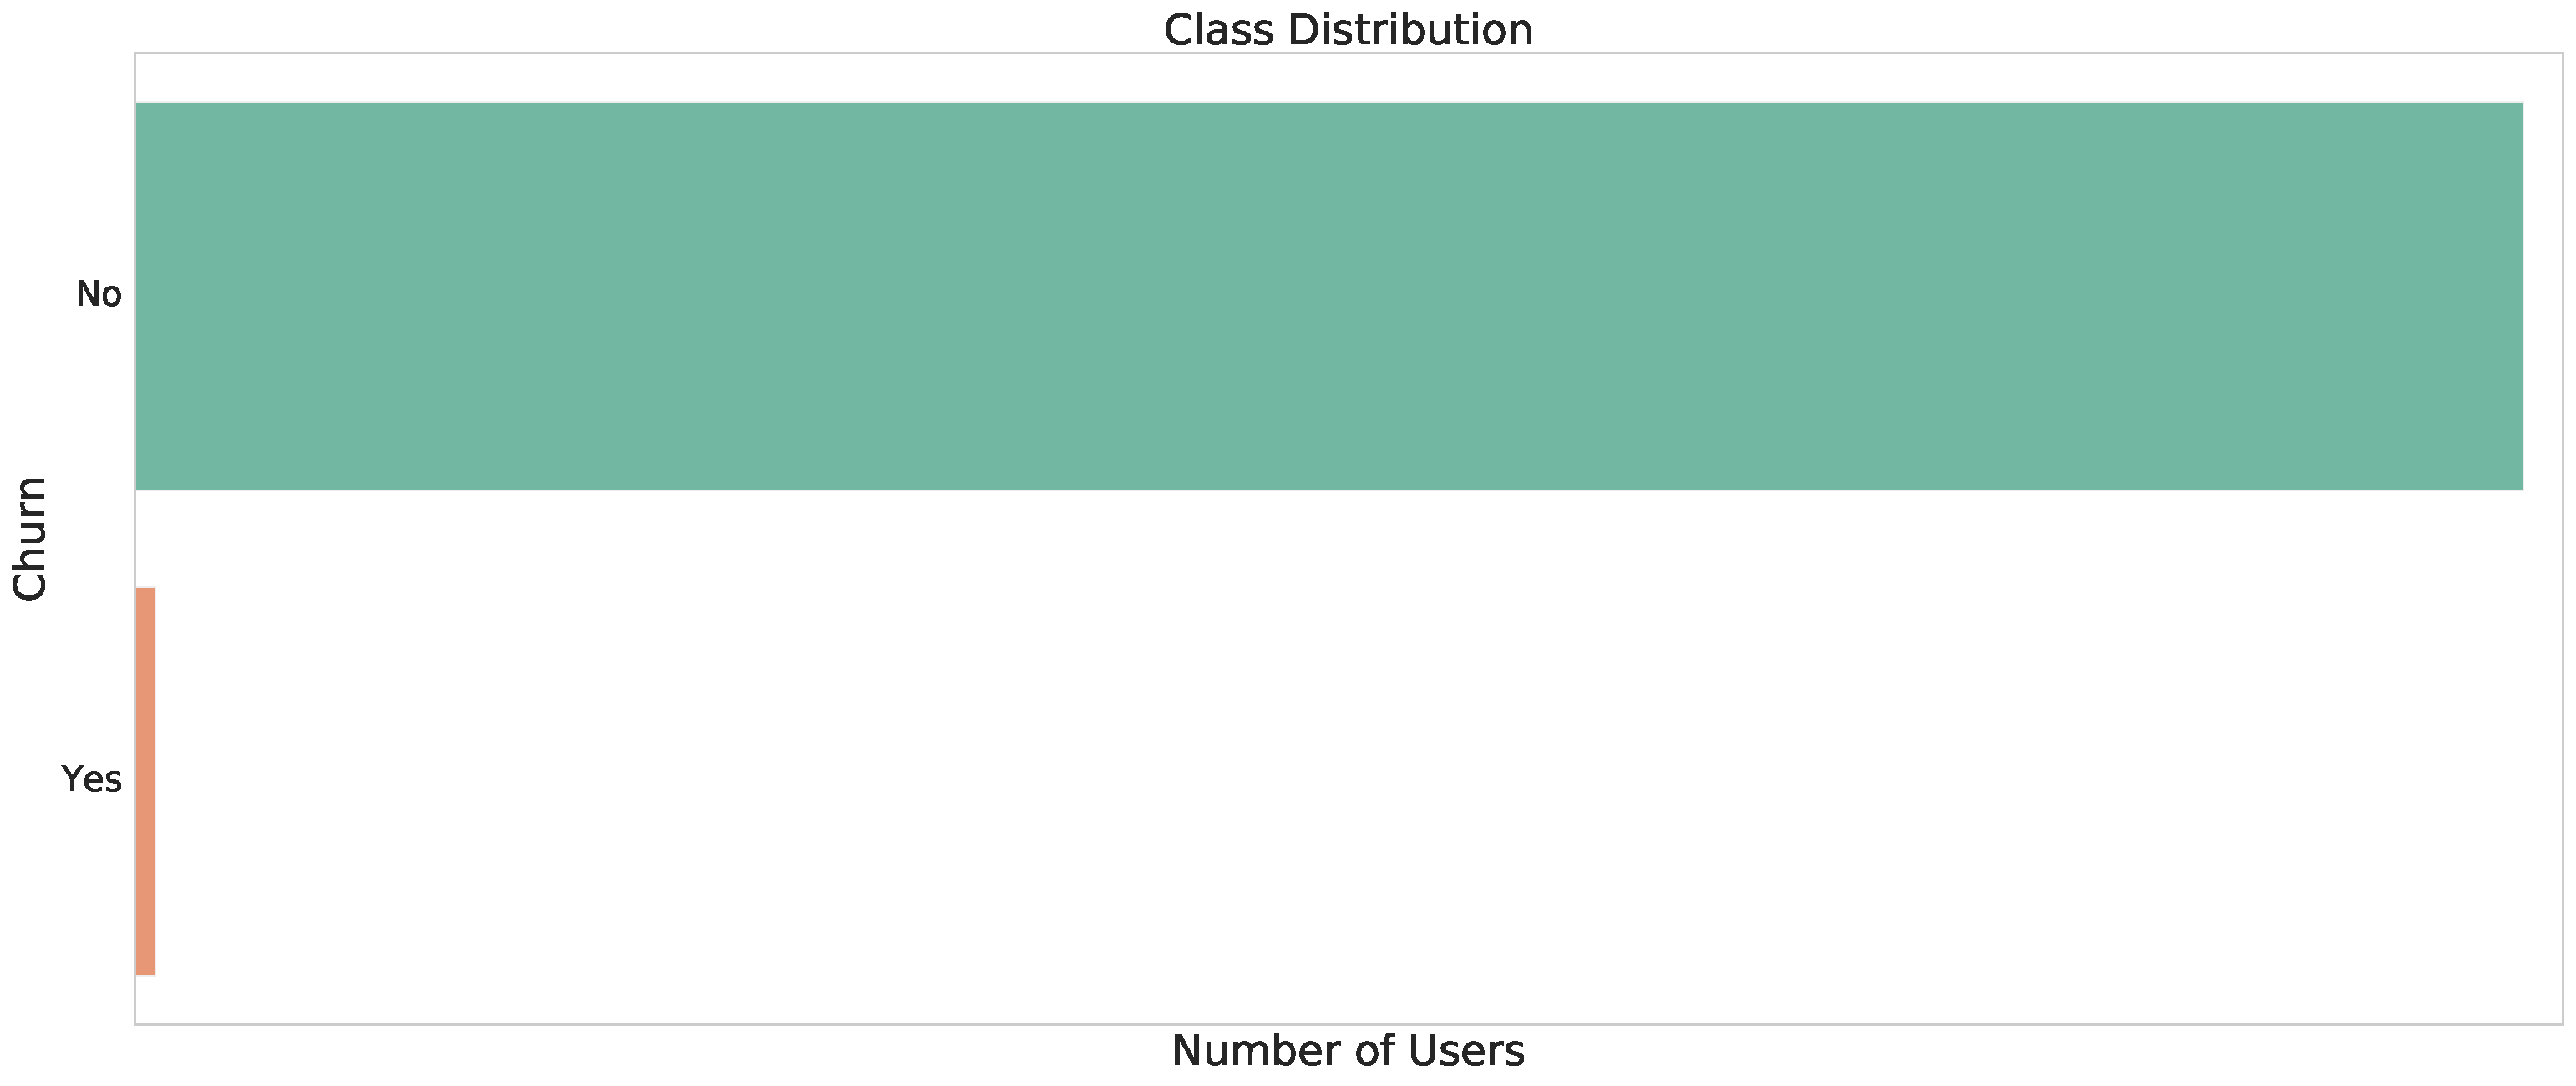
\includegraphics[width=0.9\textwidth,height=0.9\textheight,keepaspectratio]{figures/class_dist.pdf}
    \caption{Count of users distributed in the churn and non-churn classes}
    \label{fig:classdist}
	\end{figure}

Streaming products are either in paid-subscription form available to the users or in a free version with some limitations such as restricted catalog or streaming advertisements between content. The data exploration indicated that, as expected in our case-study, users with paid-subscriptions are retaining better. This translates to seeing more churned users in free user cohort. This behavior is understandable due in parts to how easy it is to abandon the service without a formal contract attached, and also by the restricted experience that free users are exposed to when compared to paid-subscription version of the service.

The initial data exploration showed that the ratio of churn over retained users varies in different countries. We therefore decided not to limit the user samples from one country but to collect instead the data from major markets that are representative of most of the users utilizing the product.

Users show different behaviors whether they registered for a long time or if they just created their accounts. Internal studies showed that long-term users reveal a more stable behavior on application usage when comparing to recent arrivals. Also, activating new users into the platform is a challenge in itself, until the customer learns how to use the product, identifies the features that likes more or is more comfortable with it. \Cref{fig:dayssinceregdist} plots the number of days since registration between the churning and retained classes, it can be visualized how churning users are concentrated on the range of new users, while the retaining class is more uniformly distributed along the x-axis.

	\begin{figure}[h]
    \centering
    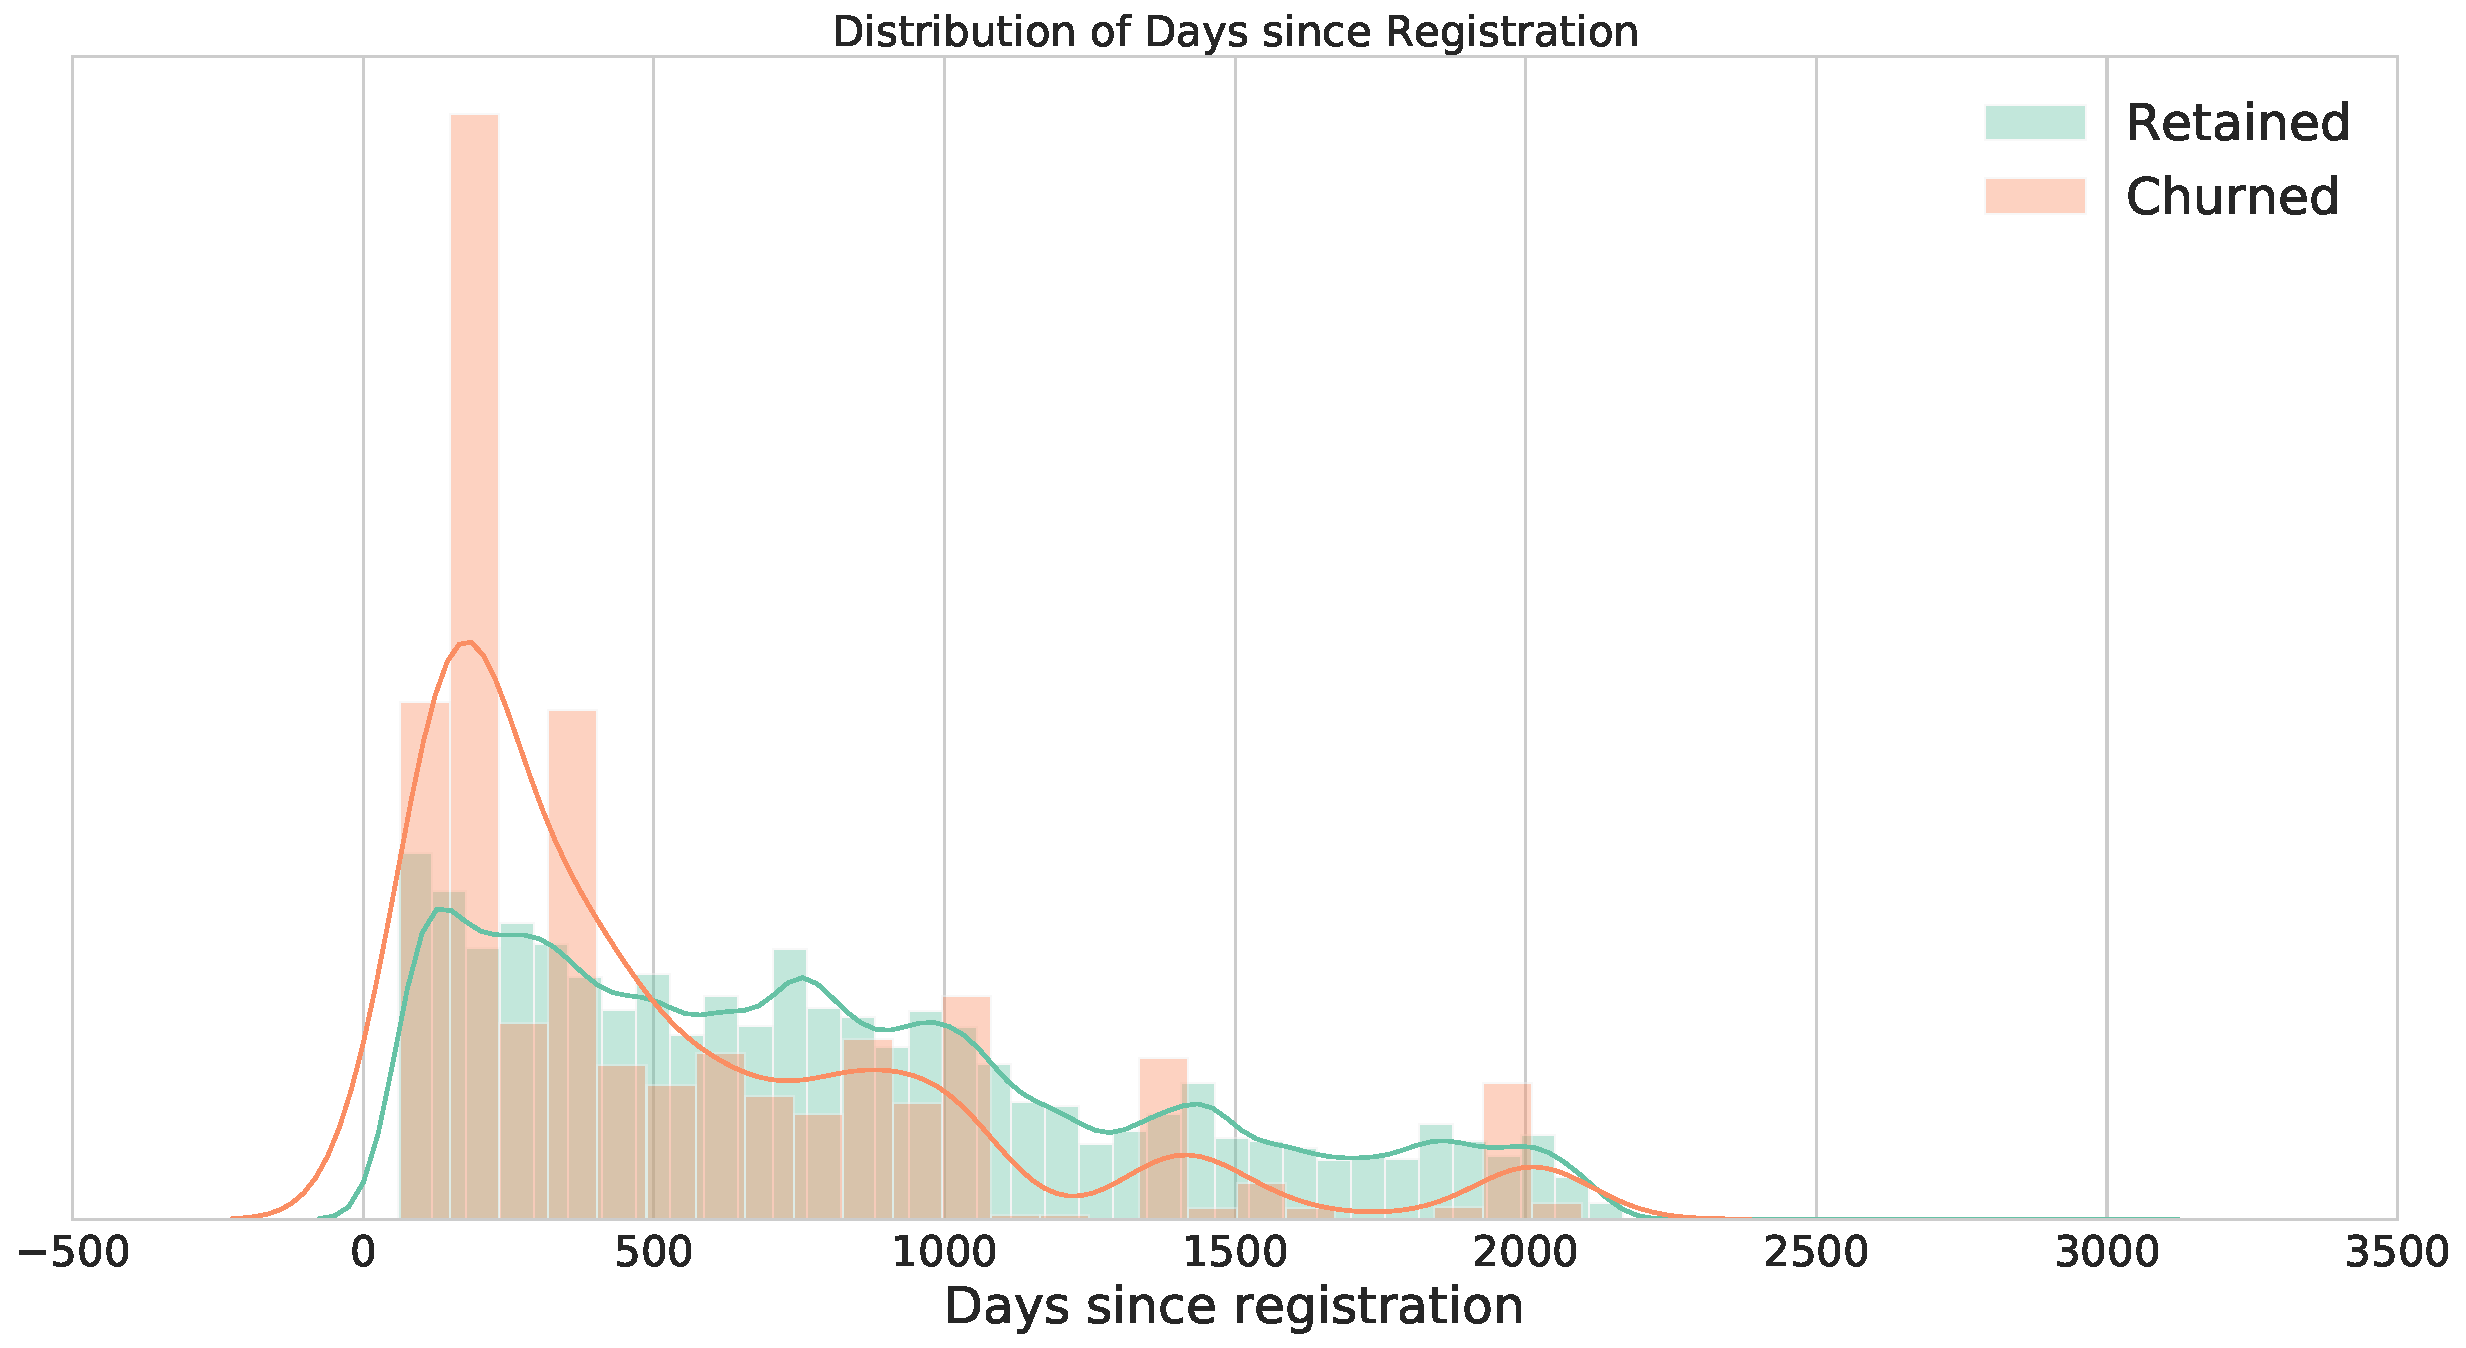
\includegraphics[width=1.0\textwidth,keepaspectratio]{figures/days_since_reg.pdf}
    \caption{Users distribution over days since registration and churn label}
    \label{fig:dayssinceregdist}
	\end{figure}

\subsection{User Behavior Through Time}

Humans are creatures of habits. Our daily routines follow distinguishable patterns mainly influenced by day-night cycles that are far from being random. To better visualize these patterns, \Cref{fig:featstime} plots the feature values for churning and retaining users over the course of the observation window sized at 56 days. 

The first pattern that can be noticed is that users that are labeled as churning have lower values for features when compared to those who are retained in the service. This difference can be perceived in the consumption time (the average number of seconds in all streams in the time step), total streams (the count of streams in each time step) and sum consumption time (the accumulating sum of seconds played in streams) features. These are all features that indicate usage: users that interact with the application more often and for more time are more likely to be retained.

The second trait that can be observed is that skip ratio has a smaller gap between the churning and retaining classes when compared to other features. A previous study from the service provider suggests that users who churn have higher skip ratio values, however this is counter-balanced by the fact that absent users cannot skip since no content is being streamed.
	
	\begin{figure}[h]
    \centering
    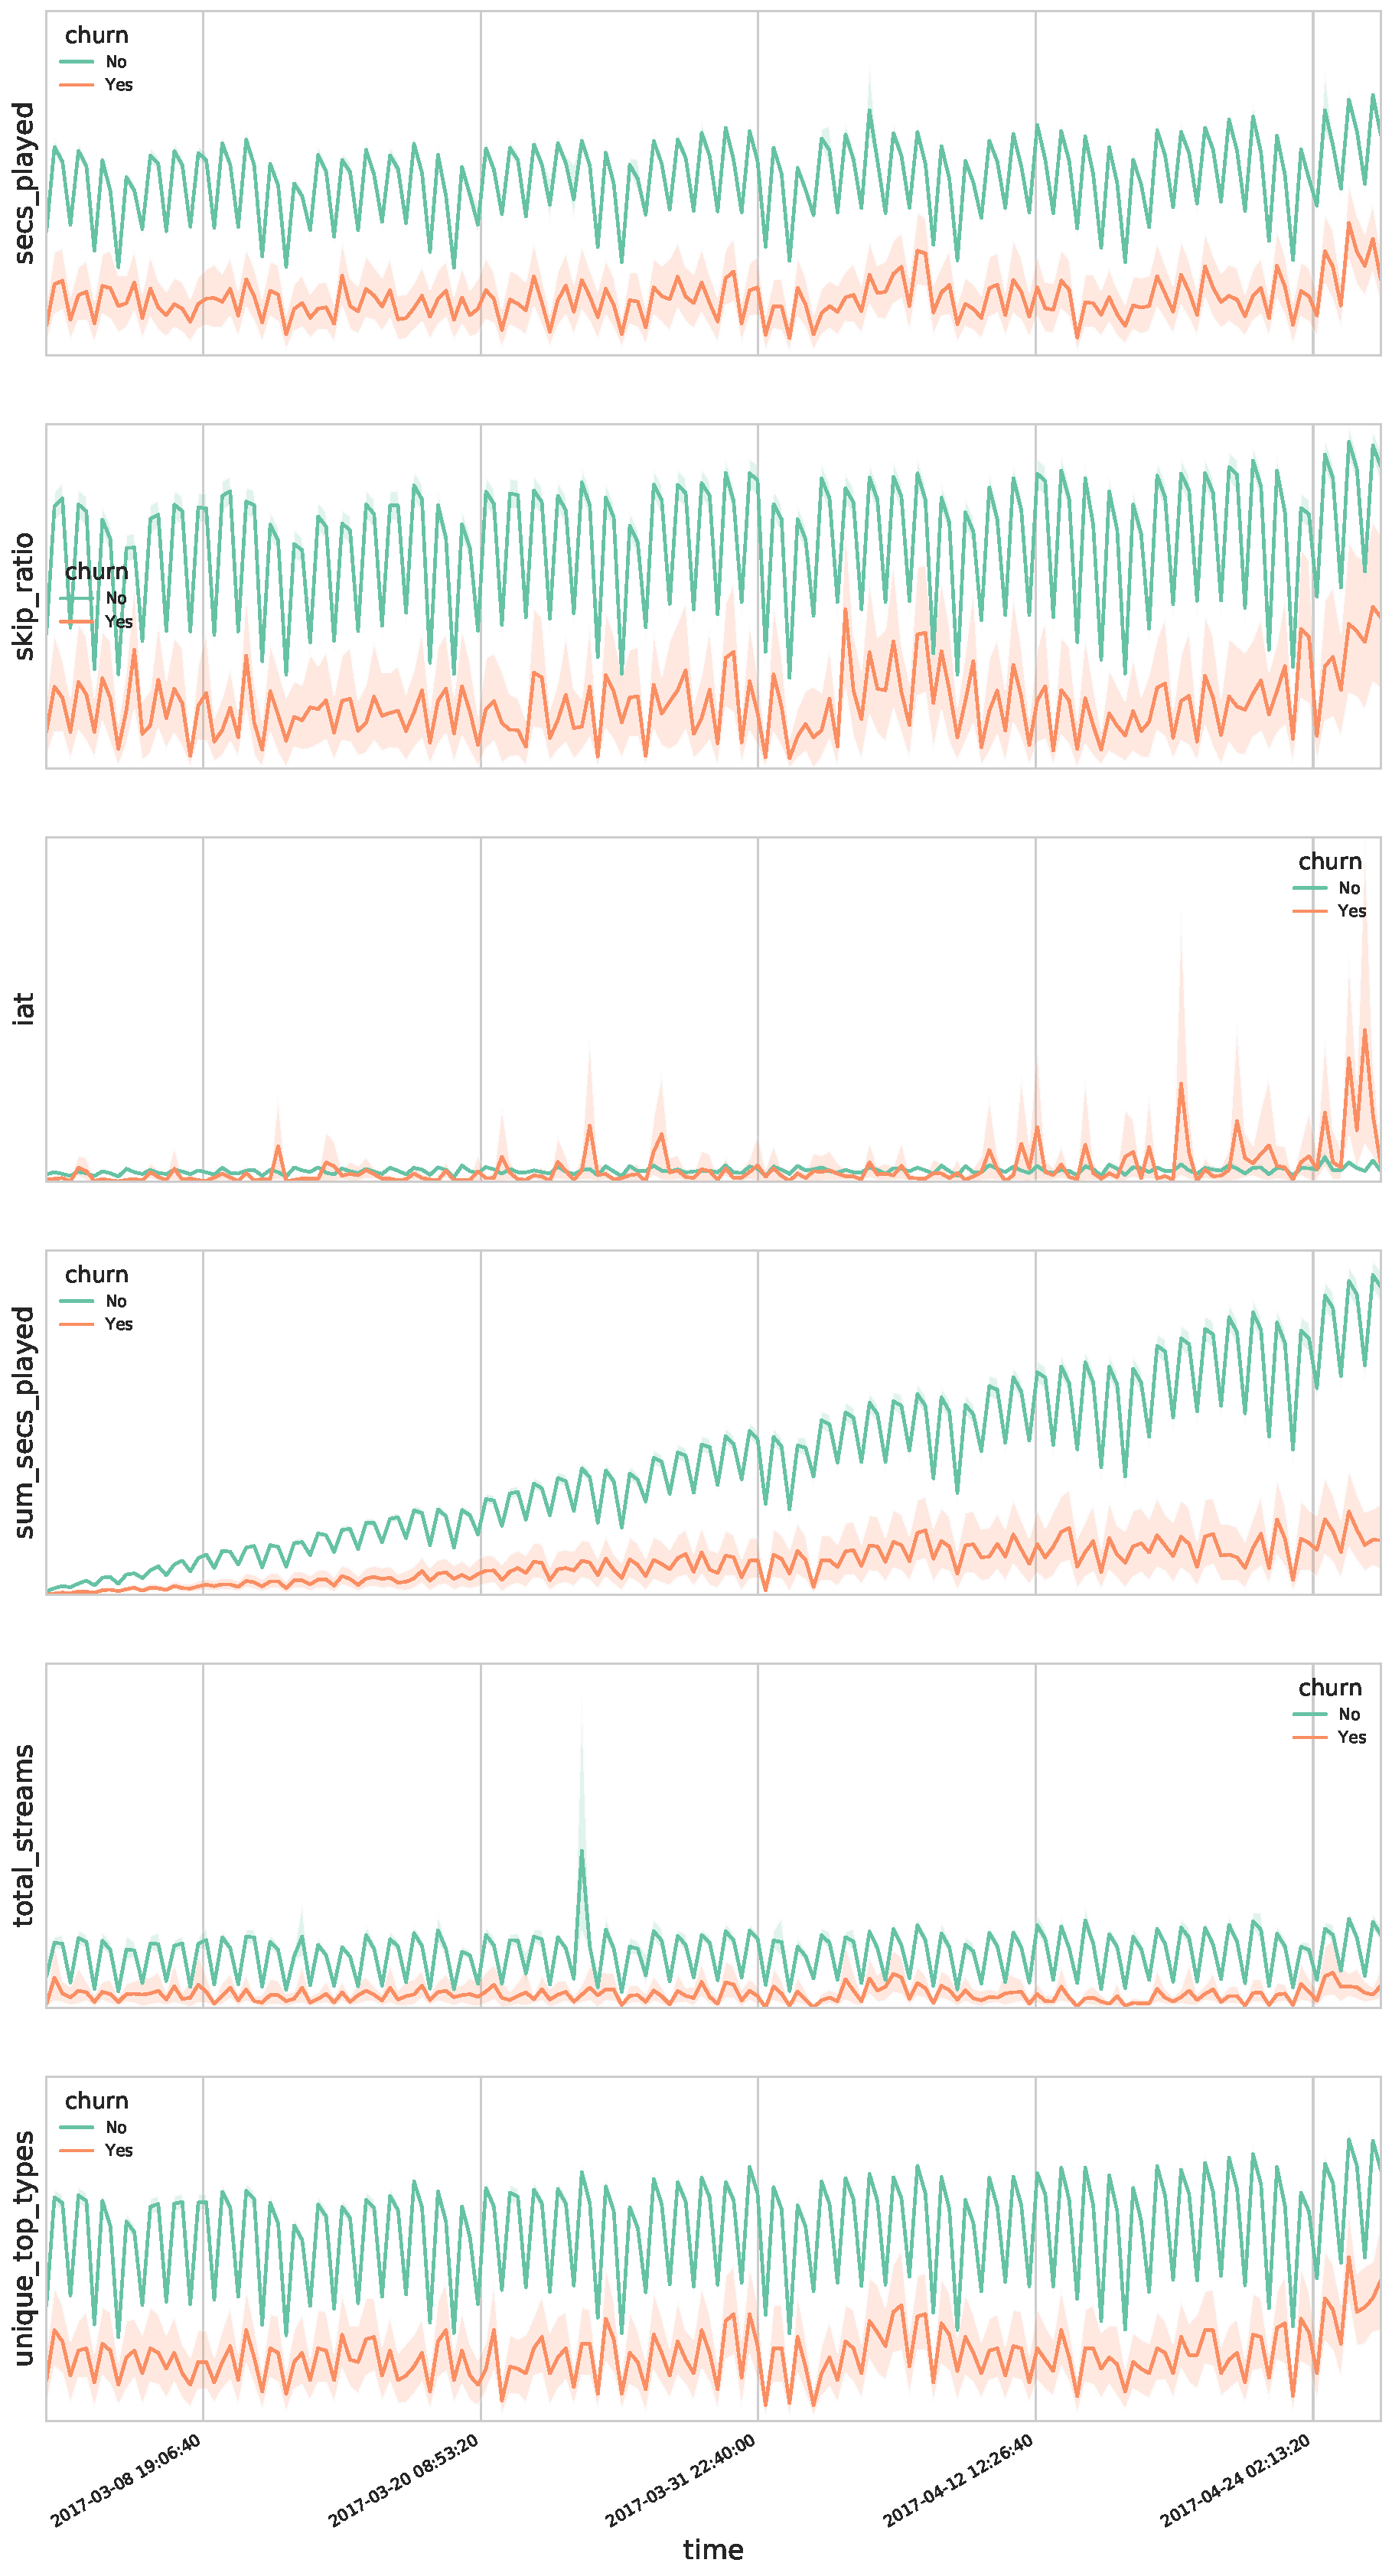
\includegraphics[width=1.0\textwidth,height=1.0\textheight,keepaspectratio]{figures/feats_time.pdf}
    \caption{Mean values of features throughout the observation window}
    \label{fig:featstime}
	\end{figure}

\subsection{Feature Correlation to Churn}

One question that can be answered is how does any of the generated features correlates to the churn label. Do they exhibit a positive or negative association? Even though it is known that correlation does not necessarily implies a causal relationship, it may still be interesting to observe what is the overall tendency of the features when they are associated with churn. To accomplish this, a \emph{point biserial correlation coefficient} is the correct tool to use when one of the variable is continuous and the other dichotomous, and its plot can be seen in \Cref{fig:corr_pbs}.

Some interesting relationships can be observed. First, the plot shows that IAT features (inter-arrival time between streams) are the ones with the strongest association to the positive churning label, which is understandable: users that do not come back to the application as often are not making use of the service at its fullest and are more likely to abandon it. Second, the sum consumption time group of features are in its majority negatively correlated with churn, which strengthens our hypothesis that customers who use the service more often are less likely to abandon it. 

Looking at different content consumption features, we observed a non neutral (positive or negative) correlation with user churn. Further studies in future on this can shed light on how and when to provide content to user.

Lastly, a rather surprising result is that the number of unique contexts have a positive association with churn. Our hypothesis is that users who are new in the platform posses a more explorative behavior by trying several different features when compared to users who are in the platform for a long time. As could be seen in \Cref{fig:dayssinceregdist}, churning users are commonly newer in the service when compared to retained ones. 

	\begin{figure}[H]
    \centering
    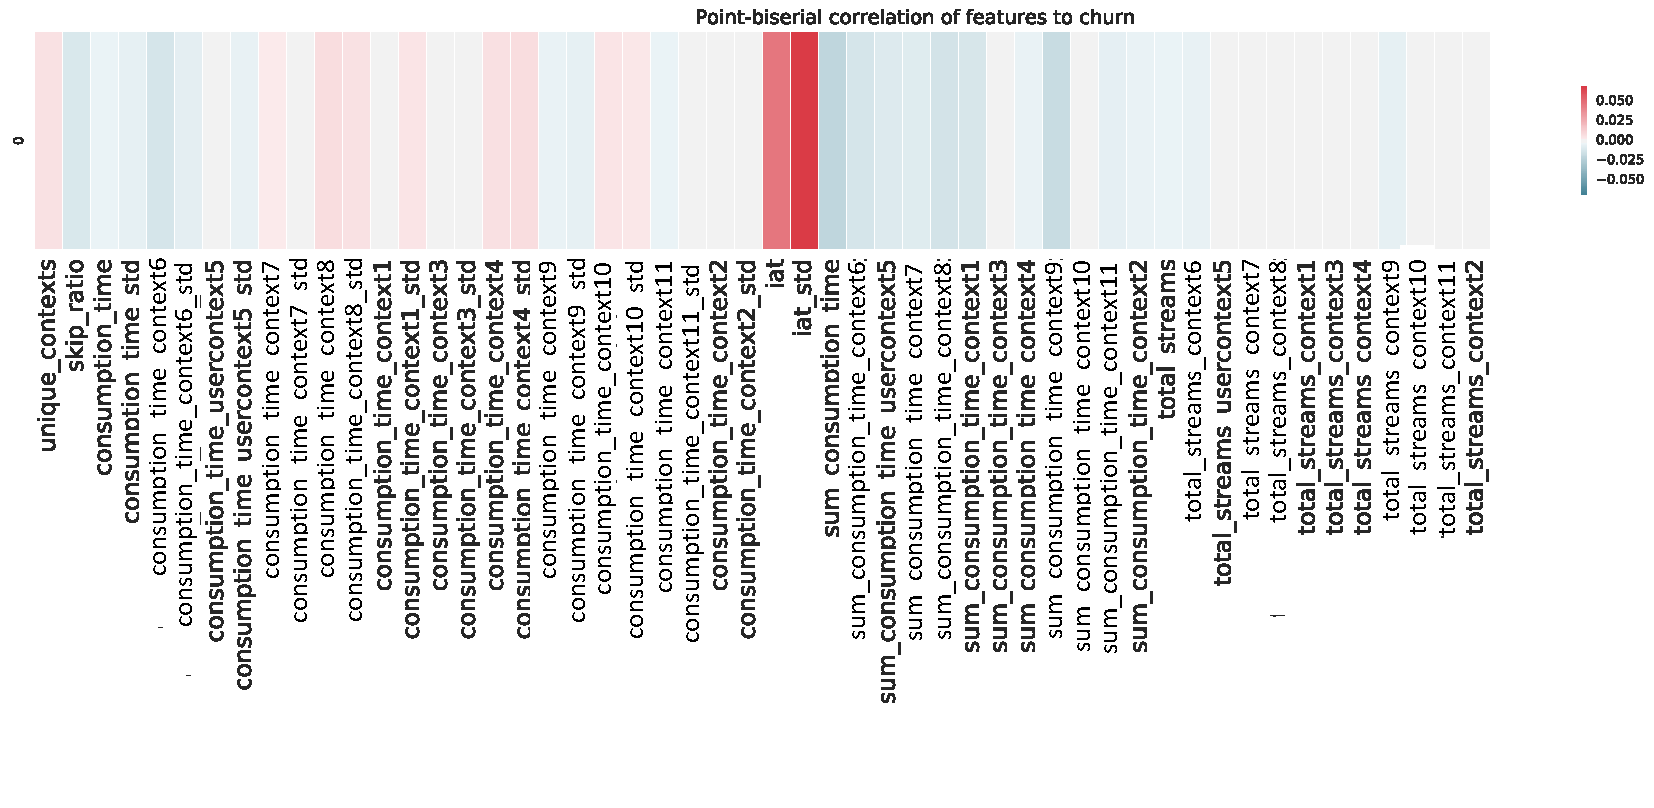
\includegraphics[width=0.9\textwidth,keepaspectratio]{figures/corr_pbs.pdf}
    \caption{Point-biserial correlation between features and the churn label}
    \label{fig:corr_pbs}
	\end{figure}

\subsection{Dimensionality Reduction}

Although the features generated through our data pipeline encompasses different aspects of the users behavior in the platform, it may pose a challenge regarding the high dimensionality of our dataset: machine learning models may have trouble extracting the latent information from feature values if data is not sufficient. Since our dataset is heavily imbalanced, the number of available samples for the churning class may be insufficient, and using a more compact representation of the data may prove fruitful when the goal is to maximize the score of our predictive models.

Principal Component Analysis (PCA) is popular technique that strives to find a lower dimension representation by keeping most of the variability of the data, or as described by Hotelling \citep{hotelling1933analysis}, it is, for a given set of data vectors, the $d$ orthonormal axes onto which the variance retained under projection is maximal.

In \Cref{fig:pca_data} we can visualize the data distribution when its dimensionality is reduced to its two principal components through PCA for both retained and churned classes. It can be seen that the distribution between classes overlap in the projected plane, however their center points are clearly apart from each other.

	\begin{figure}[h]
    \centering
    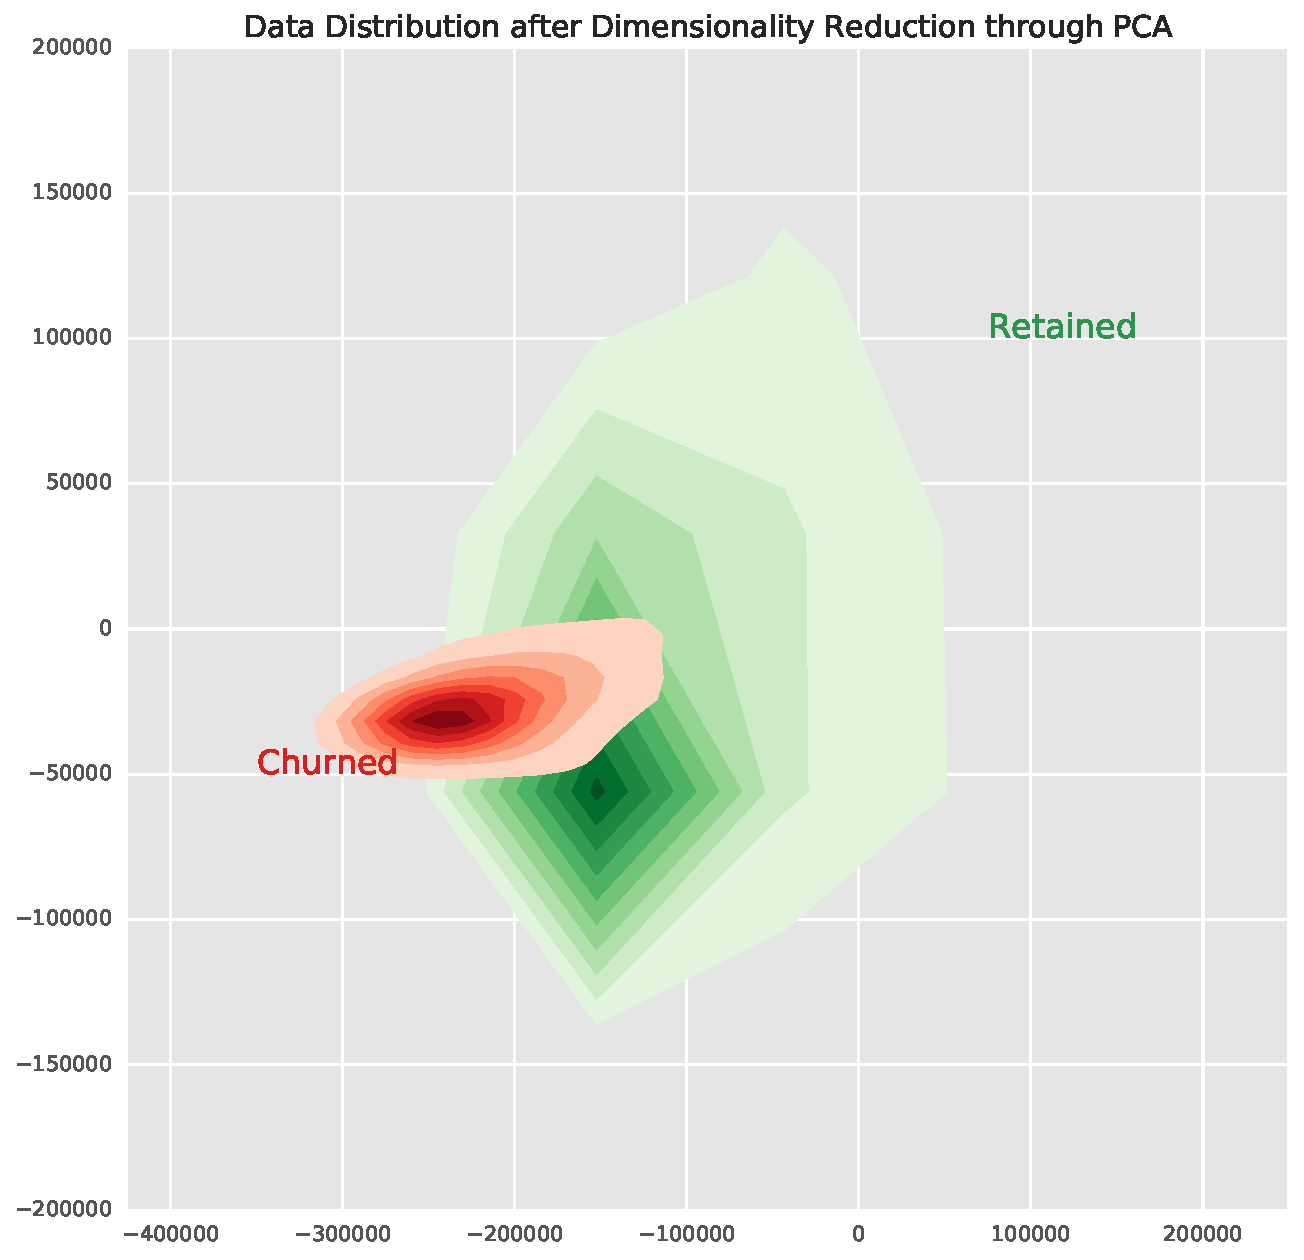
\includegraphics[width=0.9\textwidth,keepaspectratio]{figures/pca_data.pdf}
    \caption{Data distribution after reducing to 2 principal components through PCA}
    \label{fig:pca_data}
	\end{figure}

\section{Software and Libraries}

Manipulating large quantities of data is a task that cannot be performed easily using standard libraries of a programming language. The pipeline creation was only made possible in the scope of this project by making use of frameworks for massive data manipulation available for this master thesis work.

The sampling, extraction and pre-processing steps of the data pipeline were performed using Big Query \citep{sato2012inside}, a fully-managed and cloud-based interactive query service for massive datasets created by Google. The parsing and pre-processing step was partially performed in Scio \citep{scio}, a Scala API for Apache Beam and Google Cloud Dataflow.

\chapter{Methodology}
\label{cha:method}

Creating experiments that are reliable, reproducible and as unbiased as realistically possible is a challenge for any researcher interested in obtaining results that can safely be reasoned on. It is made harder by the complexity of our own source dataset: human behavior is far from being a process easily predictable due to the sheer amount of latent variables that may influence the outcome of the experimentation process.

This chapter is dedicated to present to the reader a detailed picture how the experiments were performed, the choices of classifiers, the way they were optimized to the best set of parameters, and how the final score for each model was obtained.

\section{Handling the Class Imbalance Problem}

For any relatively successful company the non-churning class heavily outweigh the amount of churners in the dataset. Depending on the estimator, this property can have a negative impact in performance where the models only can only learn how to distinguish the majority class and failing to detect the class of interest. However empirical observations have shown that a better performance can be achieved if the class ratio difference is reduced  \citep{Burez2009} \citep{ling1998data}. 

There are three commonly used sampling techniques for dealing with heavily skewed datasets: 

\begin{itemize}
\item Undersampling by removing samples from the majority class using a pre-defined selection technique
\item Oversampling by creating artificial samples that closely mimics the true data present in the minority class
\item A combination of over and undersampling, commonly oversampling the minority class first and reducing the data in the majority class second.
\end{itemize}

Unless otherwise stated, the experiments in this project will be \emph{randomly undersampled} to a class ratio of 1-to-1. This technique, while easy to implement, throws away several samples from the majority class that could be used for learning. Testing different ratios for the class distribution is however one of the experiments that will be performed in this project. 

\section{Cross-Validation}

It is a common  practice in supervised machine learning experiments to split the data sets into \emph{train} and \emph{test sets} as to obtain an unbiased estimate of the performance of the trained models on unseen data: evaluating a model on the data it was trained on can return an overly optimistic score that does not generalize well for data that is not included in the training, a phenomenon called \emph{overfitting}. Therefore, every score in this project is reported using data that was not present in the training stage.

Almost all machine learning predictive models have arguments that needs to be chosen even before the training process starts, values that are commonly called \emph{hyperparameters}. To fine tune these parameters, we need a method to evaluate how good a set of values are against all other (or a reasonably sized subset of) available options, and for that purpose we need a set of unseen data for the same reasons mentioned before. If the test set were used for such an evaluation, it could not be considered as unseen data anymore since it was used for the purpose of choosing the best model, thus our bias may have "leaked" to the prediction score. Therefore another set is needed to tune the hyperparameters, which is commonly called the \emph{validation set} in the machine learning domain.

Dividing the dataset into three splits however drastically reduces the number of samples that ares available for model learning. Another concern is that if the sets are unique, the overall performance metric will depend in a seemingly random split of validation and test sets. To mitigate this problem, a technique called \emph{cross-validation} can be applied\citep{stone1974cross}. In its most basic approach, instead of having a single validation set, the training set is instead divided into $k$ folds, and at each hyperparameter tuning round the model is trained on $k-1$ folds and validated on the fold that was left out. For each set of parameters, $k$ models are generated, and the final metric can then be an aggregation function over all estimators performance, like the mean. After selecting the best set of parameters, another training session can be made with the union of the data available in all folds, thus acquiring a tuned version of the model.

The above technique helps to strengthen our performance metric against biases when selecting the best set of hyperparameters to train our model with. However we still have an unique test set where we evaluate our model to obtain a final score. When comparing different types of estimators, it may happen that one estimator may better learn from the samples that are on the training set while the other can better learn from the patterns contained on the samples of the test set, a split that was purely made by chance. This may lead to a form of selection bias resulting in overly-optmistic scores \citep{cawley2010over}. The same procedure used for hyperparameter tuning can be applied for splitting the train and test sets, a technique called \emph{nested cross-validation}. In it, the full dataset is split into $k$ outer folds of training and test sets, and each training set is further split into $l$ inner folds for hyperameter tuning.  A diagram of this procedure can be seen in Figure \ref{fig:crossval}.

	\begin{figure}[h]
    \centering
    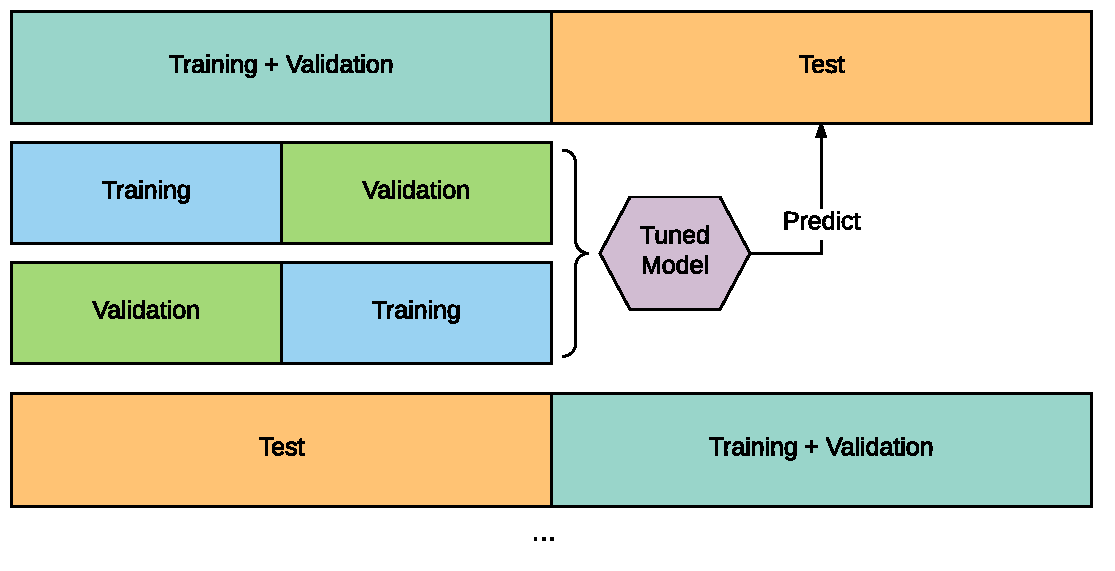
\includegraphics[width=0.8\textwidth,keepaspectratio]{figures/crossval.pdf}
    \caption{2x2 nested cross validation}
    \label{fig:crossval}
	\end{figure}

Even though this technique increases the confidence of our metric scores, there is a price to pay in terms of performance: training all these models may take a considerable amount of time. The service provider however has no lack of computational resources available, so this project makes use of this method. Inspired by \citep{Burez2009}, all our models were trained using \emph{2$\times$2 cross-validation}, with 2 outer folds for the train/test split and 2 inner folds for train/validation splits.

\section{Hyperparameter Search}

Lastly, a proper method needs to chosen to perform search over the domain of parameter values. A common practice in machine learning model training is to perform a parameter sweep by exhaustively searching a subset of values manually chosen by the experimenter. This method is called \emph{grid search}, and due to its simplicity and reproducibility is one of the most used techniques, be it for classical machine learning algorithms like Support Vector Machines as to deep feed-forward neural networks \citep{larochelle2007empirical}.

However, performing a grid search over every combination of values can quickly turn it into a method which is too computationally expensive to perform for any real-world applications. Deep architectures like LSTMs are known to be costly to train, and combining it a full parameter sweep is prohibitive if the dataset in question is of a respectable size. Bengio and Bergstra\citep{bergstra2012random} have demonstrated that, for neural networks, performing a \emph{random search} over the same parameters domain can result in a model which is as good or better than the one validated through grid search by using a fraction of the computation time. 

In a random search, parameter values are randomly sampled from a specified distribution instead of being chosen directly from a grid. For a set number of rounds, samples are gathered for every parameter and used for model validation. This allows us to set a processing budget which is independent of the number of parameters available and the number of possible values for each. Therefore, adding parameters that have no impact in performance will not decrease the efficiency of the cross-validation process for no gain. 

The experiments performed in this project make use of both methods: for the classical Logistic Regression and Random Forests, a grid search over a pre-selected set of values was the chosen method, since their training time is commonly faster when compared to regularly sized deep neural network. Random search is the technique used for validating parameters of our LSTM models, since it is too expensive to compute with a parameter sweep due to its long training time. The set of parameters used for the experiments follows:

\begin{itemize}
\item Logistic Regression
\begin{itemize}
\item C (inverse of regularization strength): 0.01, 0.1, 1, 10, 100
\item Regularization method: L1-norm, L2-norm
\end{itemize}
\item Random Forest
\begin{itemize}
\item Number of estimators: 10, 100, 500, 1000
\end{itemize}
\item LSTM
\begin{itemize}
\item Number of layers: 1 to 3
\item Units per layer: 64 to 256
\item Optimizer: RMSprop, Adagrad
\end{itemize}
\end{itemize}

\section{Model Training}

Even though all models were trained with the same source dataset, temporal and time-invariant models requires a different representation of the data, a topic which was explored in \Cref{sec:timewindows}. Logistic regression and random forest models were both trained with the SPTD version of the dataset using the mean as the aggregation function $f$, while the LSTM models were trained with the full unrolled MPTD data.

When analyzing the data contained in the MPTD dataset, a property that could be observed is that the feature values are sparse. This is due to the representation chosen for the absent user in a specific time step: users that did not stream any song during an 8 hours interval will have its features all set to zero. We can leverage this property through a data structure that better utilizes memory resources by storing only the non-zero entries instead, which is accomplished by representing the data with a \emph{compressed sparse row} structure \citep{bulucc2009parallel}. This allows us to store the data in memory in a single machine without resorting to distributed algorithms which would make the implementation more difficult.

To increase the reproducibility of our experimentation process, the same seed value was used for all random factors contained in the experiments. That includes the dataset fold splitting, random search, weights initialization in LSTMs and the undersampling. The seed value chosen was 42, which is the answer to the ultimate question of life, universe and everything \citep{adams1995hitchhikers}.

\subsection{The LSTM Recurrent Network}

This section describes some details about the LSTM models used in the experiments of this project.

Since the number of layers is a parameter that is being tuned during the cross-validation phase, the exact architecture of the LSTM varies depending on the training and validation data. It is beneficial however to visualize the overall structure of one choice of model parameters as to better understand how the layers are organized, which can be seen in \Cref{fig:lstm_arch}.

	\begin{figure}[h]
    \centering
    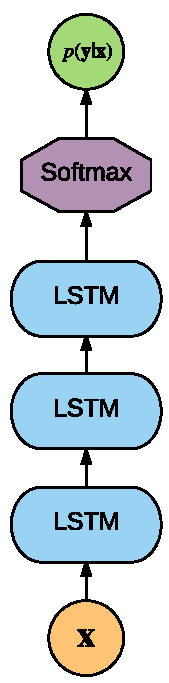
\includegraphics[height=0.7\textwidth,keepaspectratio]{figures/lstm_arch.pdf}
    \caption{Model architecture with 3 stacked LSTM layers}
    \label{fig:lstm_arch}
	\end{figure}

In this example, three LSTM layers were stacked on after the other, each one with a different number of units per layer chosen through random search. A softmax layer transforms the output of the last LSTM layer and transform it into a probability distribution over the two retained and churned classes.

Every model was trained for 100 epochs using a batch size of 512, a number chosen for performance reasons. The optimizers were initialized with a learning rate of 0.001. For Adagrad, the value for the fuzz factor $\epsilon=1\times10^{-8}$ applies. RMSProp also has the same $\epsilon$, adding $\gamma=0.9$ which regulates how much of the previous average of gradients shall be used to calculate the current gradients .

The weight matrices for the linear transformations of the input were initialized with Xavier initialization method, while the ones corresponding to the linear transformation of the recurrent state were initialized with a random orthogonal matrix. Bias vectors were initialized to zeros since the asymmetry breaking is already performed by the chosen weight initialization algorithm.

The loss function is binary cross entropy. All parameters were regularized with $L_2$ weight decay method, using a regularizing factor of $0.01$.

\subsection{Training Procedure}

We summarize the training process in Algorithm \Cref{alg:train}. This procedure is applied for every different classifier that we are currently experimenting on, and results in a probability score assigned for every sample in the dataset.

The first step of the procedure finds all the parameter values that the models are going be validated on, which can be either a full parameter sweep for Random Forests and Logistic Regression or through randomly sampling from parameters distributions for an LSTM. This will define the size of the innermost loop of the algorithm. 

The outermost loop iterates two times by splitting the input data into two halves and selecting one fold to be the training set and the other the test set at each turn. After this split, the training data (and \emph{not} the test set) is randomly undersampled to the specified ratio, commonly 1-to-1 unless this is a parameter that is actually being experimented on. Since our dataset is heavily imbalanced, this reduces the number of samples significantly.

The second for-loop iterates also two times and splits the undersampled training data further into two sets: training and validation. Finally, a model is trained for each choice of hyperparameter for that specific classifier, resulting in a score for that parameter for that fold. The best hyperparameter is then selected to be the one with the best average score over the 2 folds, which is then used to train a new model with the training the whole training data obtained from the first topmost split.

After the training of the tuned model is finished, it is used to calculate the probability scores of each sample in the test set. These scores are stored in memory, and the process is repeated by switching the roles of the test and training sets. When the whole procedure is finished, every sample from the dataset will have a probability score assigned to it calculated when that sample was part of the test set.

 \begin{algorithm}
\caption{Training and evaluating procedure using nested cross-validation}
\label{alg:train}
\begin{algorithmic}
	\REQUIRE $indata:$ input data 	
	\ENSURE $preds:$ predictions for every input sample when they were part of the test set 
	\STATE $params \Leftarrow gridOrRandSearch()$ 
	\FOR{$trval, te$ in $2fold(indata)$}
		\STATE $trval \Leftarrow undersample(trval)$ 		
		\FOR{$tr, val$ in $2fold(trval)$} 
			\FOR{$p$ in $params$} 
				\STATE $model \Leftarrow train(tr, p)$
				\STATE $scores[p] \Leftarrow evaluate(model, val)$	
			\ENDFOR
		\ENDFOR
		\STATE $p \Leftarrow argmax(avg(scores))$
		\STATE $model \Leftarrow train(trval, p)$
		\STATE $preds \Leftarrow predict(model, te)$
	\ENDFOR	
	\RETURN $preds$
	    
\end{algorithmic}
\end{algorithm} 

\section{Evaluation Metrics}

\subsection{Confusion Matrix}

A \emph{confusion matrix} (also called contingency table) is a table layout representing the performance of a classifier's output, judging by its predictions against the actual true values. In a binary classification problem, the confusion matrix is a 2 x 2 table where commonly the rows represent the true labels while the columns the predicted classes. Each cell contains a count of how many samples were classified on that category, and the values in the diagonal represent the correctly classified samples (if the features are ordered). Figure \ref{fig:confusion_example} depicts a sample confusion matrix for a binary classifier.

\begin{figure}[h]
    \centering
    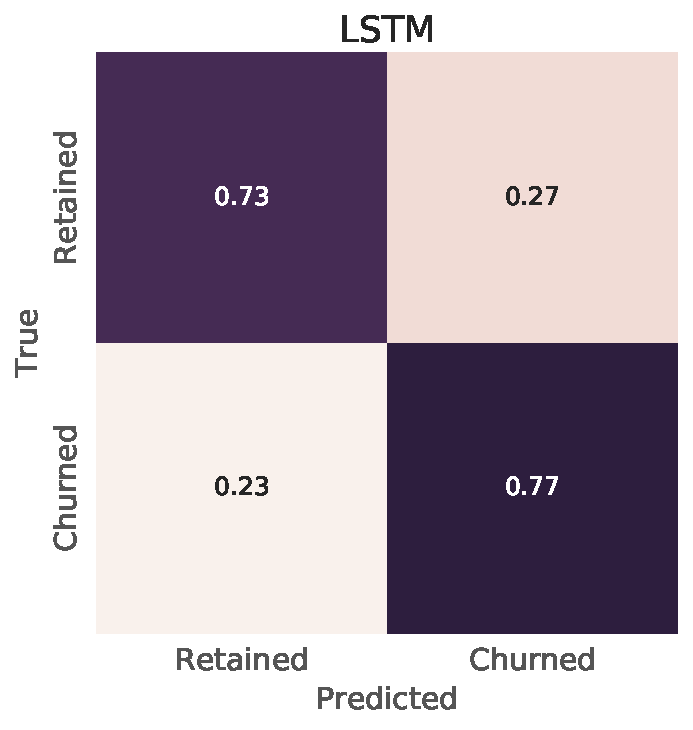
\includegraphics[width=0.5\textwidth,keepaspectratio]{figures/confusion_example.pdf}
    \caption{An example of a normalized confusion matrix}
    \label{fig:confusion_example}
\end{figure}

The confusion matrix is an excellent visualization tool to estimate the performance of a model. The values that should be maximized, the \emph{true positives} (TP) and \emph{true negatives} (TN), represent the samples that were correctly labeled as possessing the feature of interest or not, respectively. On the other hand, the \emph{false positives} (FP) and \emph{false negatives} (FN) are the misclassified samples where the algorithm predicted that the feature was present while in truth it was not and vice-versa. In this work, the positive class will always represent a churning user, and it follows that the negative class represents the non-churners.

\subsection{Classification Accuracy}

Several different metrics can be derived from the confusion matrix table. The \emph{classification accuracy} (CA) of a model is a common metric that corresponds to the fraction of the correctly classified samples on the test set, and can be calculated as follows:

\begin{equation}
CA = \frac{TP + TN}{TP + TN + FP + FN} 
\end{equation}

While trivial to understand, this metric may lead to erroneous conclusions when class imbalance is present in the test set, which is a common occurrence on the churn prediction domain. For example, if 9 out of 10 users of a dataset are non-churners, any classifier that simply outputs a negative class for all samples will result in an accuracy of 90\%, however its ability of detecting churners is non-existent. For a service provider, detecting churn cases is always more important than detecting the loyal users, and this metric by itself cannot represent this goal \citep{Burez2009} \citep{Hassouna2015}.

\subsection{Precision, Recall and Other Metrics}

To address the class imbalance problem of the classification accuracy, others metrics are also commonly used. The \emph{positive predictive value} (PPV, also known as precision) is the proportion of the samples labeled as positive which are true positives, and describes the performance of the algorithm. The \emph{true positive rate} (TPR, also called sensitivity and recall) of a model corresponds to the number of correctly predicted positive samples divided by all positive samples. \emph{True negative rate} (TNR, also called specificity and fall-out) is the number of correctly predicted negatives divided by all true negatives. The \emph{false positive rate} (FPR, also called false alarm ratio) is the probability of receiving a false positive as output of an experiment, and is calculated by dividing the number of false positives by the total number of positive samples. The \emph{F1 score} (F1, also called F-score or F-measure) builds upon precision and recall by returning an harmonic mean between these two metrics.

\begin{equation}
PPV = \frac{TP}{TP + FP}
\end{equation}

\begin{equation}
TPR = \frac{TP}{TP + FN}
\end{equation}

\begin{equation}
TNR = \frac{TN}{TN + FP}
\end{equation}

\begin{equation}
FPR = \frac{FP}{TN + FP} = 1 - TNR
\end{equation}

\begin{equation}
F1 = 2 \times \frac{PPV \times TPR}{PPV + TPR}
\end{equation}

Depending on the distribution of classes of the dataset, it is often difficult (although desirable) to maximize both precision and recall metrics at the same time. A compromise must be reached that achieves the best trade-off between the two, which is commonly a business decision.

\subsection{Receiver Operating Characteristic}

The \emph{receiver operating characteristic} (ROC) is a visualization tool that plots the relationship between the true positive rate (commonly the y-axis) and the false positive rate (the x-axis) of a binary classifier system. The curve is drawn by selecting different parameters of a model or levels of threshold for the decision boundary between the positive and negative classes. For example, when the output of a classifier is a probability value (like in logistic regression), different thresholds can be chosen to decide whether a user is a churner or not, depending if the goal is to minimize FPR or maximize TPR. An example of a ROC curve can be seen in Figure \ref{fig:roc_example}.

\begin{figure}[h]
    \centering
    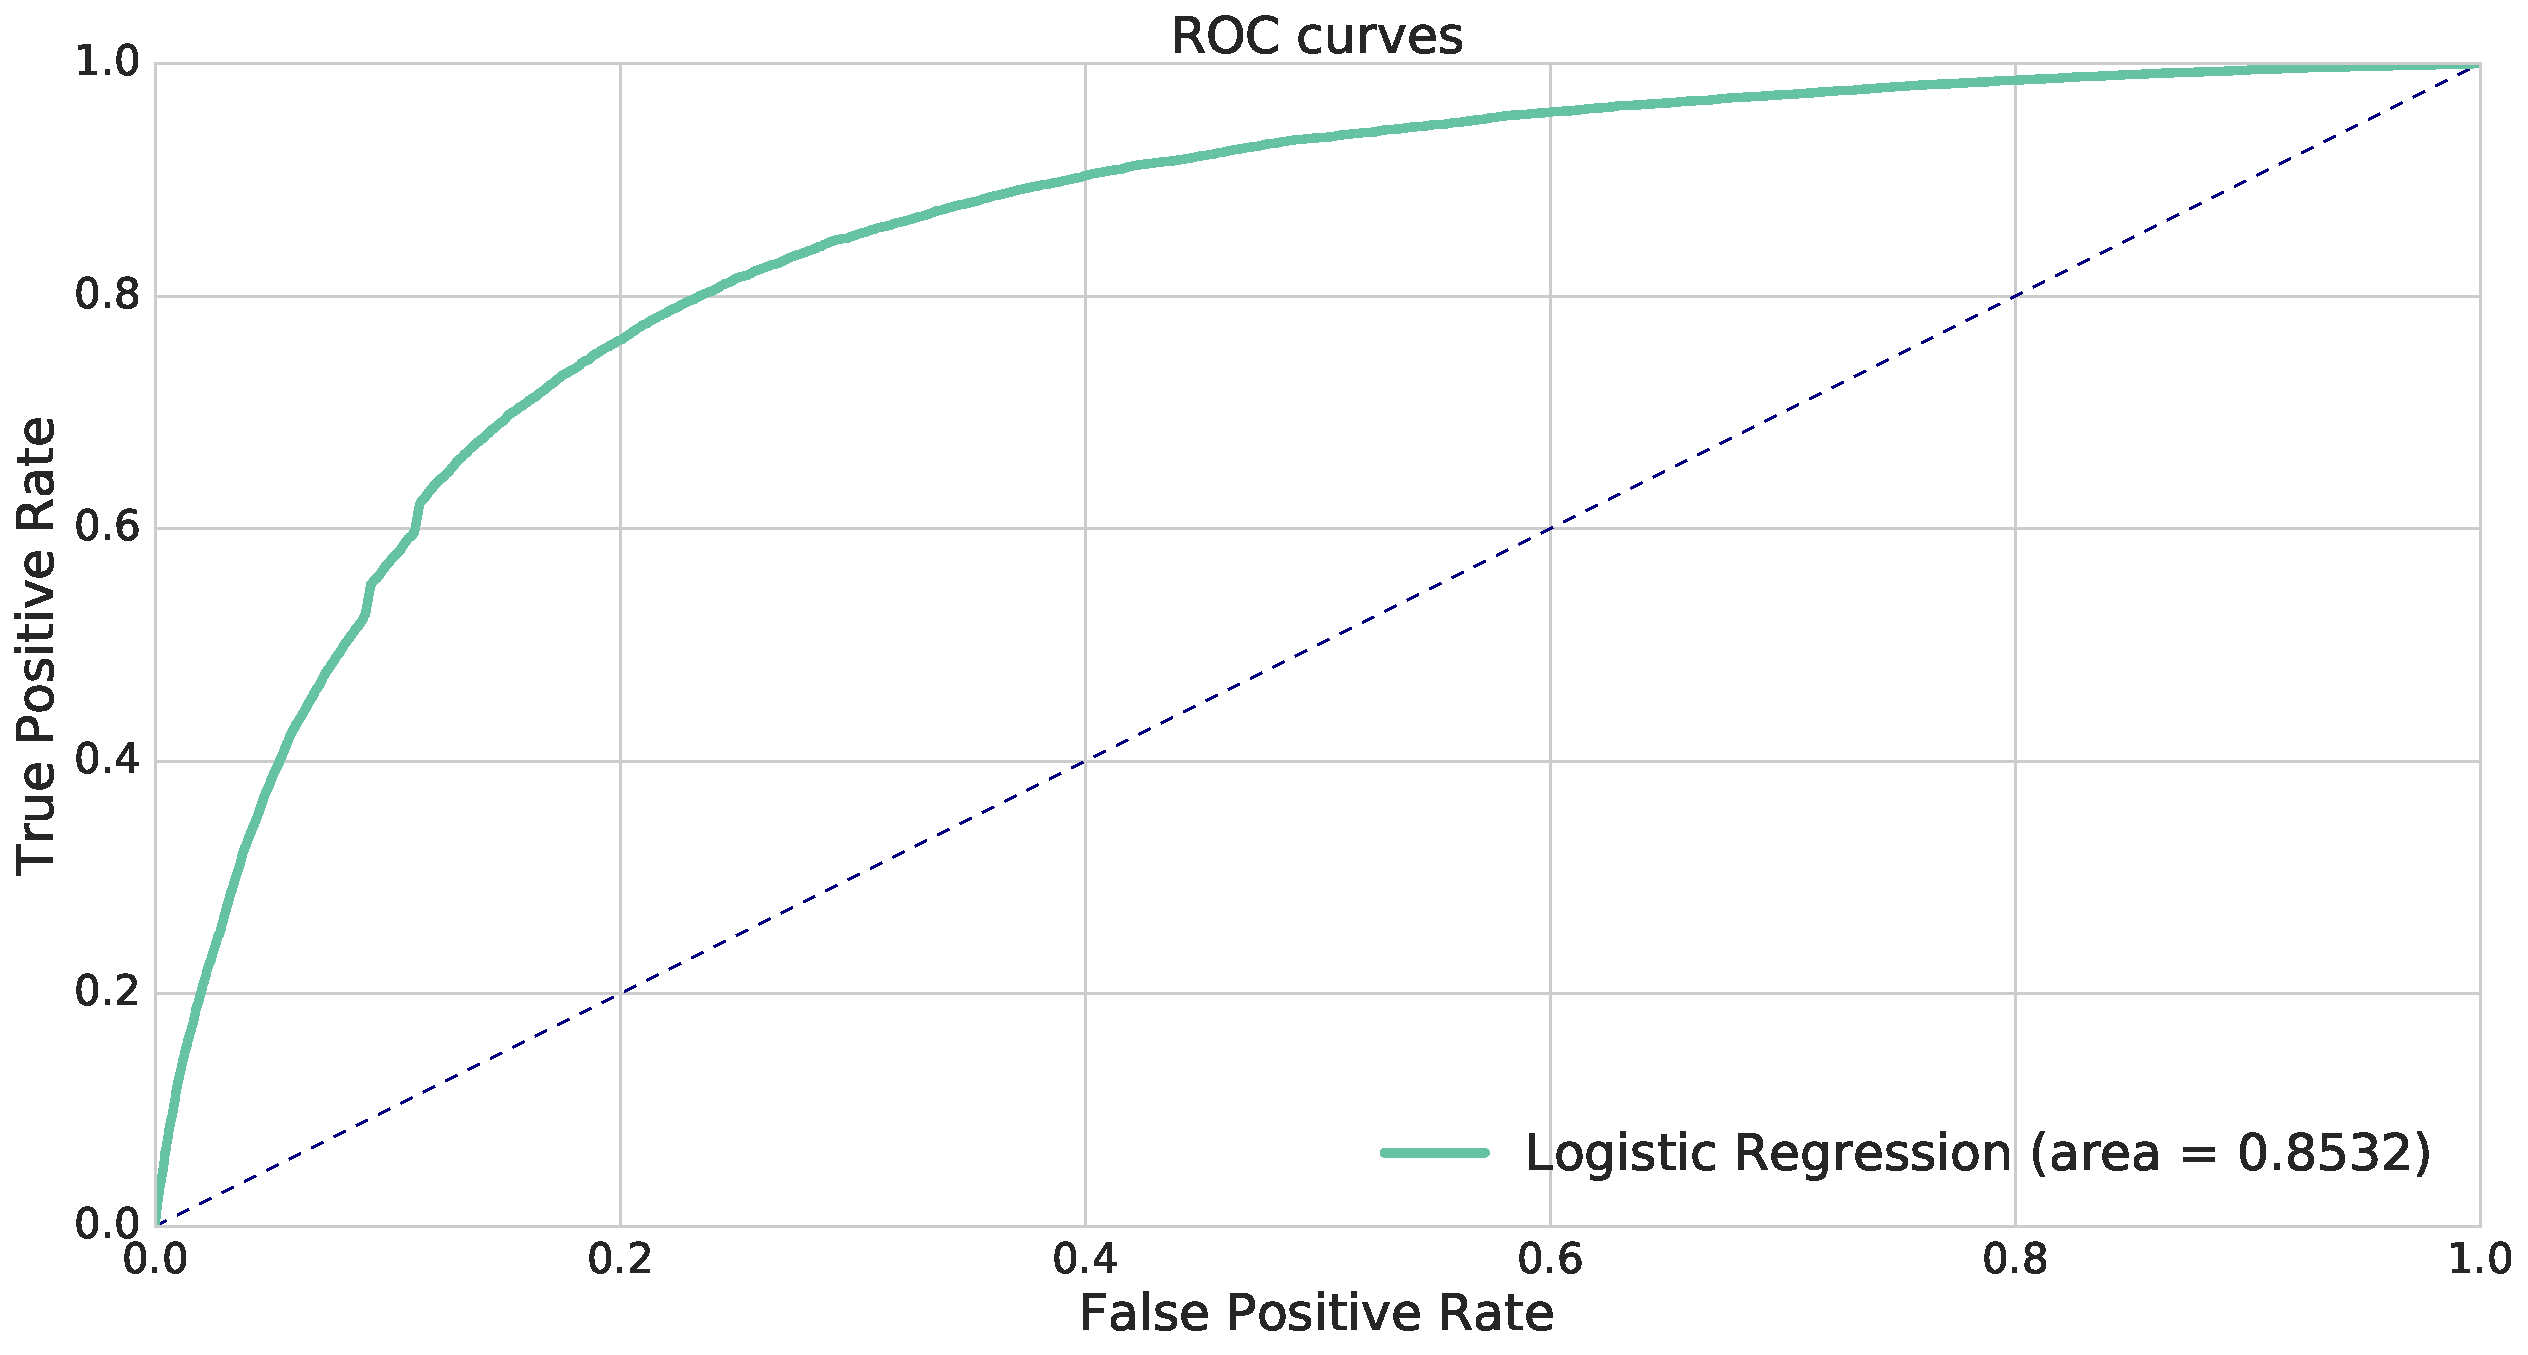
\includegraphics[width=1.0\textwidth,keepaspectratio]{figures/roc_example.pdf}
    \caption{An example of a ROC curve}
    \label{fig:roc_example}
\end{figure}

A good classifier would score values close to the upper-left corner of the plot, where the point (0,1) represents a perfect classifier with 100\% TPR and 0\% FPR. On the other hand, an algorithm that outputs a curve alongside the diagonal where TPR and FPR are almost the same at different threshold levels can be considered close to a random guess, like the flip of a coin. A classifier would underperform if its scores are closer to the bottom-right corner of the plot, however this result can always be mirrored by updating the model to simply invert the positive and negative labels of the classified samples.

ROC curves can be used to compare the performance of different models by measuring the \emph{area under the curve} (AUC) of its plotted scores, which ranges from 0.0 to 1.0. The greater this area, the better the algorithm is to find a specific feature. Moreover, models with an area close to 0.5 can be assumed to perform not much better than random guess, since this is the total area under the diagonal line. The AUC can also be interpreted as the probability of a randomly picked positive sample is ranked higher by the model when compared to a randomly picked negative case.

\subsection{Precision-Recall Curves}

While ROC curve is the most commonly used method for evaluating the performance of a classifier, it still fails to capture the true quality of the model when data is severely sparse. For any heavily skewed dataset, predicting the negative majority correctly can be accomplished easily, however the same cannot be said about the rare positive class. Since ROC curves utilizes the false positive rate calculated using the large number of true negatives, the plot may give the idea that the model is doing quite well, while failing to show its ability to predict the positive class. 

Visualizing the precision plotted against its recall value may be more informative when dealing with sparse data. The \emph{precision-recall curve} is the visualization tool that accomplishes exactly that, for every threshold value, the recall (commonly the x-axis) is plotted against its precision (the y-axis). 

\Cref{fig:prc_example} shows an example a precision-recall curve plotted for the same data from \Cref{fig:roc_example}, however focusing only in the churning class which is the focus of this study. Here we can clearly see how the precision is affected by an skewed dataset: even if our model manages to have only a small fraction of false positives, since they are many the precision will quickly be reduced.

\begin{figure}[h]
    \centering
    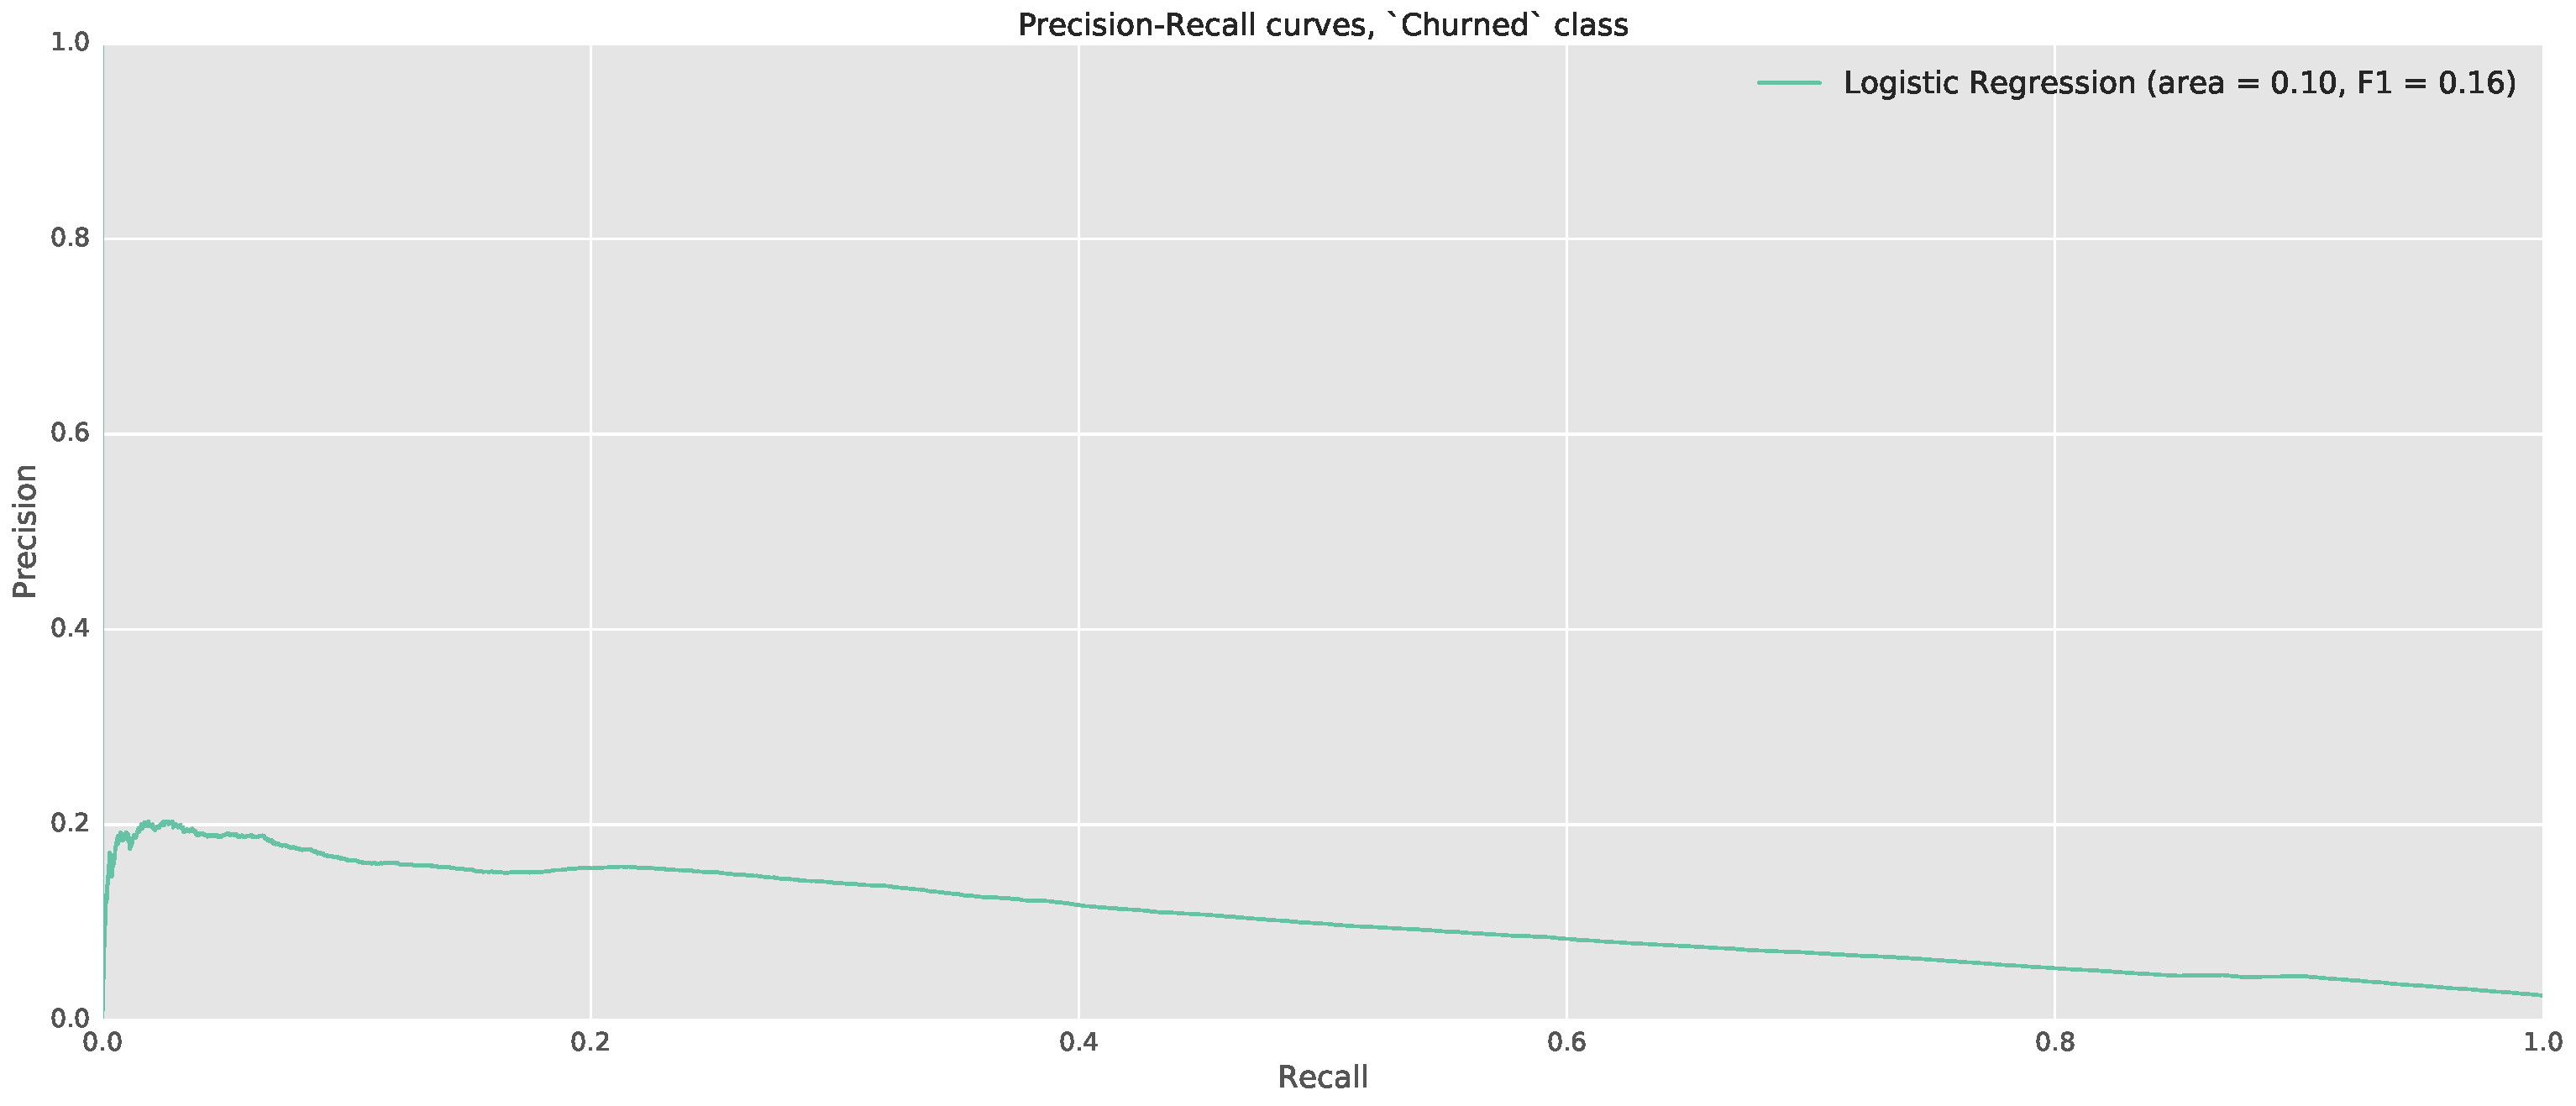
\includegraphics[width=1.0\textwidth,keepaspectratio]{figures/prc_example.pdf}
    \caption{An example of a precision-recall curve}
    \label{fig:prc_example}
\end{figure}

Similarly to ROC curves, the area under the line correlates to the overall quality of the classifier: values closer to 1 indicates that a model has high precision and recall for every different tested threshold.  The balance between precision and recall can be manipulated by changing the threshold value: if we want to increase the recall, simply using a lower threshold will yield an increase in the number of true positives, at the cost of lower precision.

\section{Software and Libraries}

The experiments on this thesis were only made possible by utilizing well known open-source software libraries for data processing and machine learning. The recurrent LSTM models were implemented in Keras \citep{chollet2015keras}, a high-level deep learning wrapper library written in Python.  Tensorflow \citep{abadi2016tensorflow}, a library for numerical computation using data flow graphs created by Google, was used as a backend for Keras. Random forests and logistic regressions models, as well as  the procedures for handling cross-validation and hyperparameter search, were implemented on Scikit-Learn \citep{scikit-learn}, a Python module for machine learning. The random undersampling was performed using a modified version of a library called Imbalanced-Learn \citep{lema2017imbalanced}, a Python package that offers several re-sampling techniques for imbalanced datasets. 

\chapter{Results}
\label{cha:results}

\epigraph{Talk is cheap. Show me the code.}{\textit{Linus Torvalds}}

This chapter will be dedicated to detail the experiments performed in this project, while also presenting the obtained results.

The experiments in this project aim to assess how the commonly used existing approaches for predicting churn performs comparing to a newer approach, LSTM. In addition, this chapter investigates how the scores of predictive models can be influenced and also explore how can we influence the scores of our predictor by changing different aspects of the input data. The experiments in this project are:

\begin{itemize}
\item Comparing LSTMs to baseline models commonly used for churn prediction
\item Measuring the performance change when varying the size of the prediction and observation windows for LSTM and the baseline models.
\item Experimenting on training models with different ratios between the churning and retaining classes, while analyzing their influence in classification accuracy.
\item Examining if applying methods such as dimensionality reduction can improve the performance of the predictive models.
\end{itemize}

The experiments will be briefly discussed in this chapter, a more insightful conversation shall be presented on \Cref{cha:discussion}. Several experiments and evaluations have been performed in this project work, each one resulting in a substantial amount of data that is too extensive to present in a single chapter. Therefore, the main results will be focused in this chapter, however additional extensive results can be thoroughly analyzed in \Cref{cha:add_results}.

The following explains details on the experimental setup and evaluation.

\begin{itemize}
\item The precision, recall and F1-score metrics were all obtained by thresholding the output scores to 50\%, which makes no assumption of whether the provider would rather decrease precision in favor of recall or vice-versa. Precision-recall and ROC curves plot however its corresponding metrics against all possible thresholds.
\item All experiments undersample the training data to a 1-to-1 ratio between churning and retaining users, unless otherwise stated.
\item In the experiments presented in this chapter the observation window is set to 56 days and the prediction window is 30 days, unless otherwise stated.
\item Random forest and logistic regression were trained using the SPTD version of the dataset defined in \Cref{sec:timewindows},  while LSTM was trained using MPTD.
\end{itemize}

\section{LSTM vs. Baseline Models}

In this experiment, our goal is to test the performance of the LSTM model compared to more established approaches for churn prediction. The pilot study has revealed that logistic regression and random forests are algorithms that are still fairly used in the industry and academia.

All three models were trained int the dataset composed of 56 days in the observation period and 30 days of prediction, where the training data is balanced as to have an equal number of churning and retaining samples.

The results for this experiment shows that LSTM has the largest scores of the evaluated models for almost all metrics in \Cref{tab:temporal_static}. LSTM shows a significant increase of F1-score of both classes when compared to logistic regression. It must be noted however that the difference to random forest is very slim, a model which is significantly faster to train and optimize. The difference may also be caused by random noise in our data, so the models may be considered comparable at best. Further discussion will be presented on \Cref{sec:dis_lstm_baseline}. 

\begin{table}[H]
\centering
\begin{tabular}{llrrrr}
\toprule
     &          &  F1-Score &    PR AUC &  Precision &    Recall \\
\midrule
\multirow{2}{*}{LSTM} & Retained &  \textbf{0.899} &  \textbf{0.994} &   \textbf{0.992} &  \textbf{0.821} \\
     & Churned &  \textbf{0.170} &  0.185 &   \textbf{0.096} &  \textbf{0.747} \\
\cline{1-6}
\multirow{2}{*}{Random Forest} & Retained &  0.895 &  \textbf{0.994} &   \textbf{0.992} &  0.816 \\
     & Churned &  0.164 &  \textbf{0.196} &   0.092 &  0.737 \\
\cline{1-6}
\multirow{2}{*}{Logistic Regression} & Retained &  0.830 &  0.993 &   0.991 &  0.714 \\
     & Churned &  0.115 &  0.104 &   0.062 &  0.747 \\
\bottomrule
\end{tabular}
\caption{Metrics for the LSTM vs. baseline experiment. Values in bold indicates the best performing classifier for each evaluation measure.}
\label{tab:temporal_static}
\end{table}

Another property that can be observed is that even though the accuracy for the retained class is deemed acceptable for all classifiers, the same cannot be stated about the performance of models for the churning users. The challenges of detecting a class label which is a vastly outnumbered by its counterpart reflects on the low precision scores obtained in this experiment. The undersampling performed on the training set bias the models to classify more users as churners than there is on the dataset, increasing the recall metric. However, even if a small fraction of the total negative samples are false positives, since there are many more retained users the precision is quickly reduced. The class imbalance and its impact in precision can be seen in the confusion matrices in \Cref{fig:cfm_temporal_static}. The influence of class distribution motivated the experiment performed in \Cref{sec:exp_class_dist}, where the results will be fully discussed in \Cref{sec:dis_class_dist}.

\begin{figure}[H]
    \centering
    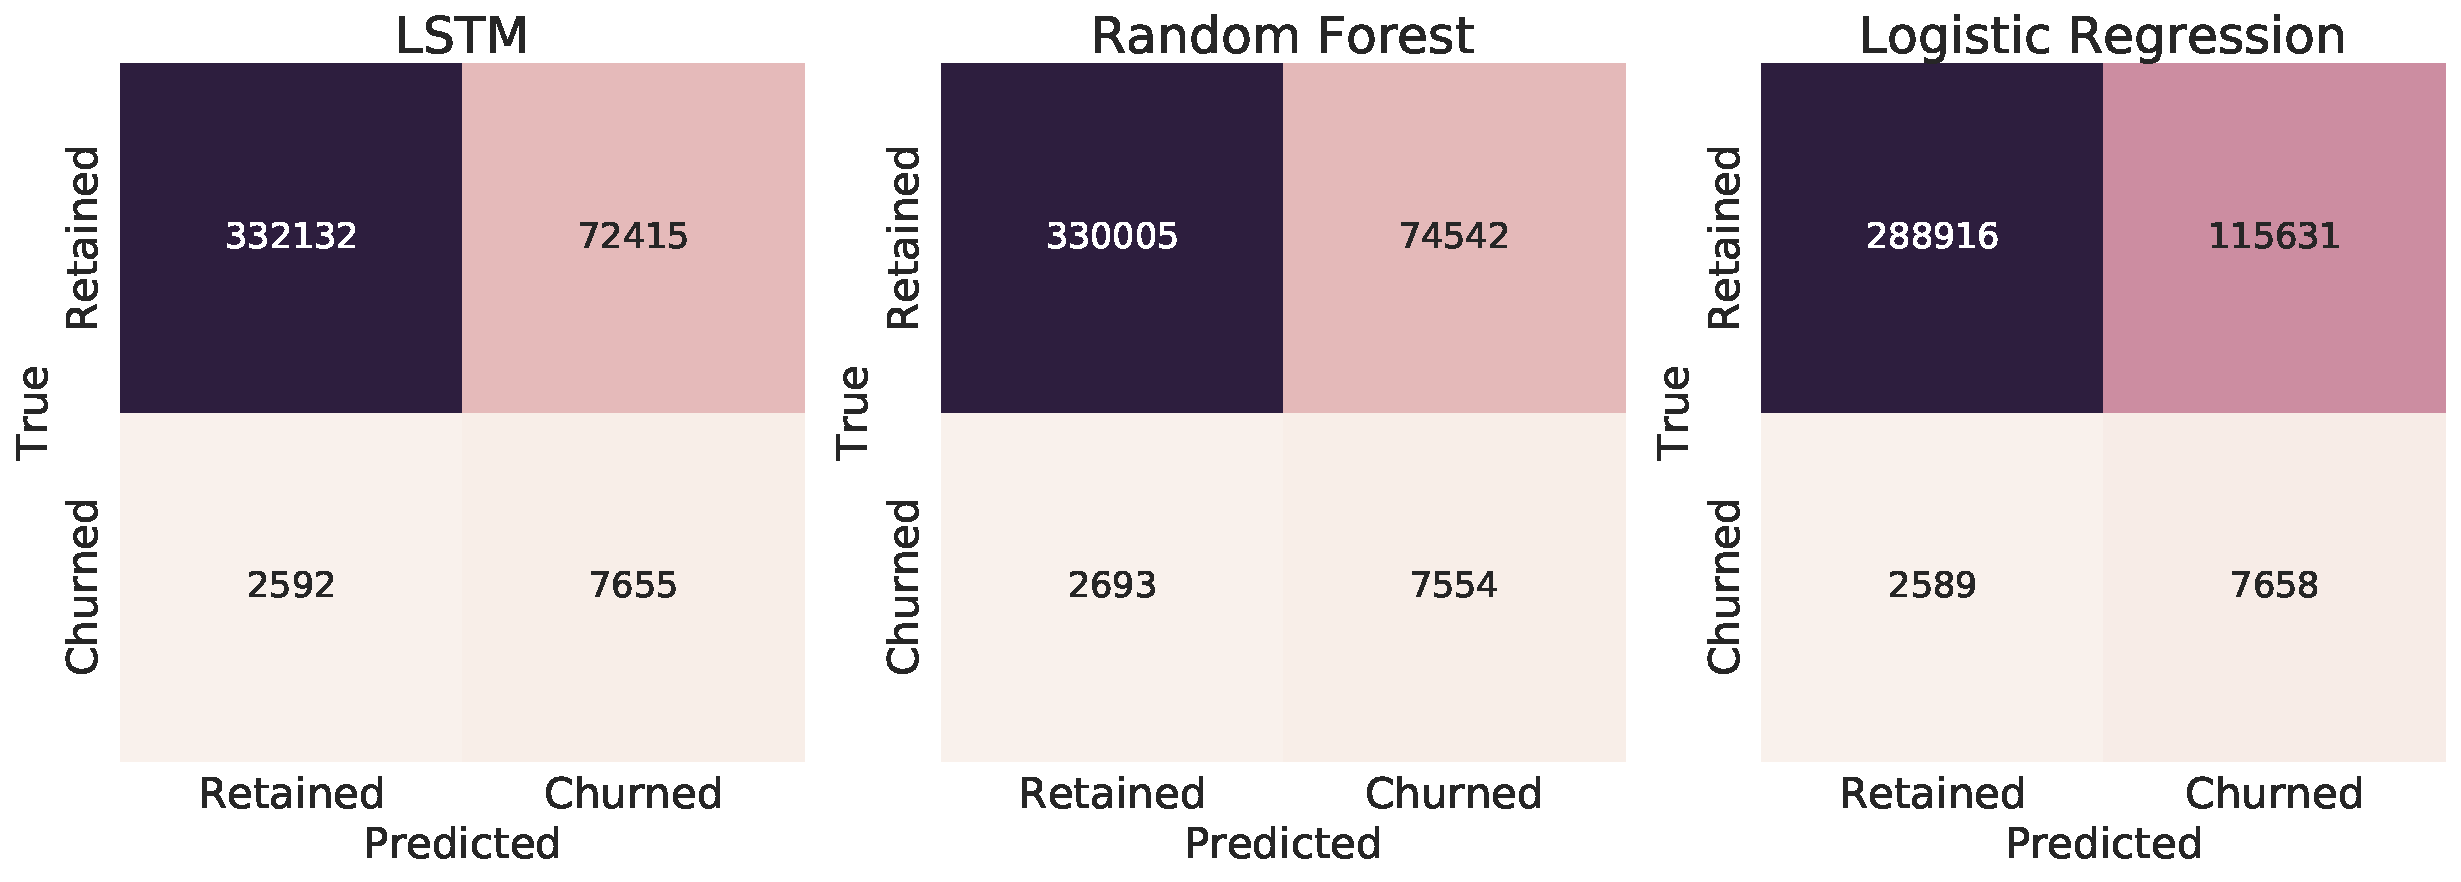
\includegraphics[width=1.0\textwidth,keepaspectratio]{figures/cfm_temporal_static.pdf}
    \caption{Confusion matrices for the LSTM and baseline models}
    \label{fig:cfm_temporal_static}
\end{figure}

\Cref{fig:prc_temporal_static} plots the precision-recall curves of the churned class for the LSTM and the evaluated baseline models for several different threshold levels. The first property that can be seen is how quickly precision decreases as recall is increased: precision drops to $0.4$ in the top classifiers before even reaching recall of $0.1$, which is, as discussed previously, the result of the imbalanced data used for testing.  

Additionally, the similarity between LSTM and random forests is expressed in the overlapping precision-recall curves. Random forests exhibits a slightly better precision for recall scores lower than $0.6$, being overtaken by the LSTM model beyond this point by a small margin. The gap in performance between logistic regression and the top classifiers is further visualized in these plots, suggesting that this model might not be a good choice for predicting churn for this specific dataset. The recall of approximately $0.9$ is the converging point where all curves meet, being the probability threshold at this level so low that most samples are equally classified as churning for every different model.

\begin{figure}[H]
    \centering
    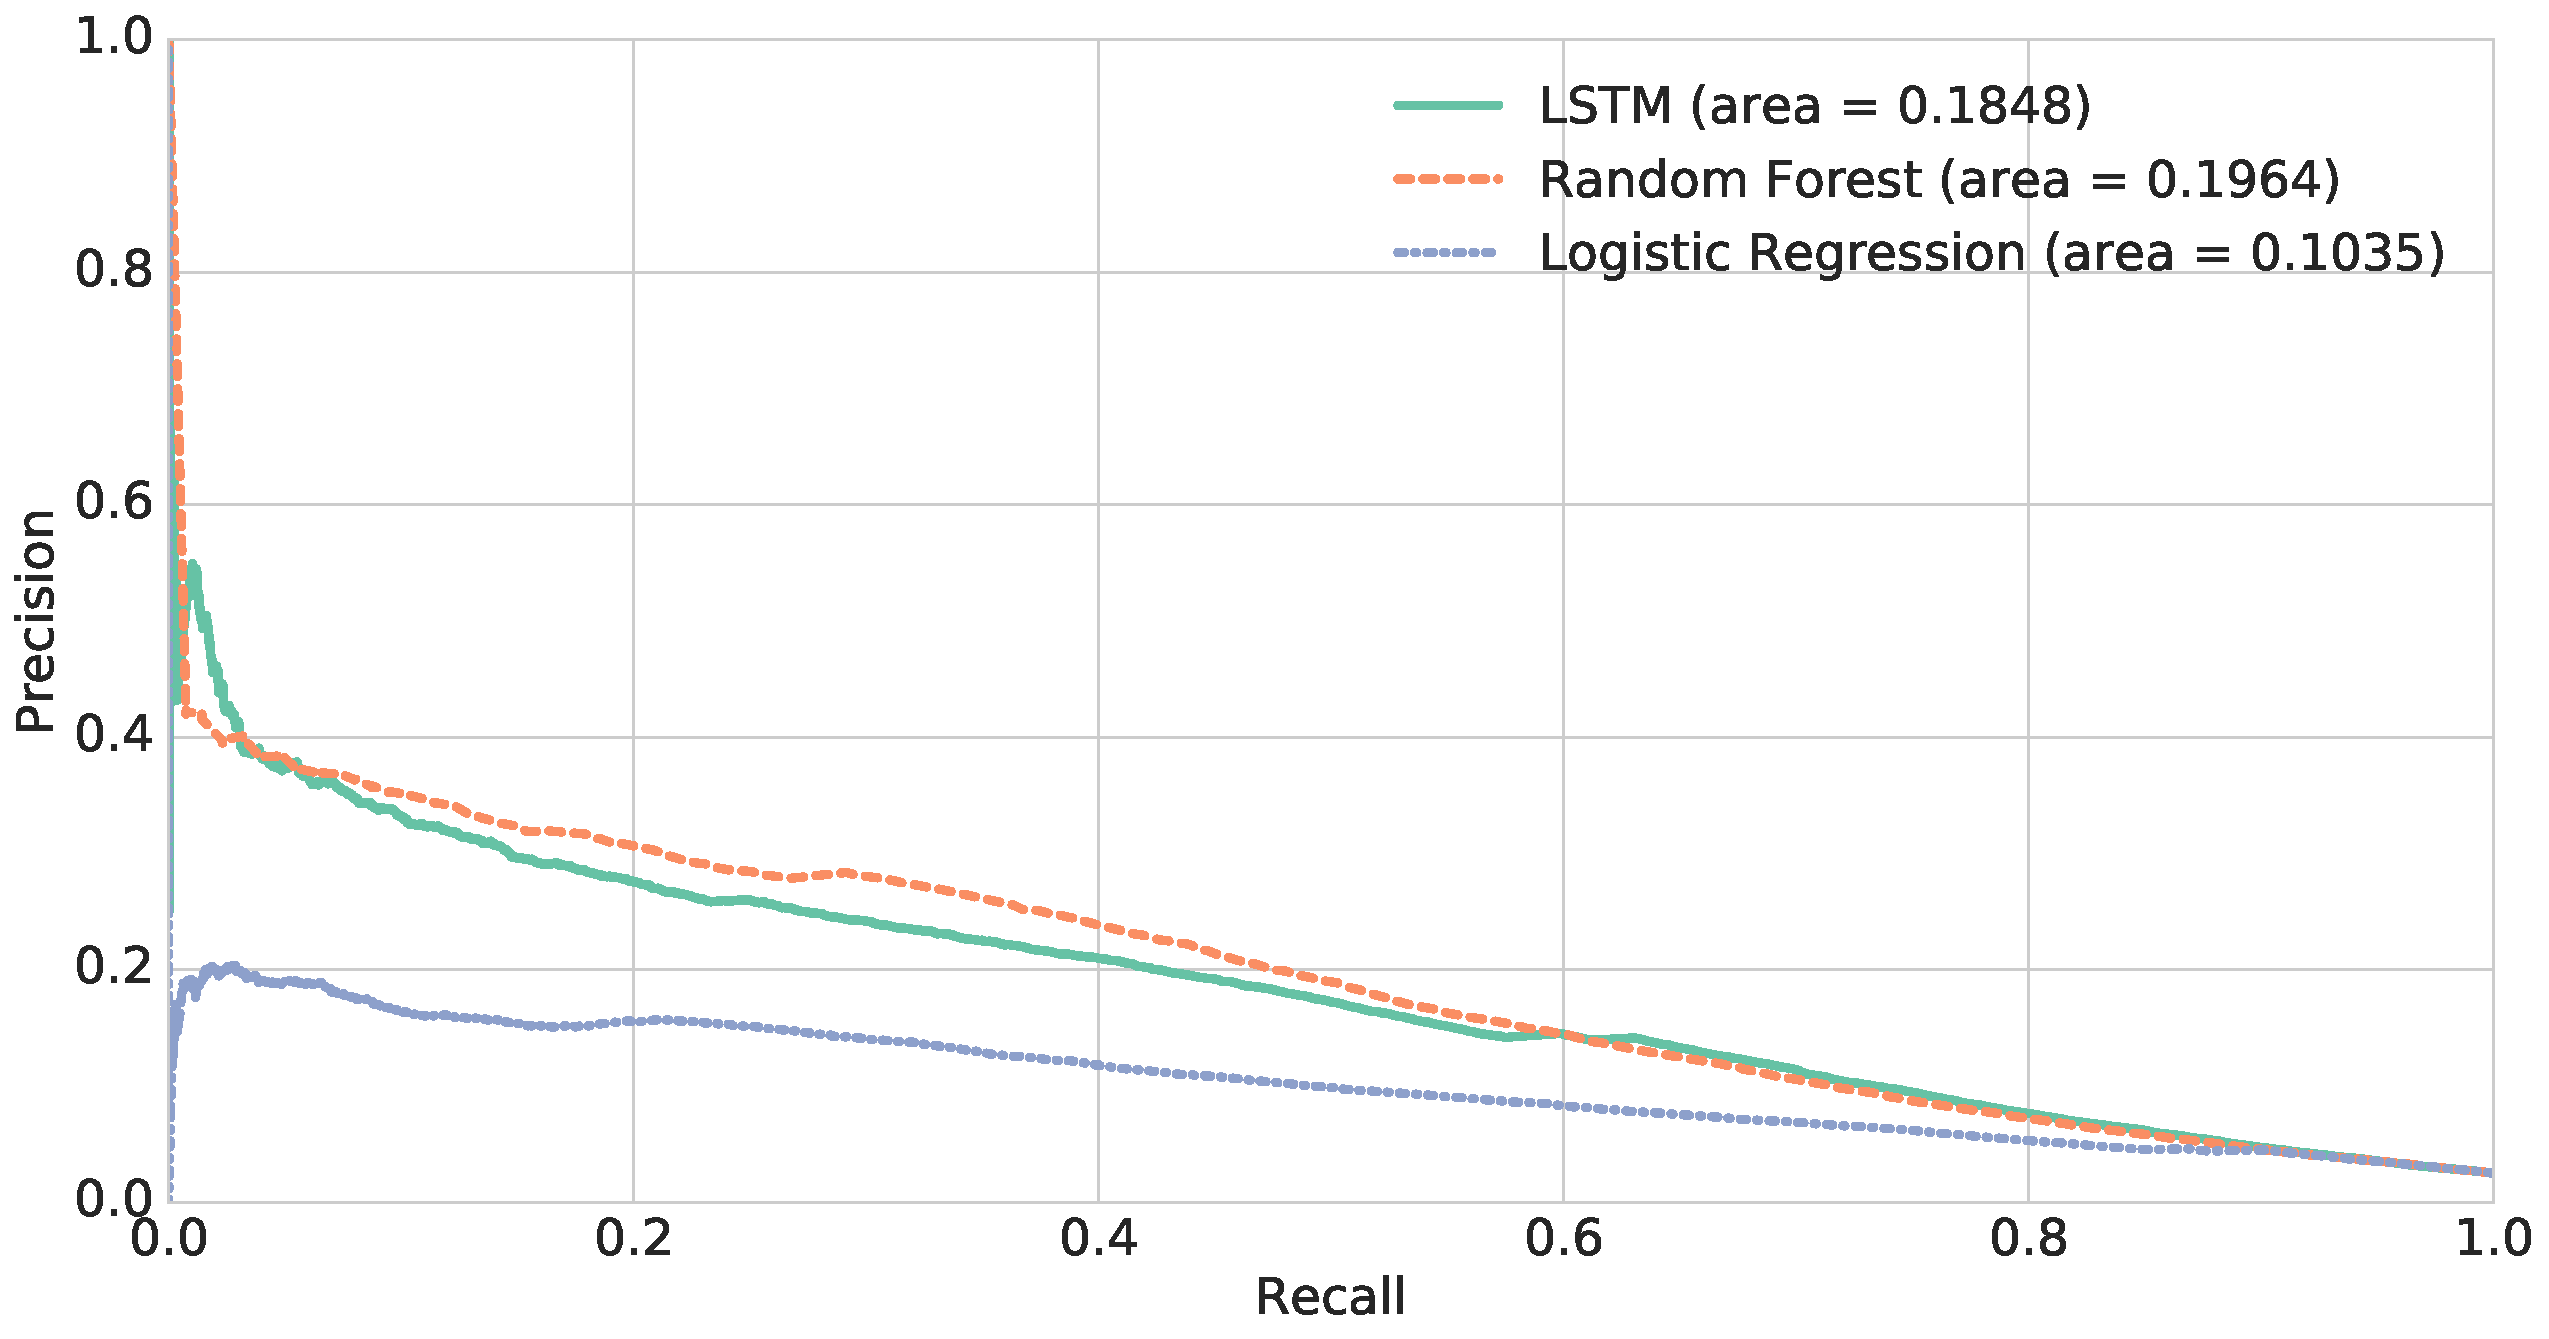
\includegraphics[width=1.0\textwidth,keepaspectratio]{figures/prc_temporal_static.pdf}
    \caption{Precision-recall curves of the churned class for the LSTM and baseline models}
    \label{fig:prc_temporal_static}
\end{figure}

\Cref{fig:roc_temporal_static} plots the ROC curves for LSTM and the baseline models for the same experiment. Here it can be seen that ROC diminishes the differences between predictions of LSTM and random forest, the disparity between models around the converging point of $0.6$ recall (or true positive rate) can hardly be noticed. Also it must be said ROC curves are insensitive to class balance: since the true positive and false positive rates are label independent from each other and normalized, the total number of examples between each class exerts no influence on the plot \citep{fawcett2004roc}. Precision-recall curves proves to be a better visualization tool when datasets are heavily skewed \citep{saito2015precision}.

\begin{figure}[H]
    \centering
    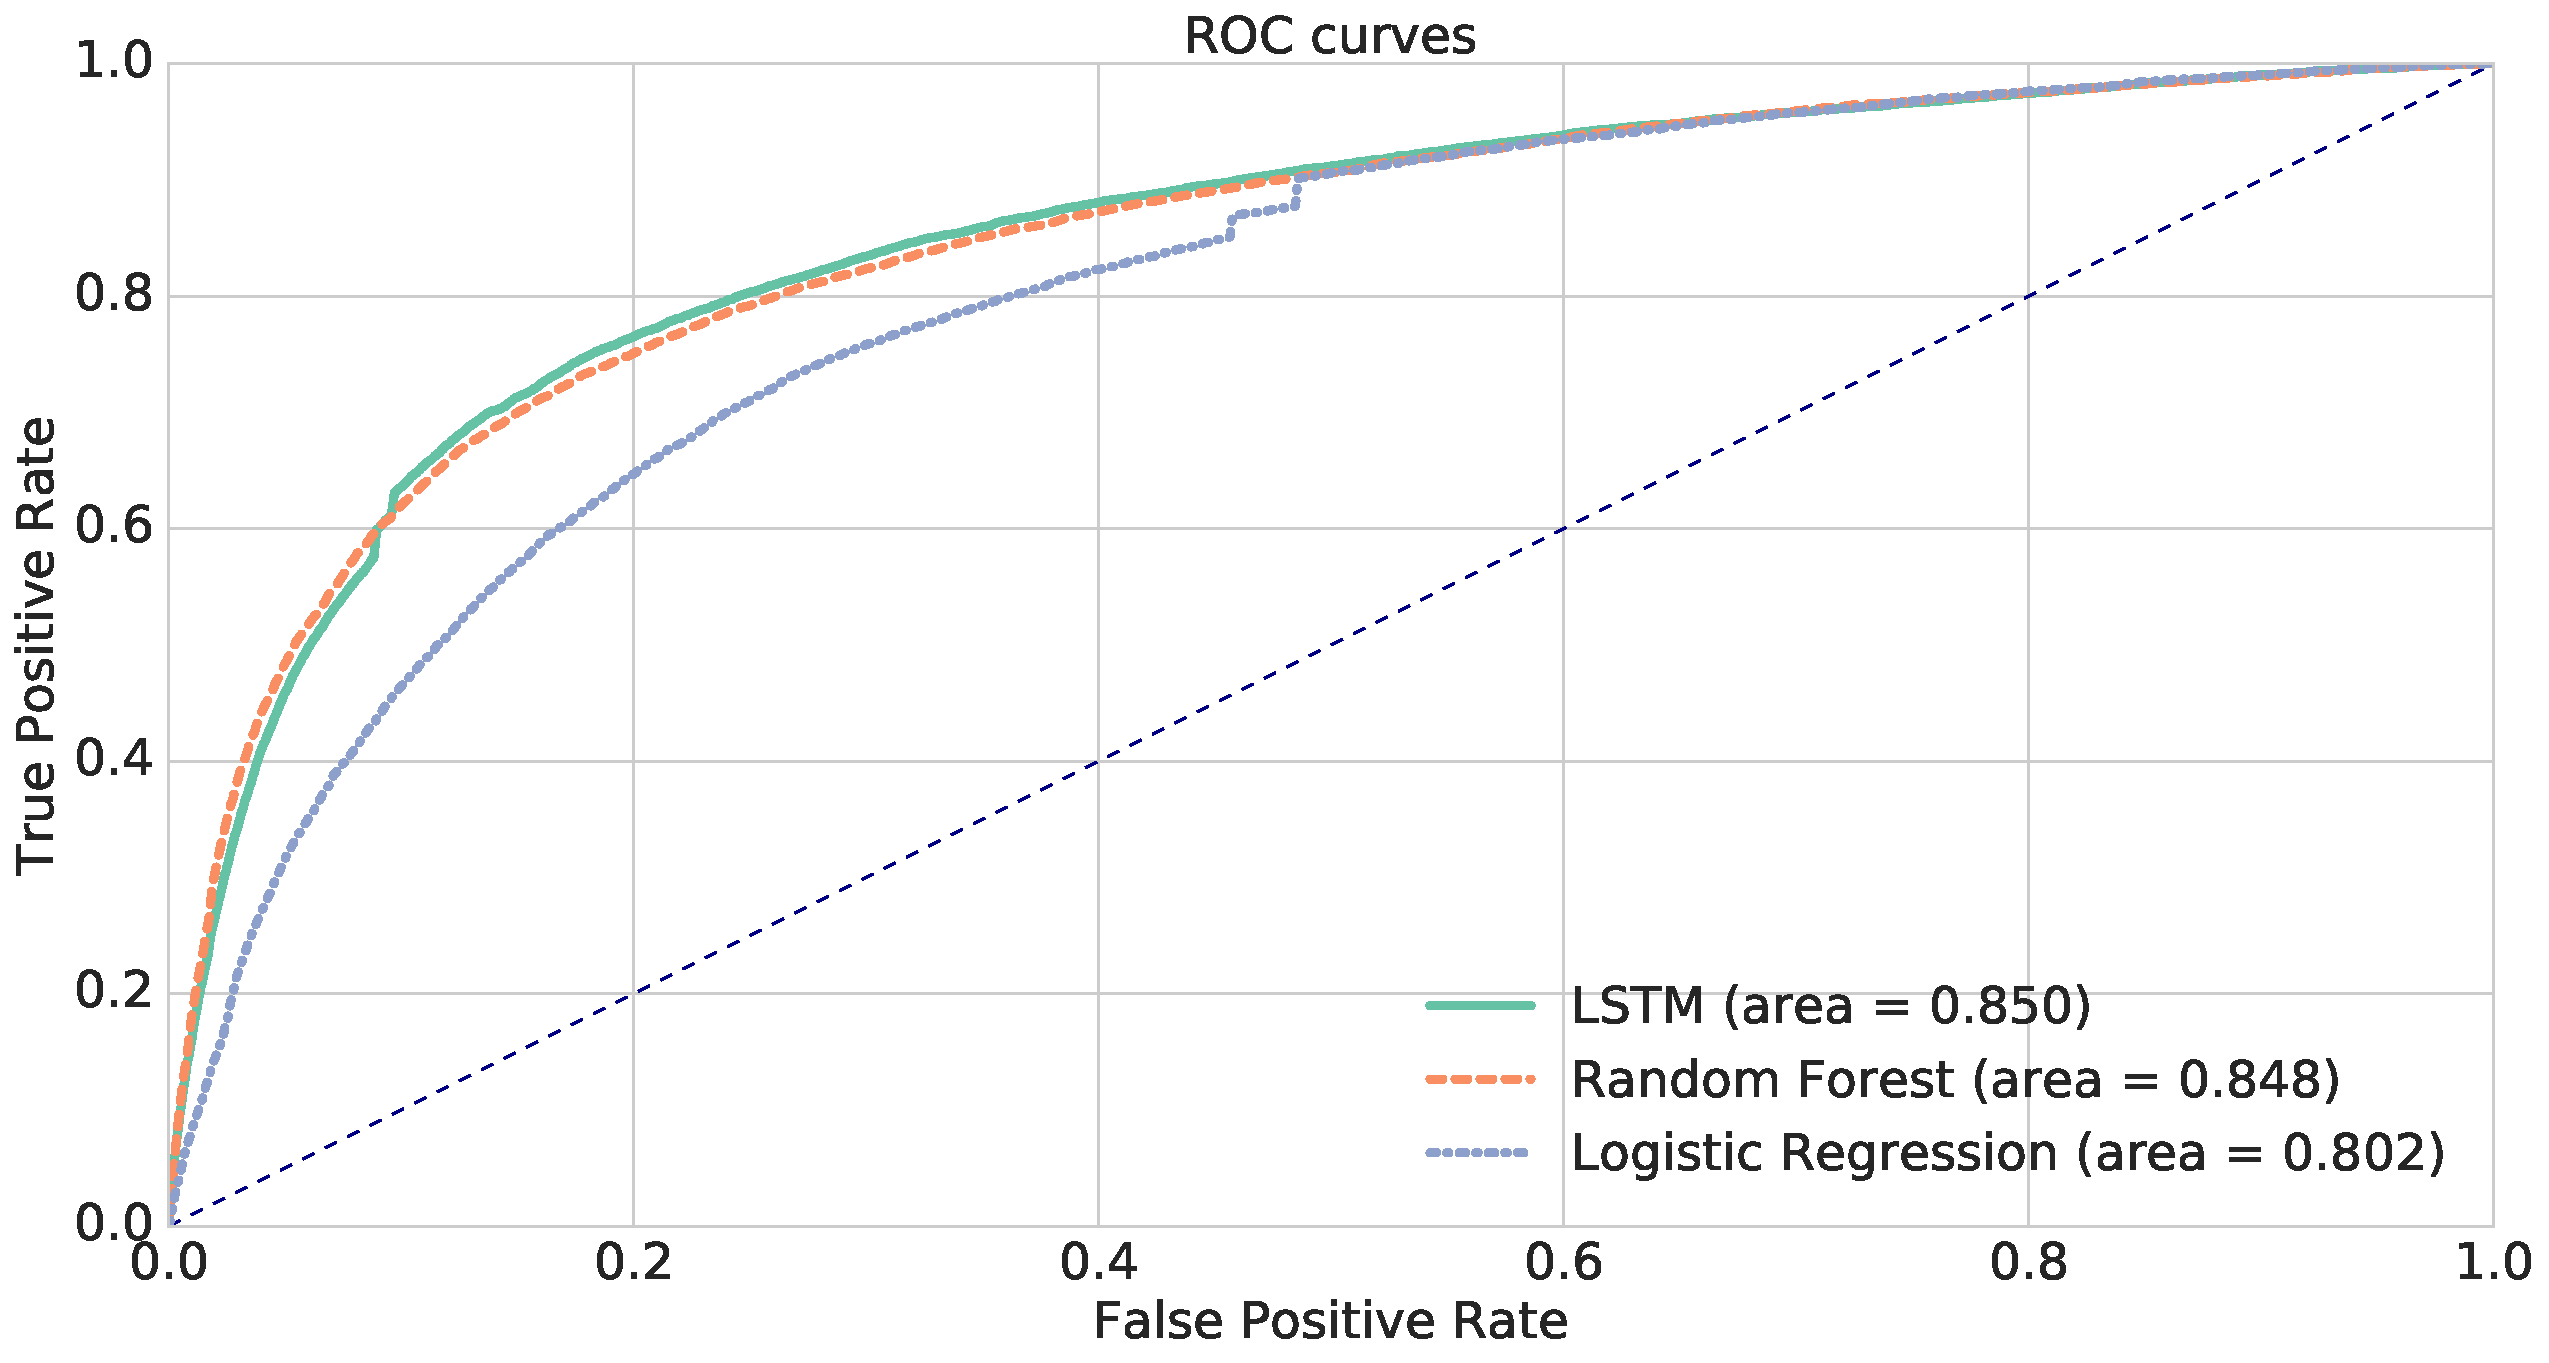
\includegraphics[width=1.0\textwidth,keepaspectratio]{figures/roc_temporal_static.pdf}
    \caption{ROC curves for the LSTM and baseline models}
    \label{fig:roc_temporal_static}
\end{figure}


\section{Experimenting on Different Window Sizes}

The size chosen for the time windows has an influence on the performance metrics of our trained estimators that is non-trivial to anticipate. In the following set of experiments, we investigate the impact of the observation window and prediction window on the quality of all evaluated classifiers. Our hypothesis is that a larger observation window should improve the quality of LSTM by exposing the model to temporal patterns over a wider period of time. The investigation on the prediction window size will help us to assess for how long in future classifiers can predict user churn with a reasonable accuracy. 

\subsection{Observation Window}
\label{sec:exp_obs_window}

Different sizes for the observation window correlates to how much historical data of customers is going to be used for model training. A large observation window indicates that the training data will look further in the past and be composed of more data points, while a small window indicates that less historical information is fed into classifiers. It is expected that with more data, a better classification accuracy can be achieved, and is expected that LSTM will display a greater improvement by being exposed to more temporal patterns of the user behavior. The main question that this experiment is thus exploring is which models benefit the most by having more historical customer data for training, which is a topic thoroughly explored in the work of \citep{Ballings2012}.

Our experiment involved increasing the size of the observation window by 7 days and training a model for each, evaluating the performance of each. The prediction window is made constant at 30 days, corresponding to the same period in time for all different parameters tested in this experiment. 

The results of this experiment when considering the churning class can be seen in \Cref{fig:line_obs_window}. Both random forest and logistic regression models exhibit an increase in F1-scores when the size of the observation window is made larger, with a relative performance gain of $19\%$ and $18\%$ respectively when comparing the best and worst configurations. The LSTM model on the other hand show a rather erratic behavior, reaching its top when the window is sized at 49 days, obtaining $36\%$ of maximum improvement instead. LSTM also exhibits a higher F1-score gain than the other models when the observation window is increased, indicating that a larger accuracy can be achieved if more historical user data is available. 

\begin{figure}[H]
    \centering
    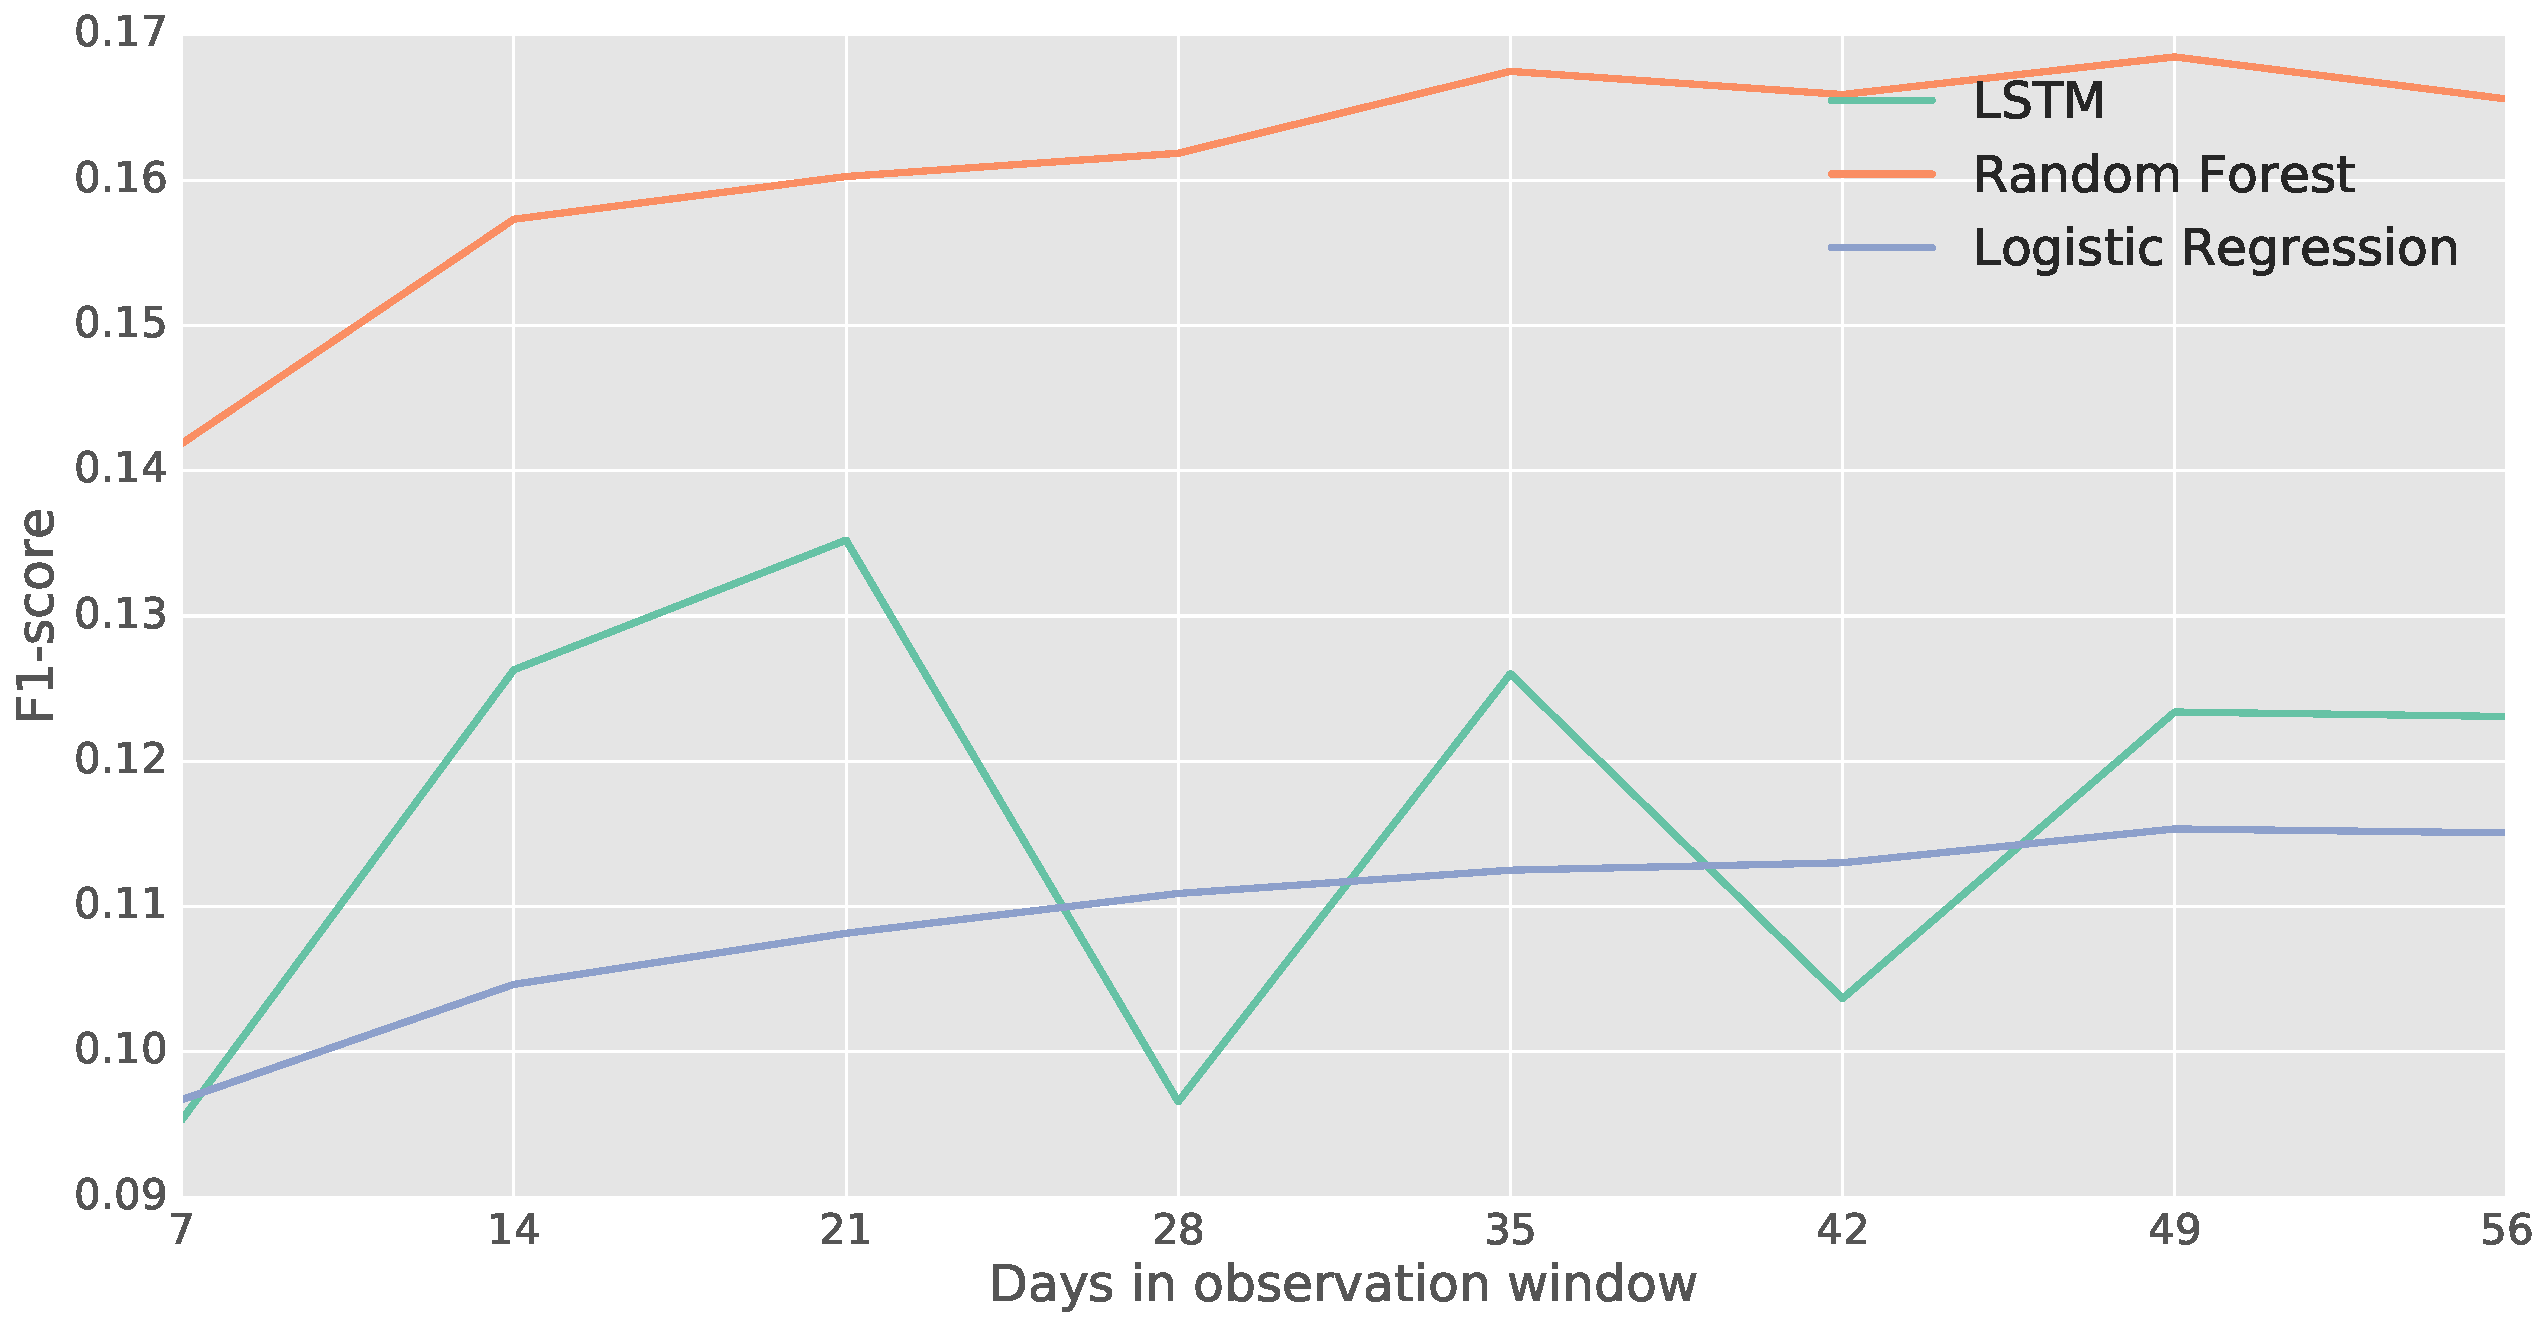
\includegraphics[width=1.0\textwidth,keepaspectratio]{figures/line_obs_window.pdf}
    \caption{F1-scores for the churned class using different observation window sizes and models}
    \label{fig:line_obs_window}
\end{figure}

As can be seen in \Cref{fig:line_obs_window_ret}, the performance of predictions for the retained class also exhibits a trend of increasing when more historical data is added to training, however at a smaller magnitude. Random forest and logistic regression obtain a relative increase in F1-score of $3\%$ and $2\%$ respectively between the best and worst configurations tested, while LSTM obtains a slight larger relative gain of approximately $5\%$.

\begin{figure}[H]
    \centering
    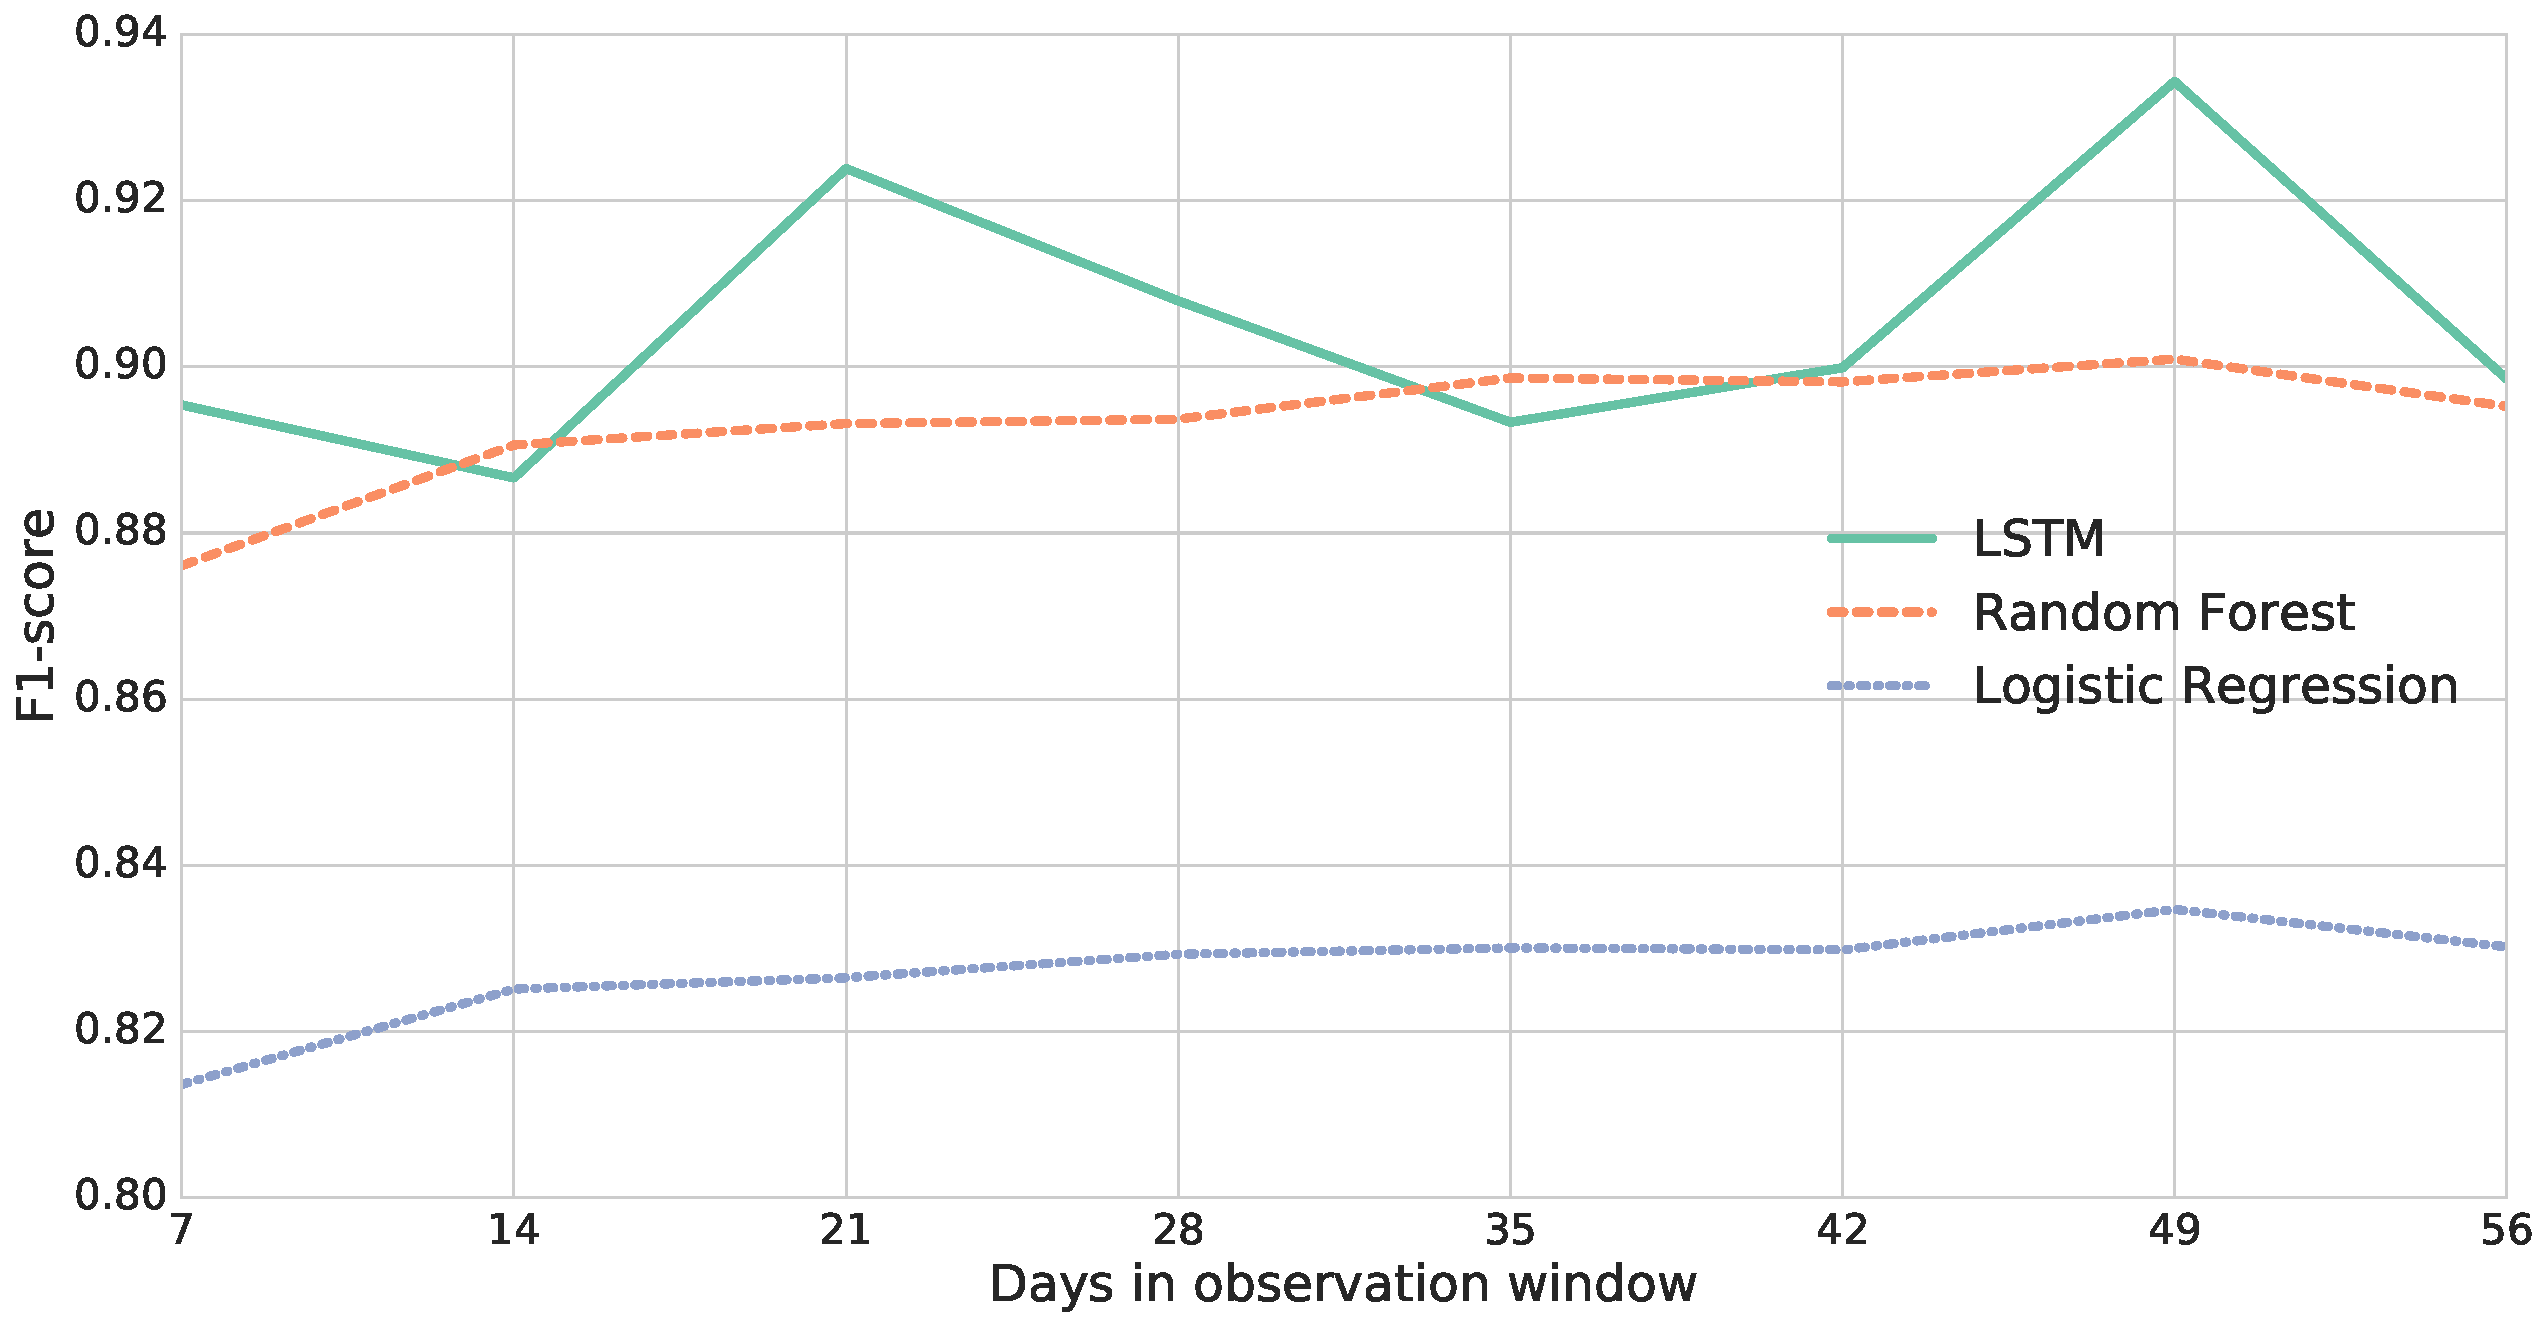
\includegraphics[width=1.0\textwidth,keepaspectratio]{figures/line_obs_window_retained.pdf}
    \caption{F1-scores for the retained class using different observation window sizes and models}
    \label{fig:line_obs_window_ret}
\end{figure}

Precision-recall curves, ROC curves and metrics table for this experiment can be seen in \Cref{fig:prc_obs_window}, \Cref{fig:roc_obs_window} and \Cref{tab:obs_window}, respectively.

\subsection{Prediction Window}

Modifying the size of the prediction window indicates how strict we are for considering a user a churner or not. Small windows are commonly used for services lacking a formal contract between the provider and the customer, which is similar approach used in the works of \citep{Dror2012}, \citep{Runge2014} and \citep{Pudipeddi2014}. Larger prediction window sizes are often seem in "classical" service providers like the telecom industry where a contract is commonly established, an approach that is widely seem in the churn prediction literature, \citep{Khan2015} and \citep{Hassouna2015} to name a few. 

In the experimentation setup of this project, changing the prediction window size will only affect which label will be set for each customer in the dataset. Smaller windows indicates that we are more strict for considering a user as retained, requiring that content is streamed in a shorter period of time and increasing the amount of churners. Larger windows will have the opposite effect: less users will be classified as churners since the time period where a stream will be looked up for as to consider him active or not is larger. This experiment thus explores how far in the future classifiers can predict with a reasonable accuracy, which is accomplished by analyzing how the performance is affected by estimating the user label over increasing periods of time in the future. 

This experiment involves evaluating the performance of classifiers for different sizes of the prediction window. The size of the window is initially set to 7 days, incrementally increasing it in intervals of 7 days up to the maximum size of 28 days. The size of the observation window is kept constant at 56 days, corresponding to the same period in time. It is important to note that smaller window sizes means that a larger share of users will be considered churners, and since the training data is undersampled to 1-to-1 ratio between classes the number of samples will be larger. 

The result of this experiment for the churning users can be seen in \Cref{fig:line_pred_window}. Both LSTM and random forests exhibit top F1-scores when the prediction window is smallest in size, with a relative increase of approximately $73\%$ and $86\%$ respectively between the best and worst configurations. The  performance of both models gradually decreases as more days are added to the window. Two reasons for this behavior can be inferred: first, smaller window means more churners, and due to undersampling this means more training data. Second, it is easier to predict what the user is going to do right after the last observed data point when compared to further days in the future. 

\begin{figure}[H]
    \centering
    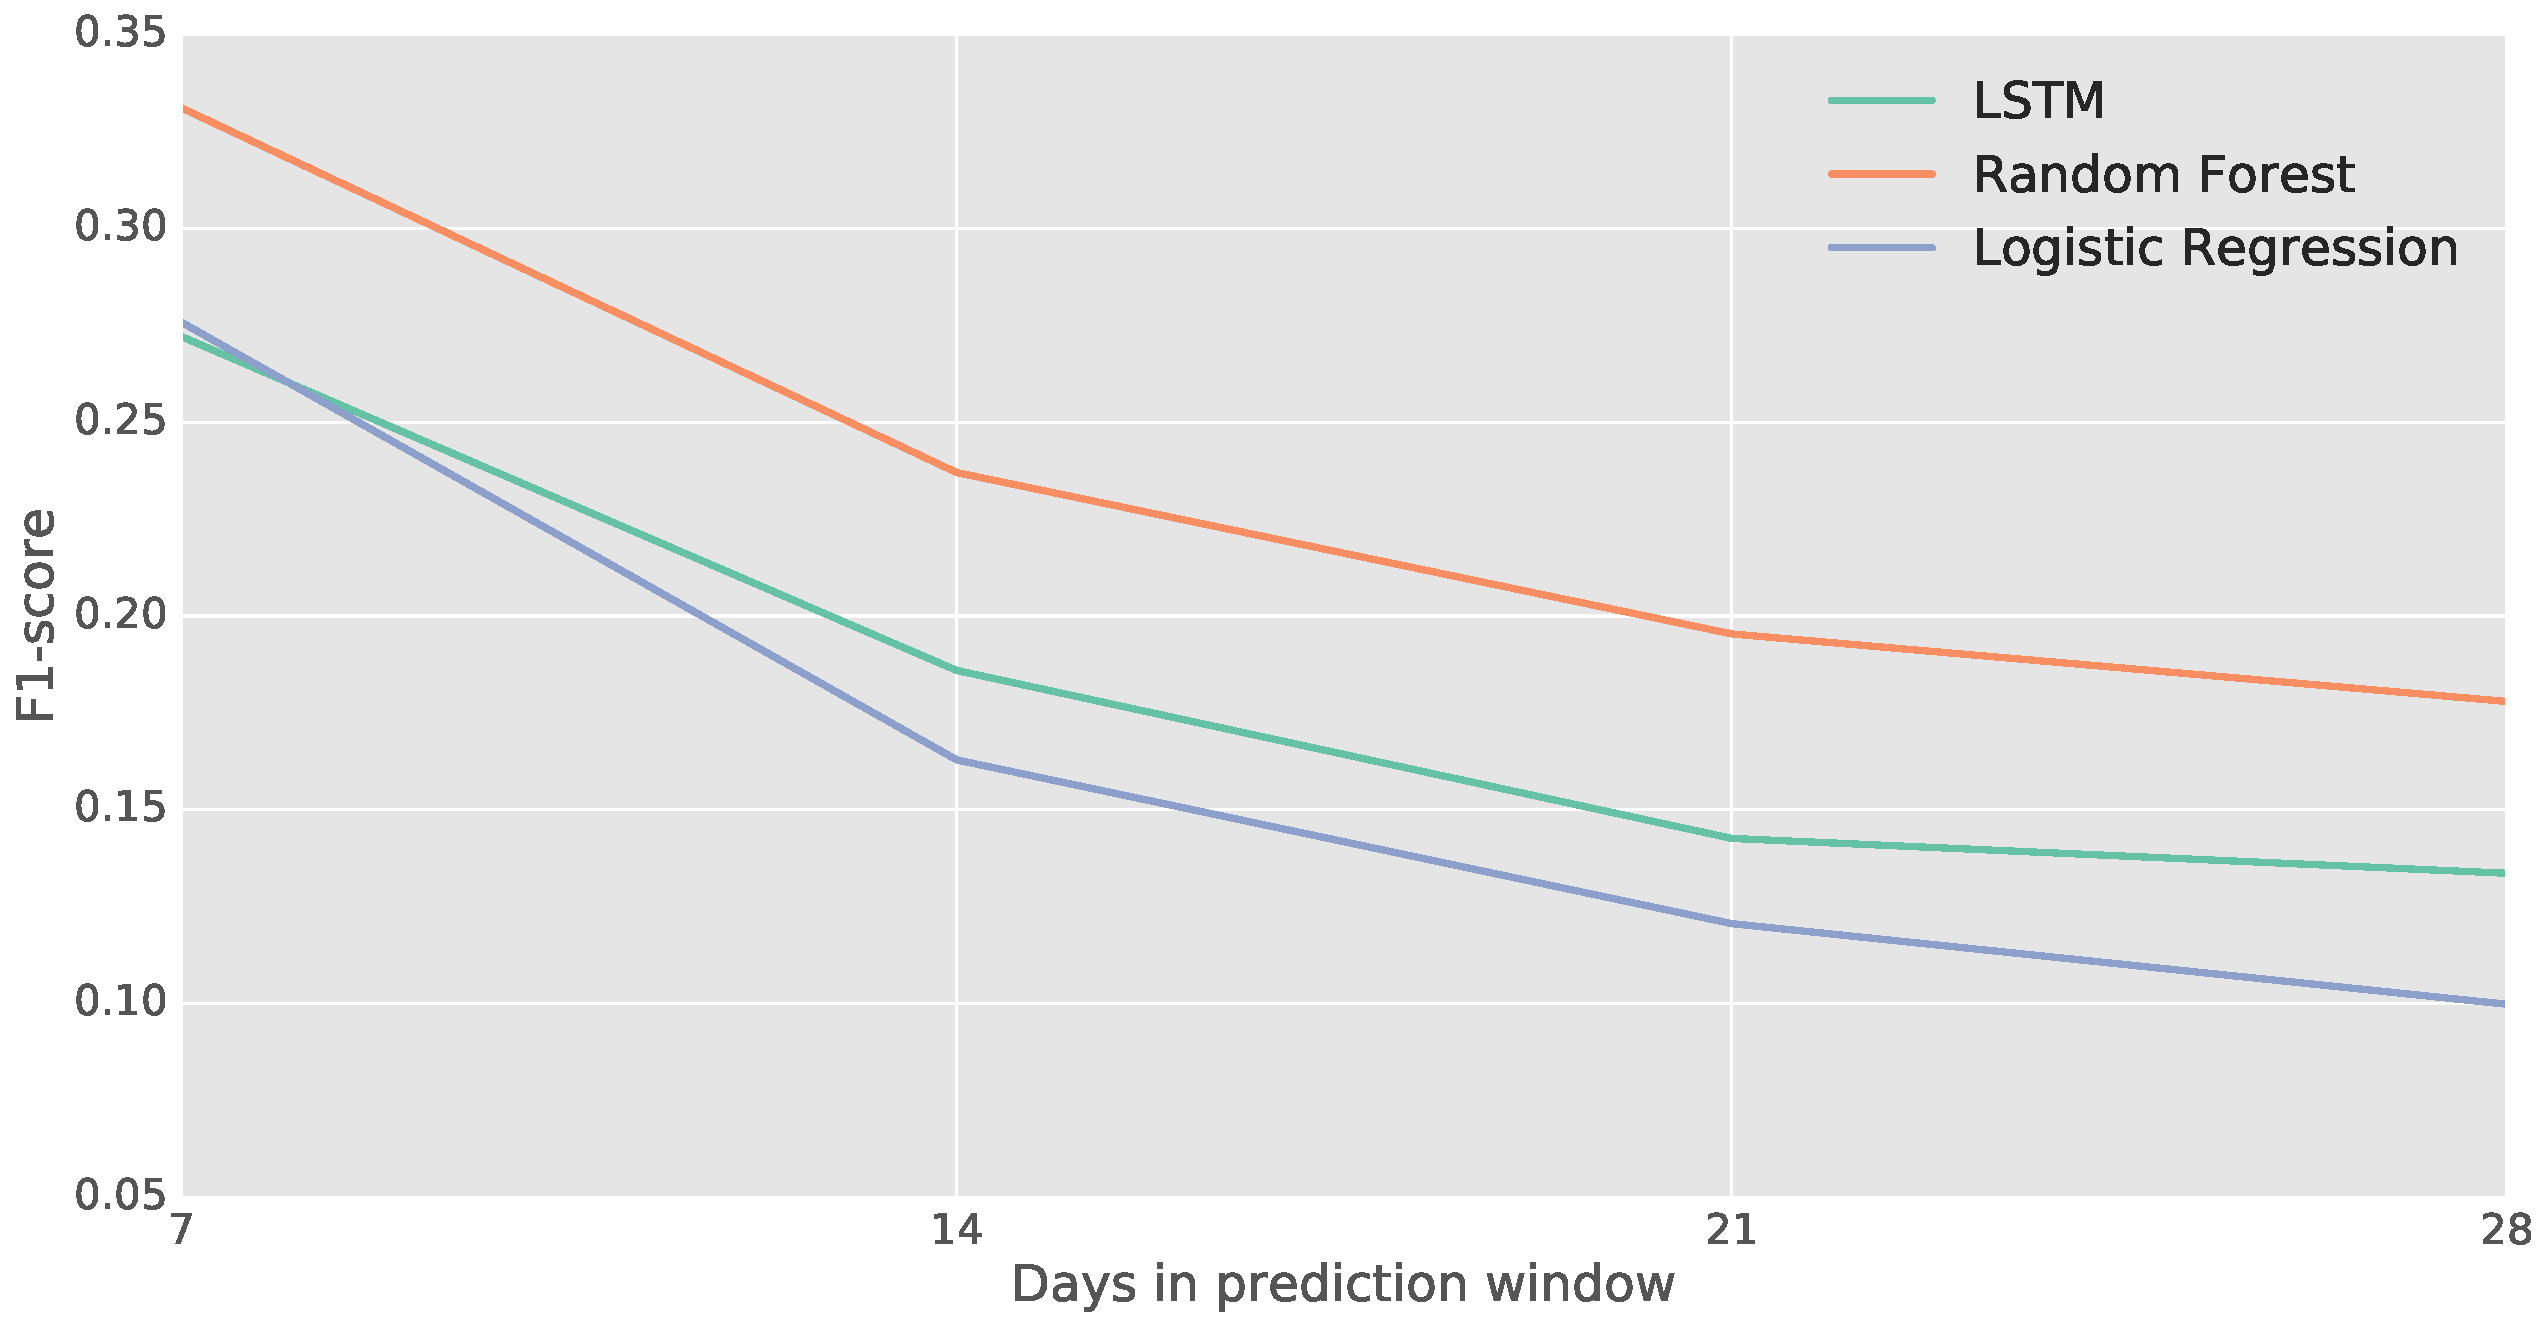
\includegraphics[width=1.0\textwidth,keepaspectratio]{figures/line_pred_window.pdf}
    \caption{F1-scores for the churned class for different prediction window sizes and models}
    \label{fig:line_pred_window}
\end{figure}

The same can not be said about the performance of predictor for the retaining class of \Cref{fig:line_pred_window_ret}. There is a gradual increase of the F1-score as more days are added to the window, however the difference only reflects the changes made in the  distribution of the retaining class. Precision-recall curves, ROC curves and a metrics table for this experiment can be seen in \Cref{fig:prc_pred_window}, \Cref{fig:roc_pred_window} and \Cref{tab:pred_window}, respectively.

\begin{figure}[H]
    \centering
    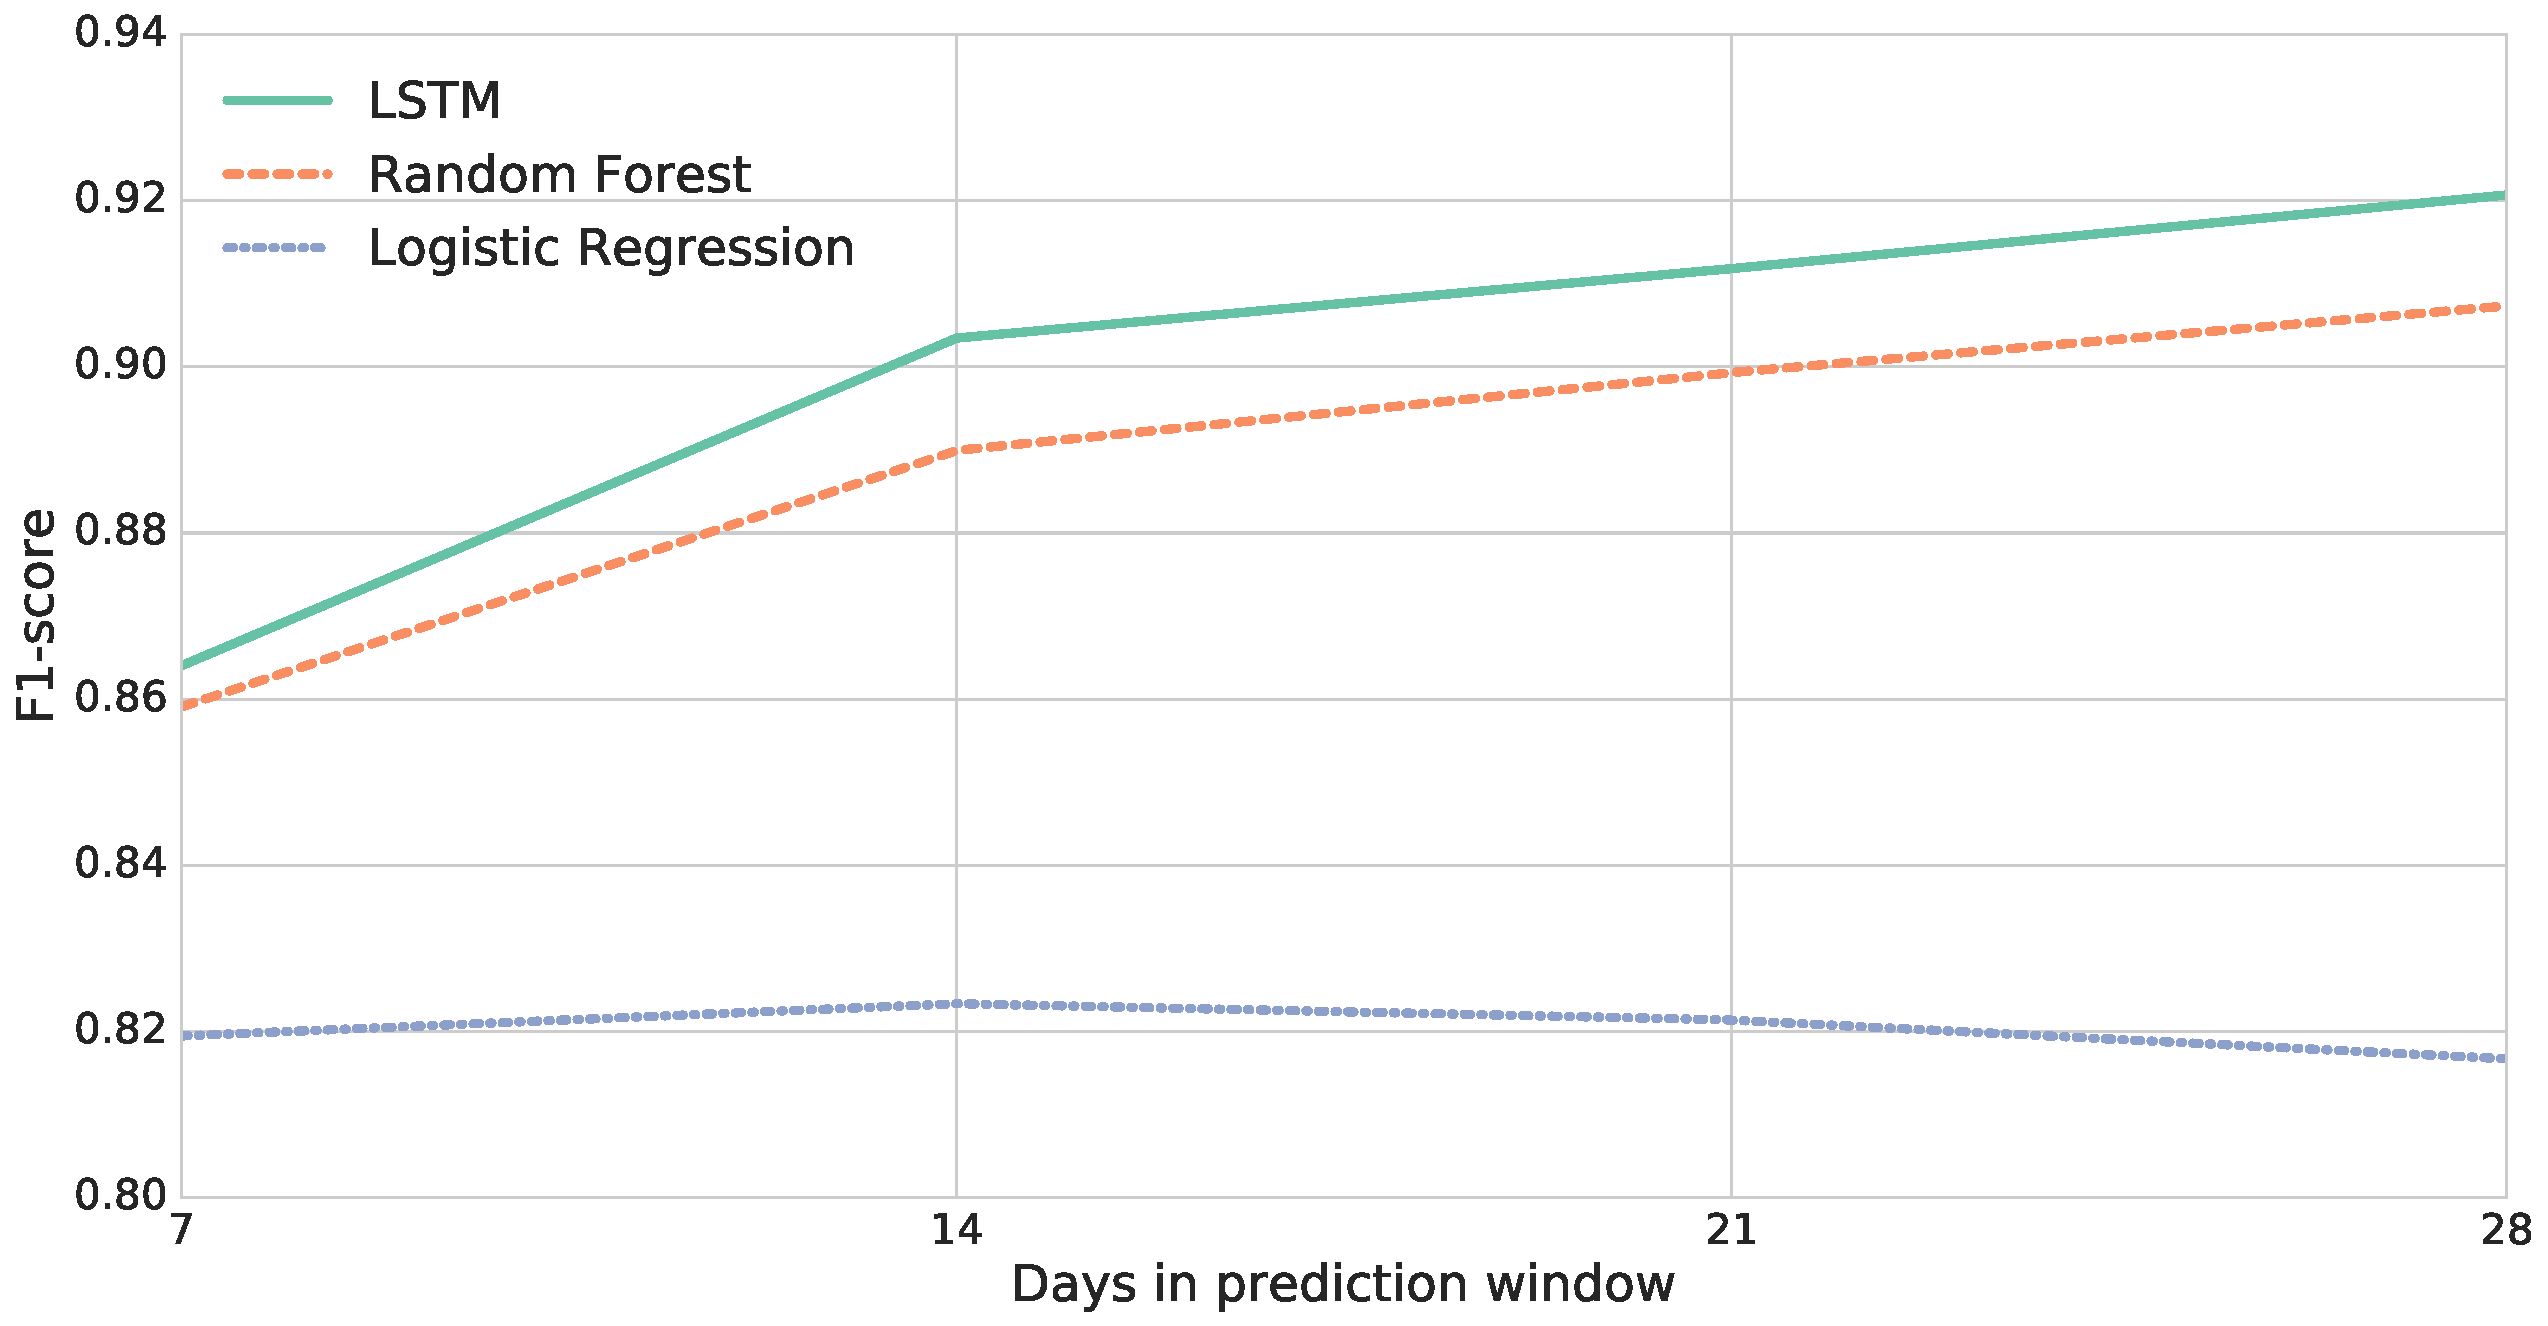
\includegraphics[width=1.0\textwidth,keepaspectratio]{figures/line_pred_window_retained.pdf}
    \caption{F1-scores for the retained class for different prediction window sizes and models}
    \label{fig:line_pred_window_ret}
\end{figure}

\section{Effect of Class Distribution}
\label{sec:exp_class_dist}

The distribution of the classes in the initial available dataset in this study is heavily skewed towards the retaining class. Training models with the data in this imbalanced state may yield an estimator that fails to capture the latent information of user behavior for the minority class, which is the one the service provider is commonly more interested in. There is often a gain in performance when narrowing the gap between the distributions of the retaining and churning labels \cite{Burez2009}. 

In this evaluation, we assess the performance of the models in terms of both precision and recall given different class distributions in the training data, while keeping the test data with its original skewed distribution. The ratio of churners is initially set to 10\%, with the remaining 90\% corresponding to the retained users. This difference is then gradually reduced until both classes have the same number of samples. We focus on the LSTM and random forest models, since logistic regression underperformed significantly in the previous experiments.

The resulting F1-scores of this experiment for both the churning and retaining classes can be seen in \Cref{fig:line_class_balance} and \Cref{fig:line_class_balance_ret}, respectively. The best performing model was obtained when the training data was closest to the real distribution between the classes, gradually decreasing its performance when the gap is reduced. The relative increase of F1-score between the top configuration and an equally balanced training data is of approximately $68\%$ for the LSTM model and $85\%$ for random forests. The performance of models when considering the retained class also improves in a similar fashion, however with a different magnitude: an increase of approximately $7\%$ for LSTM and $9\%$ for random forest can be observed between the top and the worst scoring configurations.

\begin{figure}[H]
    \centering
    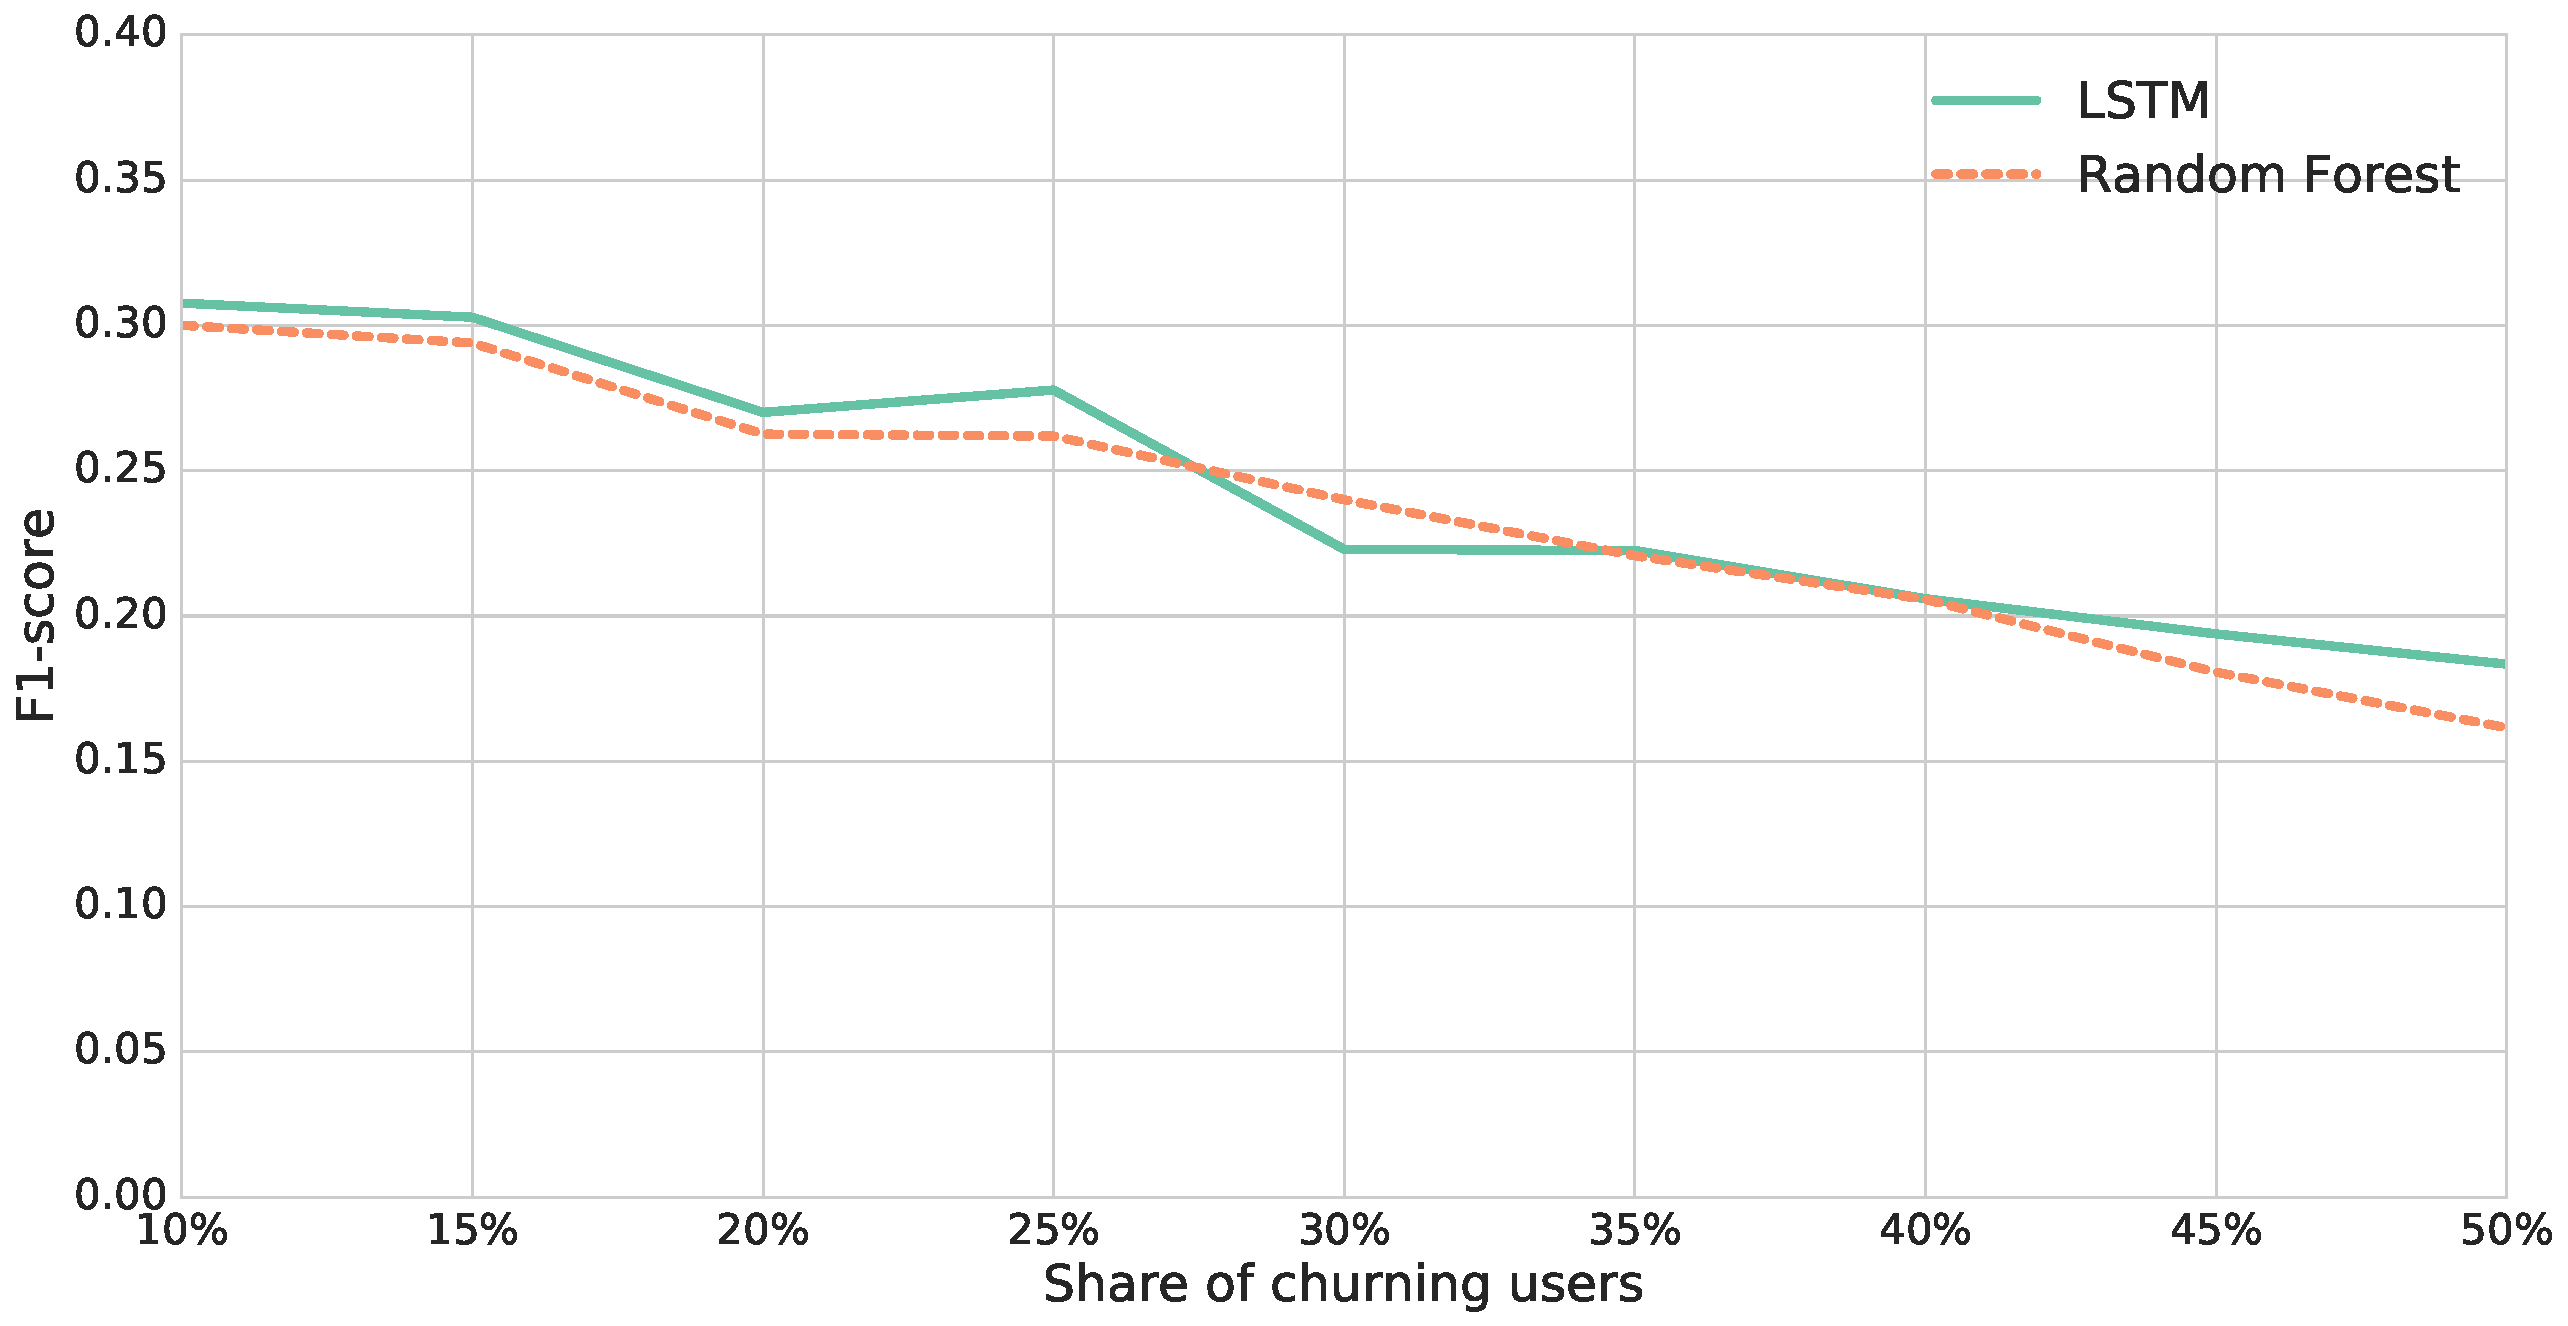
\includegraphics[width=1.0\textwidth,keepaspectratio]{figures/line_class_balance.pdf}
    \caption{F1-scores of the churning class for different class distributions.}
    \label{fig:line_class_balance}
\end{figure}

\begin{figure}[H]
    \centering
    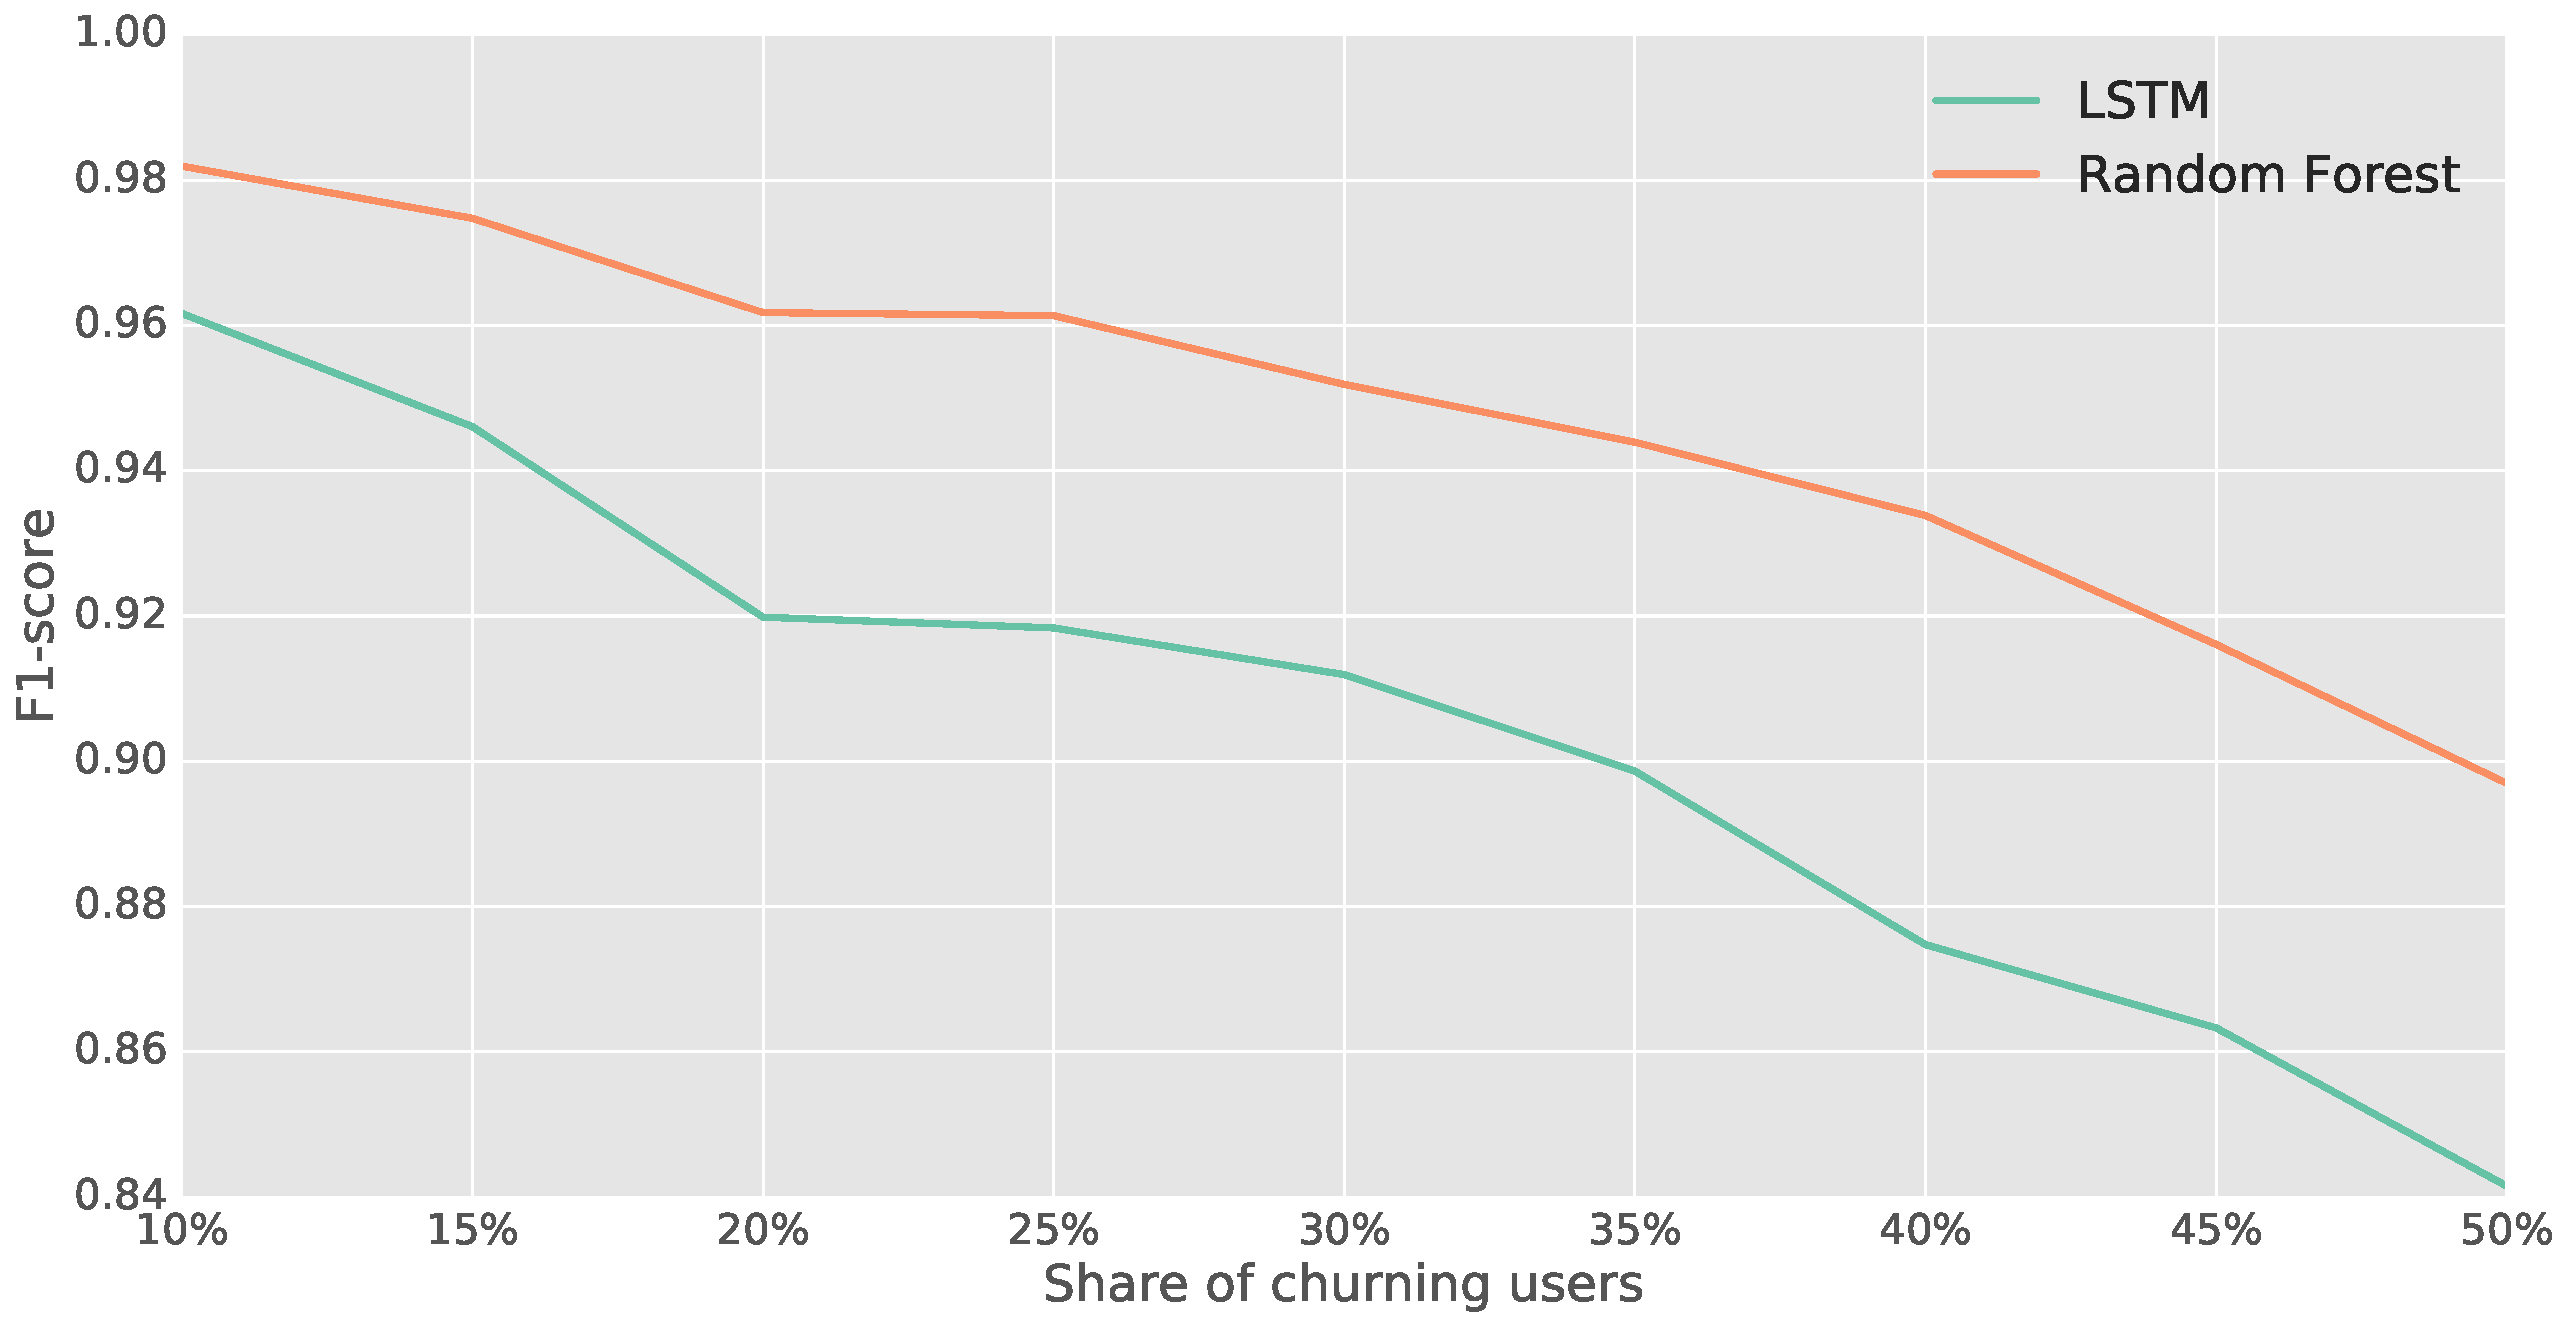
\includegraphics[width=1.0\textwidth,keepaspectratio]{figures/line_class_balance_retained.pdf}
    \caption{F1-scores of the retained class for different class distributions.}
    \label{fig:line_class_balance_ret}
\end{figure}

In \Cref{fig:prl_class_balance} and \Cref{fig:prl_class_balance_ret} it can be further inspected why the F1-score reduces as we narrow the distance between the class labels. As the rate of churning users of the training data increases, the gap between precision and recall metrics increases greatly. Higher precision is obtained when the distribution is closest to the one in the test data, while recall peaks both classes have equal number of training samples.

\begin{figure}[H]
    \centering
    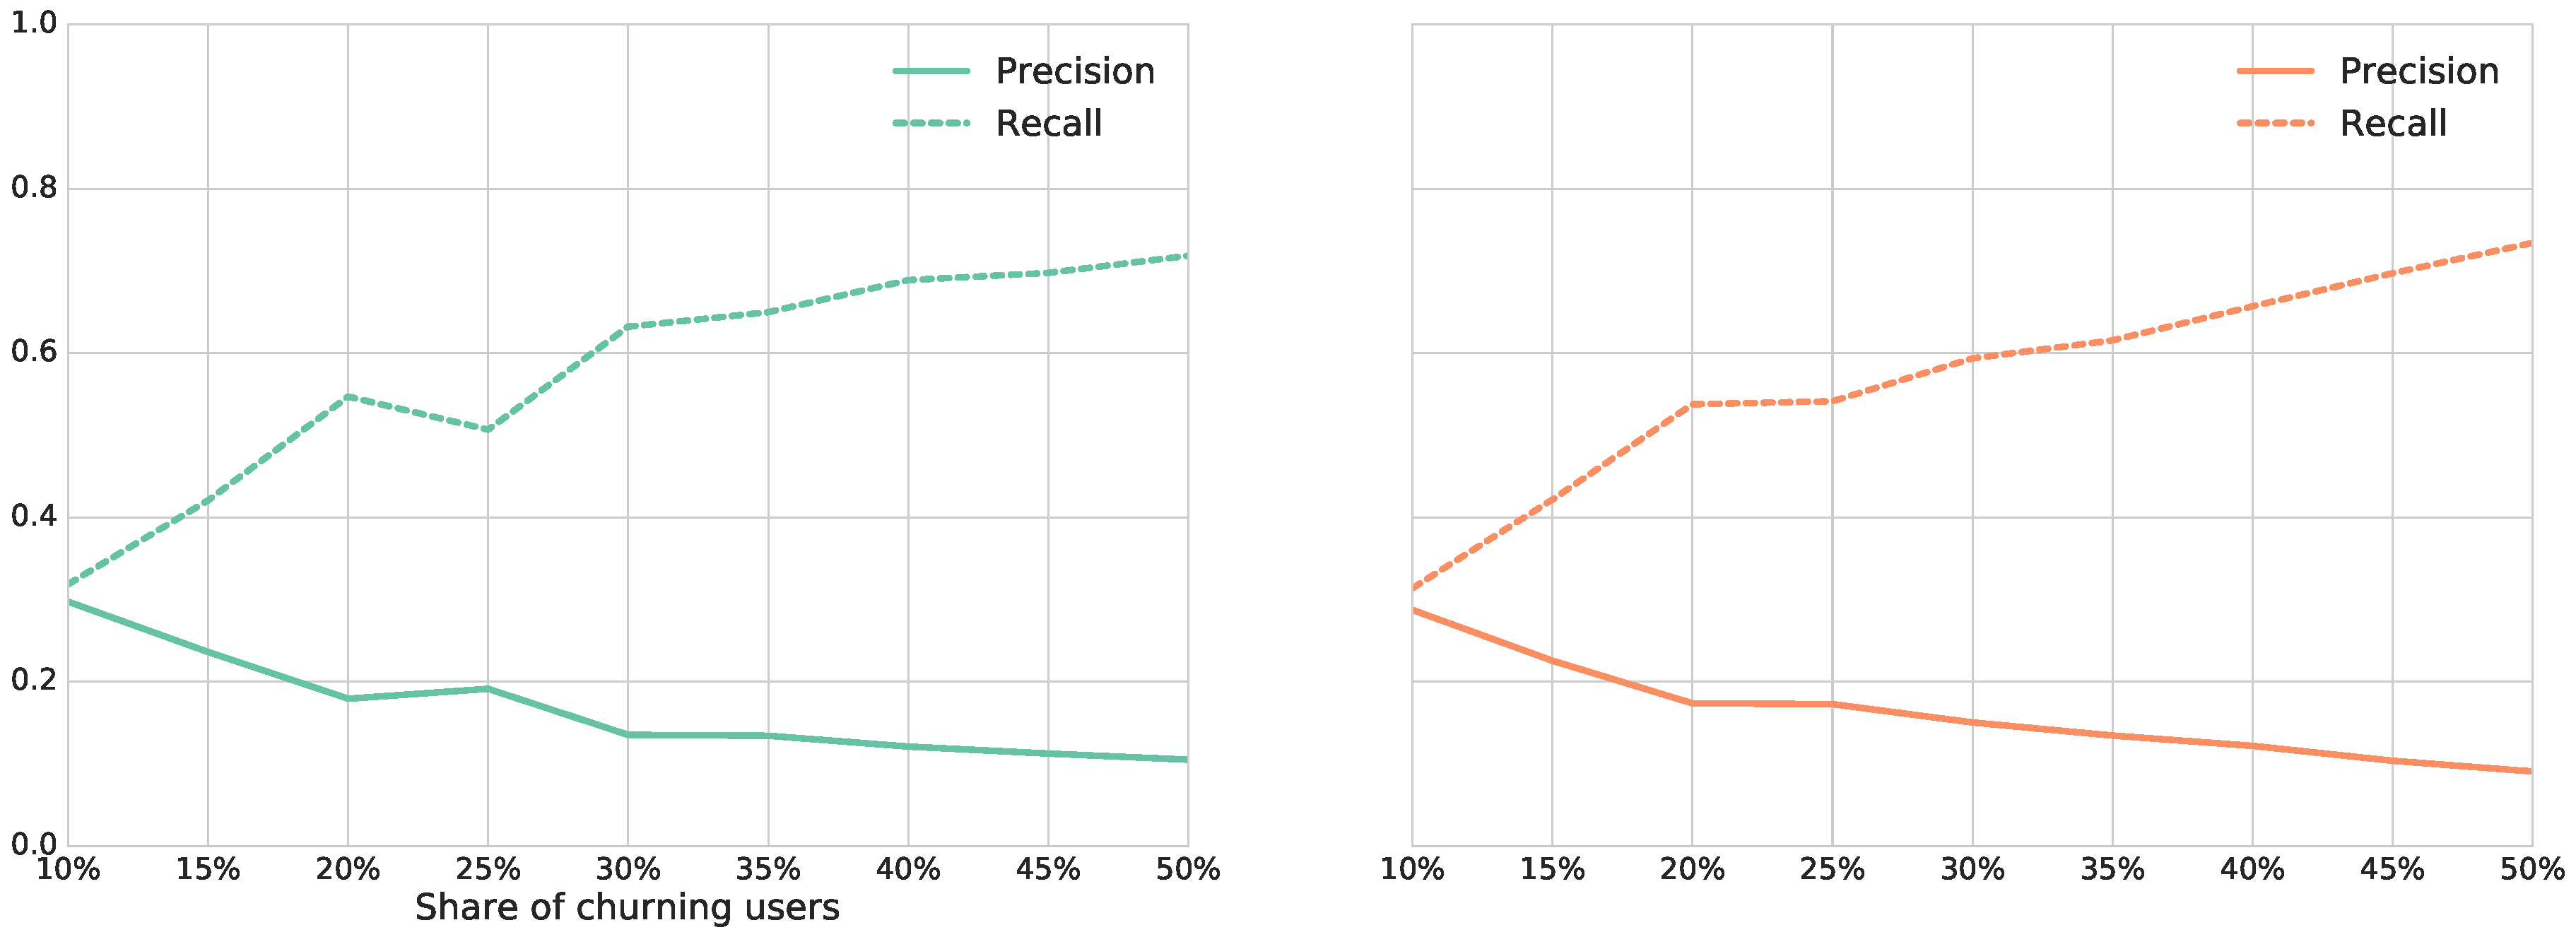
\includegraphics[width=1.0\textwidth,keepaspectratio]{figures/prl_class_balance.pdf}
    \caption{Precision and recall scores of the churning class for LSTM (left) and random forest (right) models.}
    \label{fig:prl_class_balance}
\end{figure}

\begin{figure}[H]
    \centering
    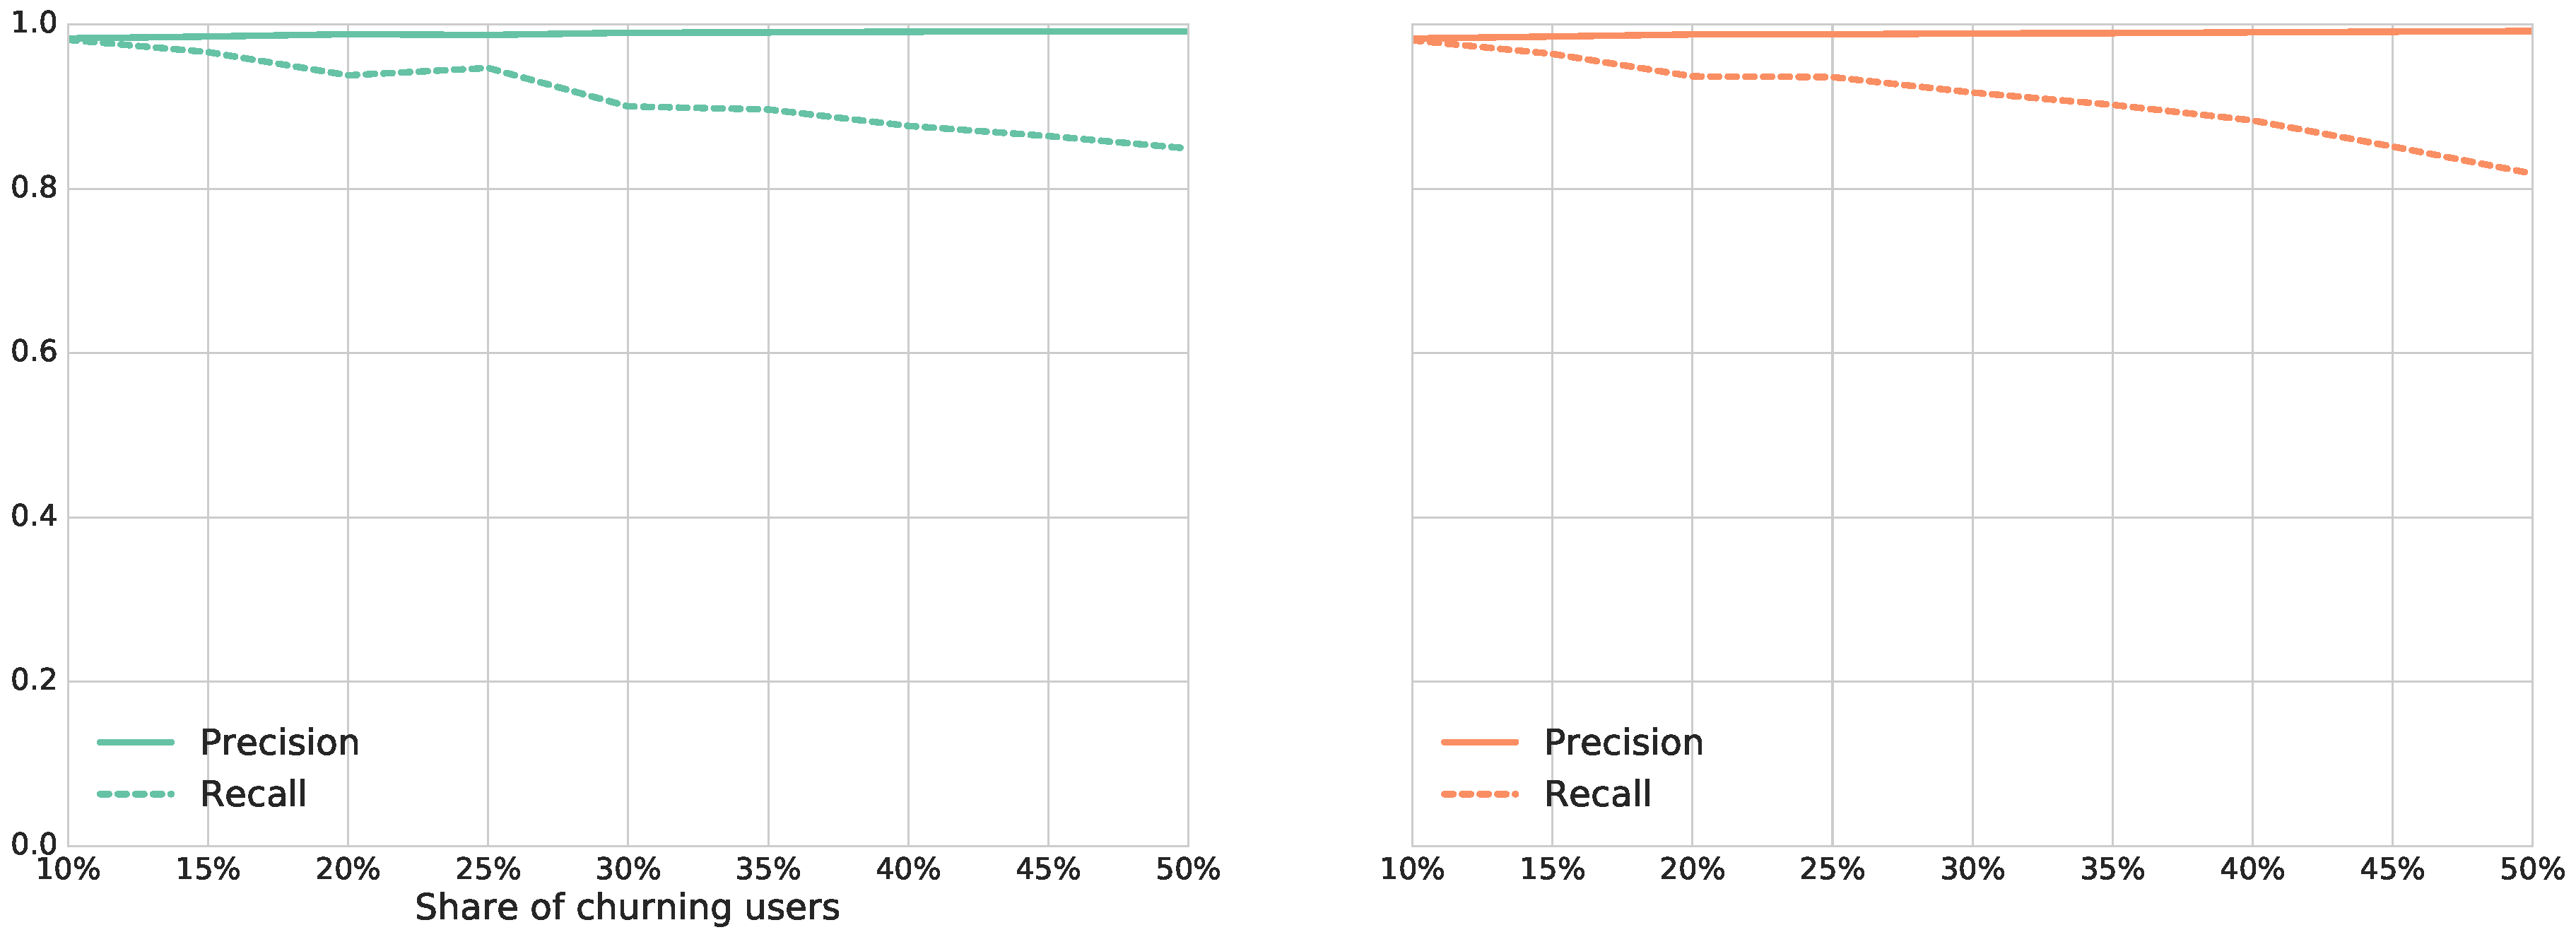
\includegraphics[width=1.0\textwidth,keepaspectratio]{figures/prl_class_balance_retained.pdf}
    \caption{Precision and recall scores of the retained class for LSTM (left) and random forest (right) models.}
    \label{fig:prl_class_balance_ret}
\end{figure}

\section{Experimenting with Dimensionality Reduction}

Given the data available, we created 52 features capturing user behavior through time. It is intuitive to think that not all of these attributes will have the same importance when predicting if the user is going to churn or not, some of them are highly correlated to each other as can be seen in \Cref{fig:correlation}. Having an excessive number of features may also lead to phenomenon known as "curse of dimensionality", where predictive models that learn through similarity of samples (implicitly or explicitly) may fail to achieve a good performance because examples are further apart from each other as more dimensions are used for representing the data \citep{domingos2012few}. 

Often the samples can be explained with some controlled loss of information by using a lower dimensional representation of the data. A common dimensionality reduction technique used for compression and visualization that attempts to maximize the variance of the dataset is PCA. In this experiment, we investigate the impact of applying PCA on the performance of the predictive model. We gradually increase the number of principal components the data is reduced to; starting from 4 components up to 52 which is the actual size of the features used without dimensionality reduction. We examine only the two best performing methods, that is LSTM and random forest.

The results of this experiment are shown in \Cref{fig:line_dim_reduction}. Here it can be seen that by selecting 16 principal components after reducing the data through PCA achieves highest F1-scores for both retaining and churning classes in the LSTM model, with a relative increase of approximately $18\%$ of the metric between the highest and worst scoring configurations for the churned class. The random forest model exhibits a more modest improvement when 28 principal components are selected, which configures a relative increase of $6\%$ in F1-score when compared to the uncompressed configuration of 52 features.

\begin{figure}[H]
    \centering
    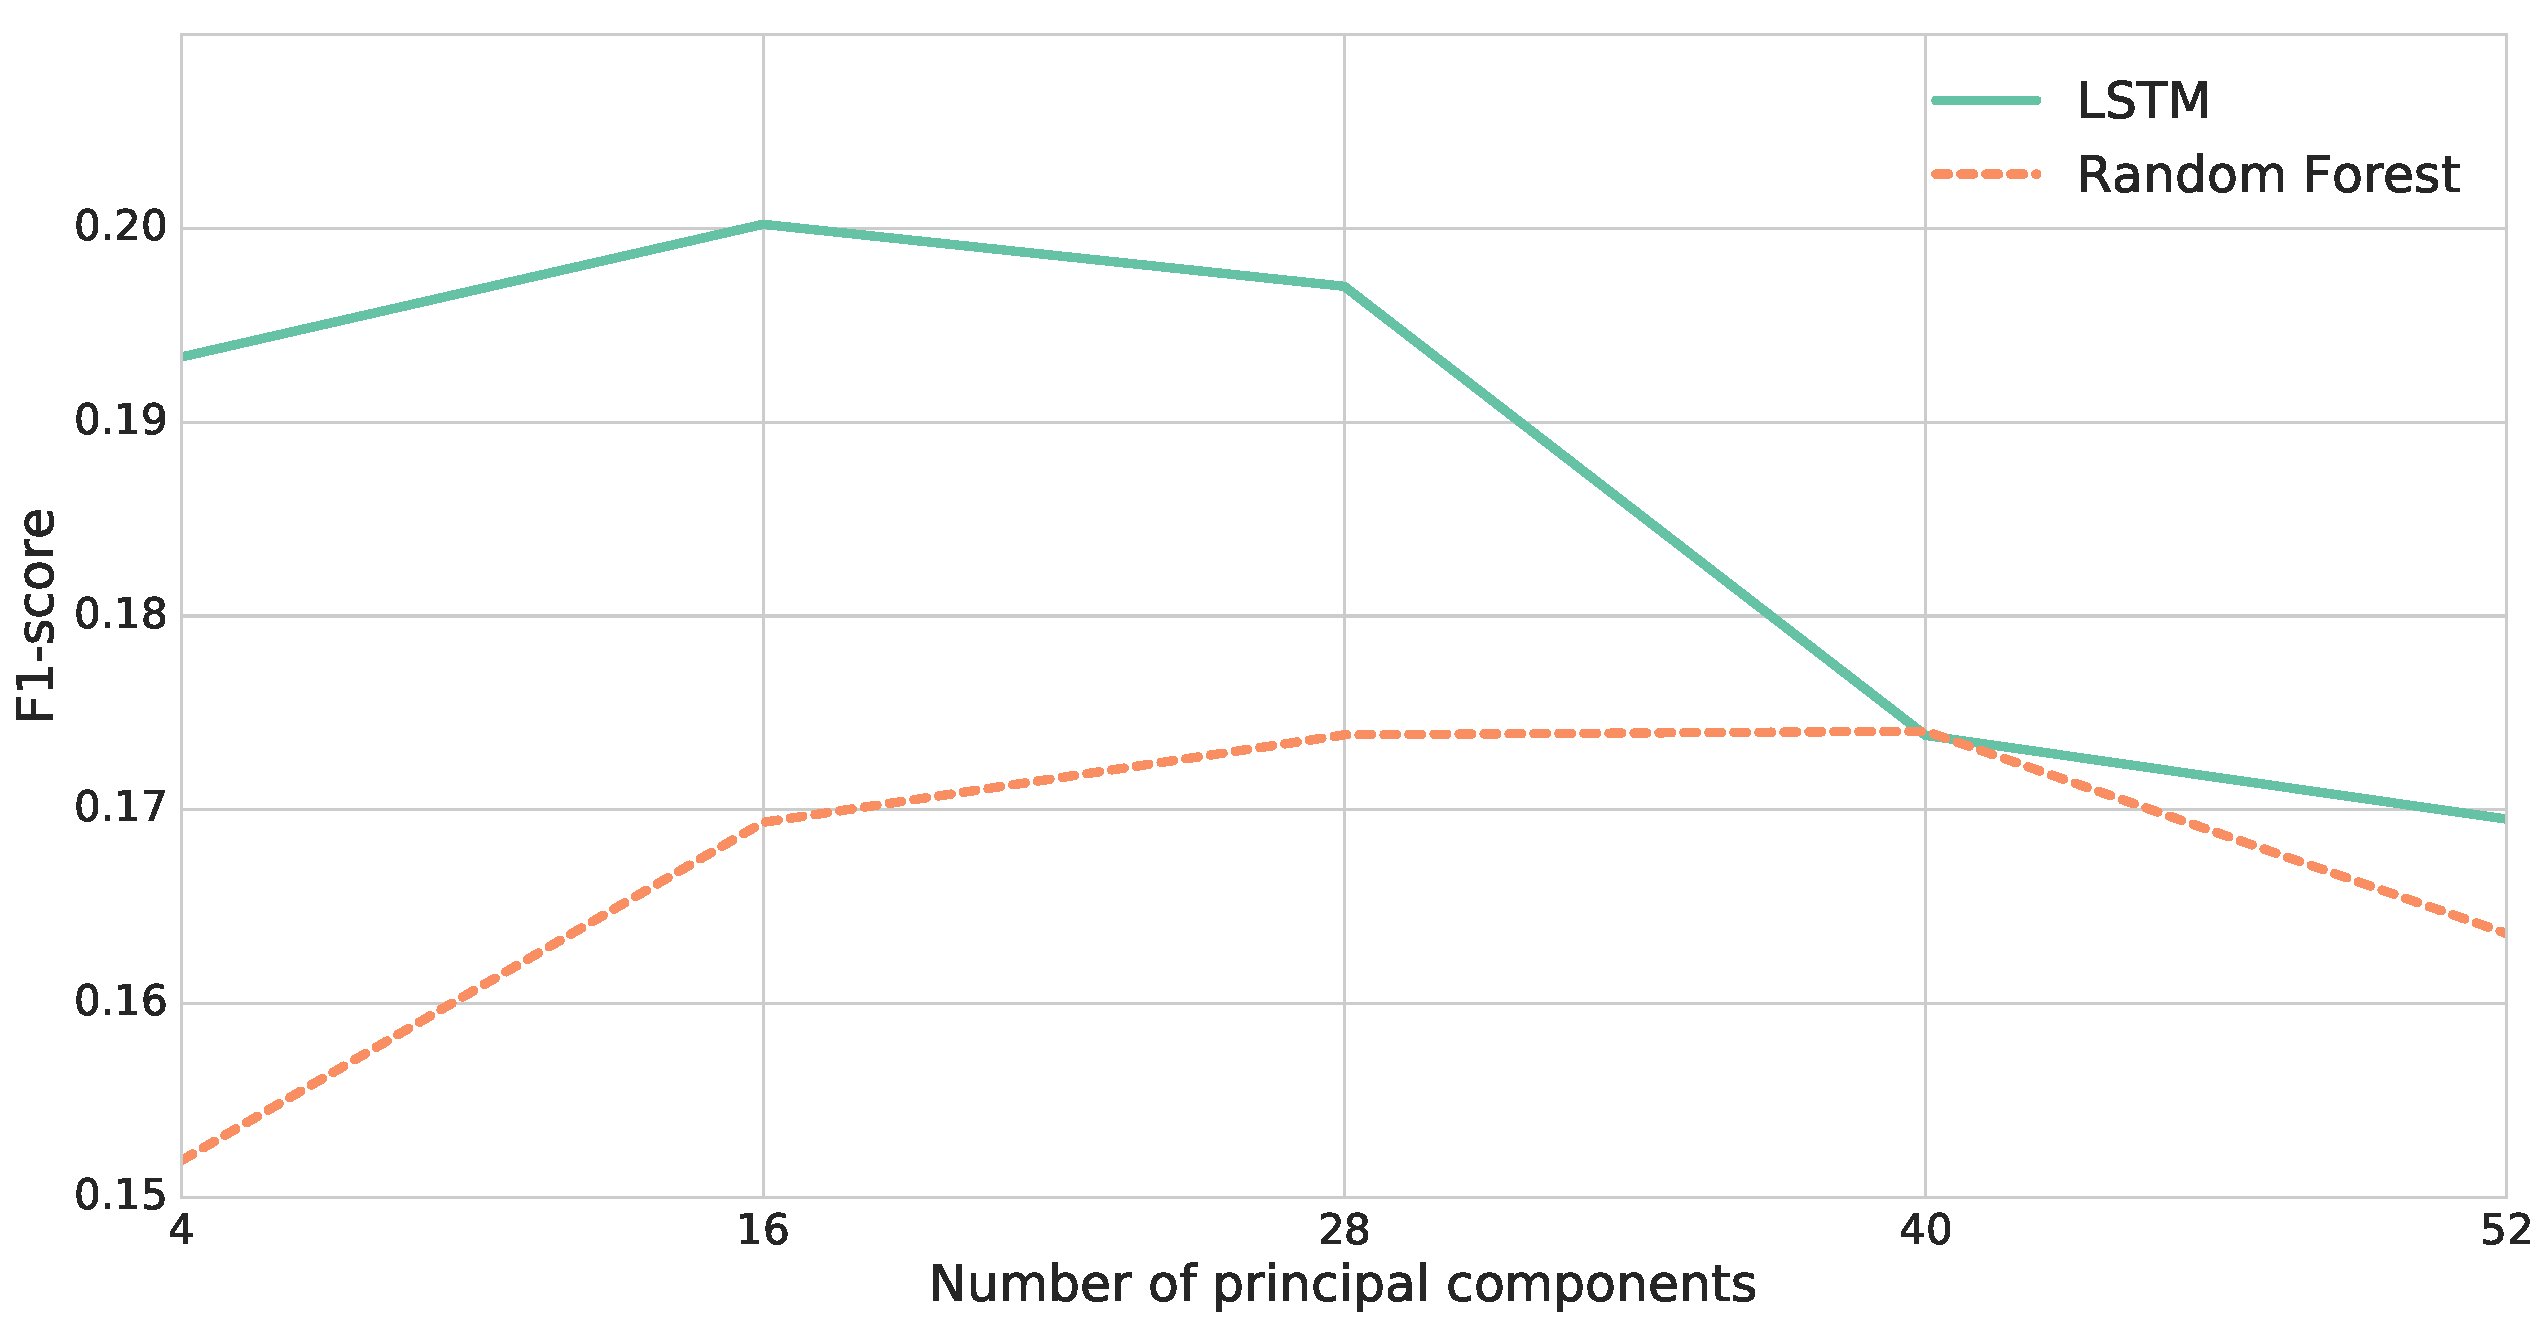
\includegraphics[width=1.0\textwidth,keepaspectratio]{figures/line_dim_reduction.pdf}
    \caption{F1-scores of the churning class for different number of principal components}
    \label{fig:line_dim_reduction}
\end{figure}

The retained class also shows an increase in performance when PCA is applied to the data, which can be seen in \Cref{fig:line_dim_reduction_ret}. However the performance gain is not as significant: a relative $3\%$ increase was observed for the LSTM model when comparing the top scoring configuration of 16 principal components and the uncompressed data, and of $1\%$ when selecting 28 principal components of the random forest model.  


\begin{figure}[H]
    \centering
    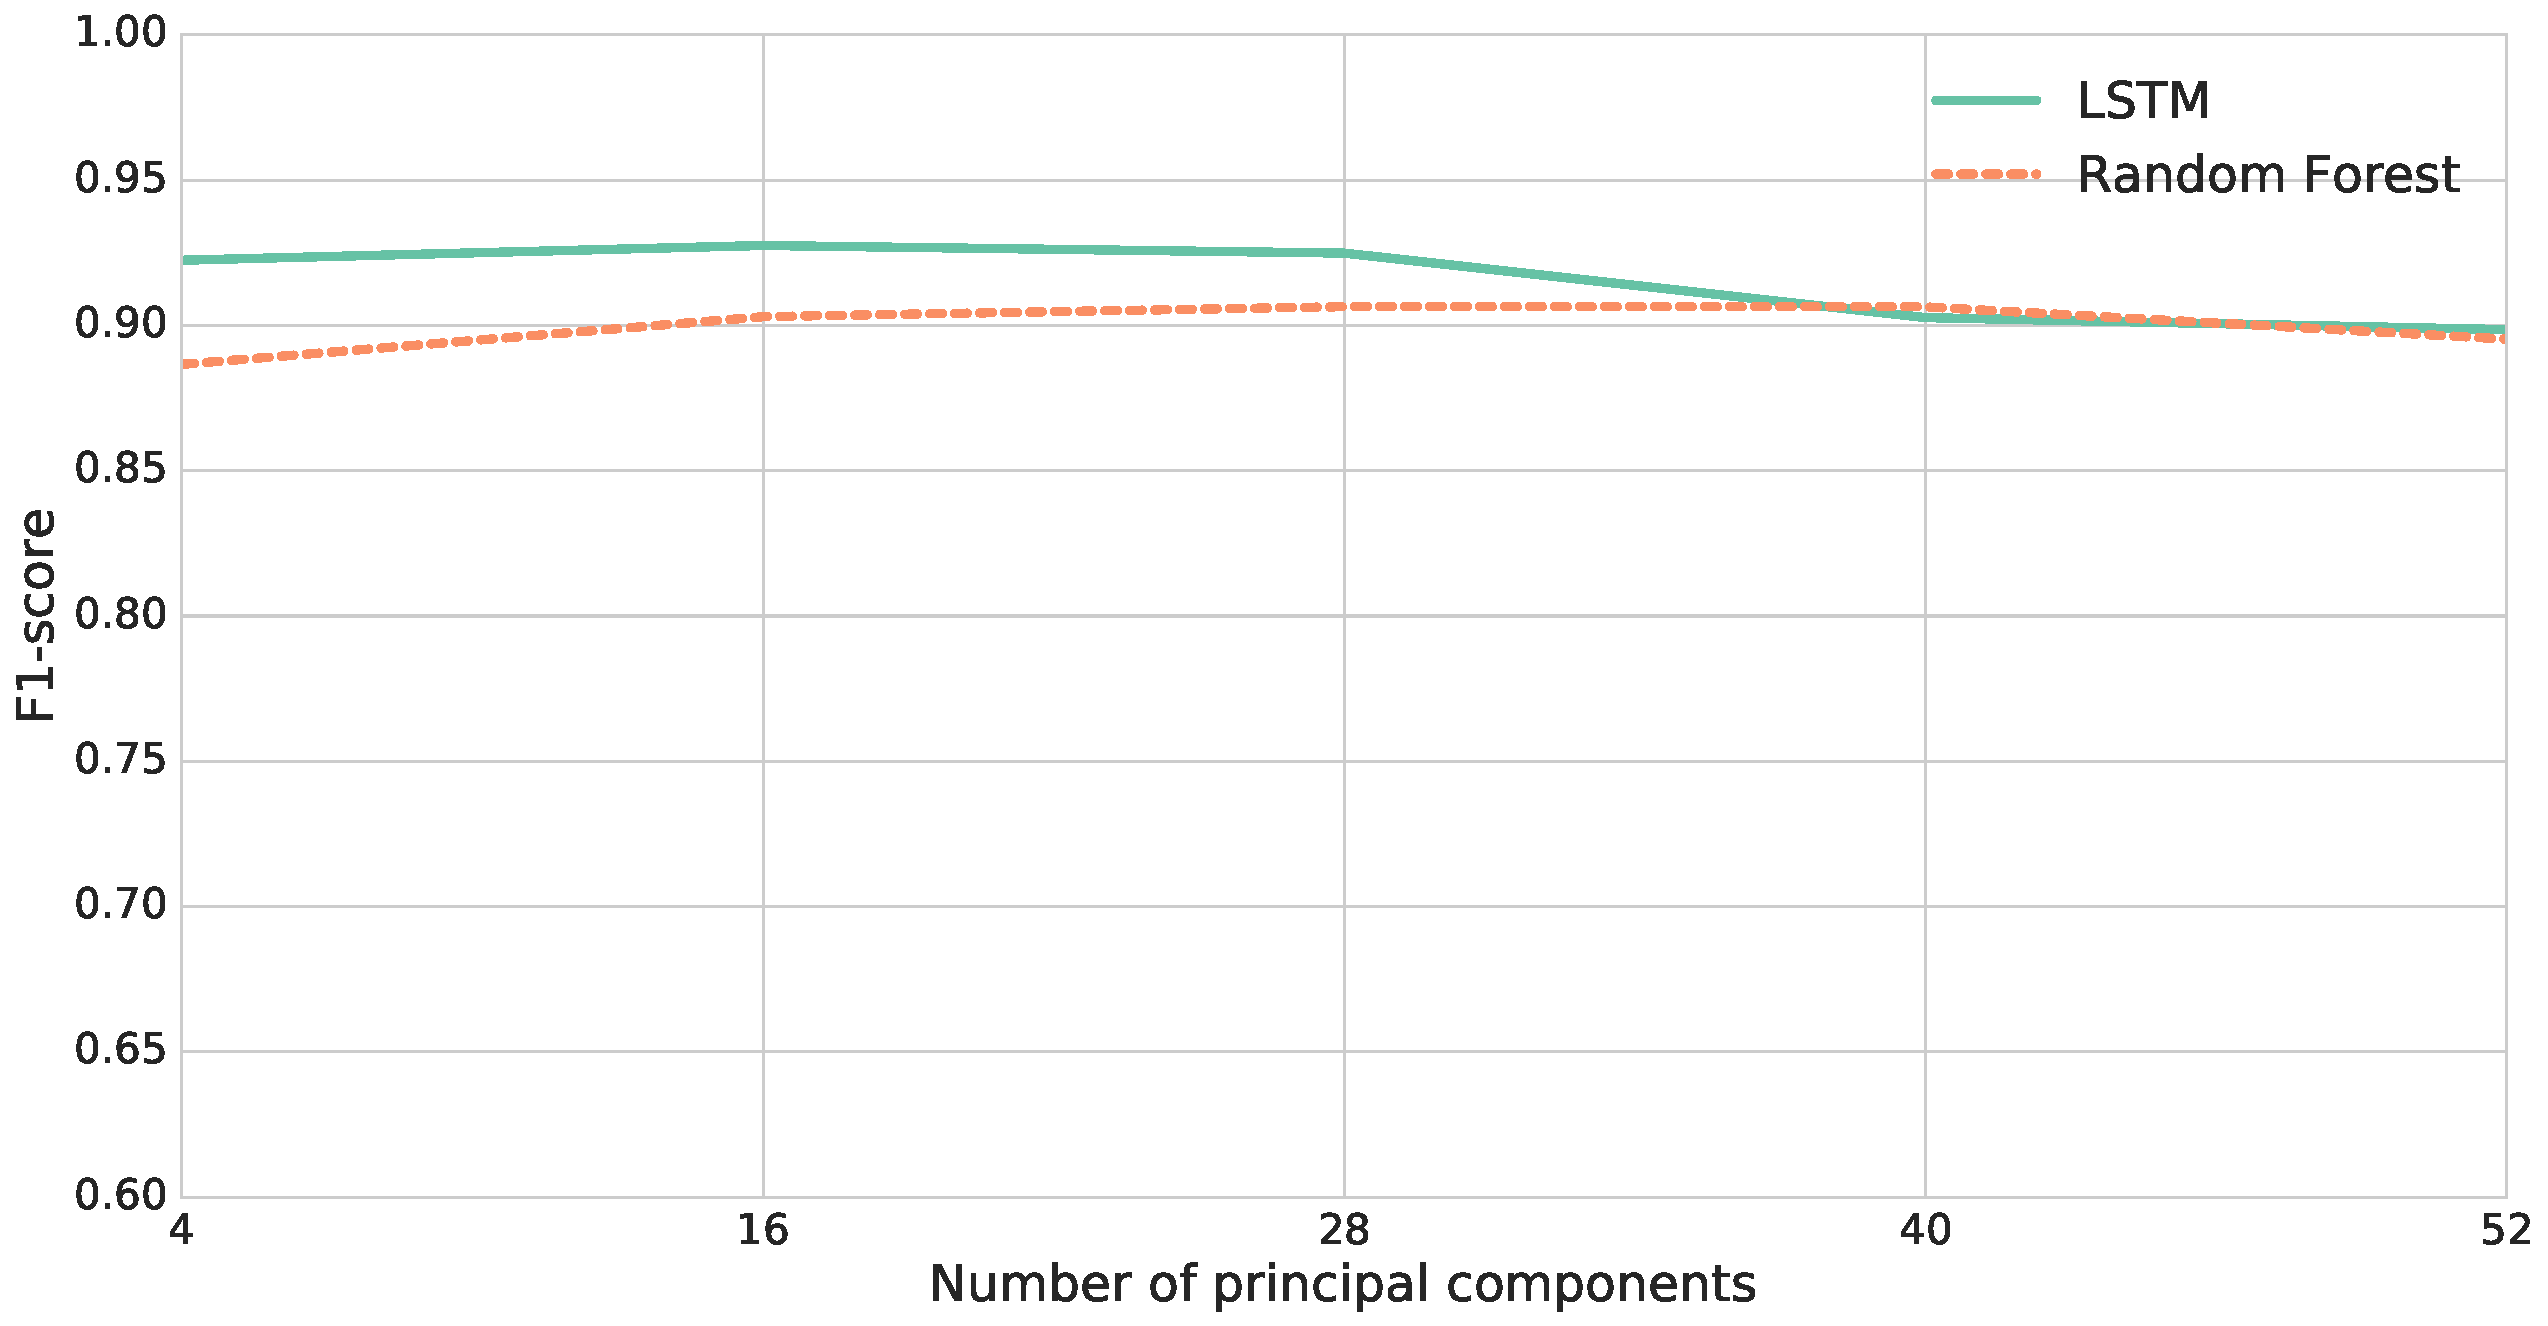
\includegraphics[width=1.0\textwidth,keepaspectratio]{figures/line_dim_reduction_retained.pdf}
    \caption{F1-scores of the retained class for different number of principal components}
    \label{fig:line_dim_reduction_ret}
\end{figure}


\chapter{Discussion}
\label{cha:discussion}

\section{Comparing LSTM to Baseline Models}
\label{sec:dis_lstm_baseline}

The experiments performed in this project showed that LSTM has a comparable performance to random forest for predicting user churn. Even though the evaluation metrics show a slight advantage to LSTMs, the difference is not enough to be considered conclusive as it can be caused by random noise in the data. The main metric chosen for evaluation, the F-1 score, had a top scoring result for every LSTM model in all experiments. The result was different when taking into consideration the area under the precision-recall curve, however: random forest has a small advantage in number of experiments for the PR AUC metric, which indicates that it outputs more confident probability estimates than LSTM, but the difference in this metric is minimal. 

It is clear from the results that logistic regression is not a suitable model for detecting user churn. Its performance is consistently underwhelming in all experiments that were performed.

Three reasons are hypothesized as to why similar results between LSTM and random forest were observed. First, decision trees (and consequently random forests) thrives when features in the dataset are good proxies for the identifying the latent variable being sought. Our dataset consists of 52 attributes that describes the customer usage over several different features of the service, attributes which allows the random forest models to learn the correlations between the input data and the churn labels with a reasonable accuracy. This feature engineering however does not come for free: it requires an extensive amount of insights from data experts that not only are difficult to conceive but also may fail to be valid for future versions of the service .

Second, the amount of temporal data fed to the LSTM models may have been insufficient for it to properly learn user behavior that can be linked to churn. The longest time period used for training was 56 days split into intervals of 8 hours, however customers commonly exhibits a seasonal behavior that this time range may fail to capture. \Cref{sec:exp_obs_window} shows an increase in the ability of the LSTM model to detect churn when historical data is added to training, which is an indicator that more data may be needed. There is a tradeoff however regarding the resources required to train the model: more data also means that more time and computing power will be needed to fit an LSTM estimator.

Finally, the goal of finding scores that are as unbiased as possible through the nested cross-validation technique ended up limiting the range of hyperparameters that could be explored with the LSTM. Neural networks are notorious for being costly to train, and fitting it to every data fold and choice of parameter proved to be prohibitively expensive even with all the computing resources at our disposal. This resulted in we only being able to sample a small set of random parameters for the LSTM, possibly not enough to compete with a full grid search used for the baselines. To mitigate that, one could do a standard train/validation/test split and use a larger dataset for fitting and evaluating the models, relying on its size for the accuracy of our metrics. If obtaining trustworthy scores is of more importance however, the nested cross-validation could still be performed by manually splitting the folds so the models could be trained in parallel, but that would require considerable amount of engineering work.


\section{The Class Imbalance Problem}
\label{sec:dis_class_dist}

One of the largest challenges of this project was the difficulties that training models with a heavily skewed dataset turned out to be. Our class of interest, the users that are going to churn in the future, represents only a small fraction of the sampled data, largely overwhelmed by the majority retaining class. While this is a positive indicator of business health, it proves to be problematic when the goal is to learn the patterns that represent good signals of a user leaning towards leaving the service in the future or not. This also raises questions regarding how a production-level system that predicts user churn could be implemented in a company, since by performing good predictions (allied with retention actions) the model will gradually lose performance as time goes by.

The results of the experiment on class distribution reveals that recall is at its peak when both retained and churned classes have the same number of training samples. This is due to the fact that undersampling has the underlying effect of setting the classification boundary to halfway between both classes, instead of being pushed towards the majority classes when data is in its raw state. On the other hand, precision is reduced since less data is used for training. The exact opposite, higher precision and lower recall, can be observed when the gap between the classes is wider.

When analyzing the results for the retained class, the precision marginally increases when the difference between the class labels is reduced. The recall however suffer a significant decrease, which can be attributed to the reduced number of retained samples removed through undersampling of the training set.

The effect of this imbalance between classes can clearly be seen in the precision metric of all experiments. Even if only a small fraction of the retaining class is misclassified, the sheer number of negative samples overwhelms the amount of true positives, driving the precision score quickly down. When taking into consideration both precision and recall, the experiment that proved more fruitful was changing the size of the prediction window, where the top scoring F1-score and PR AUC was obtained when the window was smallest in size. 

The number of samples of the churning class plays an important role on the performance of the predictive models. Having only a small fraction of user samples that are abandoning the service in the future may be insufficient for the estimators to learn the patterns that correlates to churn. The random undersampling technique modifies this distribution as to artificially increase the importance of the churning samples, however several data points that could be used for training are lost in this process. 

Three approaches could be implemented as to mitigate this problem. First and foremost, more data could be used. The provider has no lack of user information stored in its databases, however this approach brings issues regarding the scalability of the solution that may be difficult to solve. Second, a smarter undersampling technique like Tomek links \citep{tomek1976two} or edited nearest neighbors \citep{smith2014instance} may present better results when compared to a simple random elimination of samples of the majority class. Third, the importance of the churned class could by means of a customized loss function that greatly penalizes when a retaining user is misclassified as a churner or by using a boosting algorithm like XGBoost \citep{chen2016xgboost} that automatically assigns a larger weights for the misclassified samples. The binary cross entropy loss function used for training the LSTM models in this project makes no distinction between the positive and negative classes, assigning an equal weight to both. Exploring different types of loss functions could yield better results to our models.

The choice of training models with a balanced distribution of classes is reasonable to a company when the expected cost of retention actions is low: it is safer to have false positive in the prediction of churn users than losing a customer. The choice for balanced is thus deemed suitable for the provider's objectives of minimizing churn. 

\section{The Impact of the Time Windows}
\label{sec:dis_time_windows}

We performed an experiment to assess the impact on the F1-score metric for predicting user churn when the size of the prediction window was tested with several different values. It was shown that the smaller the prediction window is, the higher the accuracy of the churning class in all of our predictive models, while increasing its size decreases the score gradually. It was also observed how the performance of the LSTM model increases when more historical data is available for training.

One of the reasons that may influence the observed results is that changing the prediction window length does have an underlying effect of modifying the distribution of the data by increasing the ratio of churners when the prediction window is smaller in size. The class balance experiment however contradicts the hypothesis that this is the reason for the observed performance gain, since the top F1-score was obtained with less churners in the dataset.

Another hypothesis is that the estimators can more precisely predict events in the near future when compared to forecasting the disposition of a user towards churning or retaining the application weeks after the last observed data point. It is intuitive to notice that our predictors encompass a degree of uncertainty that increases as the gap between the time of the last observed sample and the present date grows wider. Since by our definition the estimators output a single label at the end of the time windows, there is no natural way of encoding the confidence that the model has in its prediction at each point in the future time. This could be obtained however if the models experimented on can output a sequence with probability scores assigned to each time step, as can be achieved through a sequence-to-sequence LSTM \citep{cho2014learning} model or through survival analysis \citep{ibrahim2005bayesian}.

It must be stated that having a smaller prediction window means applying a more restrictive and aggressive definition for retention; a user has to be more frequently active in the product to be considered retained. However users may have a usage pattern that does not fit into the time window, thus switching between the churning and retaining classes more frequently as time goes by and yielding a churn label that could be considered less accurate by the service provider. The optimal size of this window is a parameter that must more importantly map to the goals that the service provider has with the predictive models, a intuitive value being one that express more precisely the business health metrics of the company.

\section{Training Time}

The performed experiments demonstrated that the LSTM achieves a reasonable performance when compared to the baseline models. However the difference between LSTM and the random forest model is marginal at best. One point to consider is the time that it takes for training both top scoring predictive models. Even though this was not a metric tracked in this project, it can easily be observed that random forests can be trained in a fraction of the time of even a shallow LSTM model. This can be a limiting inconvenience if the goal of the company is to set up a predictive model in production that is regularly updated with new user information. The small difference in accuracy may justify the choice for random forest in a situation where the service provider would rather train a model in hours and pay the difference in misclassification cost instead of waiting for the LSTM model to train for a small performance gain. 

\section{System Improvements}

This project was implemented as a proof of concept. We randomly undersampled the data such that it has a fair representative of the whole user base. The next step would be to scale up this work to production levels on the service provider infrastructure. 

The data pipeline was implemented using two technologies: Google's BigQuery and Apache's Spark, both highly scalable frameworks. On the other hand, the training of models was performed in a single powerful machine in the Google Cloud, where the data was loaded in memory before the cross-validation procedure, which is definitely a bottleneck of our system. Training the LSTM in batches on a single machine keeps the memory overload constant through time, but still doing a single training pass over all data points can be highly time consuming to compute, while also not making any use of the cluster of other machines that are at our disposal. 

A more promising alternative would be to implement the training process in a way that allows horizontally scaling the system by adding more and less powerful machines, instead of having a single one with expensive hardware. Downpour SGD is a method proposed by Dean \emph{et al.} \citep{dean2012large} as to distribute the the forward/backward pass and weight update of a neural network over a cluster of machines.

\section{Future Work}
\label{sec:future_work}

Another approach that could be beneficial for the task of predicting user churn is to consider the output of the models as sequences, assigning one label per user per time step in the observation period. This project assigned a single binary label for each user in the dataset by considering a unique time span in the future to judge whether a user is leaving the service or not. However this approach fails the capture the user that returns to the application after some small periods of absence, and also turning the task of predicting the behavior of users that stream content infrequently more challenging. By having a label for each time step in the observation window, the behavior of the user through time could be more precisely mapped, and the changes of disposition towards the application more easily visualized. Minor modification in the architecture of the LSTM can transform the output of the model into a sequence, however it would be necessary to choose another baseline for comparison that could extract the temporal information in a similar way. A classic hidden Markov model could be a suitable candidate for this task, for example. 

Going deeper into the method chosen for representing the customer labels, the task of prediction could be turned into a regression problem by trying to answer the question of \emph{when} a user is going to churn instead of \emph{if}. Users that are going to abandon the service would have a timestamp assigned instead of a binary positive label, which would specify the moment in time that the customer is churning. A good baseline with this approach would be survival analysis \citep{ibrahim2005bayesian}, a statistical method for analyzing the expected time that an event is happening and also its duration. Meanwhile retaining users could be assigned a threshold value far off in the future to indicate our uncertainty of the churn event. The works of Tax \emph{et al.} \citep{Tax2016} shows an impressive performance when predicting when an event of a business process is going to take effect by making use of an LSTM model, and the same methodology could be mapped to a service provider by predicting when a user is going to churn instead. 

The problem could even be made more general and predicting instead when the user is going to stream content in the platform, being the threshold value in the future an indication that the user has left the provider. Posing the problem in this way would also allow any other event in the platform to be tracked, like for example when a customer would make use of a specific feature of the application. 


\chapter{Conclusions}
\label{cha:conclusion}

The main topic of this thesis was predicting churn -- whether a customer is going to abandon a service provider. Well known classifiers like logistic regression and random forest were used as a baseline for comparison of a newer approach in the form of a recurrent neural network called LSTM. It has been shown that LSTM has the overall best F1-score metric over all experiments and models evaluated. Random forests has a small advantage in the precision-recall AUC over LSTM. The difference in the evaluated metrics between the two models are minimal however, thus random forests and LSTMs are concluded to be comparable algorithms for predicting churn. Logistic regression on the other hand demonstrated an underwhelming performance in all experiments, therefore being an unsuitable method for churn detection. 

The performed experiments explored the influence that different aspects of the data used for training had in the final accuracy of the predictive models. The maximum harmonic mean between precision and recall for the churning class was obtained when the time span used for predicting if the user retained or not was limited in 7 days in the future, gradually decreasing as this time window increases in size. The ratio between the class labels also had a significant impact on the F1-score metric, where the maximum value was obtained when the distribution of the training data over the retained and churned classes was closest to the real distribution of the test set, at the cost of a low recall. If service providers are more interested in capturing the majority of potential churners, a balanced dataset for training is the suggested approach.

Finally, a framework for creating a dataset suitable for training churn prediction models was given, alongside a basic exploration of its features which gives an overall picture of the behavior of the user cohort of the service provider. This could be further explored by the company as to develop retention actions that could reduce levels of churn and thereby increasing profit.  

\bibliography{references}

\appendix

\chapter{Additional Results}
\label{cha:add_results}

\section{Metrics tables}

% --------------------

\begin{table}[h]
\centering
\begin{tabular}{lllrrrr}
\toprule
     &   &          &  F1-Score &    PR AUC &  Precision &    Recall \\
Models & Days & Label &           &           &            &           \\
\midrule
\multirow{8}{*}{LSTM} & \multirow{2}{*}{7} & Retained &  0.864 &  0.985 &   0.980 &  0.773 \\
     &   & Churned &  \textbf{0.339} &  \textit{0.333} &   \textbf{0.215} &  \textbf{0.795} \\
\cline{2-7}
     & \multirow{2}{*}{14} & Retained &  0.903 &  0.992 &   0.988 &  0.832 \\
     &   & Churned &  0.256 &  0.255 &   0.154 &  0.758 \\
\cline{2-7}
     & \multirow{2}{*}{21} & Retained &  0.912 &  0.994 &   0.991 &  0.844 \\
     &   & Churned &  0.214 &  0.213 &   0.125 &  0.749 \\
\cline{2-7}
     & \multirow{2}{*}{28} & Retained &  \textbf{0.921} &  \textit{0.994} &   \textit{0.992} &  \textbf{0.858} \\
     &   & Churned &  0.196 &  0.180 &   0.113 &  0.727 \\
\cline{1-7}
\cline{2-7}
\multirow{8}{*}{Random Forest} & \multirow{2}{*}{7} & Retained &  0.859 &  0.984 &   0.979 &  0.765 \\
     &   & Churned &  \textit{0.331} &  \textbf{0.334} &   \textit{0.209} &  \textit{0.792} \\
\cline{2-7}
     & \multirow{2}{*}{14} & Retained &  0.890 &  0.991 &   0.989 &  0.809 \\
     &   & Churned &  0.237 &  0.259 &   0.140 &  0.770 \\
\cline{2-7}
     & \multirow{2}{*}{21} & Retained &  0.899 &  0.994 &   0.991 &  0.823 \\
     &   & Churned &  0.195 &  0.227 &   0.112 &  0.756 \\
\cline{2-7}
     & \multirow{2}{*}{28} & Retained &  \textit{0.907} &  \textbf{0.995} &   \textbf{0.993} &  \textit{0.836} \\
     &   & Churned &  0.178 &  0.198 &   0.101 &  0.747 \\
\cline{1-7}
\cline{2-7}
\multirow{8}{*}{Logistic Regression} & \multirow{2}{*}{7} & Retained &  0.819 &  0.980 &   0.974 &  \textit{0.707} \\
     &   & Churned &  \textit{0.276} &  \textit{0.231} &   \textit{0.169} &  \textit{0.756} \\
\cline{2-7}
     & \multirow{2}{*}{14} & Retained &  \textit{0.823} &  0.989 &   0.985 &  0.707 \\
     &   & Churned &  0.163 &  0.140 &   0.092 &  0.731 \\
\cline{2-7}
     & \multirow{2}{*}{21} & Retained &  0.821 &  0.991 &   0.988 &  0.703 \\
     &   & Churned &  0.121 &  0.107 &   0.066 &  0.708 \\
\cline{2-7}
     & \multirow{2}{*}{28} & Retained &  0.817 &  \textit{0.992} &  \textit{0.989} &  0.695 \\
     &   & Churned &  0.100 &  0.085 &   0.054 &  0.700 \\
\bottomrule
\end{tabular}
\caption{Metrics for the prediction window experiment}
\label{tab:pred_window}
\end{table}

% --------------------

\begin{table}
\centering
\begin{tabular}{lllrrrr}
\toprule
     &   &          &  F1-Score &    PR AUC &  Precision &    Recall \\
Models & Days & Label &           &           &            &           \\
\midrule
\multirow{16}{*}{LSTM} & \multirow{2}{*}{7} & Retained &  0.895 &  0.993 &   0.991 &  0.817 \\
     &   & Churned &  0.156 &  0.127 &   0.088 &  0.696 \\
\cline{2-7}
     & \multirow{2}{*}{14} & Retained &  0.887 &  \textbf{0.994} &   \textbf{0.992} &  0.802 \\
     &   & Churned &  0.155 &  0.156 &   0.087 &  \textbf{0.745} \\
\cline{2-7}
     & \multirow{2}{*}{21} & Retained &  0.924 &  \textbf{0.994} &   0.991 &  0.866 \\
     &   & Churned &  0.194 &  0.138 &   0.113 &  0.678 \\
\cline{2-7}
     & \multirow{2}{*}{28} & Retained &  0.908 &  \textbf{0.994} &   \textbf{0.992} &  0.837 \\
     &   & Churned &  0.178 &  0.162 &   0.101 &  0.724 \\
\cline{2-7}
     & \multirow{2}{*}{35} & Retained &  0.893 &  \textbf{0.994} &   \textbf{0.992} &  0.813 \\
     &   & Churned &  0.160 &  0.170 &   0.090 &  0.730 \\
\cline{2-7}
     & \multirow{2}{*}{42} & Retained &  0.900 &  \textbf{0.994} &  \textbf{0.992} &  0.824 \\
     &   & Churned &  0.168 &  \textit{0.175} &   0.095 &  0.731 \\
\cline{2-7}
     & \multirow{2}{*}{49} & Retained &  \textbf{0.934} &  \textbf{0.994} &   0.990 &  \textbf{0.884} \\
     &   & Churned &  \textbf{0.211} &  0.153 &   \textbf{0.126} &  0.657 \\
\cline{2-7}
     & \multirow{2}{*}{56} & Retained &  0.911 &  \textbf{0.994} &   \textbf{0.992} &  0.843 \\
     &   & Churned &  0.182 &  0.174 &   0.104 &  0.721 \\
\cline{1-7}
\cline{2-7}
\multirow{16}{*}{Random Forest} & \multirow{2}{*}{7} & Retained &  0.877 &  0.993 &   0.991 &  0.785 \\
     &   & Churned &  0.141 &  0.140 &   0.078 &  0.722 \\
\cline{2-7}
     & \multirow{2}{*}{14} & Retained &  0.891 &  \textbf{0.994} &   \textbf{0.992} &  0.808 \\
     &   & Churned &  0.157 &  0.172 &   0.088 &  0.730 \\
\cline{2-7}
     & \multirow{2}{*}{21} & Retained &  0.893 &  \textbf{0.994} &   \textbf{0.992} &  0.812 \\
     &   & Churned &  0.160 &  0.188 &   0.090 &  0.732 \\
\cline{2-7}
     & \multirow{2}{*}{28} & Retained &  0.894 &  \textbf{0.994} &   \textbf{0.992} &  0.813 \\
     &   & Churned &  0.162 &  0.196 &   0.091 &  \textit{0.739} \\
\cline{2-7}
     & \multirow{2}{*}{35} & Retained &  0.899 &  \textbf{0.994} &   \textbf{0.992} &  0.821 \\
     &   & Churned &  0.167 &  0.202 &   0.094 &  0.733 \\
\cline{2-7}
     & \multirow{2}{*}{42} & Retained &  0.898 &  \textbf{0.994} &   \textbf{0.992} &  0.821 \\
     &   & Churned &  0.166 &  \textbf{0.203} &   0.094 &  0.732 \\
\cline{2-7}
     & \multirow{2}{*}{49} & Retained &  \textit{0.901} &  \textbf{0.994} &   \textbf{0.992} &  \textit{0.826} \\
     &   & Churned &  \textit{0.168} &  0.202 &   \textit{0.095} &  0.722 \\
\cline{2-7}
     & \multirow{2}{*}{56} & Retained &  0.897 &  \textbf{0.994} &   \textbf{0.992} &  0.818 \\
     &   & Churned &  0.165 &  0.200 &   0.093 &  0.735 \\
\cline{1-7}
\cline{2-7}
\multirow{16}{*}{Logistic Regression} & \multirow{2}{*}{7} & Retained &  0.814 &  0.991 &   0.988 &  0.692 \\
     &   & Churned &  0.097 &  0.076 &   0.052 &  0.670 \\
\cline{2-7}
     & \multirow{2}{*}{14} & Retained &  0.825 &  0.992 &   0.989 &  0.708 \\
     &   & Churned &  0.105 &  0.089 &   0.057 &  0.692 \\
\cline{2-7}
     & \multirow{2}{*}{21} & Retained &  0.826 &  0.992 &   0.990 &  0.709 \\
     &   & Churned &  0.108 &  0.096 &   0.059 &  0.713 \\
\cline{2-7}
     & \multirow{2}{*}{28} & Retained &  0.829 &  0.992 &   0.990 &  0.713 \\
     &   & Churned &  0.111 &  0.100 &   0.060 &  0.723 \\
\cline{2-7}
     & \multirow{2}{*}{35} & Retained &  0.830 &  0.993 &   \textit{0.991} &  0.714 \\
     &   & Churned &  0.113 &  0.103 &   0.061 &  0.732 \\
\cline{2-7}
     & \multirow{2}{*}{42} & Retained &  0.830 &  0.993 &   \textit{0.991} &  0.714 \\
     &   & Churned &  0.113 &  0.101 &   0.061 &  0.736 \\
\cline{2-7}
     & \multirow{2}{*}{49} & Retained &  \textit{0.835} &  0.993 &   \textit{0.991} &  \textit{0.721} \\
     &   & Churned &  \textit{0.115} &  \textit{0.105} &   \textit{0.063} &  0.735 \\
\cline{2-7}
     & \multirow{2}{*}{56} & Retained &  0.831 &  \textit{0.993} &   \textit{0.991} &  0.715 \\
     &   & Churned &  \textit{0.115} &  0.104 &   0.062 &  \textit{0.747} \\
\bottomrule
\end{tabular}
\caption{Metrics for the observation window experiment}
\label{tab:obs_window}
\end{table}

%---------------------

\begin{table}
\centering
\begin{tabular}{lllrrrr}
\toprule
     &     &          &  F1-Score &    PR AUC &  Precision &    Recall \\
Models & Share & Label &           &           &            &           \\
\midrule
\multirow{18}{*}{LSTM} & \multirow{2}{*}{10\%} & Retained &  \textbf{0.982} &  0.994 &   0.983 &  \textbf{0.981} \\
     &     & Churned &  \textbf{0.308} &  0.217 &   \textbf{0.298} &  0.318 \\
\cline{2-7}
     & \multirow{2}{*}{15\%} & Retained &  0.976 &  0.994 &   0.985 &  0.966 \\
     &     & Churned &  0.303 &  0.223 &   0.236 &  0.421 \\
\cline{2-7}
     & \multirow{2}{*}{20\%} & Retained &  0.963 &  0.994 &   0.988 &  0.938 \\
     &     & Churned &  0.270 &  \textbf{0.225} &   0.179 &  0.547 \\
\cline{2-7}
     & \multirow{2}{*}{25\%} & Retained &  0.967 &  0.993 &   0.987 &  0.947 \\
     &     & Churned &  0.278 &  0.201 &   0.191 &  0.508 \\
\cline{2-7}
     & \multirow{2}{*}{30\%} & Retained &  0.943 &  0.994 &   0.990 &  0.900 \\
     &     & Churned &  0.223 &  0.194 &   0.135 &  0.632 \\
\cline{2-7}
     & \multirow{2}{*}{35\%} & Retained &  0.941 &  \textbf{0.995} &   0.990 &  0.897 \\
     &     & Churned &  0.223 &  0.223 &   0.134 &  0.650 \\
\cline{2-7}
     & \multirow{2}{*}{40\%} & Retained &  0.930 &  \textbf{0.995} &   0.991 &  0.877 \\
     &     & Churned &  0.206 &  0.221 &   0.121 &  0.689 \\
\cline{2-7}
     & \multirow{2}{*}{45\%} & Retained &  0.924 &  0.994 &   0.991 &  0.864 \\
     &     & Churned &  0.194 &  0.175 &   0.113 &  0.698 \\
\cline{2-7}
     & \multirow{2}{*}{50\%} & Retained &  0.915 &  0.994 &   \textbf{0.992} &  0.849 \\
     &     & Churned &  0.183 &  0.184 &   0.105 &  \textit{0.719} \\
\cline{1-7}
\cline{2-7}
\multirow{18}{*}{Random Forest} & \multirow{2}{*}{10\%} & Retained &  \textit{0.982} &  0.994 &   0.983 &  \textbf{0.981} \\
     &     & Churned &  \textit{0.300} &  0.204 &   \textit{0.287} &  0.314 \\
\cline{2-7}
     & \multirow{2}{*}{15\%} & Retained &  0.975 &  0.994 &   0.985 &  0.964 \\
     &     & Churned &  0.294 &  0.205 &   0.226 &  0.422 \\
\cline{2-7}
     & \multirow{2}{*}{20\%} & Retained &  0.962 &  \textit{0.994} &   0.988 &  0.937 \\
     &     & Churned &  0.263 &  0.210 &   0.174 &  0.538 \\
\cline{2-7}
     & \multirow{2}{*}{25\%} & Retained &  0.961 &  0.994 &   0.988 &  0.936 \\
     &     & Churned &  0.262 &  \textit{0.213} &   0.173 &  0.541 \\
\cline{2-7}
     & \multirow{2}{*}{30\%} & Retained &  0.952 &  0.994 &   0.989 &  0.917 \\
     &     & Churned &  0.240 &  0.210 &   0.150 &  0.594 \\
\cline{2-7}
     & \multirow{2}{*}{35\%} & Retained &  0.944 &  0.994 &   0.990 &  0.902 \\
     &     & Churned &  0.221 &  0.207 &   0.134 &  0.616 \\
\cline{2-7}
     & \multirow{2}{*}{40\%} & Retained &  0.934 &  0.994 &   0.991 &  0.883 \\
     &     & Churned &  0.206 &  0.210 &   0.122 &  0.657 \\
\cline{2-7}
     & \multirow{2}{*}{45\%} & Retained &  0.916 &  0.994 &   0.991 &  0.851 \\
     &     & Churned &  0.181 &  0.209 &   0.104 &  0.697 \\
\cline{2-7}
     & \multirow{2}{*}{50\%} & Retained &  0.897 &  0.994 &   \textbf{0.992} &  0.819 \\
     &     & Churned &  0.162 &  0.209 &   0.091 &  \textbf{0.734} \\
\bottomrule
\end{tabular}
\caption{Metrics for the class balance experiment}
\label{tab:class_balance}
\end{table}

%---------------------

\begin{table}
\centering
\begin{tabular}{lllrrrr}
\toprule
     &   &          &  F1-Score &    PR AUC &  Precision &    Recall \\
Models & \# Components & Label &           &           &            &           \\
\midrule
\multirow{10}{*}{LSTM} & \multirow{2}{*}{4} & Retained &  0.922 &  0.993 &   0.991 &  0.863 \\
     &   & Churned &  0.193 &  0.141 &   0.113 &  0.687 \\
\cline{2-7}
     & \multirow{2}{*}{16} & Retained &  \textbf{0.927} &  \textbf{0.994} &   0.991 &  \textbf{0.872} \\
     &   & Churned &  \textbf{0.200} &  0.147 &   \textbf{0.118} &  0.674 \\
\cline{2-7}
     & \multirow{2}{*}{28} & Retained &  0.925 &  \textbf{0.994} &   0.991 &  0.867 \\
     &   & Churned &  0.197 &  0.152 &   0.115 &  0.682 \\
\cline{2-7}
     & \multirow{2}{*}{40} & Retained &  0.903 &  \textbf{0.994} &   0.992 &  0.828 \\
     &   & Churned &  0.174 &  \textit{0.186} &   0.098 &  0.742 \\
\cline{2-7}
     & \multirow{2}{*}{52} & Retained &  0.899 &  \textbf{0.994} &   \textbf{0.992} &  0.821 \\
     &   & Churned &  0.170 &  0.185 &   0.096 &  \textbf{0.747} \\
\cline{1-7}
\cline{2-7}
\multirow{10}{*}{Random Forest} & \multirow{2}{*}{4} & Retained &  0.887 &  0.993 &   0.991 &  0.802 \\
     &   & Churned &  0.152 &  0.176 &   0.085 &  0.725 \\
\cline{2-7}
     & \multirow{2}{*}{16} & Retained &  0.903 &  \textbf{0.994} &   0.991 &  0.829 \\
     &   & Churned &  0.169 &  0.193 &   0.096 &  0.717 \\
\cline{2-7}
     & \multirow{2}{*}{28} & Retained &  \textit{0.906} &  \textbf{0.994} &   0.991 &  \textit{0.835} \\
     &   & Churned &  0.174 &  0.194 &   0.099 &  0.716 \\
\cline{2-7}
     & \multirow{2}{*}{40} & Retained &  0.906 &  \textbf{0.994} &   0.991 &  0.835 \\
     &   & Churned &  \textit{0.174} &  0.196 &   \textit{0.099} &  0.717 \\
\cline{2-7}
     & \multirow{2}{*}{52} & Retained &  0.895 &  \textbf{0.994} &   \textbf{0.992} &  0.816 \\
     &   & Churned &  0.164 &  \textbf{0.196} &   0.092 &  \textit{0.737} \\
\bottomrule
\end{tabular}
\caption{Metrics for the dimensionality reduction experiment}
\label{tab:dim_reduction}
\end{table}

\section{Precision-recall curves}

\begin{figure}[h]
    \centering
    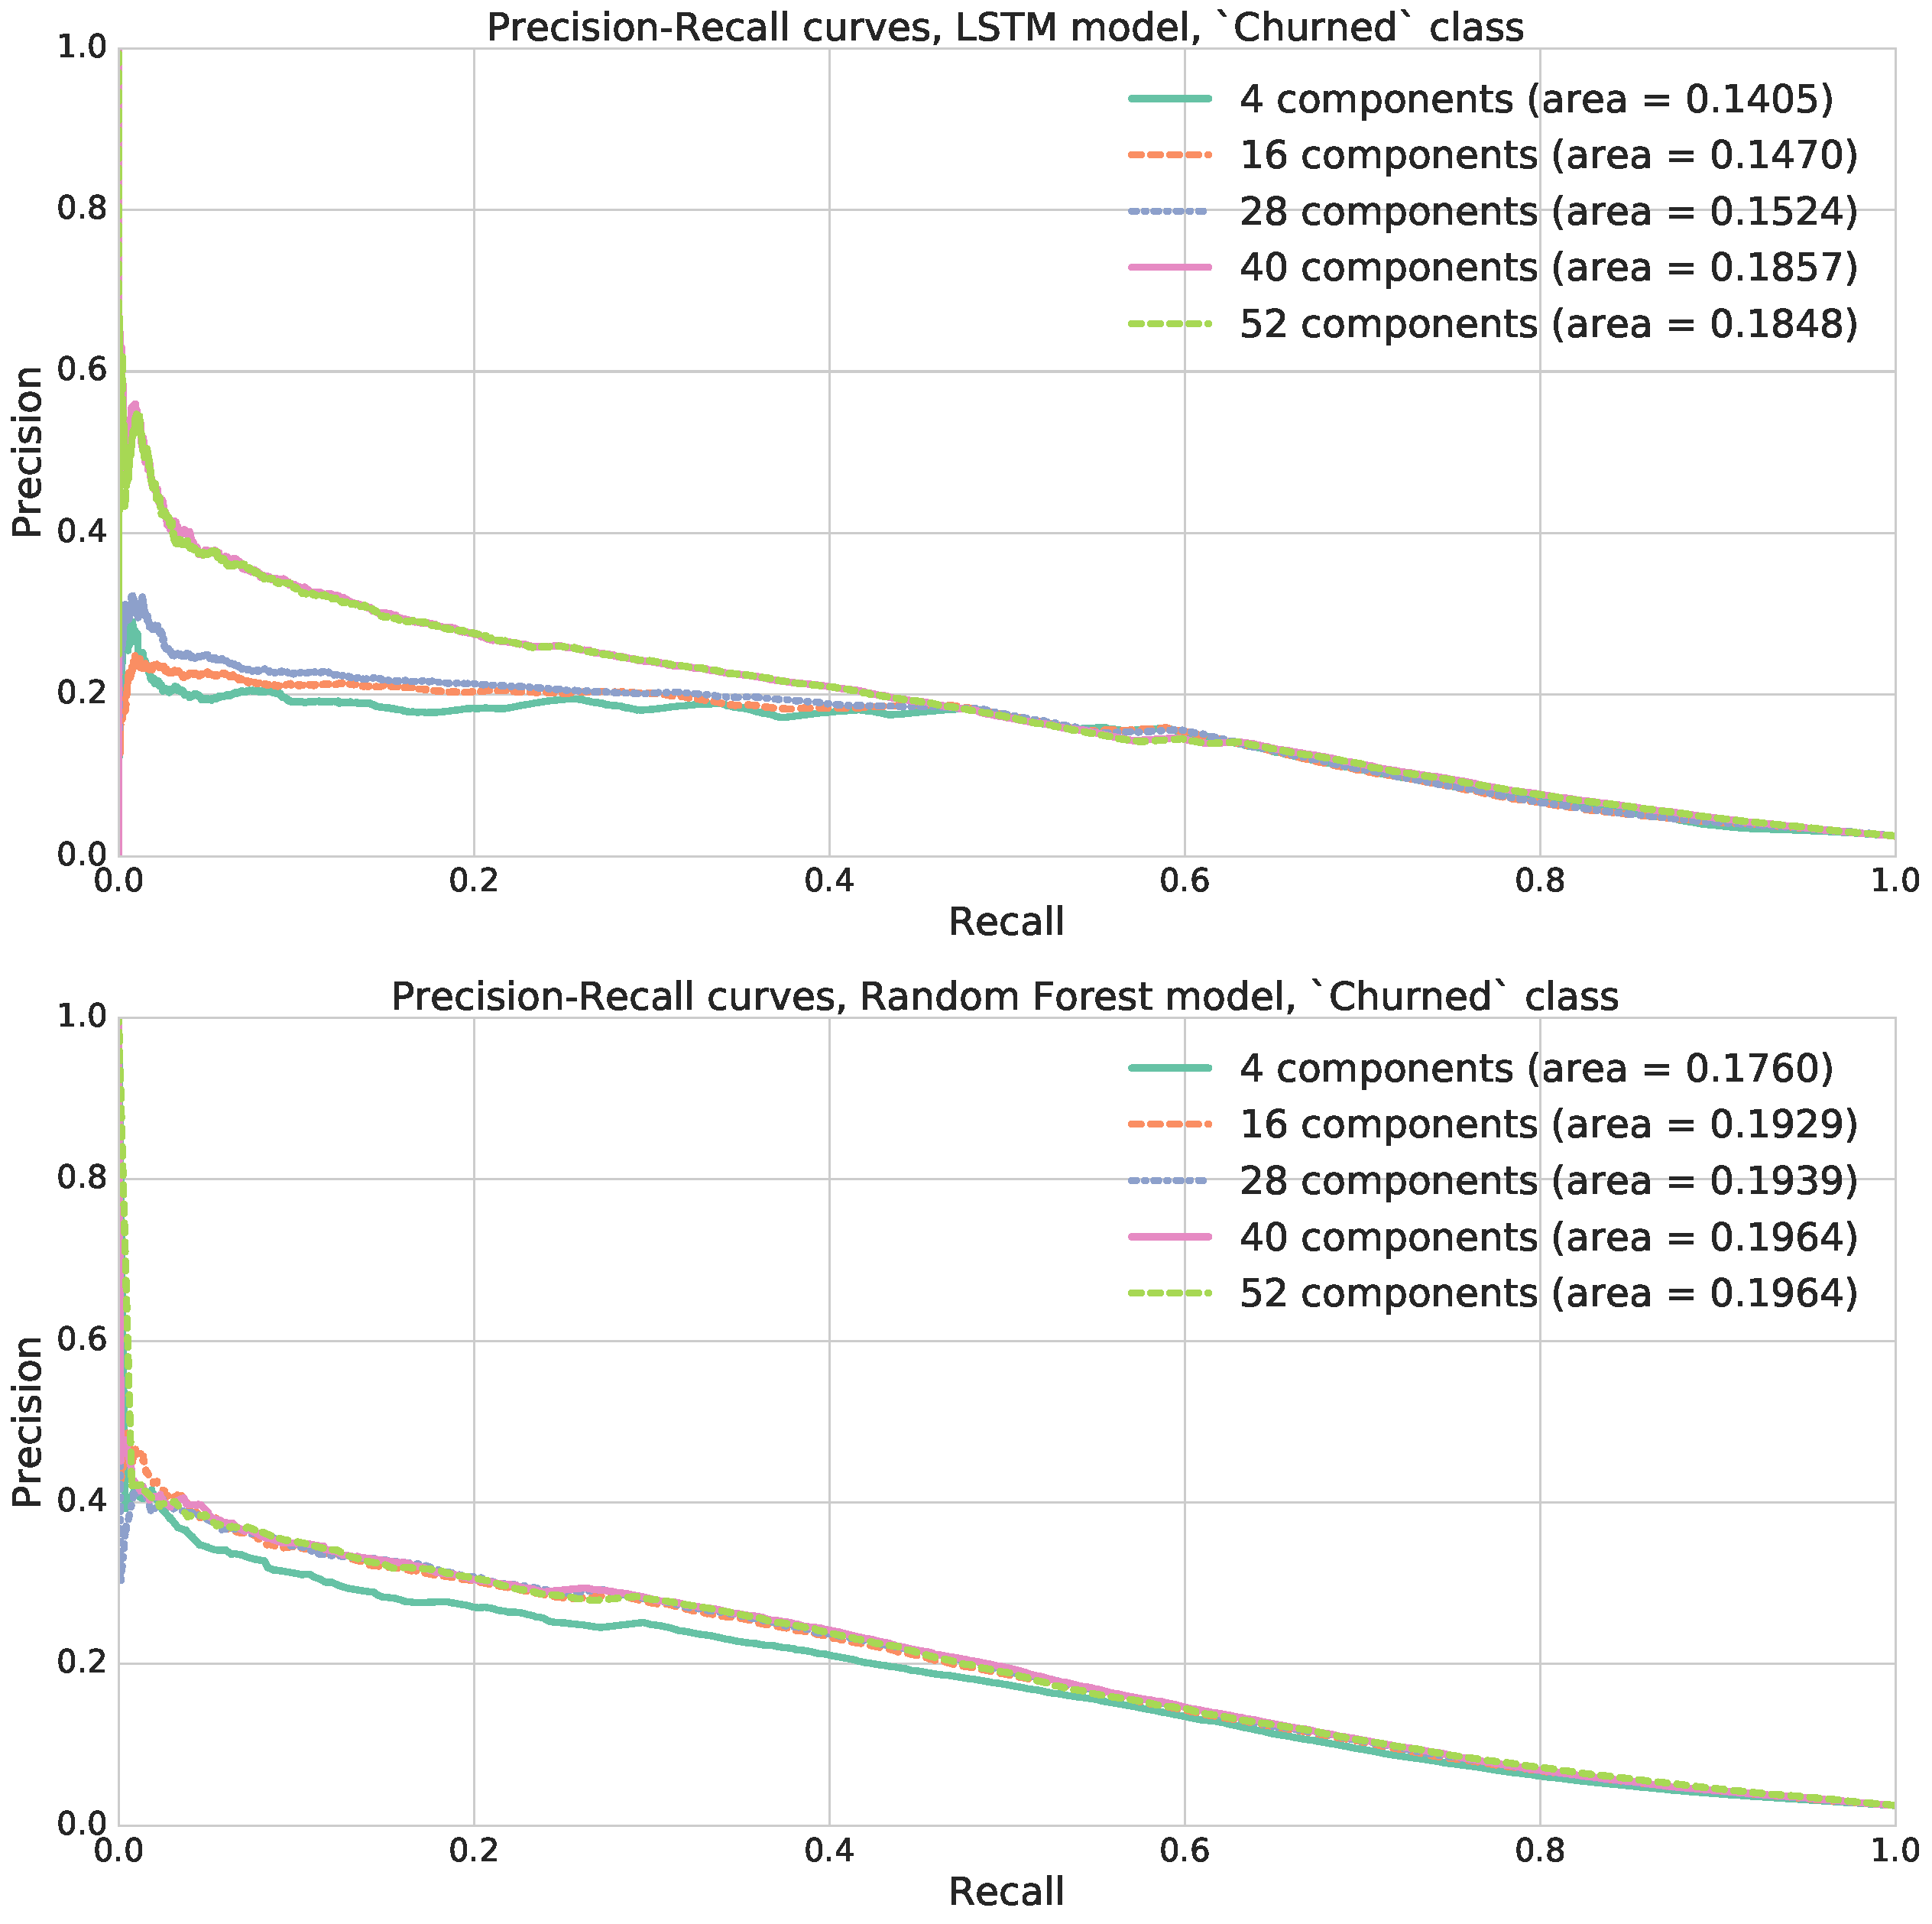
\includegraphics[width=1.0\textwidth,keepaspectratio]{figures/prc_dim_reduction.pdf}
    \caption{Precision-recall curves of the churned class for the dimensionality reduction experiment.}
    \label{fig:prc_dim_reduction}
\end{figure}

\begin{figure}
    \centering
    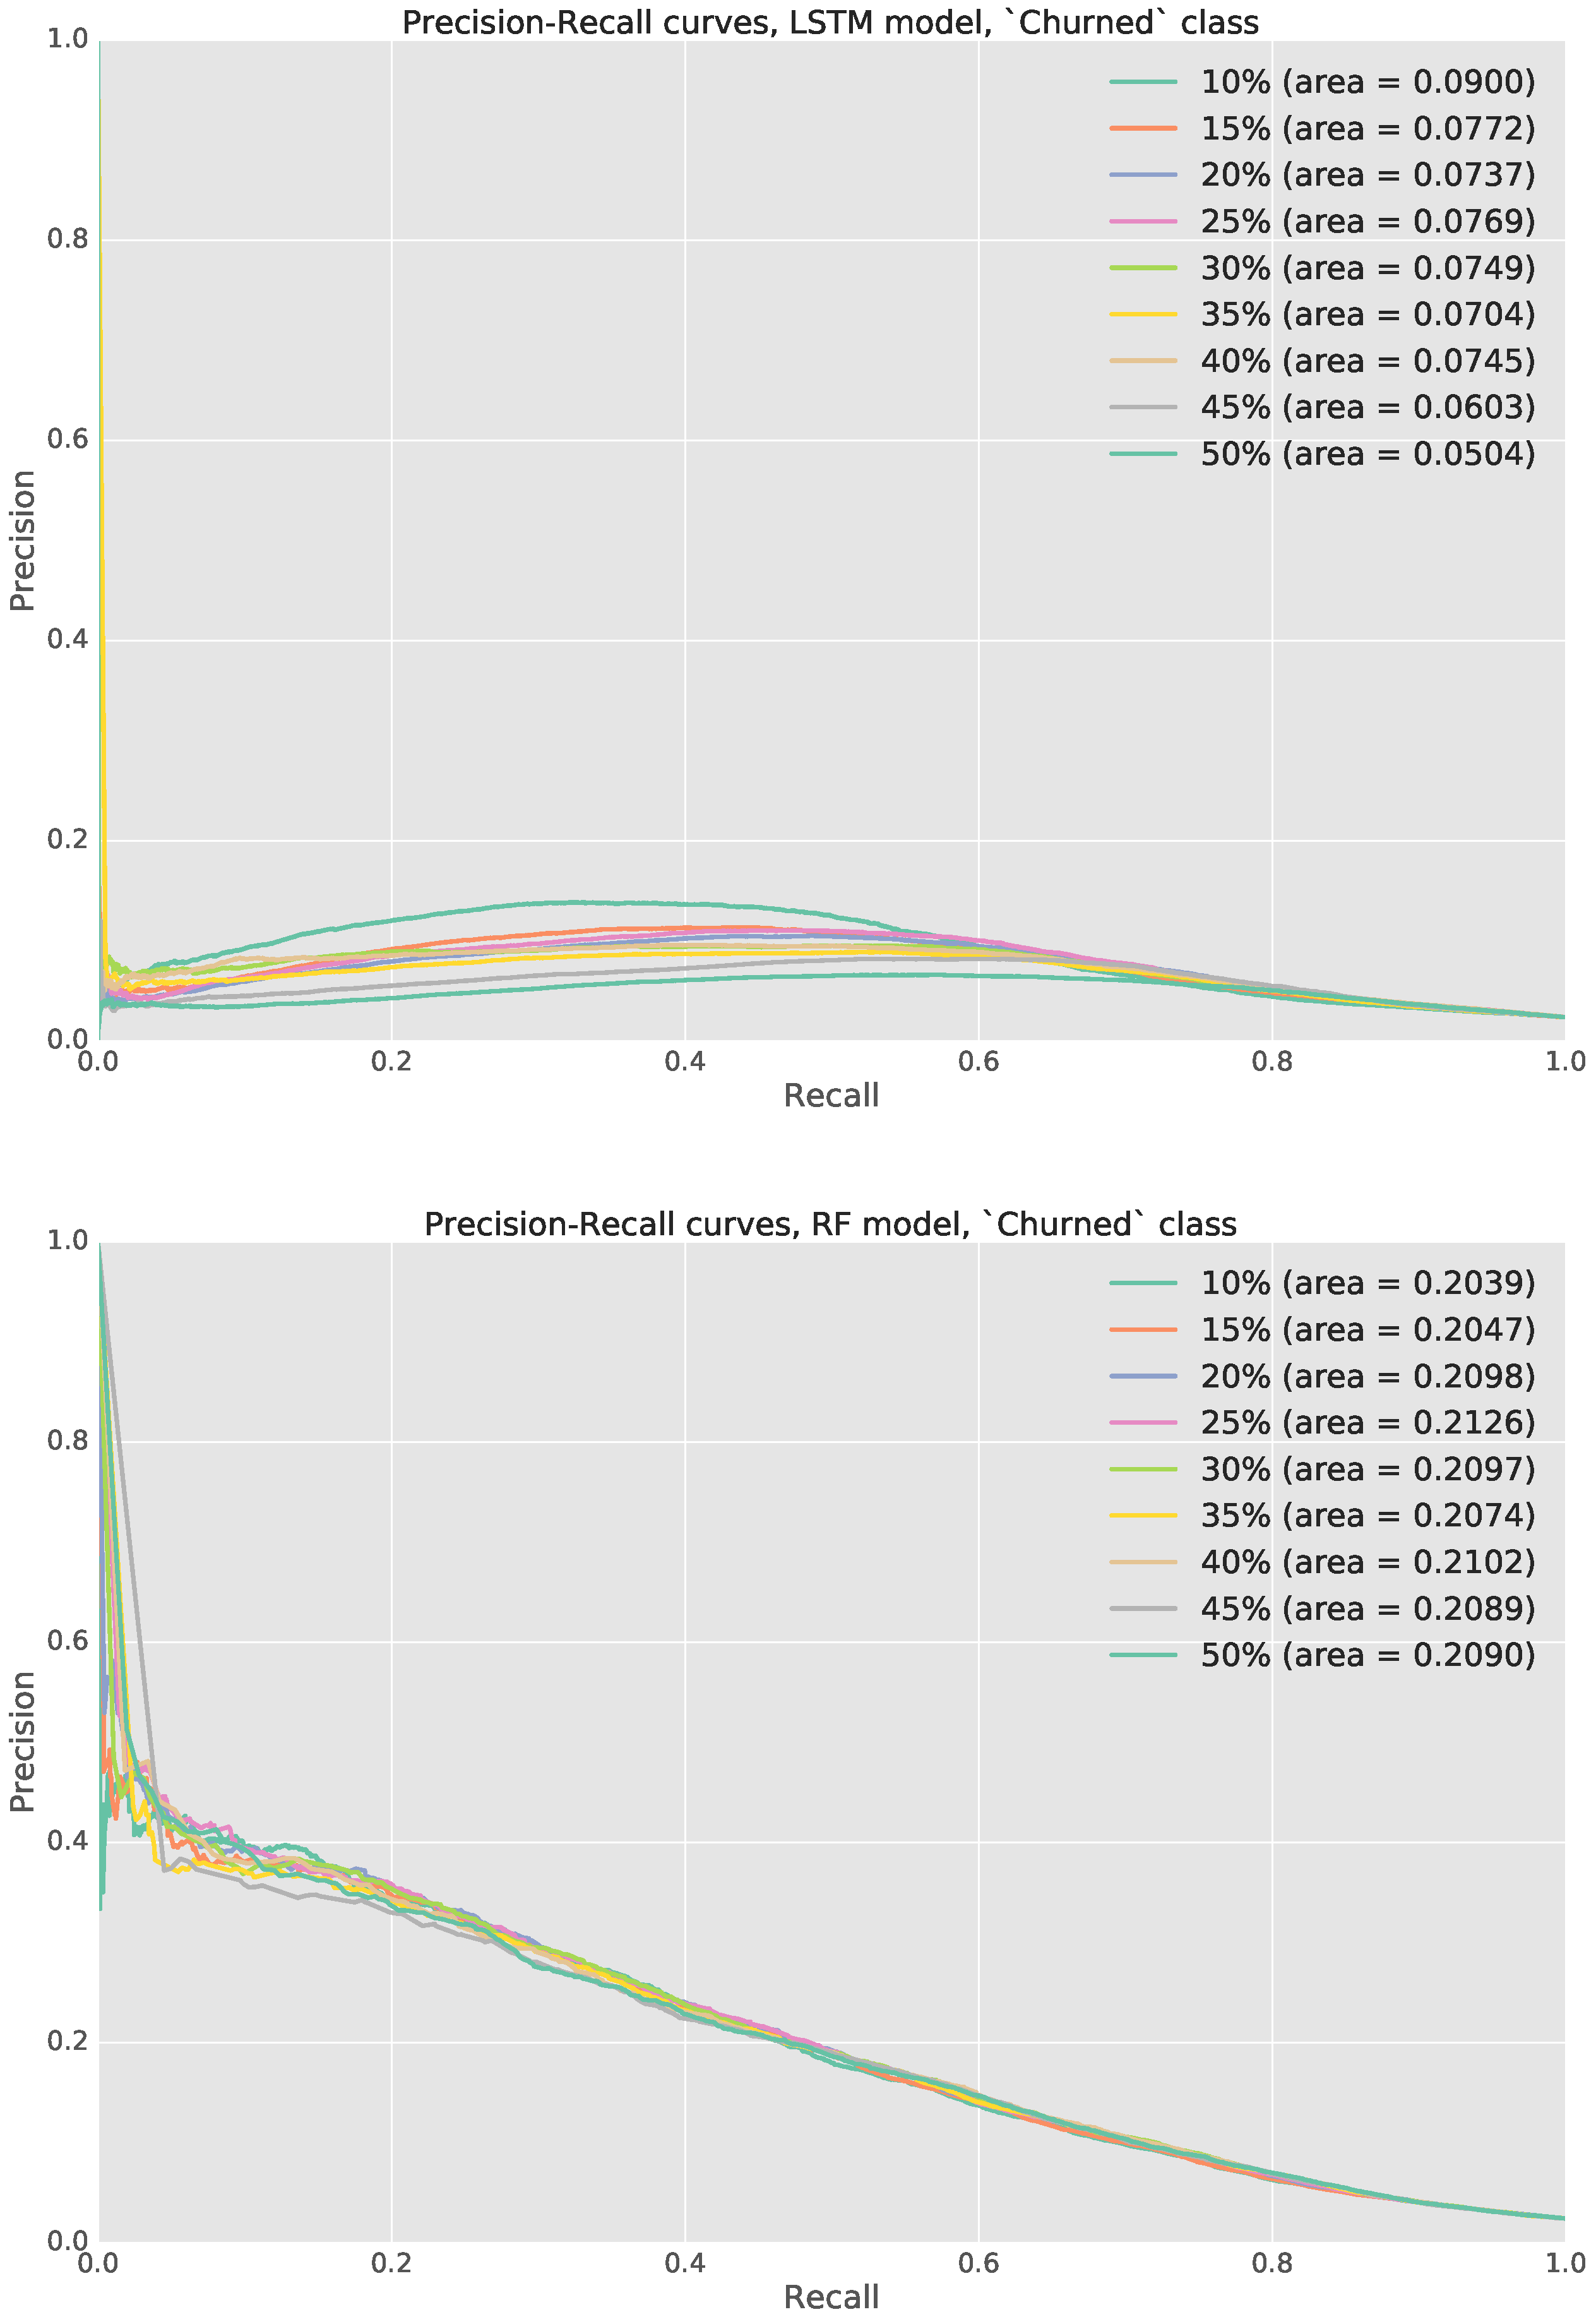
\includegraphics[width=1.0\textwidth,keepaspectratio]{figures/prc_class_balance.pdf}
    \caption{Precision-recall curves of the churned class for the class balance experiment.}
    \label{fig:prc_class_balance}
\end{figure}


\begin{figure}
    \centering
    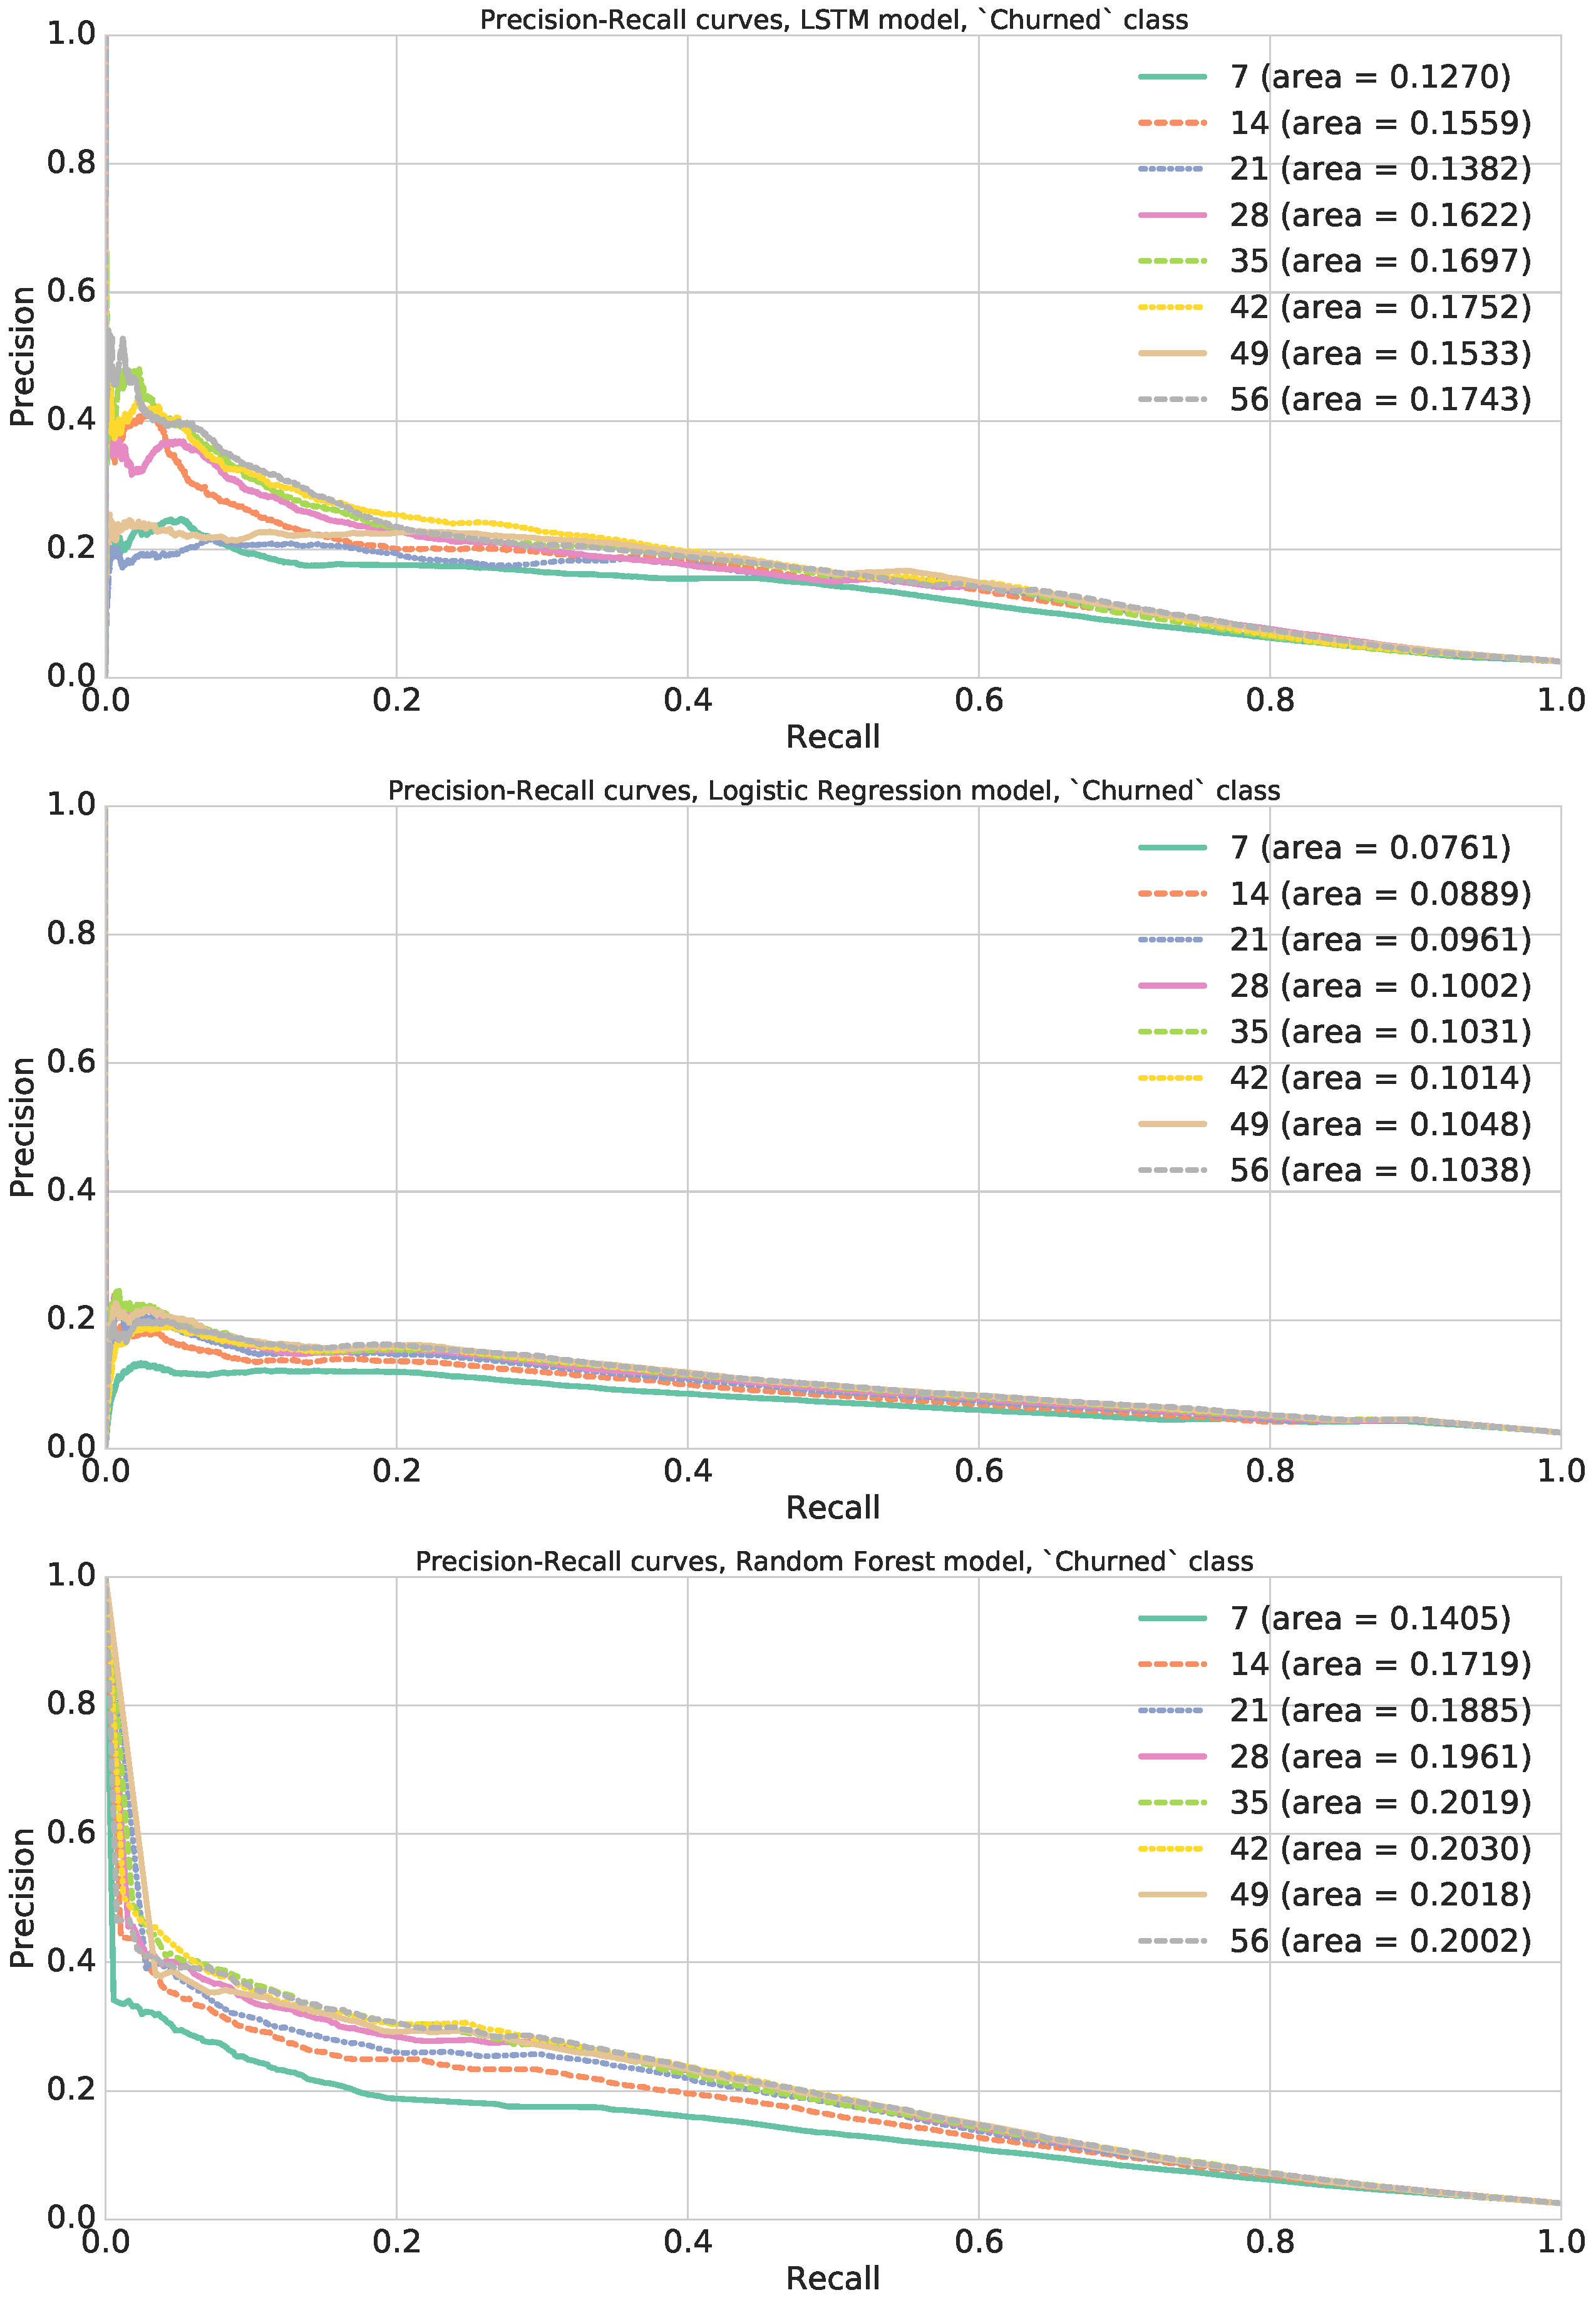
\includegraphics[width=1.0\textwidth,keepaspectratio]{figures/prc_obs_window.pdf}
    \caption{Precision-recall curves of the churned class for the observation window experiment.}
    \label{fig:prc_obs_window}
\end{figure}

\begin{figure}
    \centering
    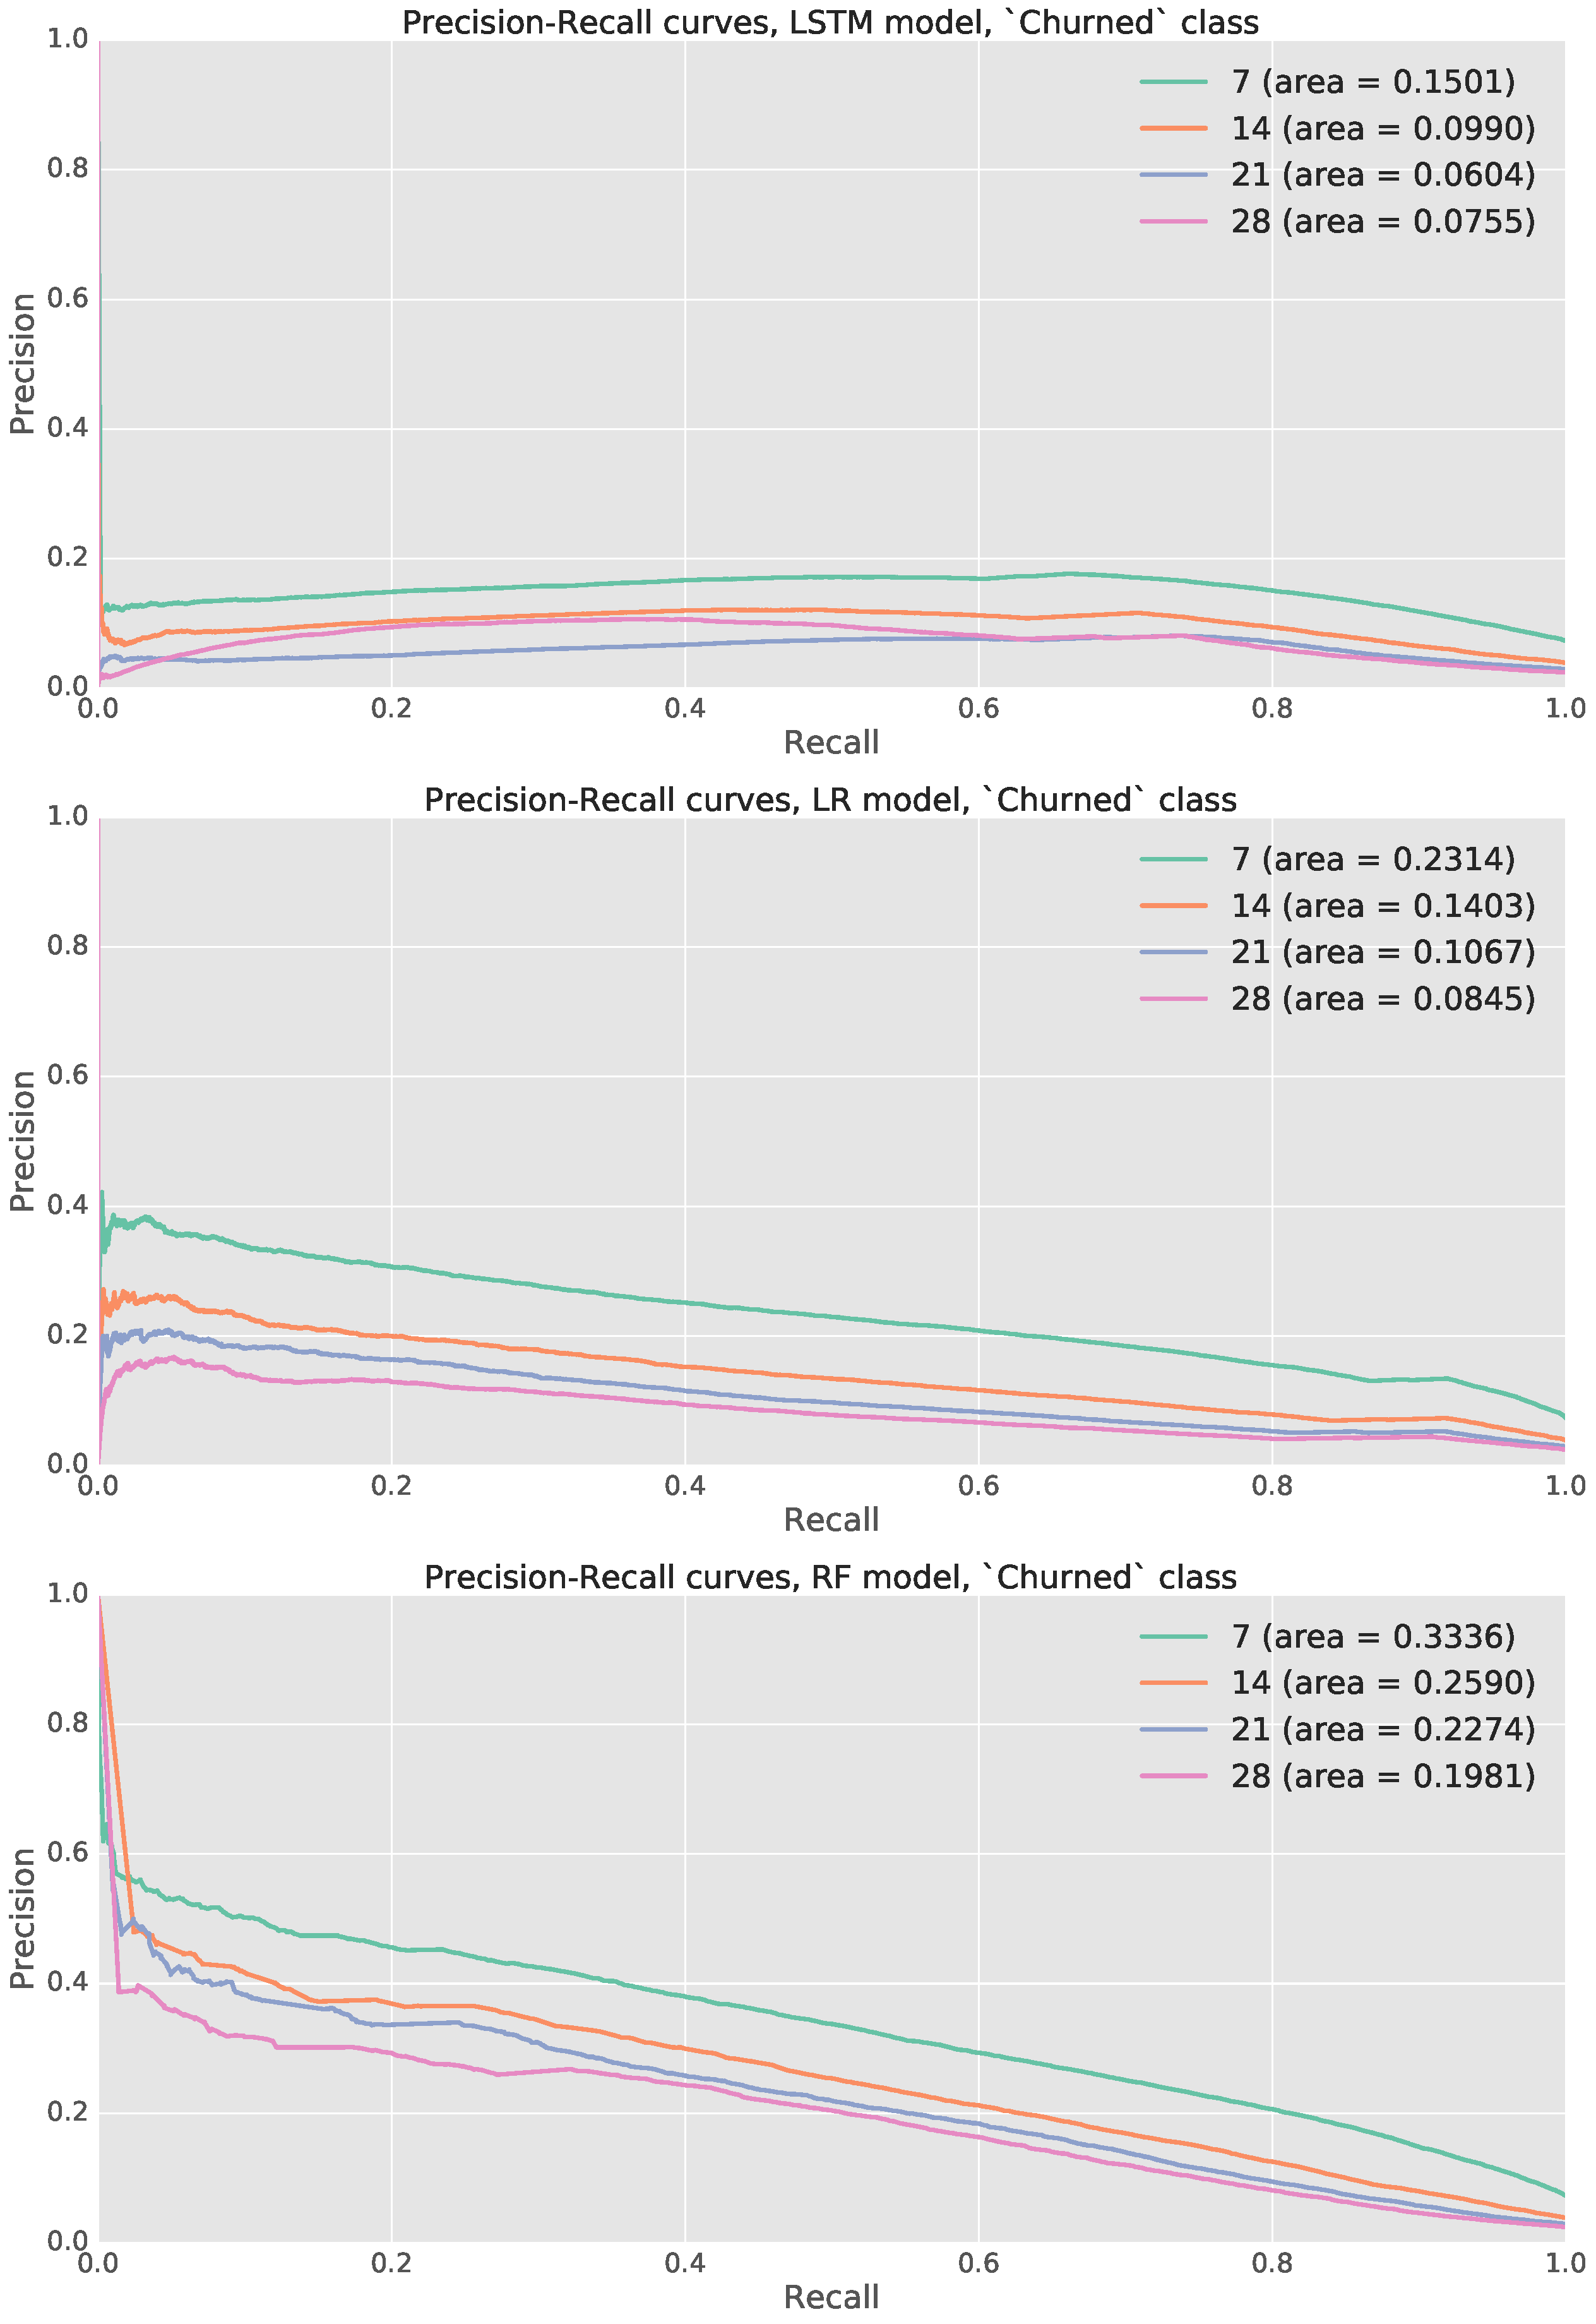
\includegraphics[width=1.0\textwidth,keepaspectratio]{figures/prc_pred_window.pdf}
    \caption{Precision-recall curves of the churned class for the prediction window experiment.}
    \label{fig:prc_pred_window}
\end{figure}

\clearpage

\section{ROC curves}

\begin{figure}[h]
    \centering
    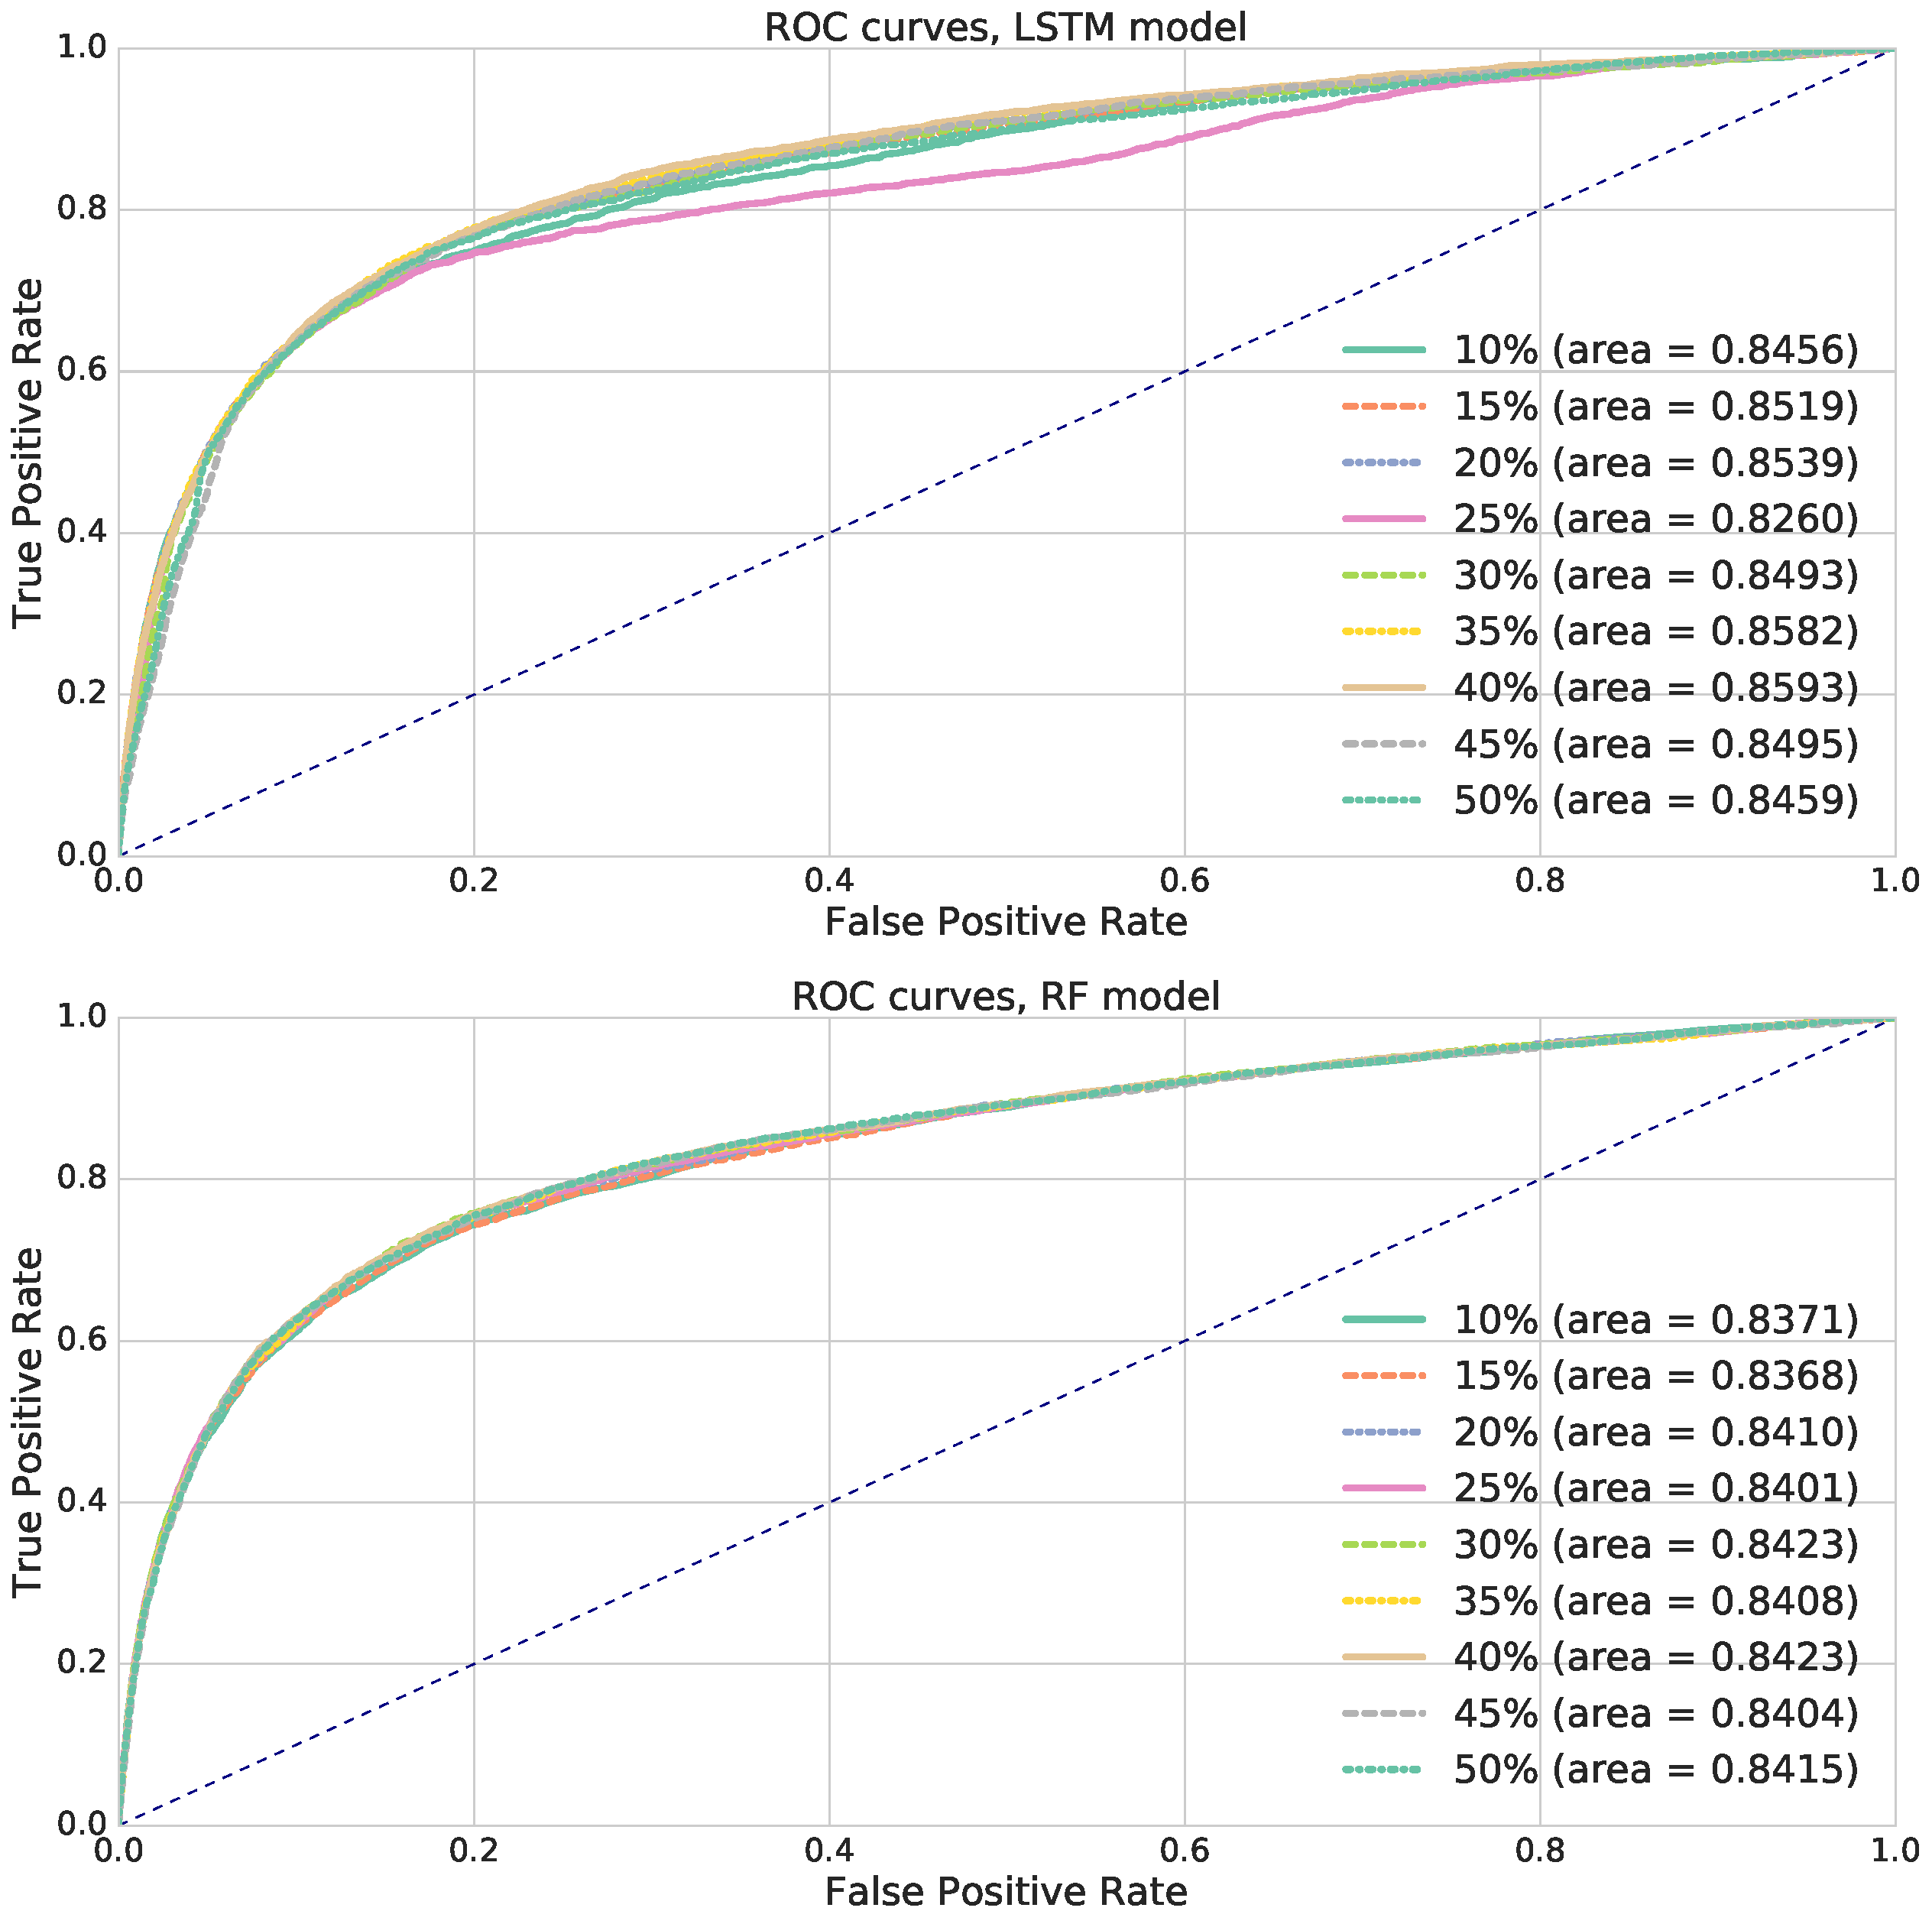
\includegraphics[width=1.0\textwidth,keepaspectratio]{figures/roc_class_balance.pdf}
    \caption{ROC curves for the class balance experiment}
    \label{fig:roc_class_balance}
\end{figure}

\begin{figure}
    \centering
    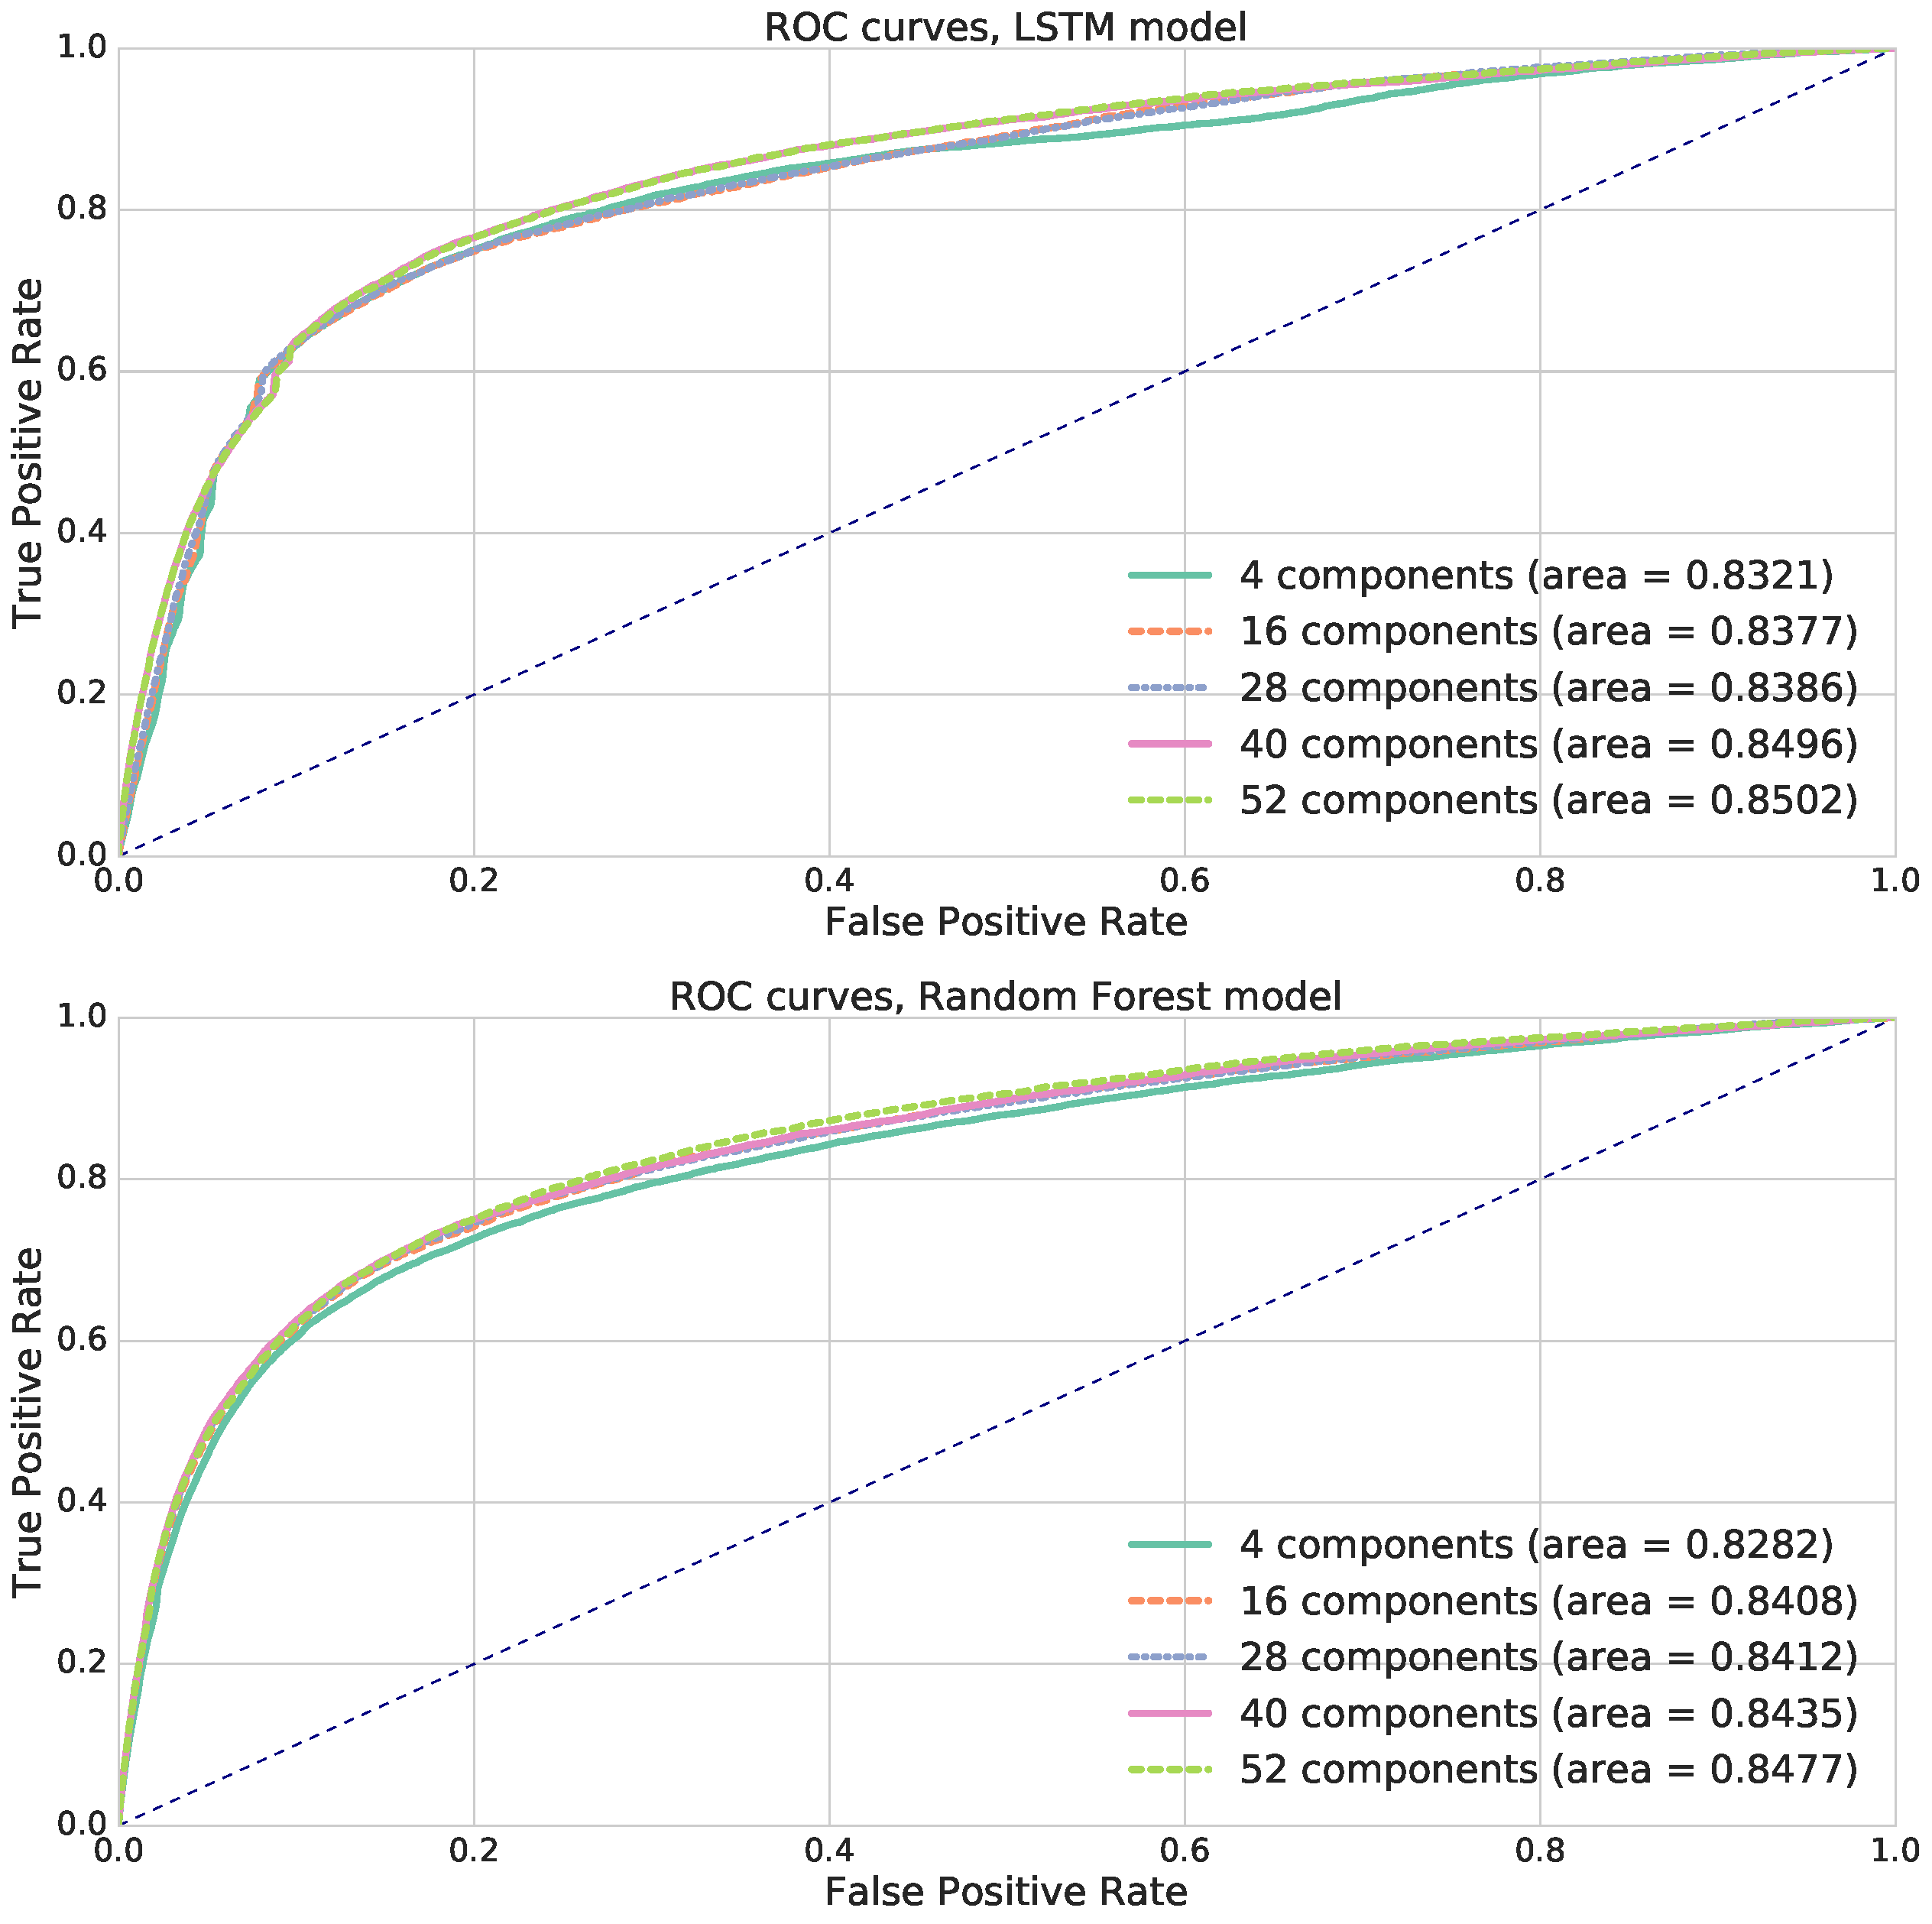
\includegraphics[width=1.0\textwidth,keepaspectratio]{figures/roc_dim_reduction.pdf}
    \caption{ROC curves for the dimensionality reduction experiment}
    \label{fig:roc_dim_reduction}
\end{figure}

\begin{figure}
    \centering
    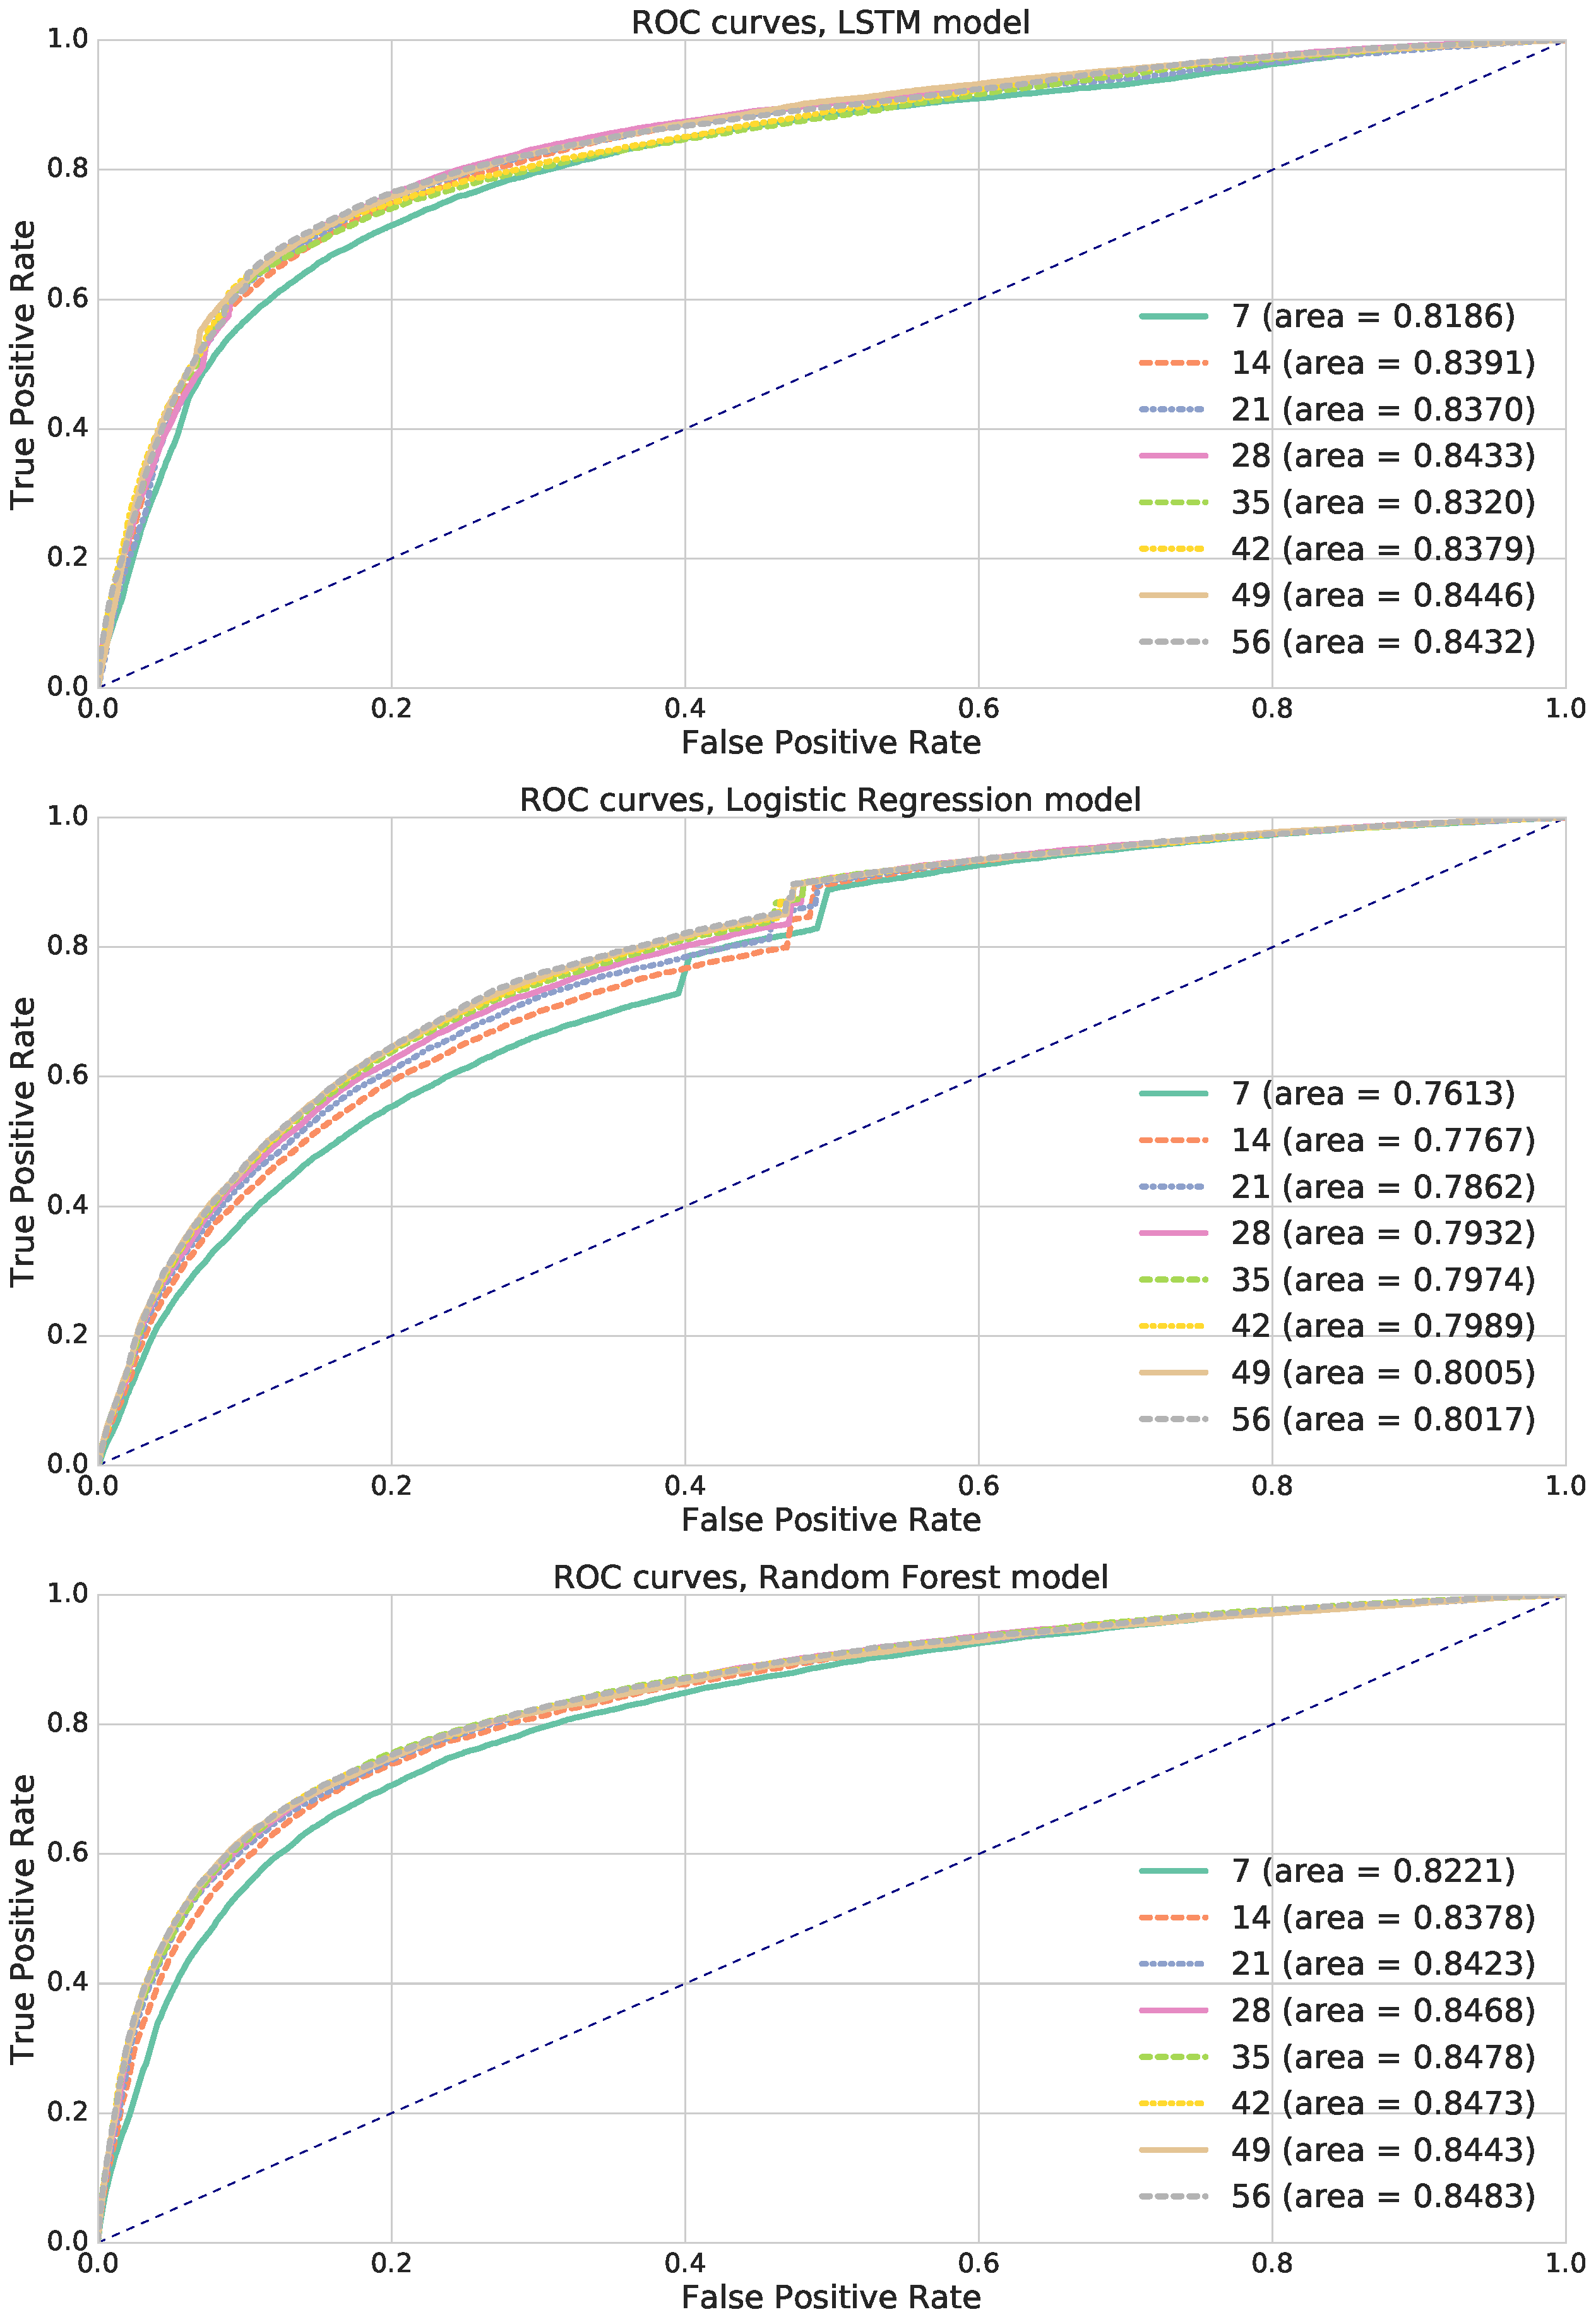
\includegraphics[width=1.0\textwidth,keepaspectratio]{figures/roc_obs_window.pdf}
    \caption{ROC curves for the observation window experiment}
    \label{fig:roc_obs_window}
\end{figure}

\begin{figure}
    \centering
    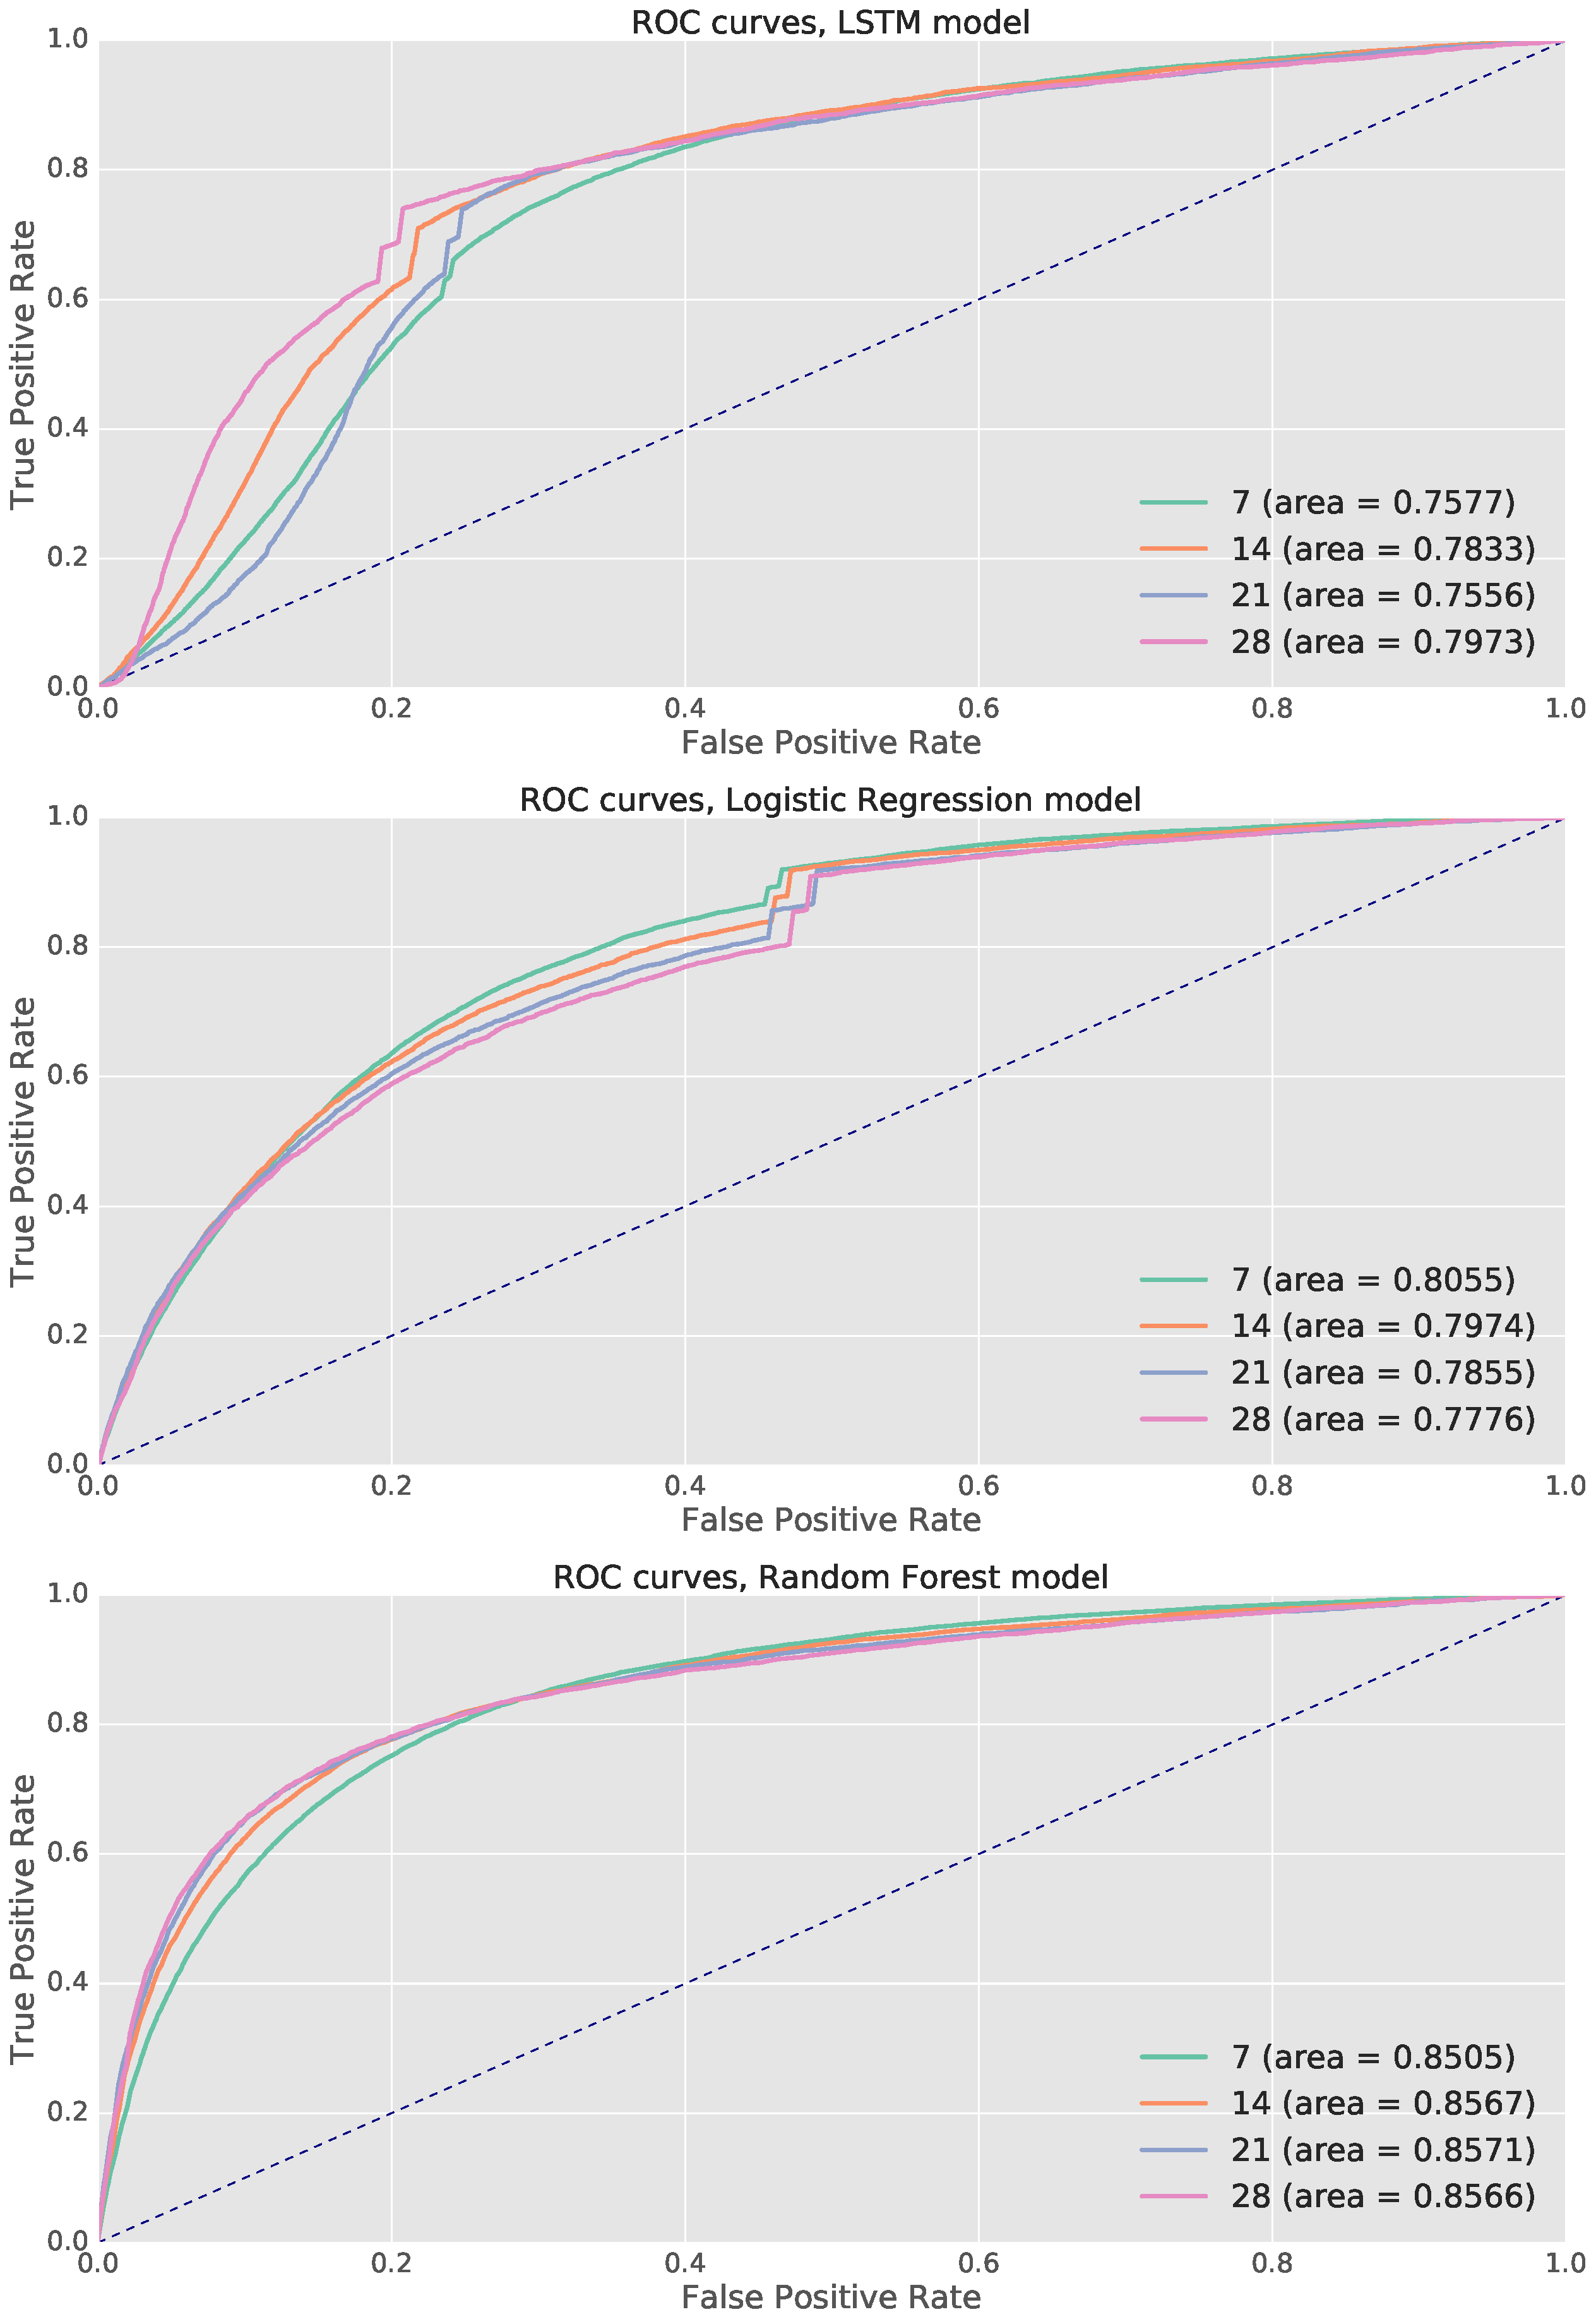
\includegraphics[width=1.0\textwidth,keepaspectratio]{figures/roc_pred_window.pdf}
    \caption{ROC curves for the prediction window experiment}
    \label{fig:roc_pred_window}
\end{figure}


% --------------------

\end{document}
